


\section{Ingreso Familiar}

            \begin{itemize}
                    \item Pero hay una brecha de género enorme, especialmente en los percentiles más bajos de ingreso.
                    \item El rezago en el ingreso de las mujeres con respecto al de los hombres es de más de 10 años.
                \end{itemize}
    
    \subsection{Ingreso Laboral}
 %%%% Include figures
    \begin{figure}[H]
    \caption[Percentil 25 del ingreso laboral por ciudades principales - 2019]{\label{map_result_2}}
        \begin{center}
        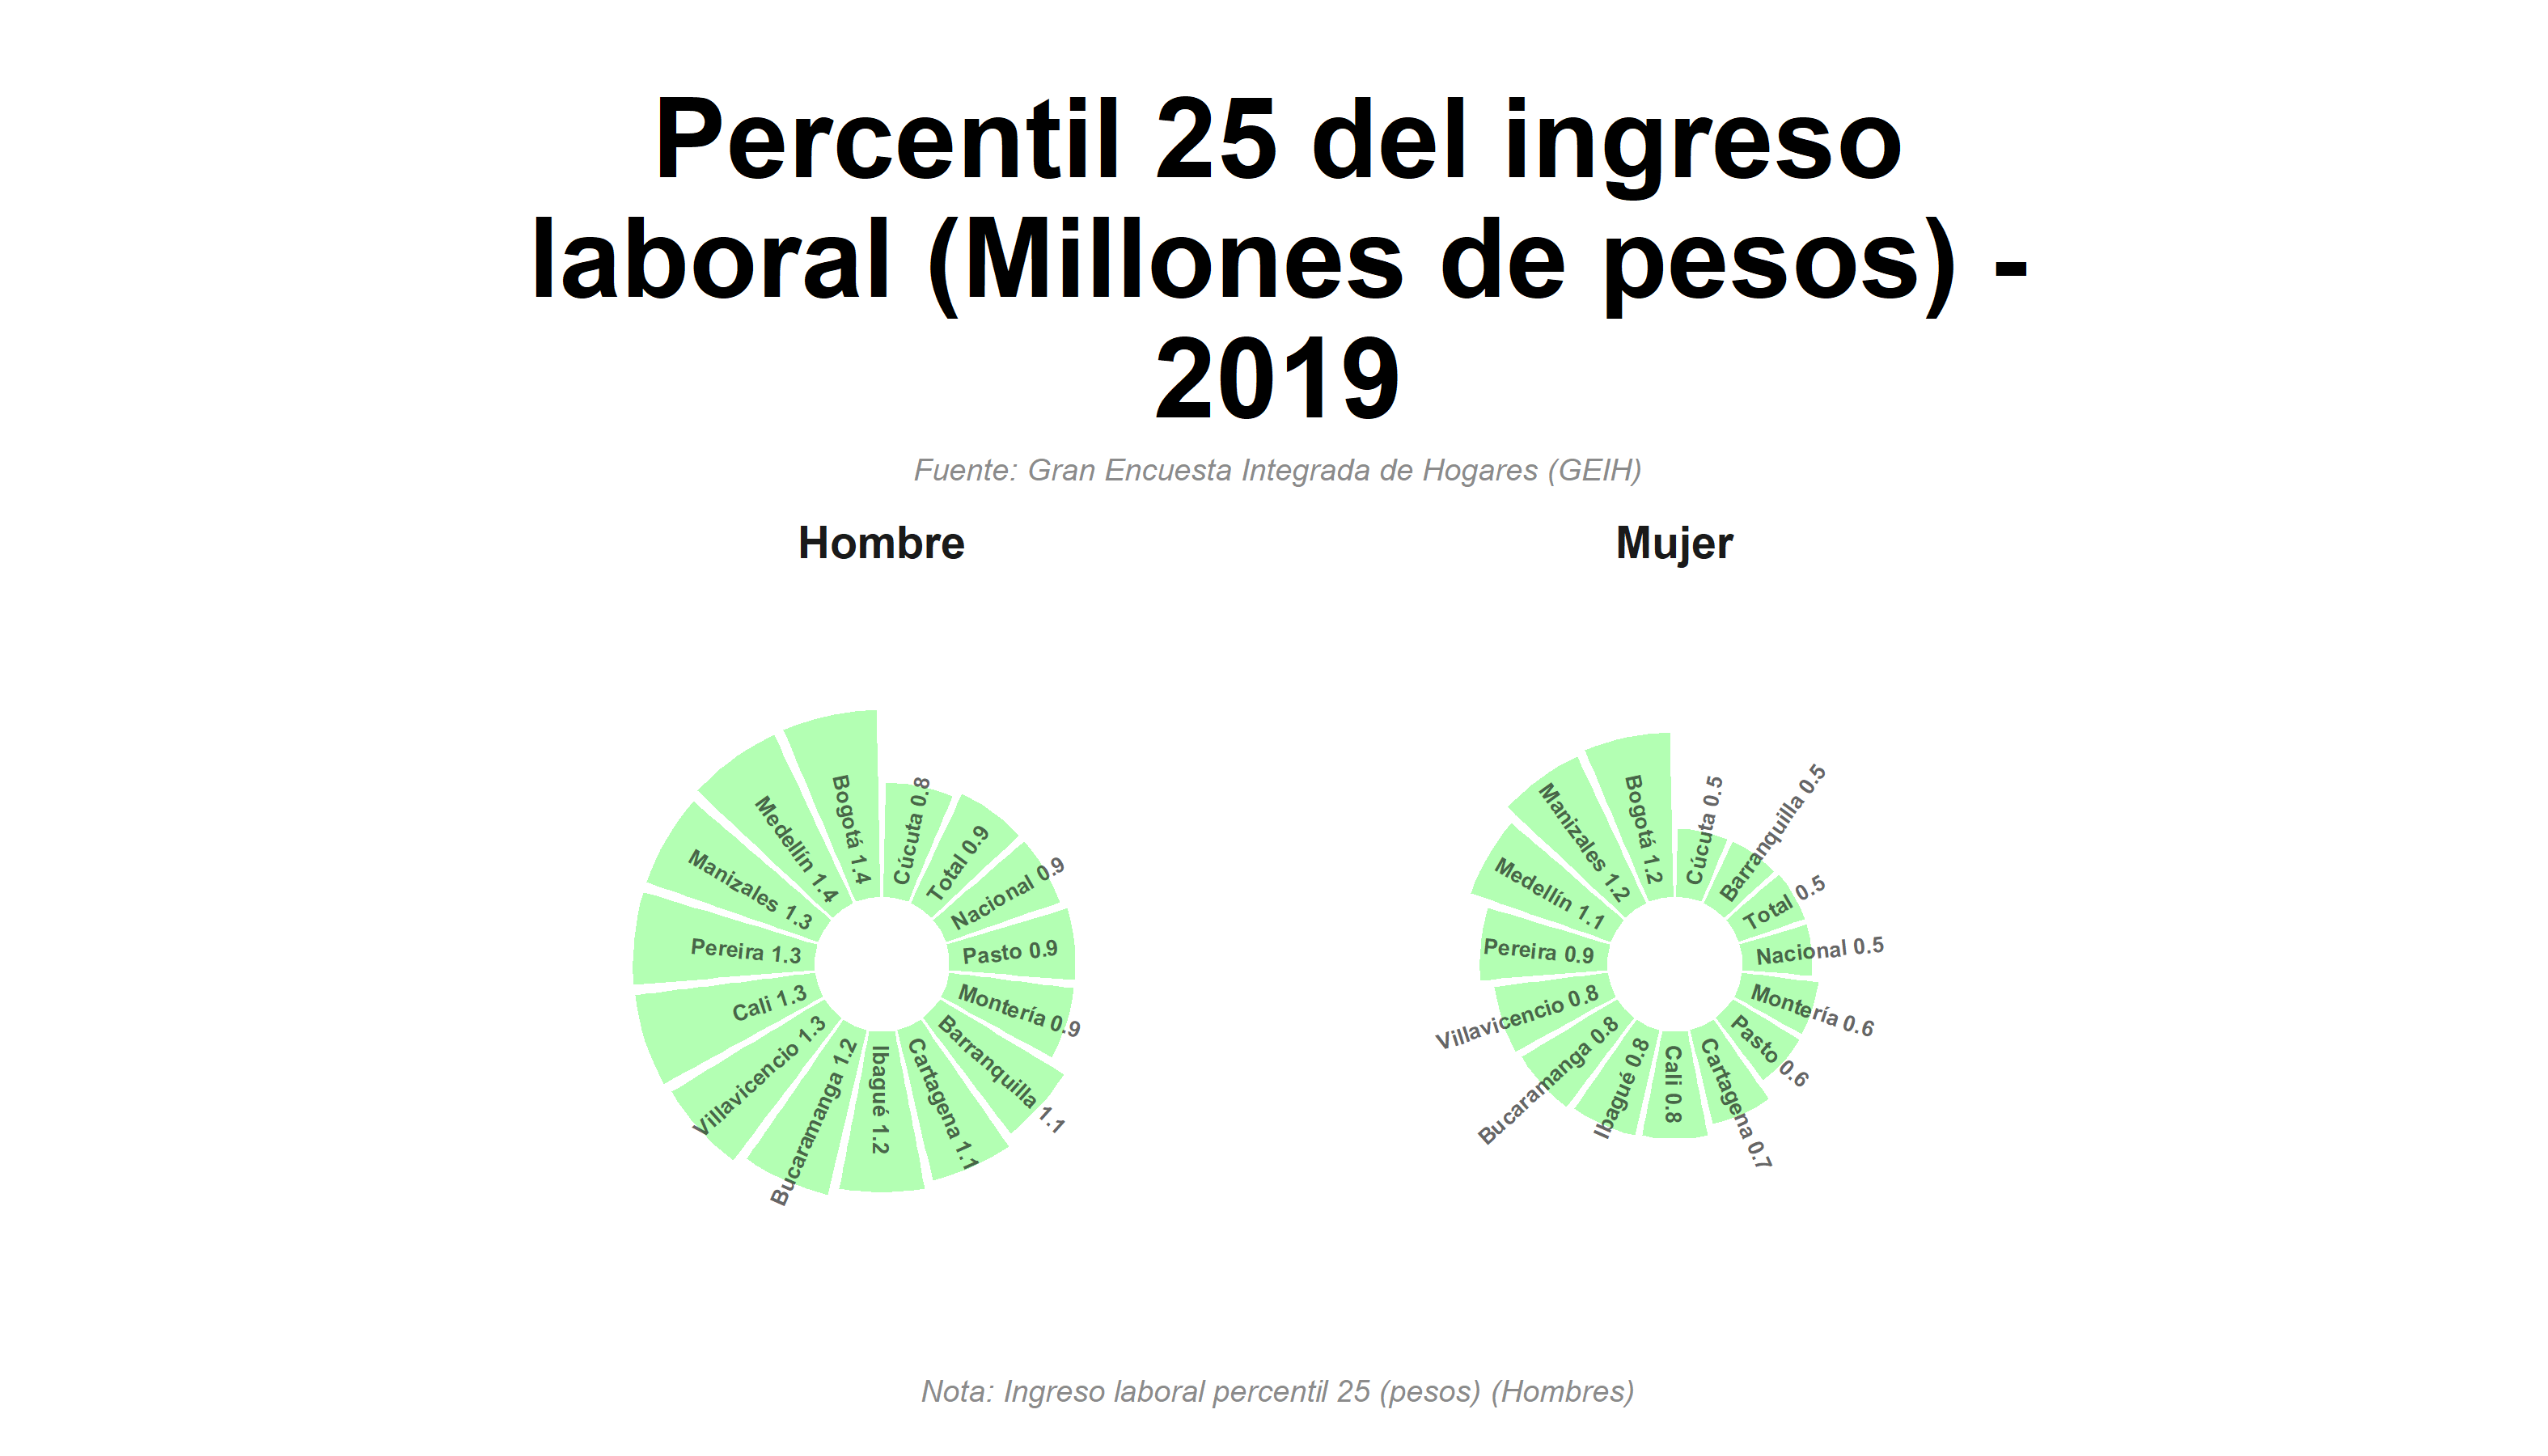
\includegraphics[width=\textwidth,keepaspectratio]{img/var_2_static.png}
        \end{center}
    \end{figure}
            \begin{itemize}
                    \item Hay una diferencia de ingreso de más de un millón entre la ciudad de menor ingreso y la de mayor (Cúcuta -  Bogotá).
                    \item Todas las ciudades principales están por encima del promedio nacional a excepción de Cúcuta.
                \end{itemize}

 %%%% Include figures
    \begin{figure}[H]
        \caption{Percentil 25 del ingreso laboral por ciudades principales para minorías - 2020 \label{map_result_2} }
        \begin{center}
        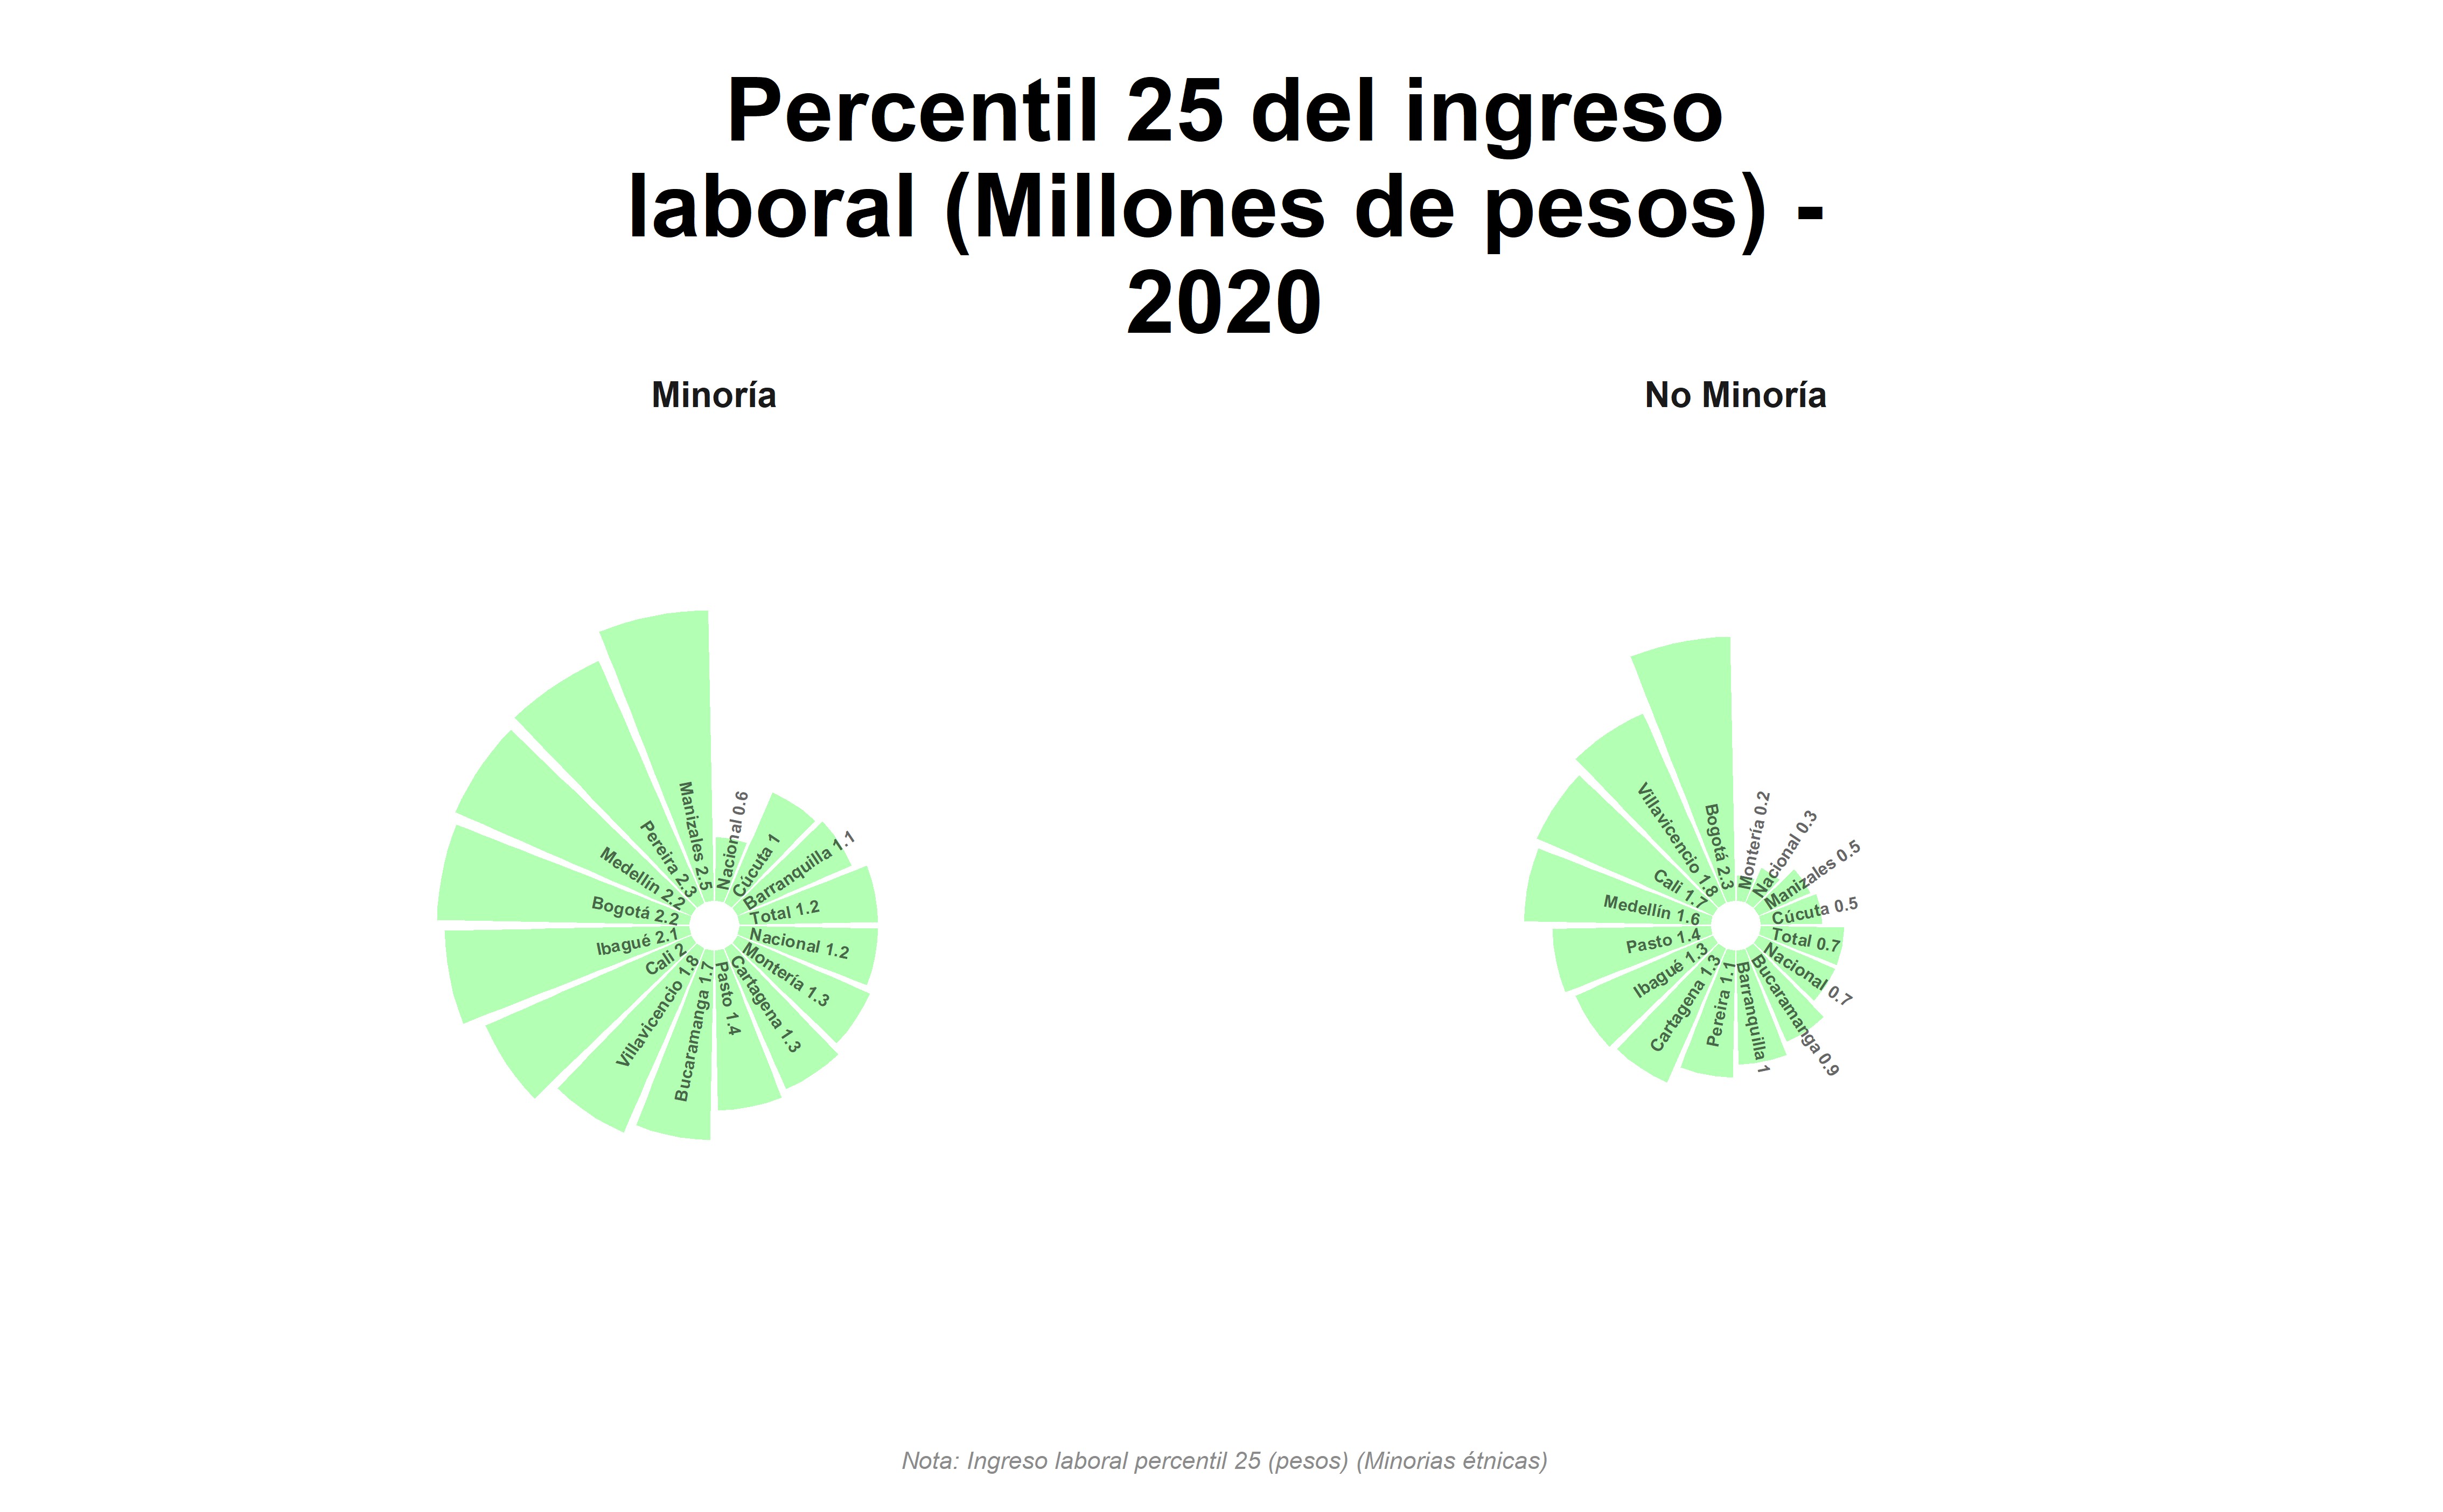
\includegraphics[width=\textwidth,keepaspectratio]{img/var_1_static.png}
        \end{center}
    \end{figure}
            \begin{itemize}
                    \item Hay una diferencia de ingreso de alrededor de 2 millones entre la ciudad de mayor ingreso y la de menor para minorías (Cúcuta -  Manizales) y no minorías (Montería - Bogotá).
                    \item Todas las ciudades principales están por encima del promedio nacional a excepción de Montería en el caso de las no minorías.
                    \item En general las minorías tienen ingresos mayores con respecto a las no minorías en el percentil más bajo de ingresos.
                \end{itemize}

%%%% Include figures
    \begin{figure}[H]
        \caption{Percentil 25 del ingreso laboral por ciudades principales - 2010 VS 2019 \label{map_result_2} }
        \begin{center}
        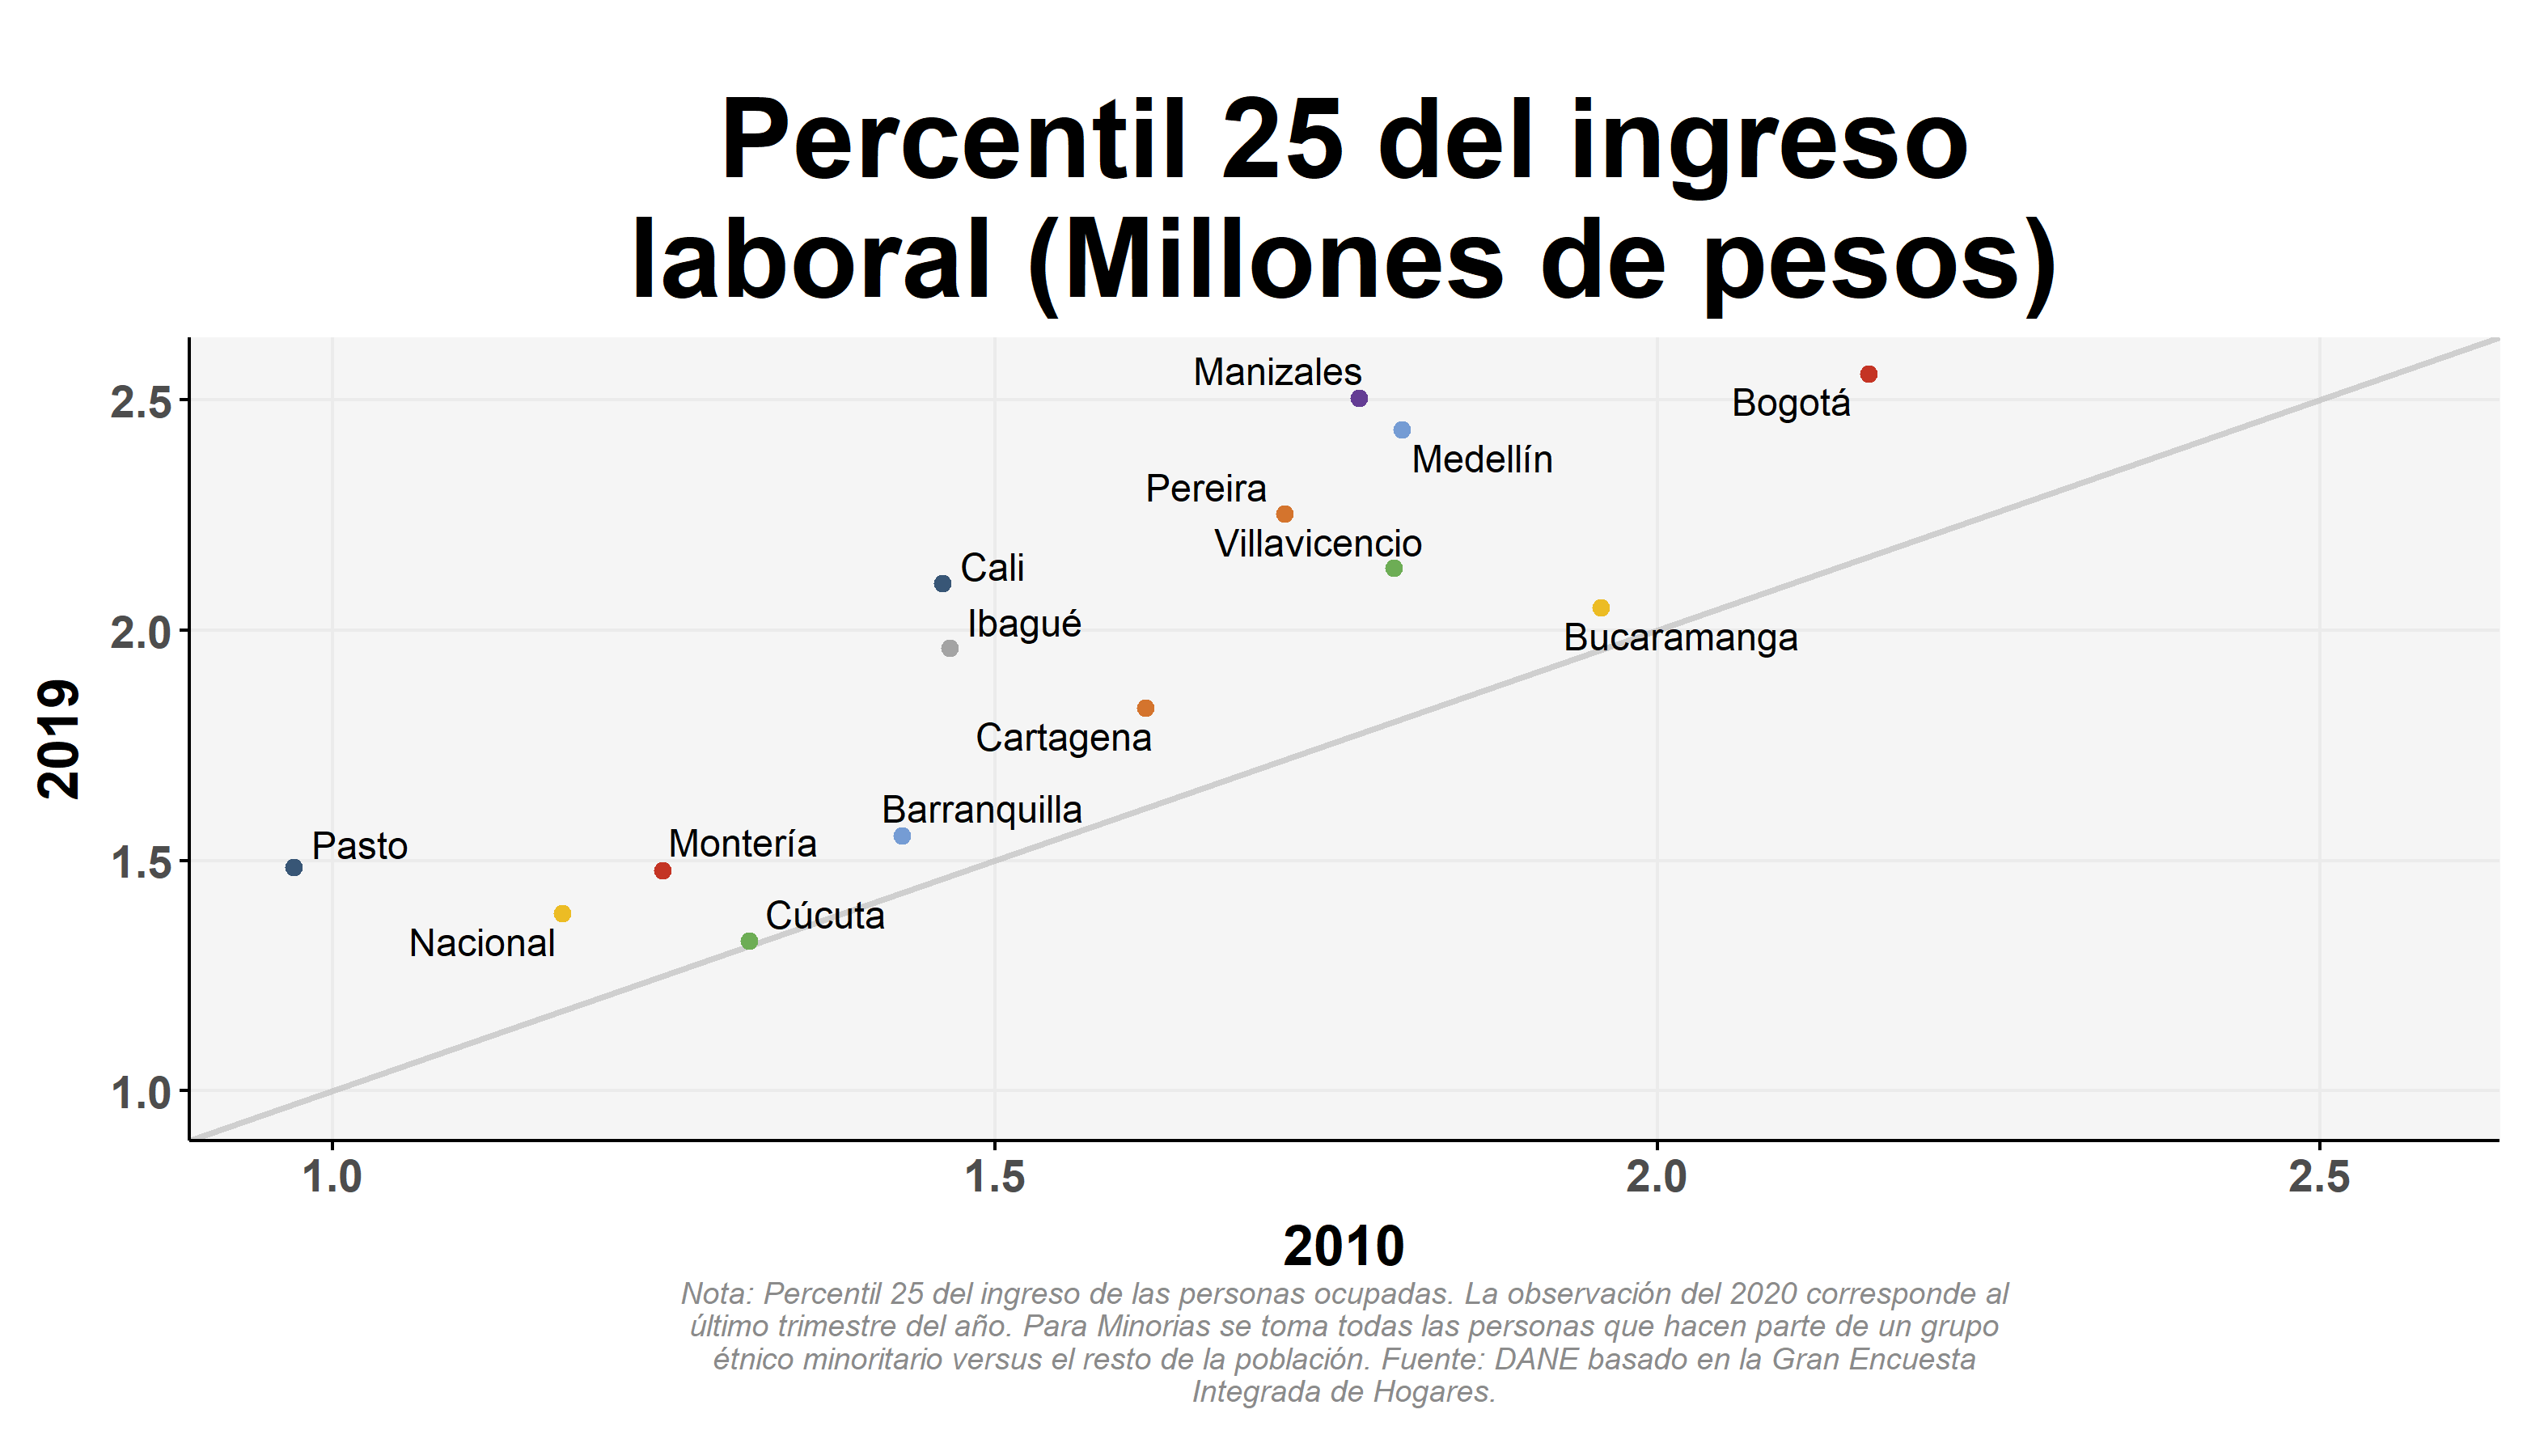
\includegraphics[width=\textwidth,keepaspectratio]{img/var_2_scatter_time.png}
        \end{center}
    \end{figure}
            \begin{itemize}
                    \item Todas las ciudades mejoraron en los últimos 10 años el ingreso laboral en el percentil a excepción de Cúcuta que se mantiene igual.
                    \item Ciudades que hace 10 años tenían similares ingresos pero unas mejoraron más significativamente que otras, caso Ibagué y Cali, y Villavicencio y Medellín.
                \end{itemize}

%%%% Include figures
    \begin{figure}[H]
        \caption{Percentil 25 del ingreso laboral por género \label{map_result_2} }
        \begin{center}
        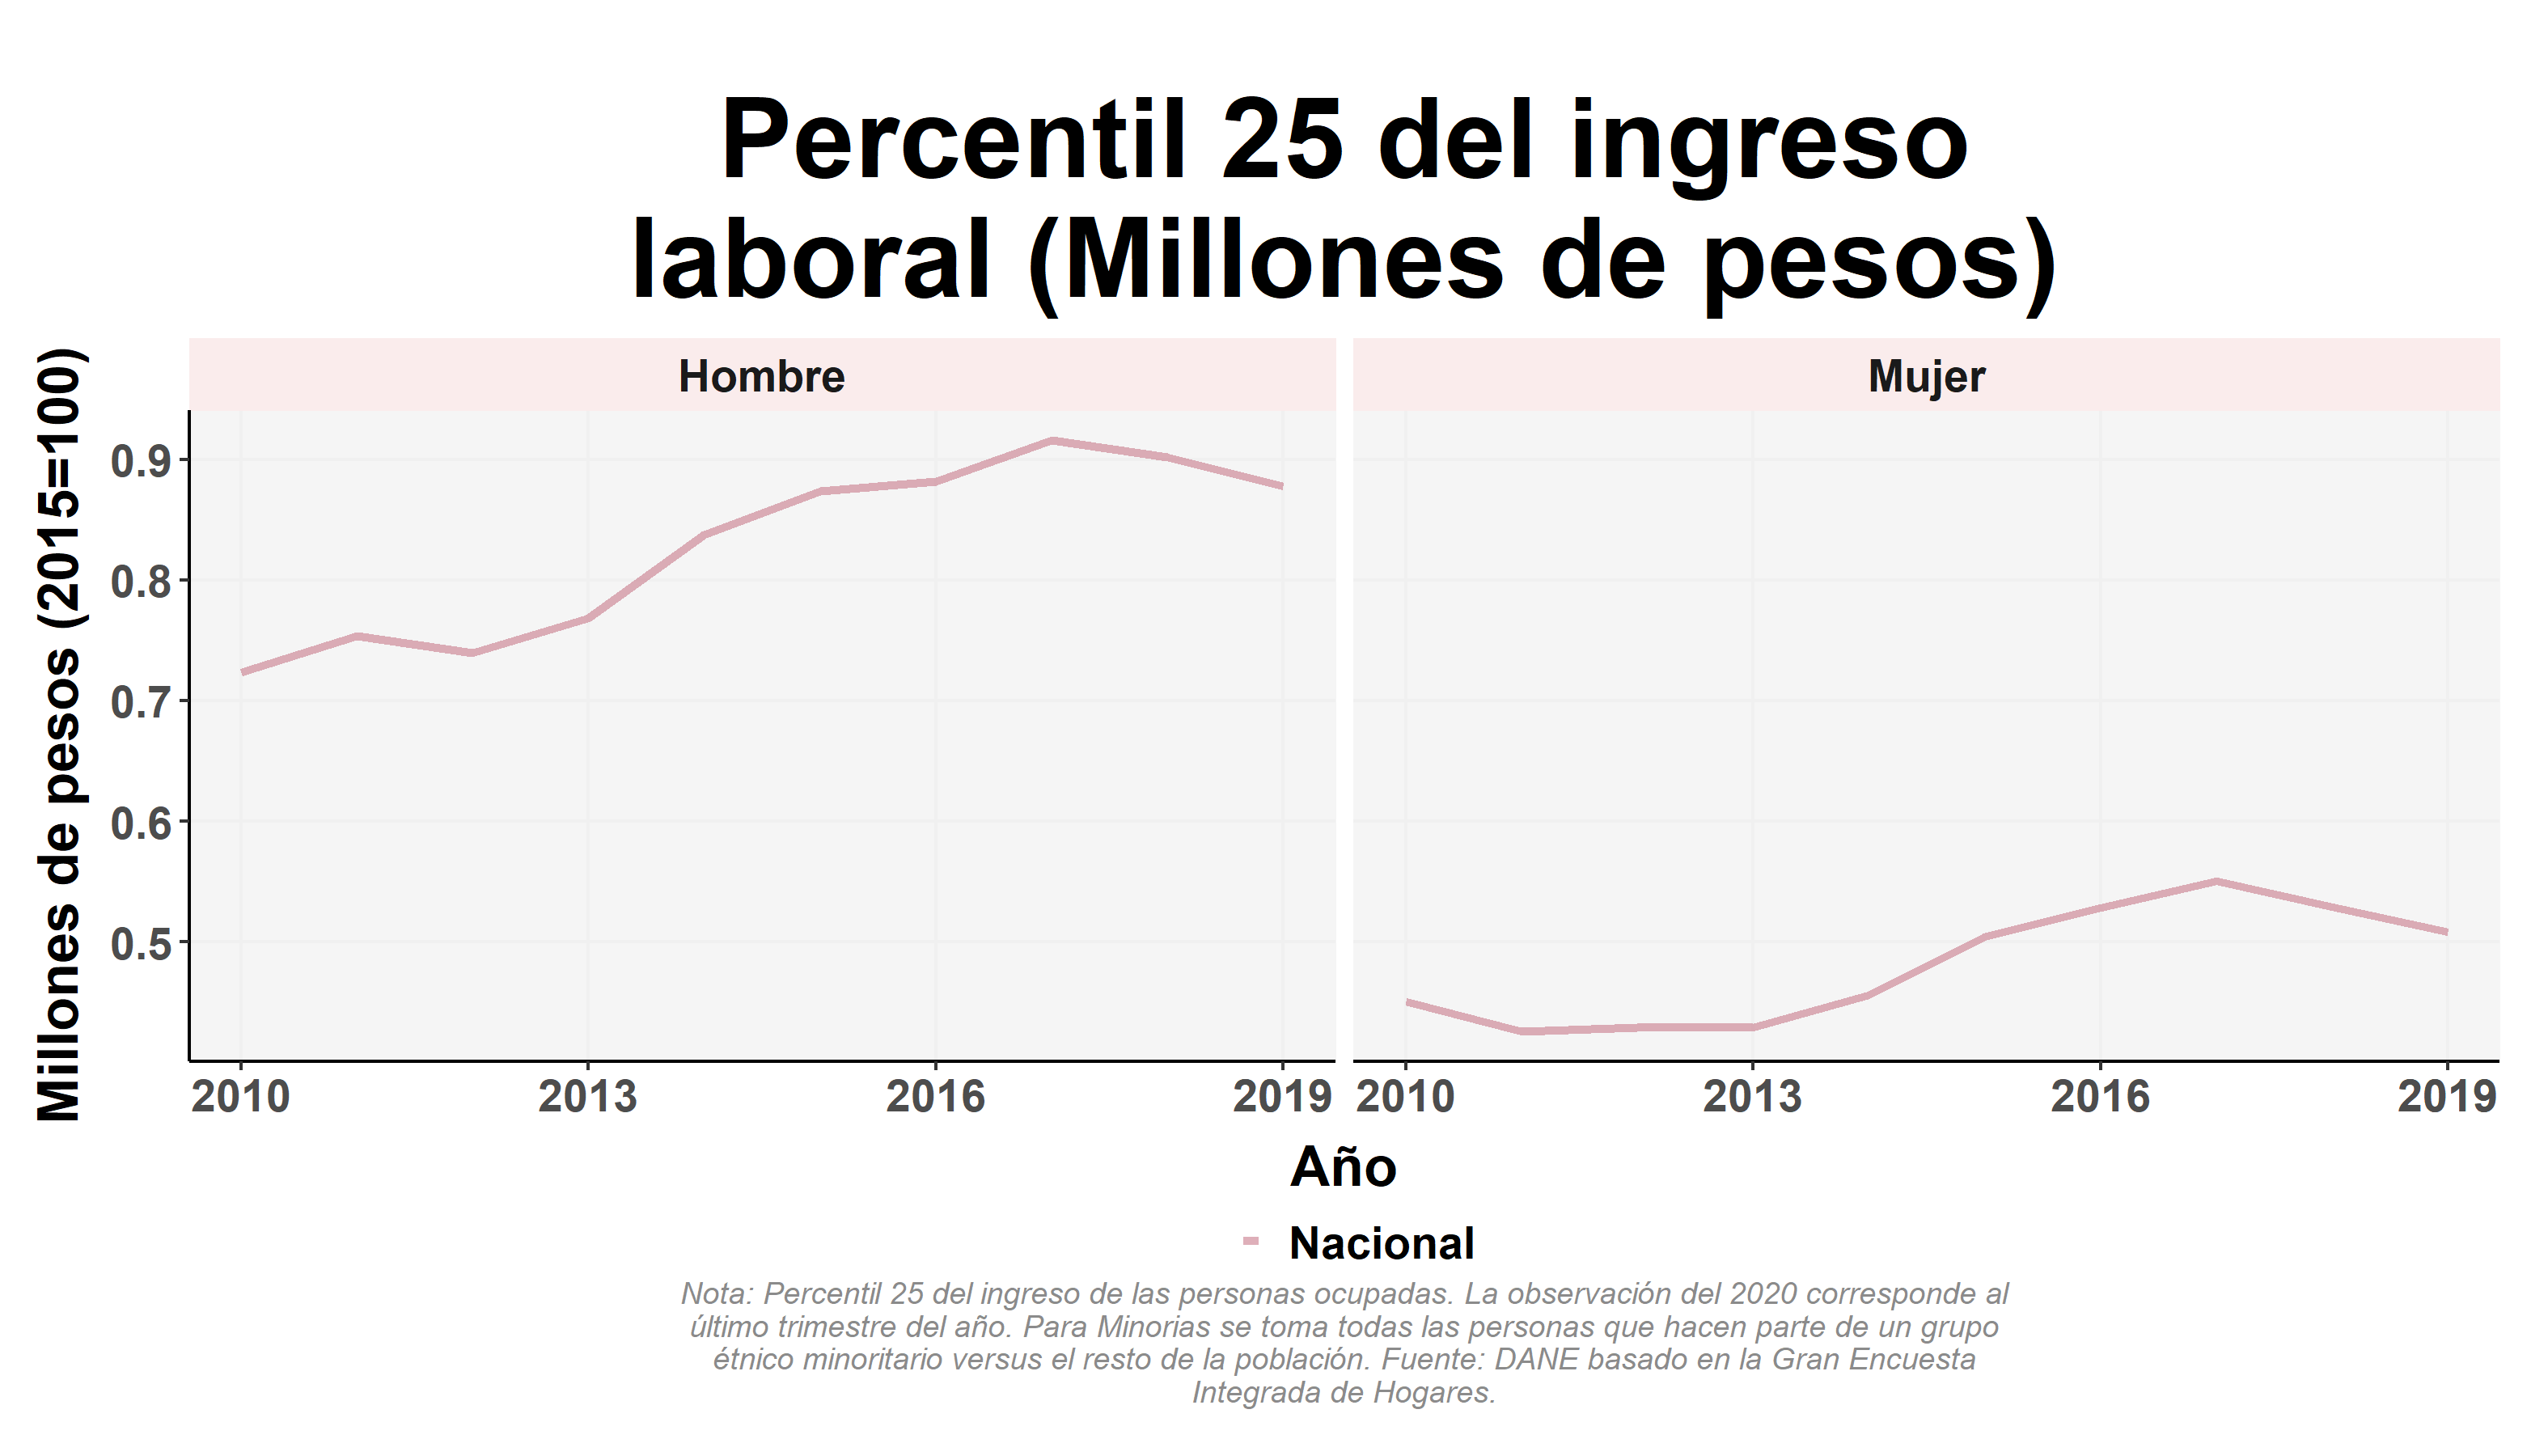
\includegraphics[width=\textwidth,keepaspectratio]{img/var_4_trend.png}
        \end{center}
    \end{figure}
            \begin{itemize}
                    \item Brecha enorme en el ingreso por género en el percentil más bajo, una mujer en el 2019 gana mucho menos que un hombre lo hacía en el 2010.
                    \item Los ingresos estaban aumentando hasta el 2017, pero el del hombre lo hacia de manera más contante que el de la mujer.
                    \item El ingreso venía disminuyendo desde el 2018, y se incentiva más en el 2020 con el Covid. Esto también de ve en el ámbito nacional.
                \end{itemize}

%%%% Include figures
    \begin{figure}[H]
        \caption{Percentil 50 del ingreso laboral por ciudades principales para minorías - 2020 \label{map_result_2} }
        \begin{center}
        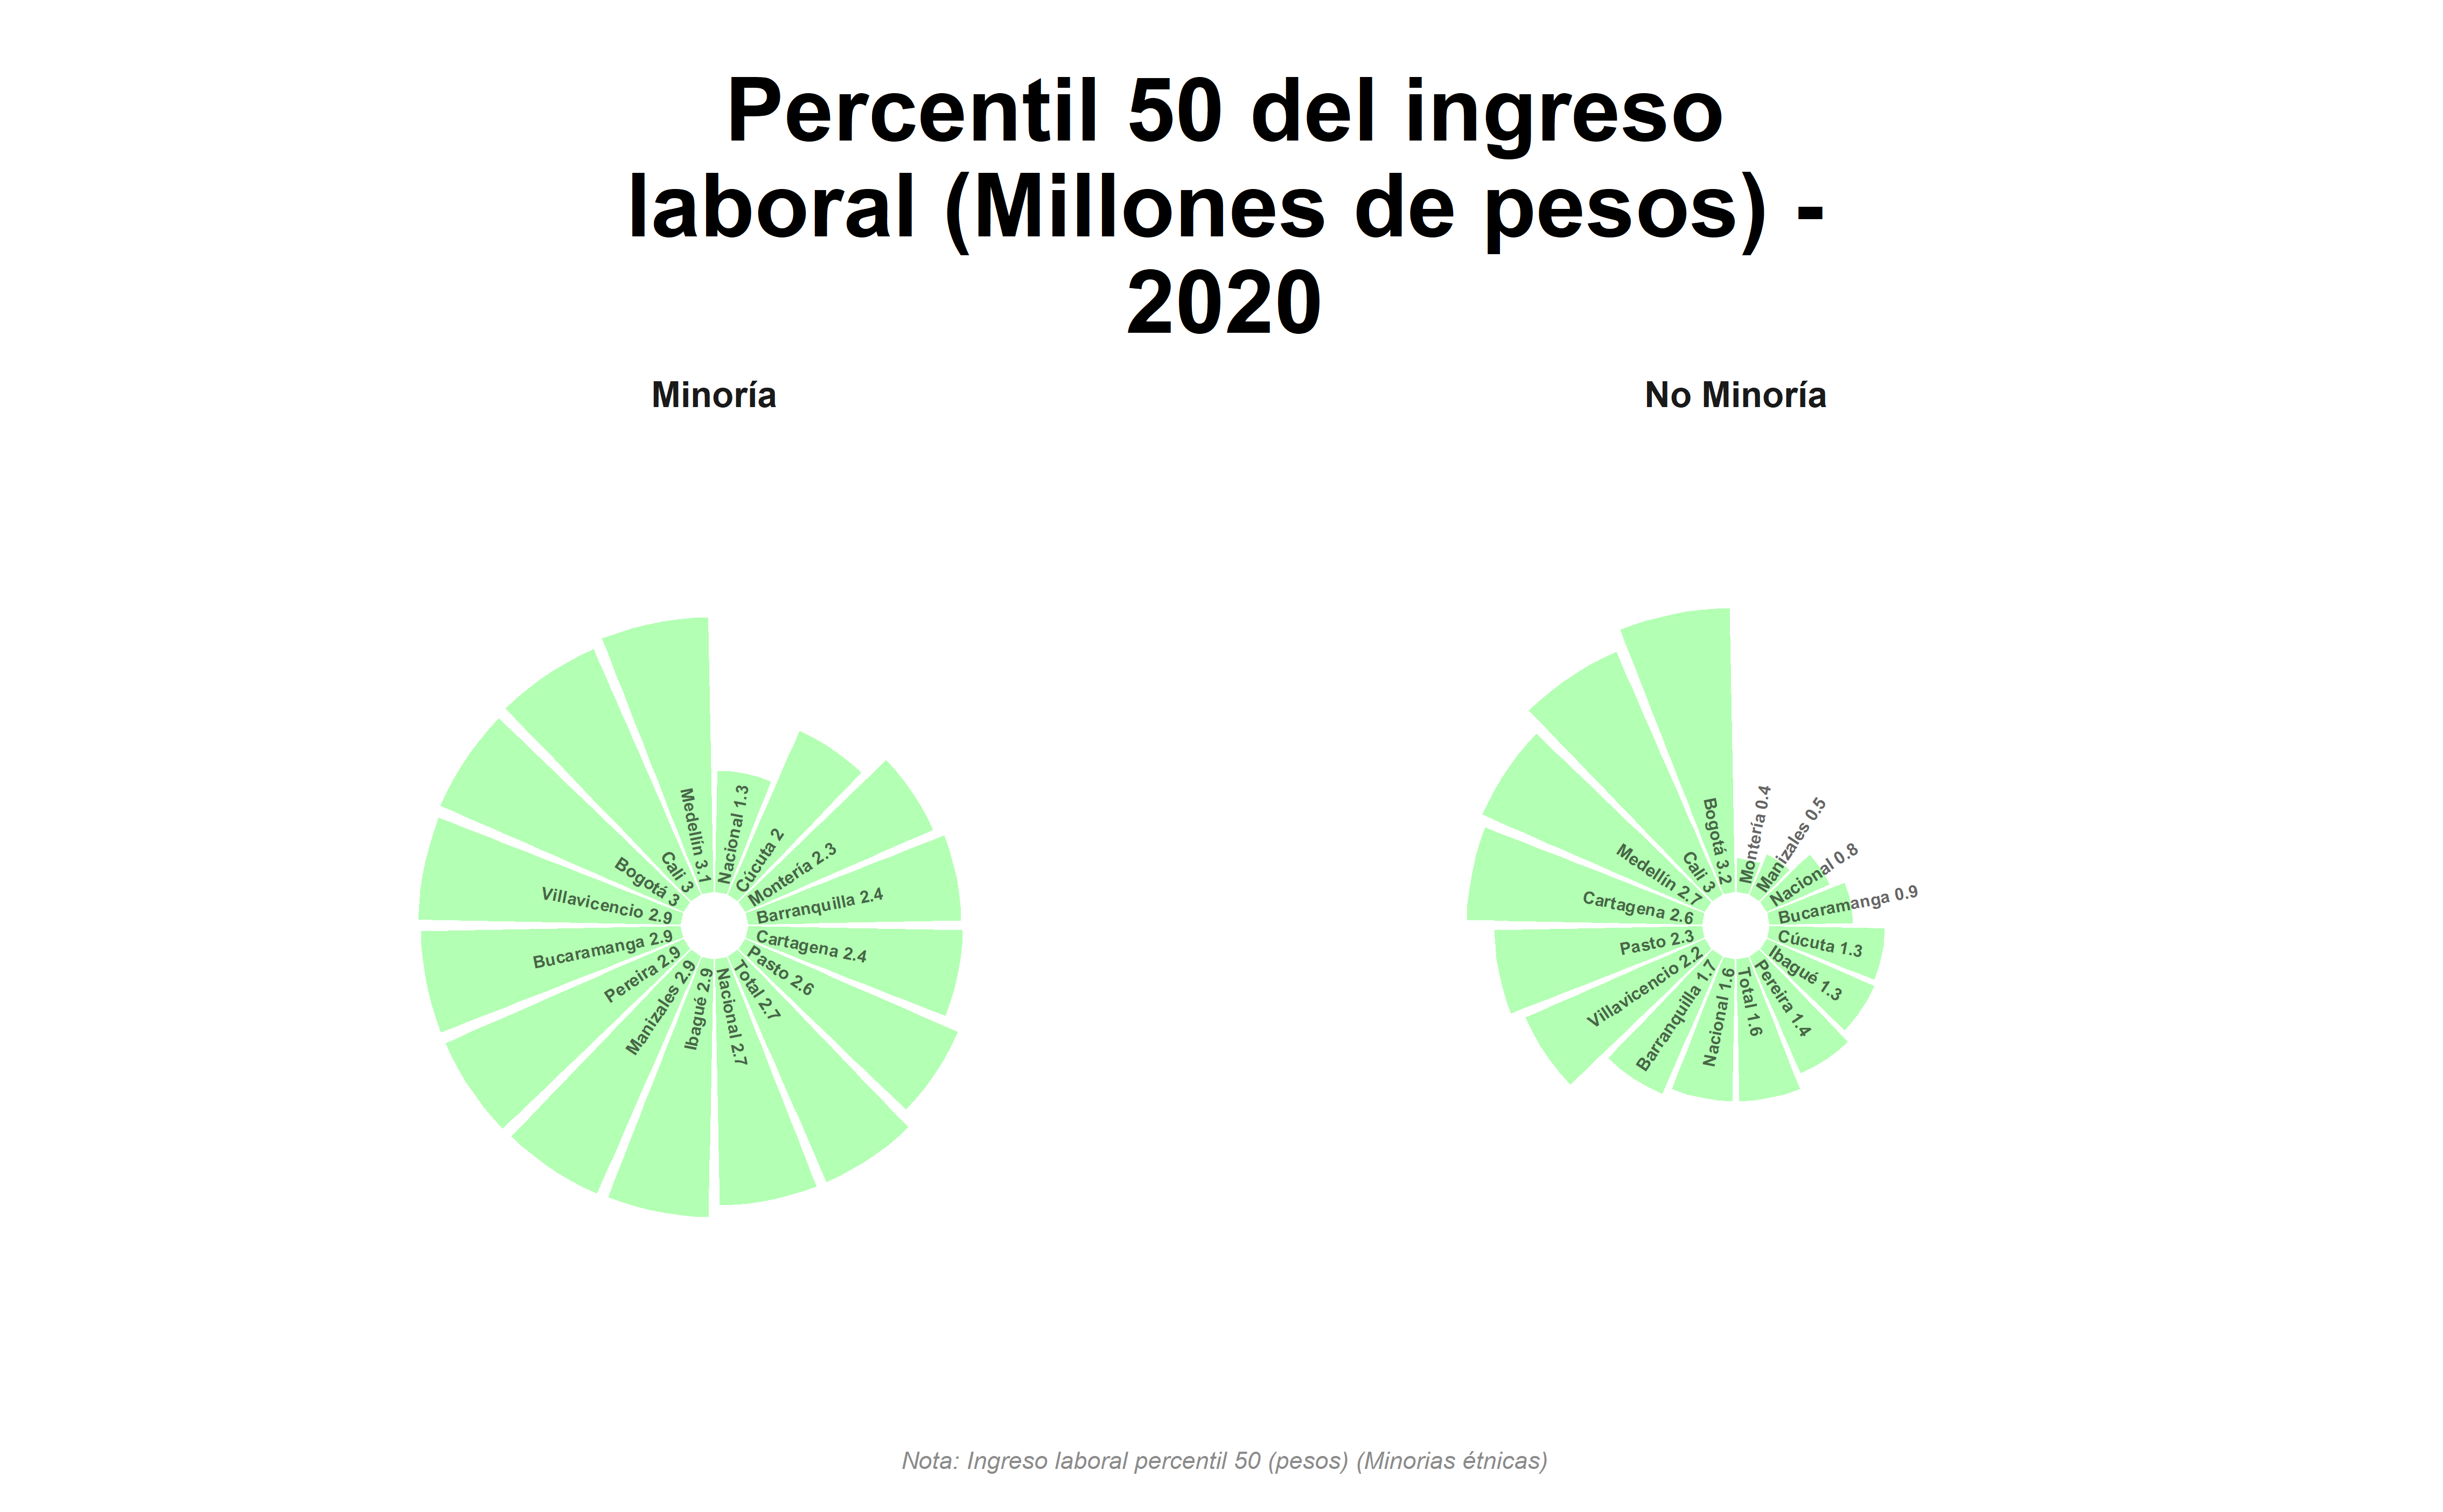
\includegraphics[width=\textwidth,keepaspectratio]{img/var_14_static.png}
        \end{center}
    \end{figure}
            \begin{itemize}
                    \item Diferencia en el ingreso medio de poco más de un millón entre ciudades para minorías (Cúcuta - Medellín), y cerca de tres millones para las no minorías (Montería - Bogotá).
                    \item El ingreso medio nacional es mayor para las no minorías, mismo comportamiento con  Bogotá y Cartagena, mientras que las otras sigue siendo mayor en las minorías.
                    \item El ingreso medio en el caso de las minorías se ve más equitativo que el de las no minorías.
                \end{itemize}

%%%% Include figures
    \begin{figure}[H]
        \caption{Percentil 50 del ingreso laboral por género \label{map_result_2} }
        \begin{center}
        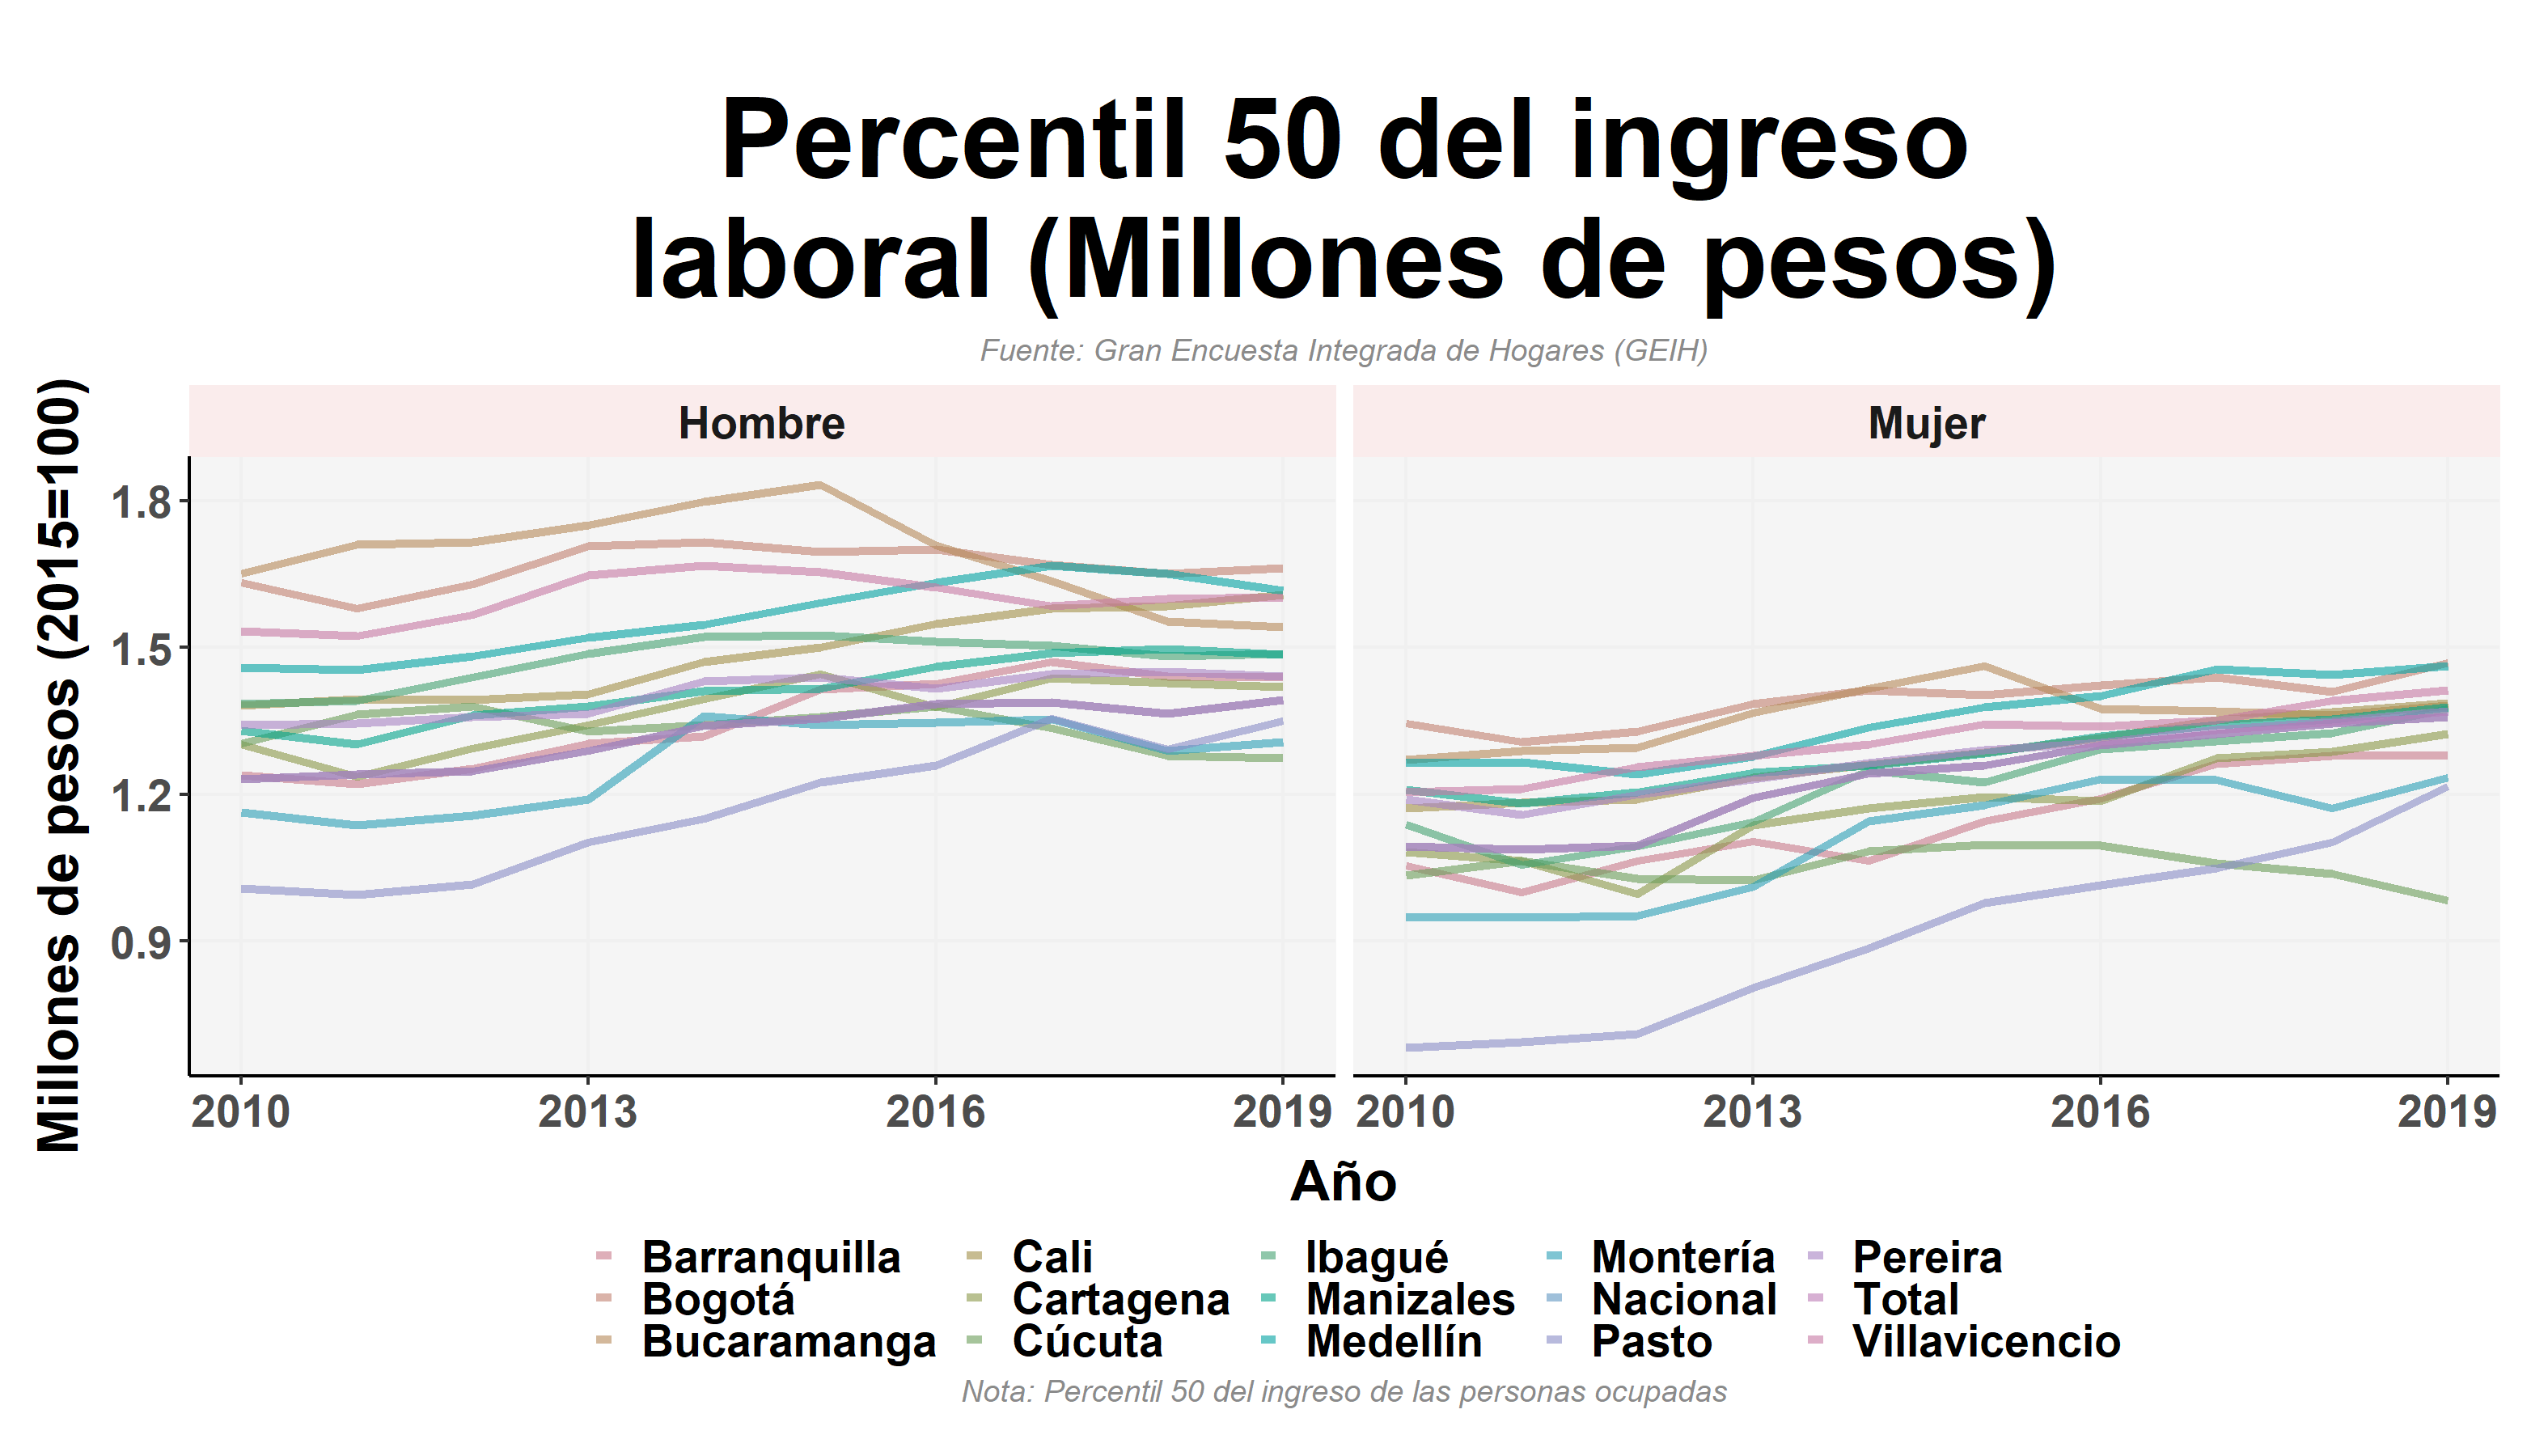
\includegraphics[width=\textwidth,keepaspectratio]{img/var_16_trend.png}
        \end{center}
    \end{figure}
            \begin{itemize}
                    \item El ingreso por género en el percentil 50 tiene menos diferencia a comparación como en el percentil 25.
                    \item La diferencia entre géneros muestra que hace 10 años era más de cien mil y ahora es menor.
                    \item El ingreso de la mujer ha aumentado de manera constante desde el 2012, mientras que el del hombre se ha mantenido igual desde el 2016, con una caída en el 2018.
                    \item Los ingresos por género en el percentil 50 han mejorado con el tiempo, de igual manera se ve que lo ha hecho el total nacional.
                \end{itemize}

%%%% Include figures
    \begin{figure}[H]
        \caption{Percentil 75 del ingreso laboral por ciudades principales para minorías - 2020 \label{map_result_2} }
        \begin{center}
        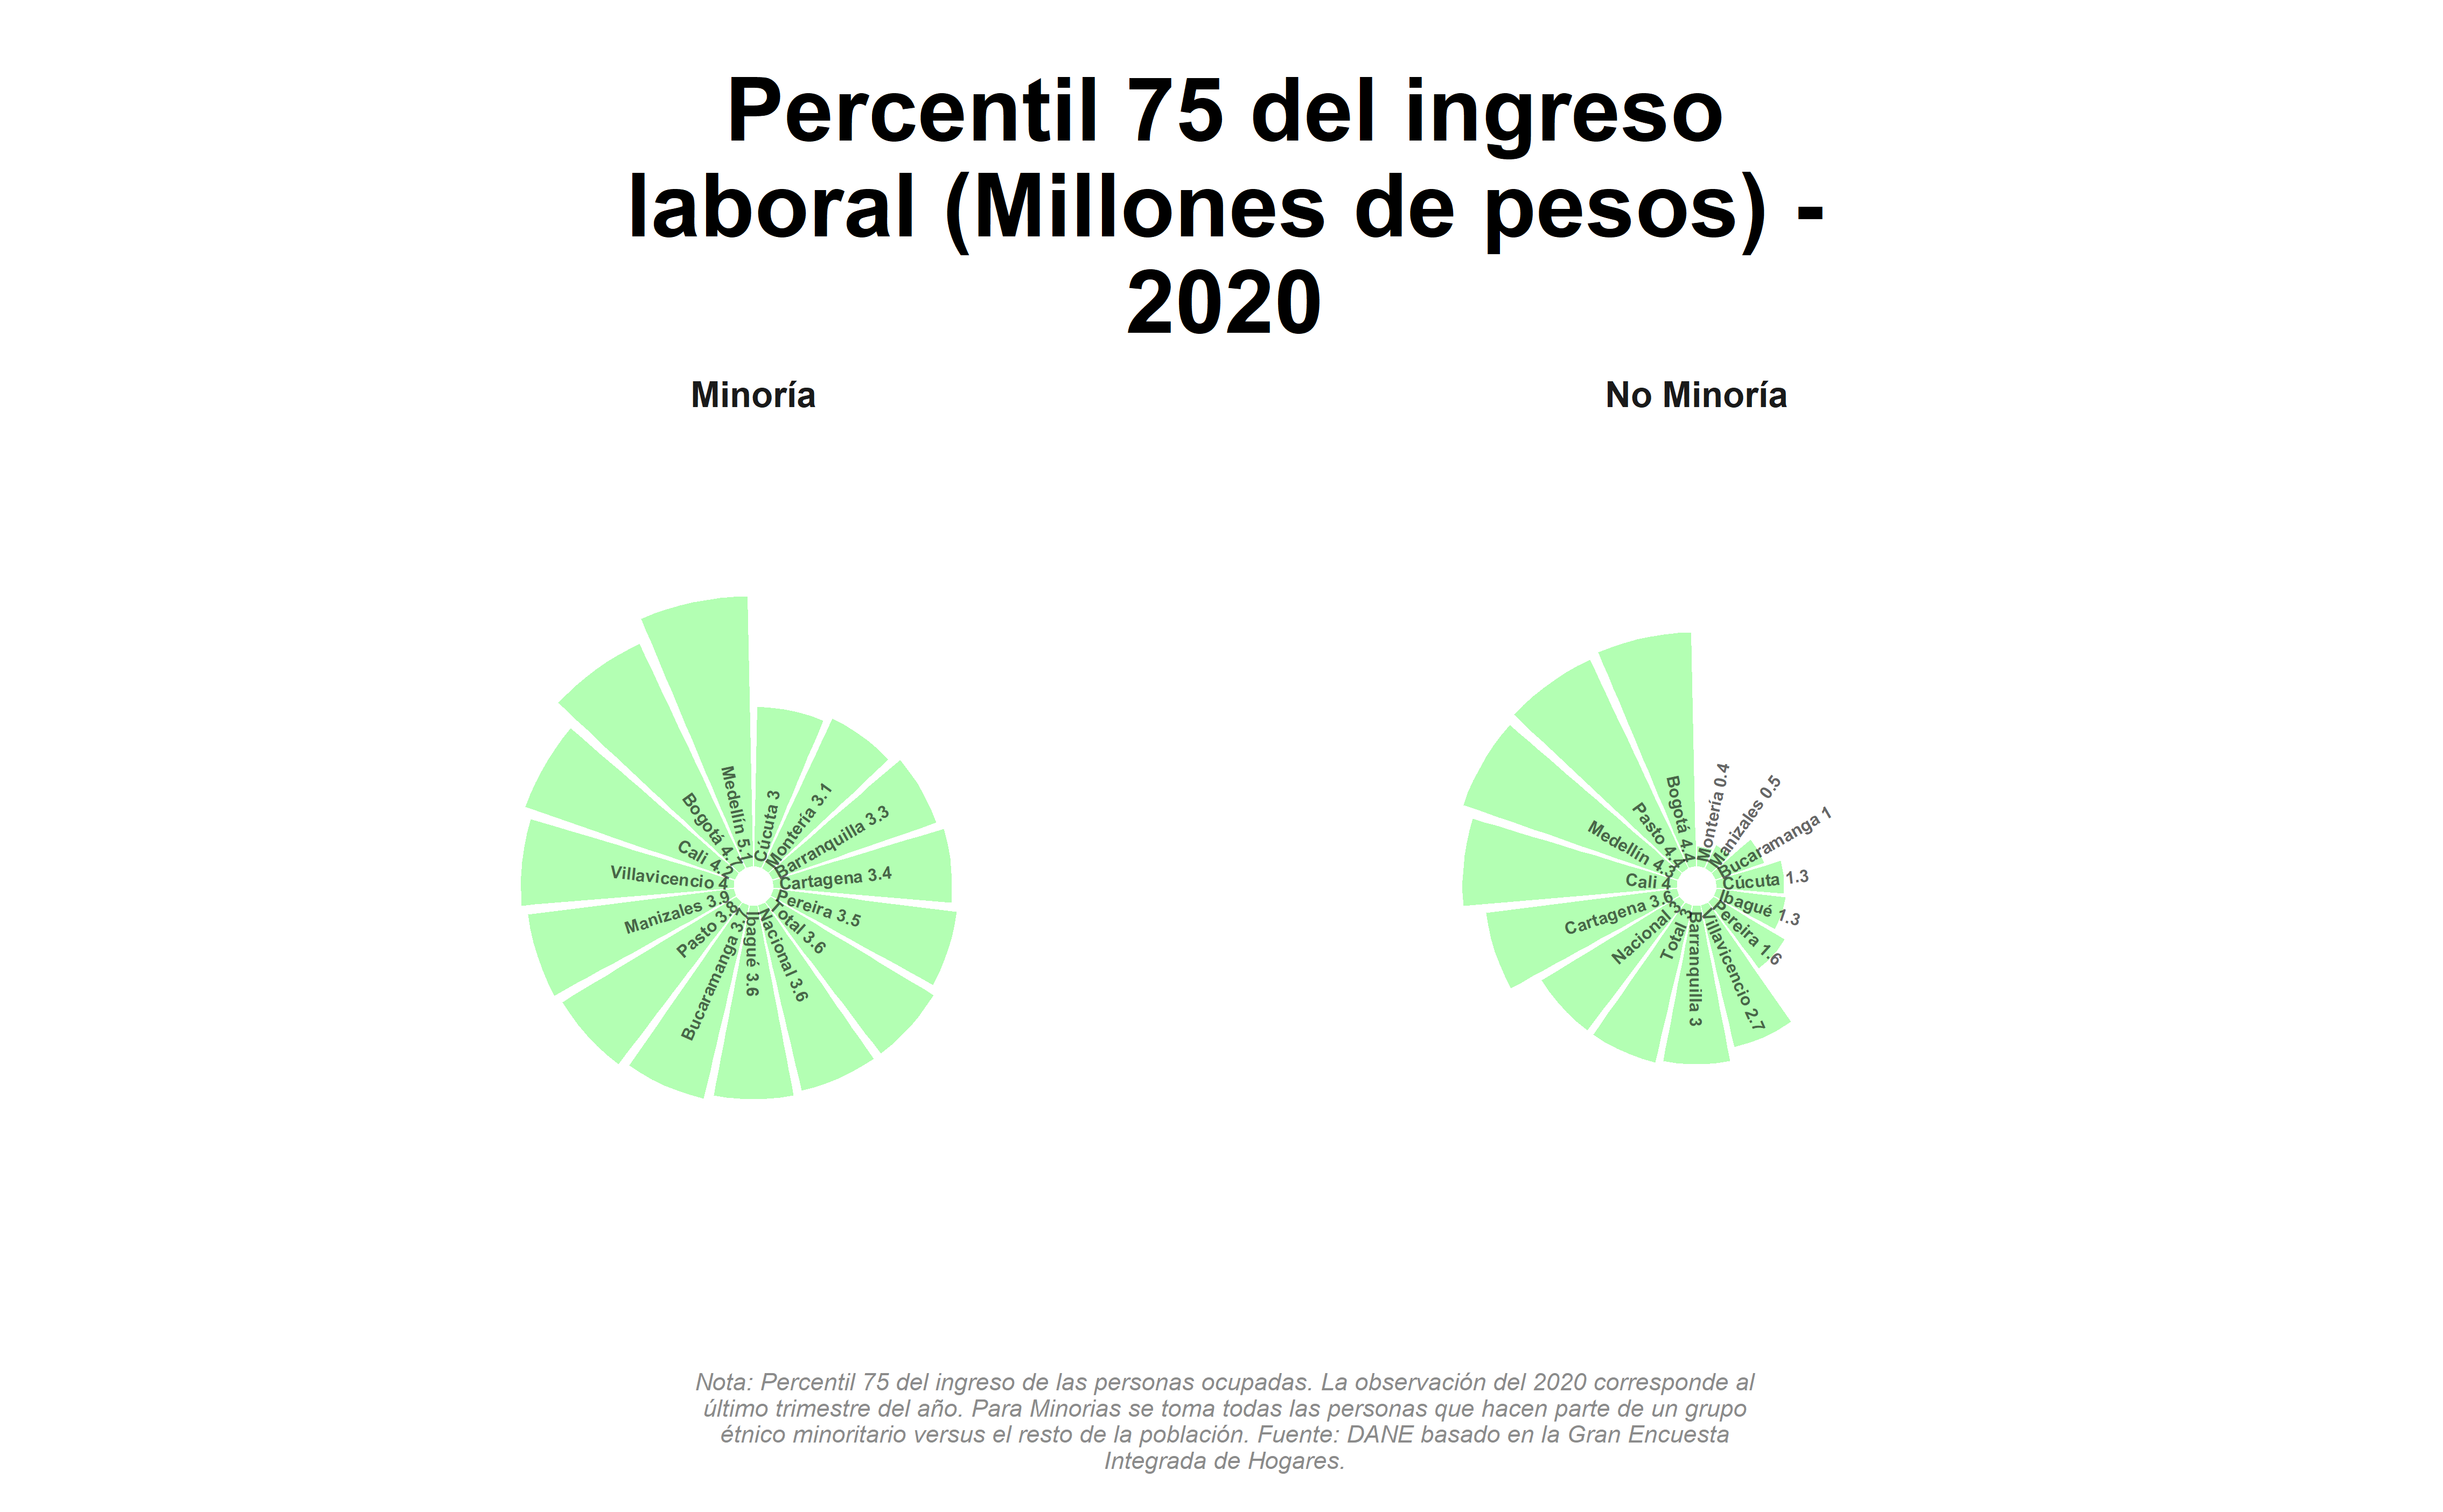
\includegraphics[width=\textwidth,keepaspectratio]{img/var_24_static.png}
        \end{center}
    \end{figure}
            \begin{itemize}
                    \item Diferencia en el ingreso medio entre las ciudades extremos es de dos millones para minorías (Cúcuta - Medellín), y cerca de cuatro millones para las no minorías (Montería - Bogotá).
                    \item Solo Cartagena presenta un ingreso medio nacional mayor para las no minorías, el resto tiene el comportamiento contrario, incluido a nivel nacional.
                    \item Al igual que en el percentil 50, el ingreso medio de las minorías se ve más equitativo que el de las no minorías.
                \end{itemize}

%%%% Include figures
    \begin{figure}[H]
        \caption{Percentil 75 del ingreso laboral por género \label{map_result_2} }
        \begin{center}
        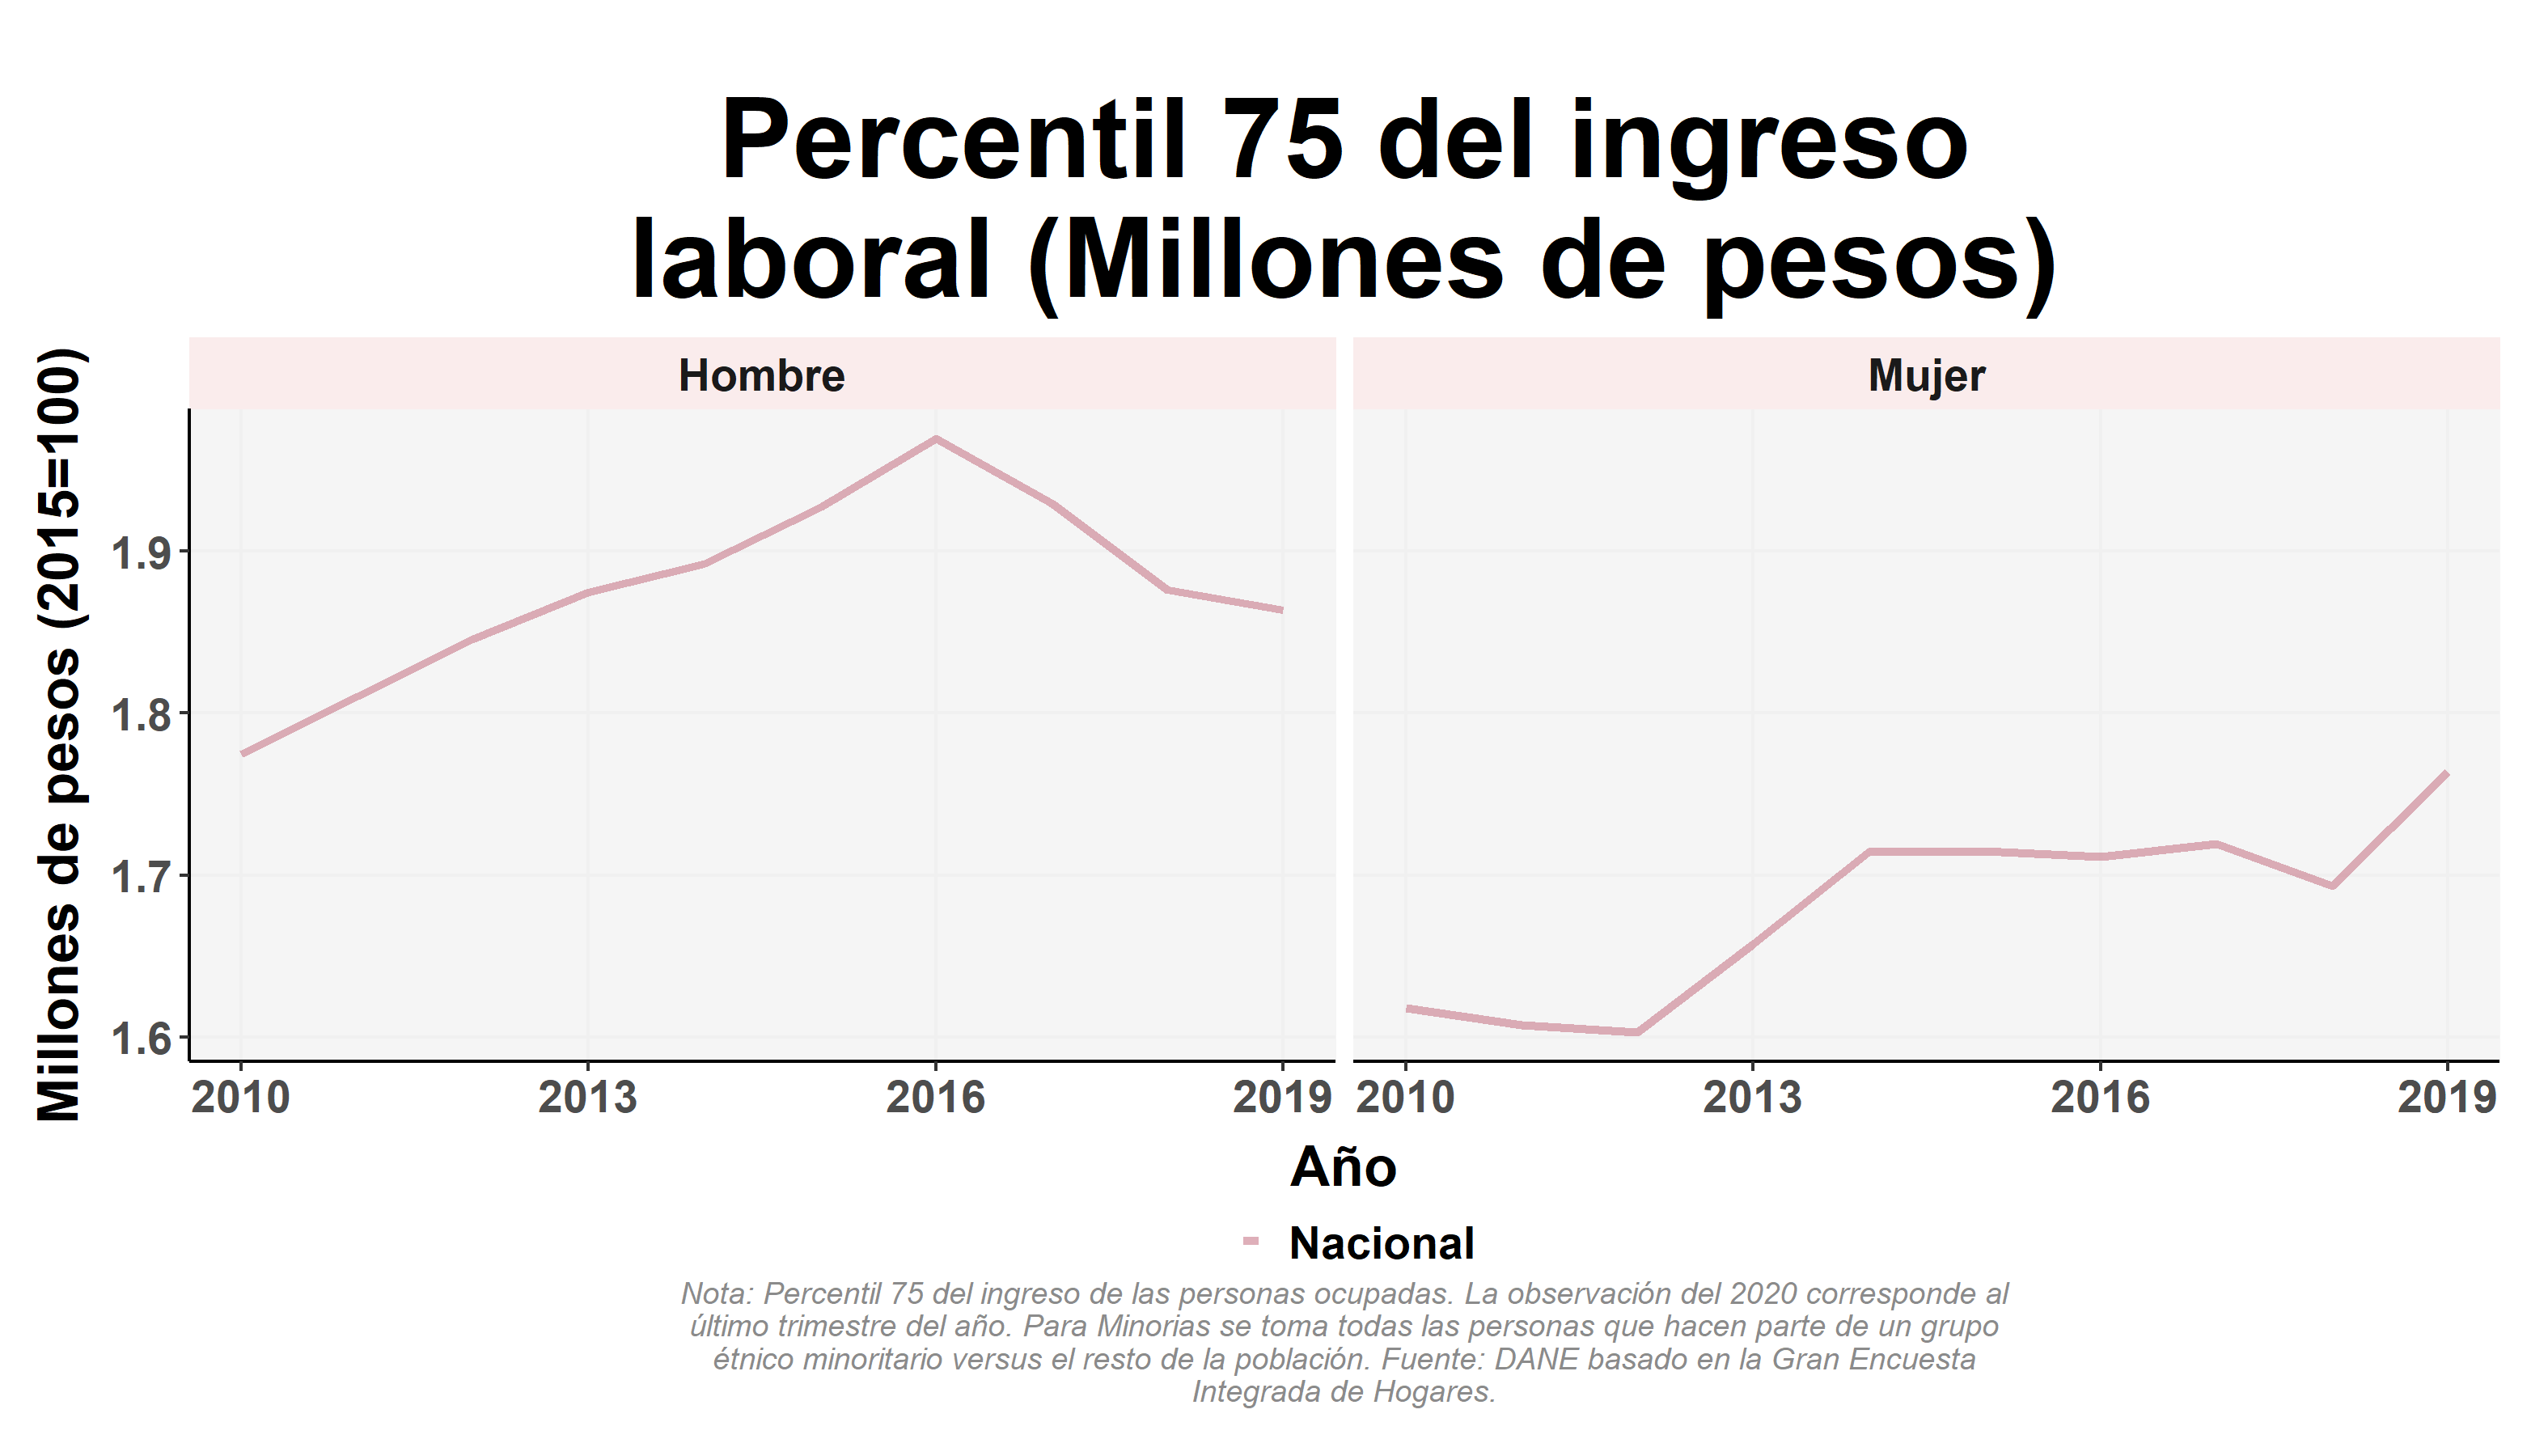
\includegraphics[width=\textwidth,keepaspectratio]{img/var_26_trend.png}
        \end{center}
    \end{figure}
            \begin{itemize}
                    \item En el percentil 75 la brecha de ingreso medio entre géneros ha disminuido, pero aún es persistente, siendo la mujer de menor ingreso.
                    \item El ingreso medio de los hombres en el percentil 75 ha venido disminuyendo desde el 2016.
                    \item En el caso de la mujer el ingreso no ha aumentado significativamente, manteniendo el ingreso en 2019 igual al percibido por un hombre en 2010.
                \end{itemize}

%%%% Include figures
    \begin{figure}[H]
        \caption{Percentil 75 del ingreso laboral nacional \label{map_result_2} }
        \begin{center}
        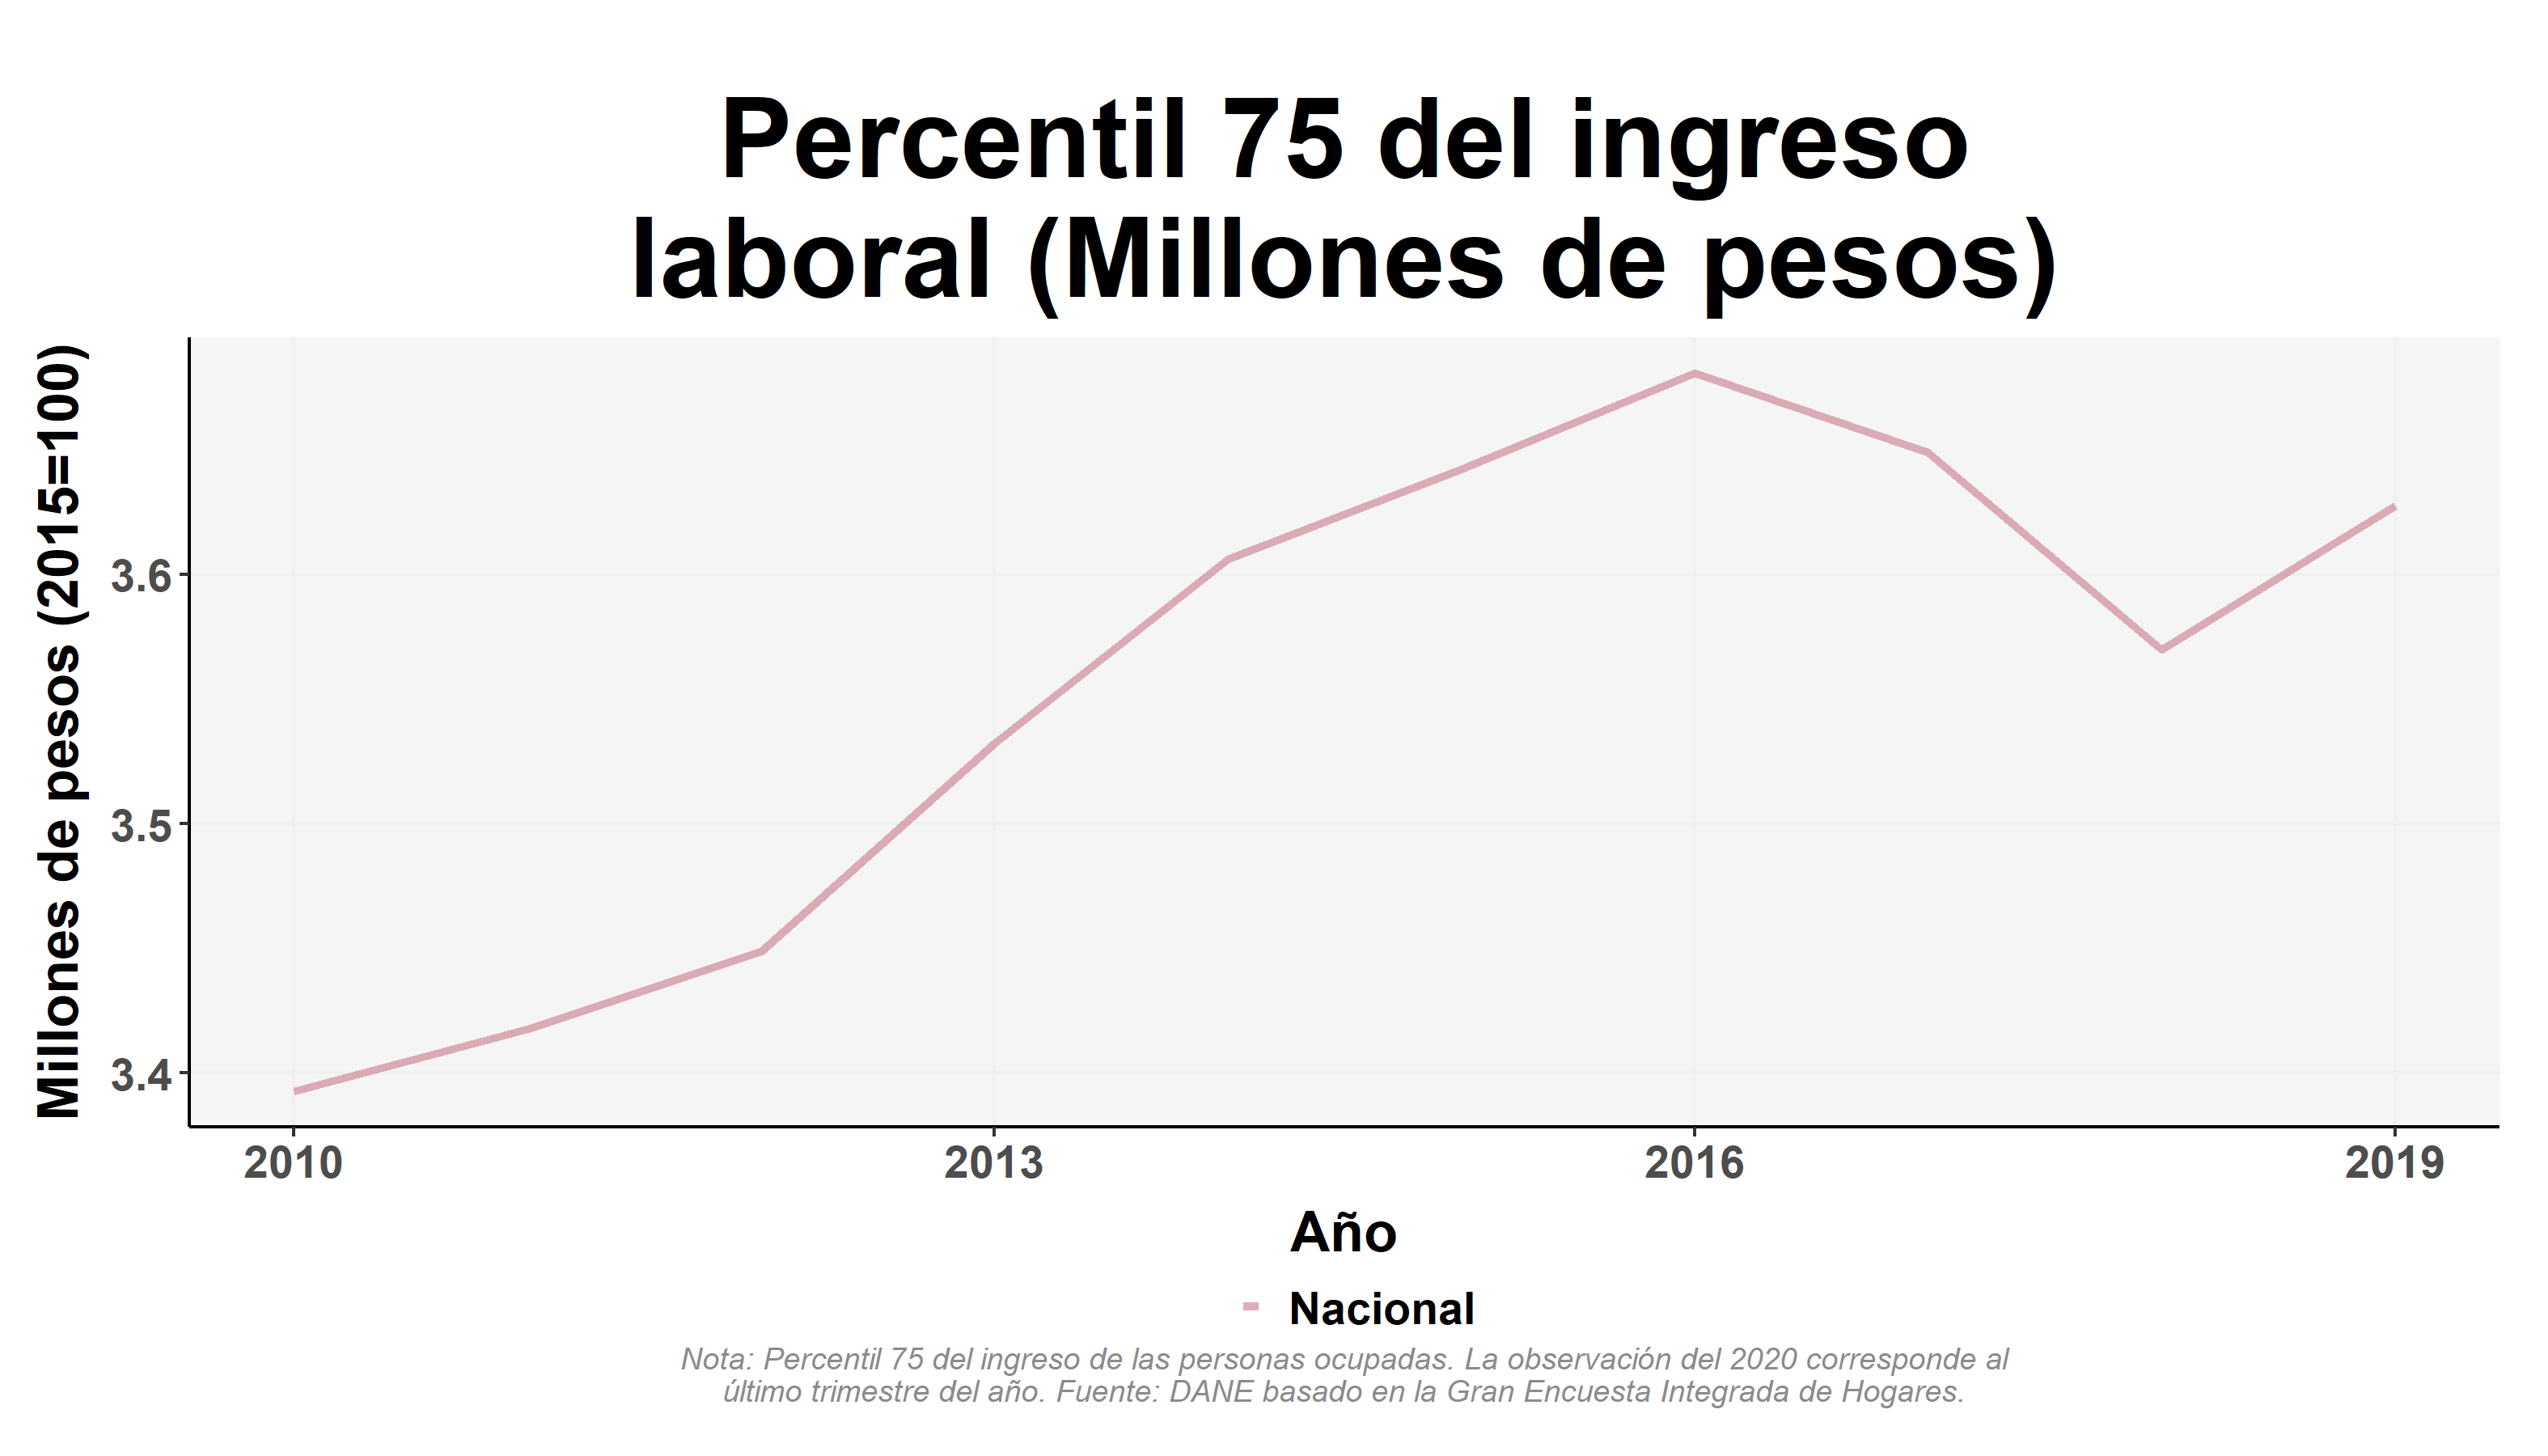
\includegraphics[width=\textwidth,keepaspectratio]{img/var_27_trend.png}
        \end{center}
    \end{figure}
            \begin{itemize}
                    \item El ingreso medio nacional en el percentil 75 tuvo crecimiento constante hasta el 2016 donde empezó a disminuir hasta el 2017 donde vuelve a verse un aumento para el 2019.
                    \item Este comportamiento se asemeja al de los hombres para el percentil 75.
                \end{itemize}

\section{Pobreza}
    \subsection{Pobreza Monetaria}
        \subsubsection{Población por Clase Social}

%%%% Include figures
    \begin{figure}[H]
        \caption{Población por clase social - Pobres (2012 VS 2020) por ciudad \label{map_result_2} }
        \begin{center}
        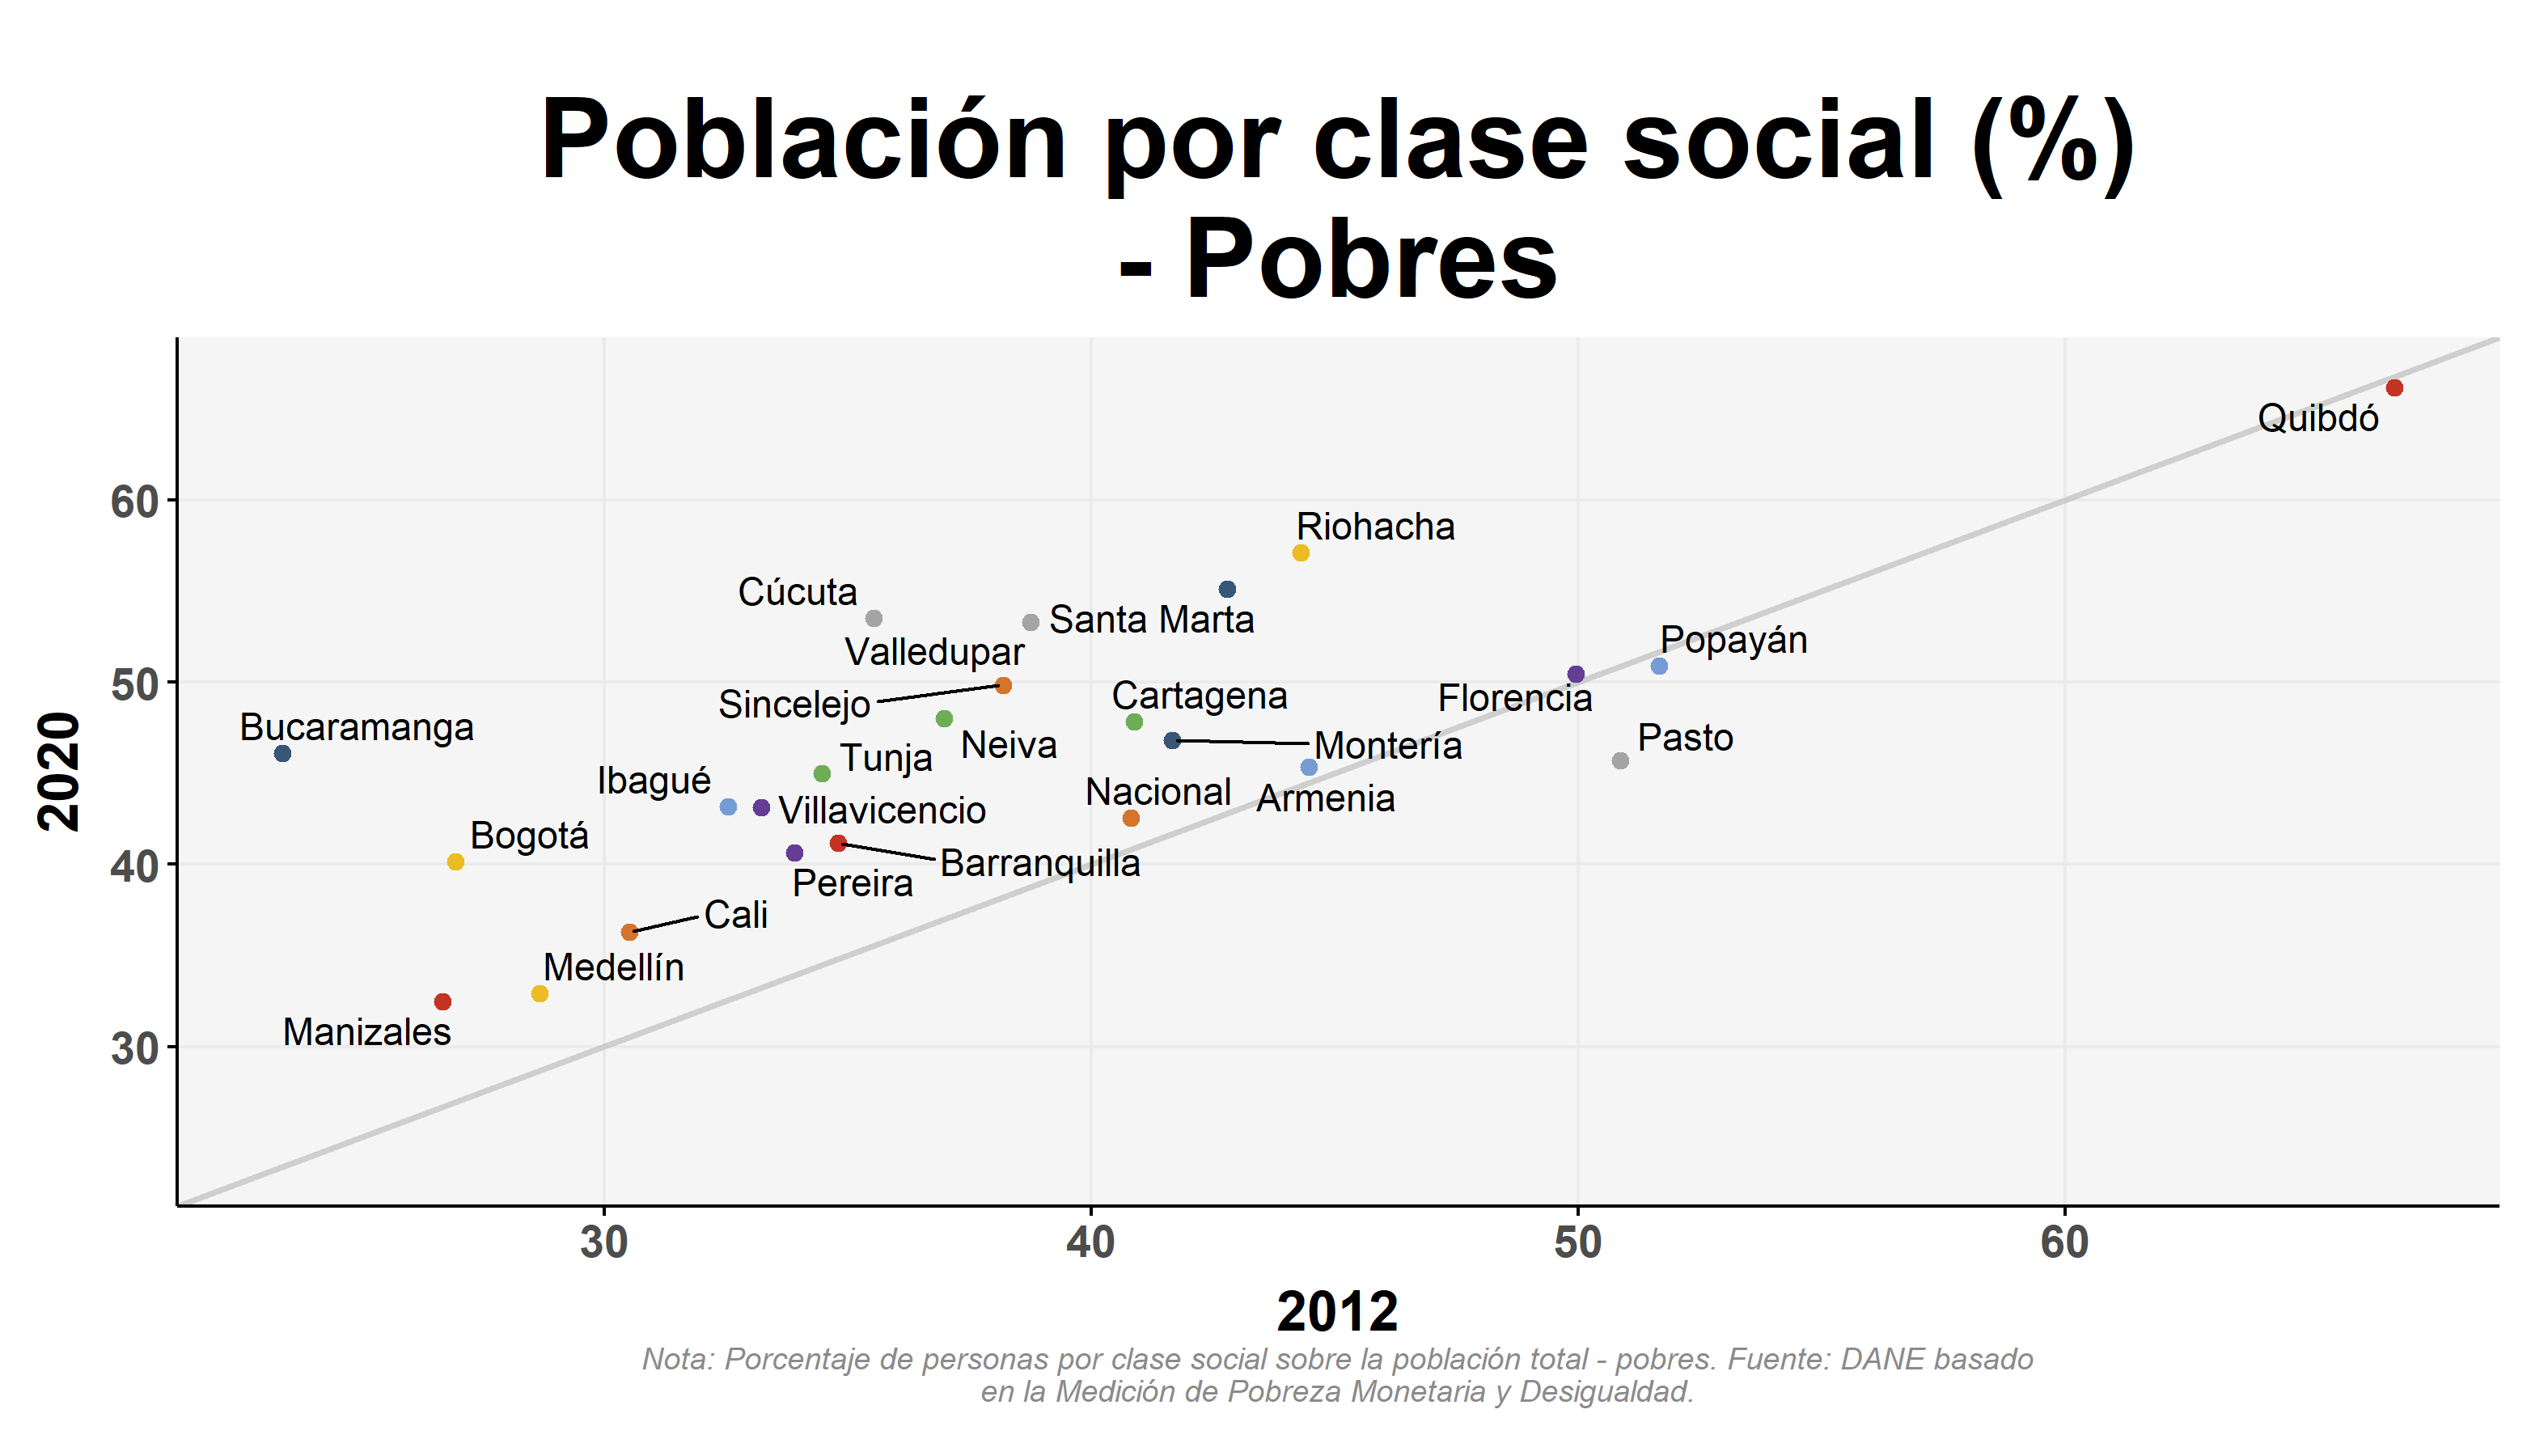
\includegraphics[width=\textwidth,keepaspectratio]{img/var_241_scatter_time.png}
        \end{center}
    \end{figure}
            \begin{itemize}
                    \item Pasto es la única ciudad que disminuyó el porcentaje de pobres entre 2012 y 2020.
                    \item Quibdó, Popayán, Florencia y Armenia mantuvieron el porcentaje de pobres similares entre el 2012 y 2020.
                    \item Gran parte de las ciudades mostraron un aumento en el porcentaje de pobres para el 2020.
                    \item Quibdó sobresale entre las demás ciudades con niveles de pobreza sobre el 60\% y con una diferencia con el segundo de menos del 10\% para 2020, la brecha disminuyó comparado con el 2012 (más del 10\%).
                    \item A nivel nacional la pobreza aumentó levemente.
                    \item Bucaramanga pasó de ser la ciudad con menor porcentaje de pobreza con niveles por debajo del 30\% en 2012 a tener niveles por encima del 45\% para 2020.
                    \item Hay una diferencia de aproximadamente un 30\% entre la ciudad con mayor nivel de pobreza, Quibdó, y la de menor nivel, Manizales, para el 2020 (Se puede evidenciar en el static).
                \end{itemize}

%%%% Include figures
    \begin{figure}[H]
        \caption{Población por clase social - Pobres a nivel nacional \label{map_result_2} }
        \begin{center}
        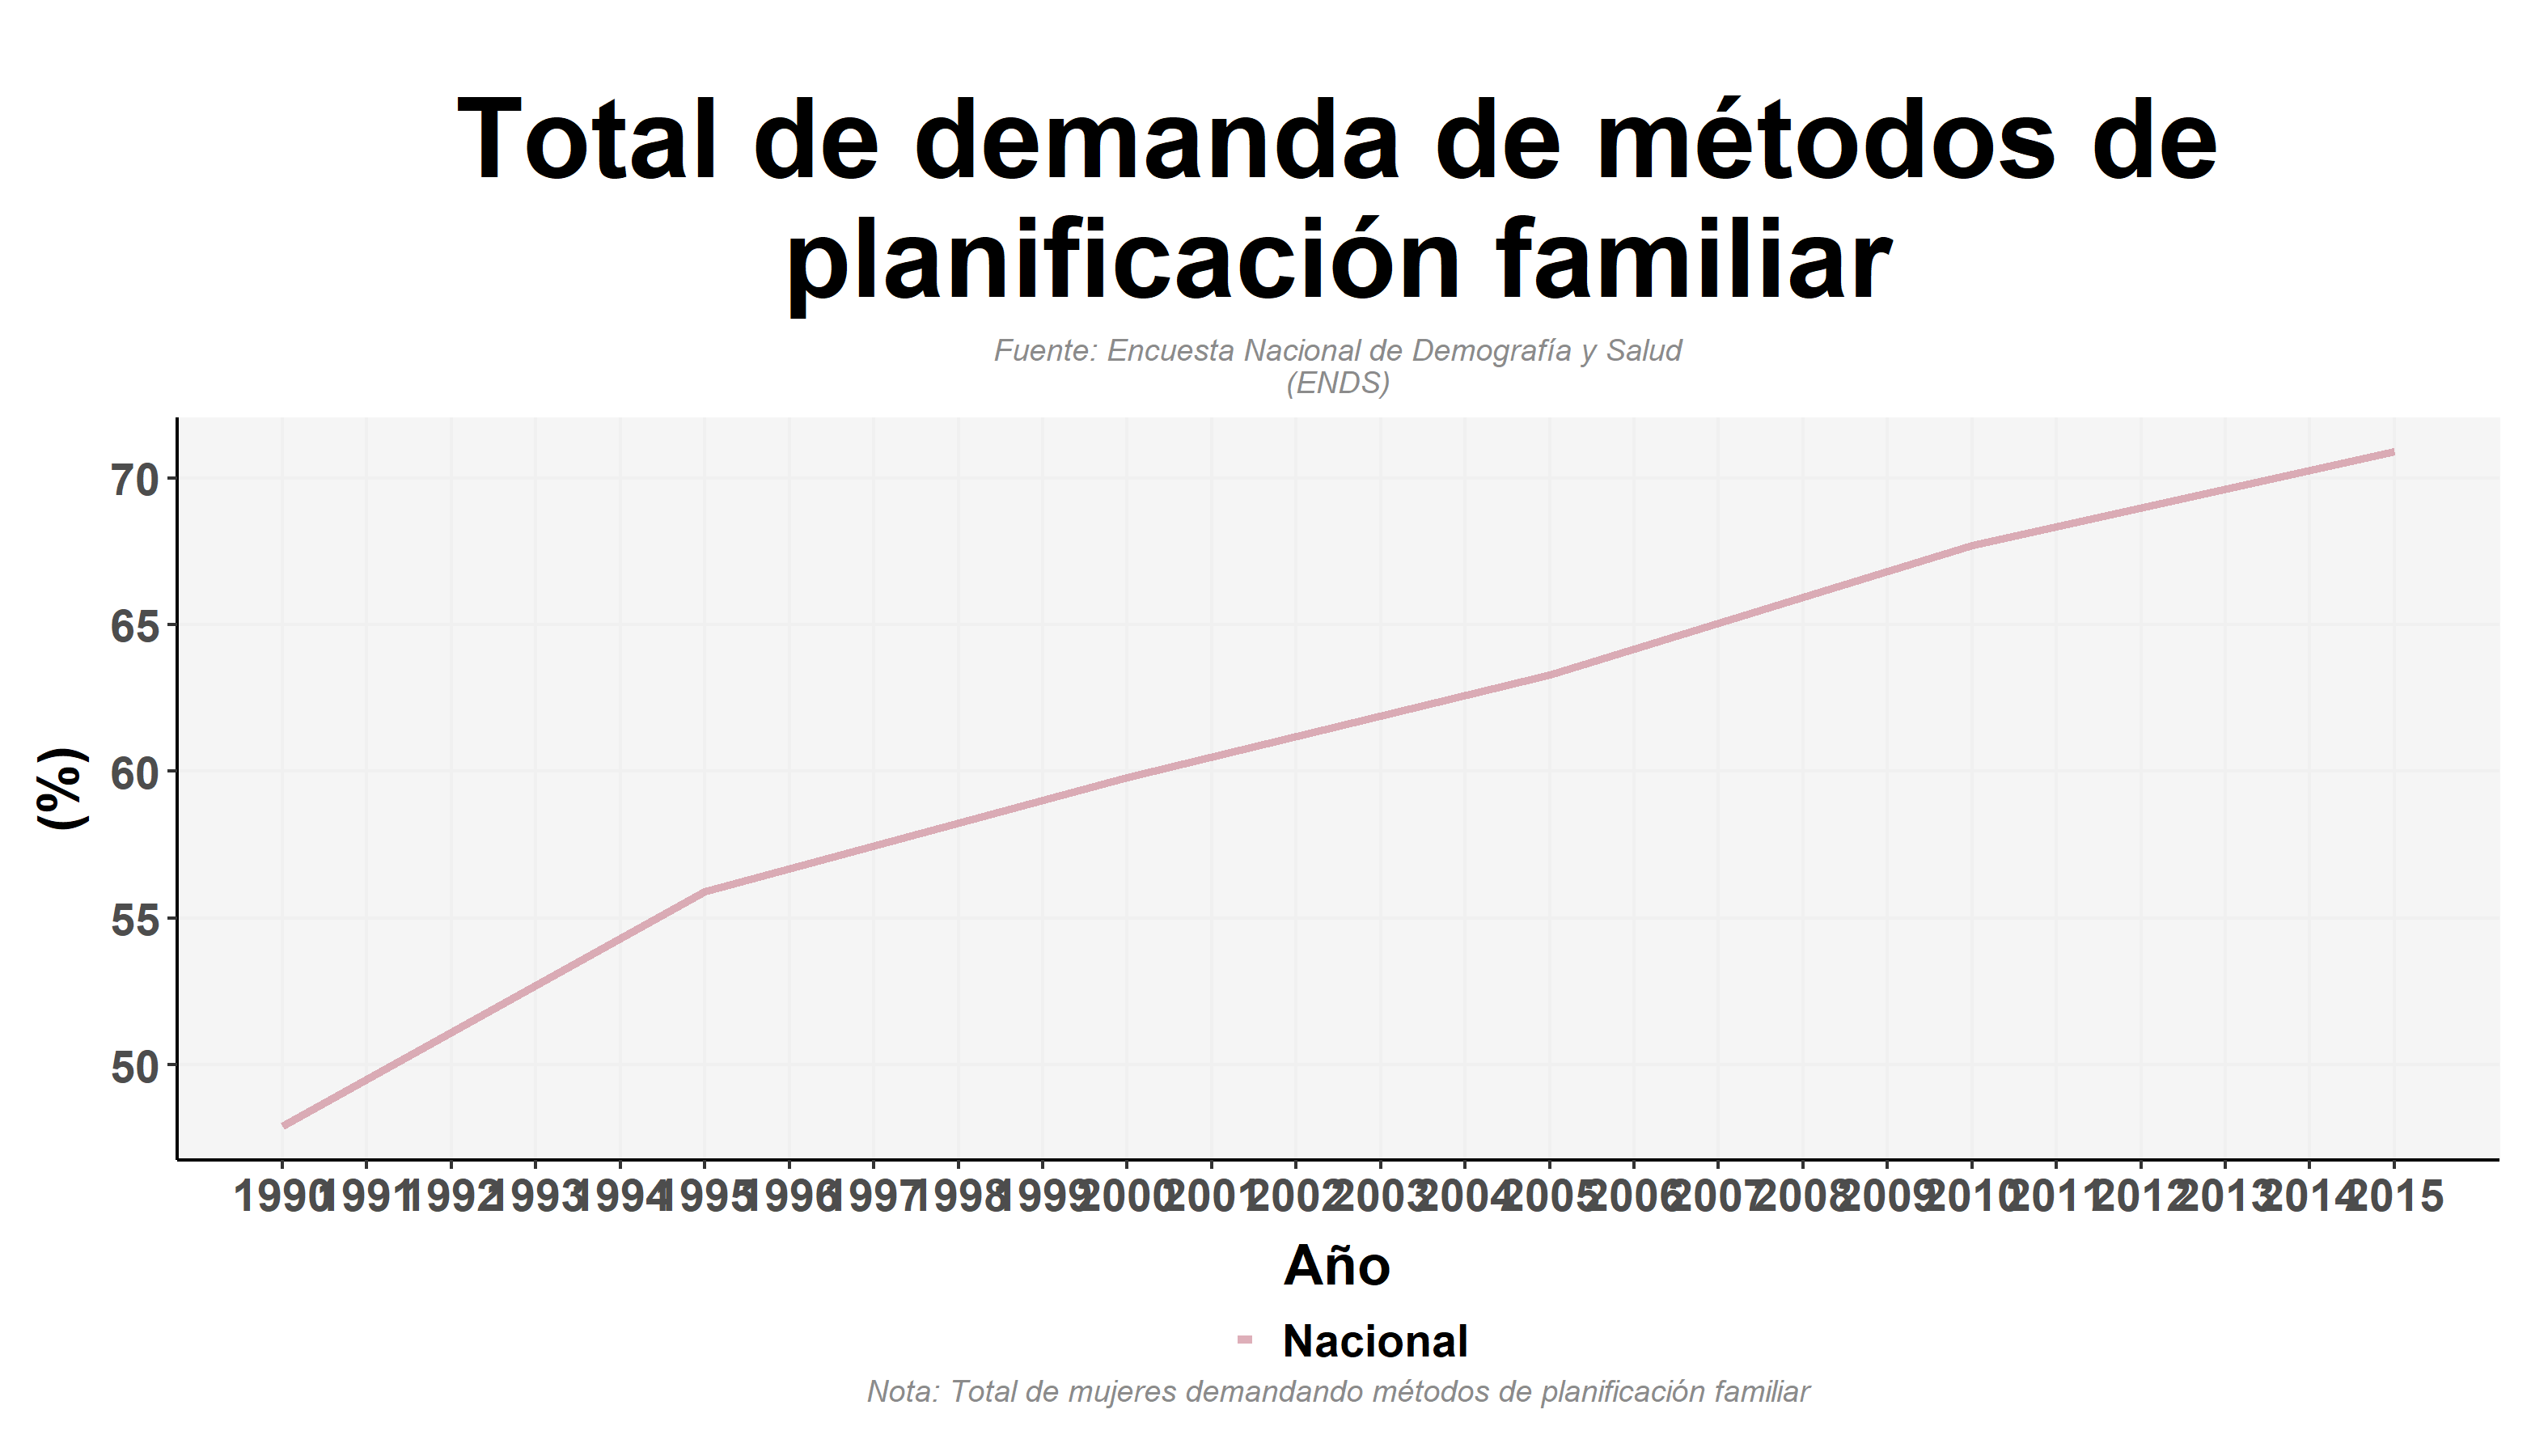
\includegraphics[width=\textwidth,keepaspectratio]{img/var_242_trend.png}
        \end{center}
    \end{figure}
            \begin{itemize}
                    \item El porcentaje de pobres venía disminuyendo a partir del 2012 hasta el 2018, donde empieza a aumentar.
                    \item A partir de 2019 empieza a aumentar el porcentaje de pobreza, y se intensifica en el 2020 superando los niveles del 2012.
                    \end{itemize}

%%%% Include figures
    \begin{figure}[H]
        \caption{Población por clase social - Pobres por zonas \label{map_result_2} }
        \begin{center}
        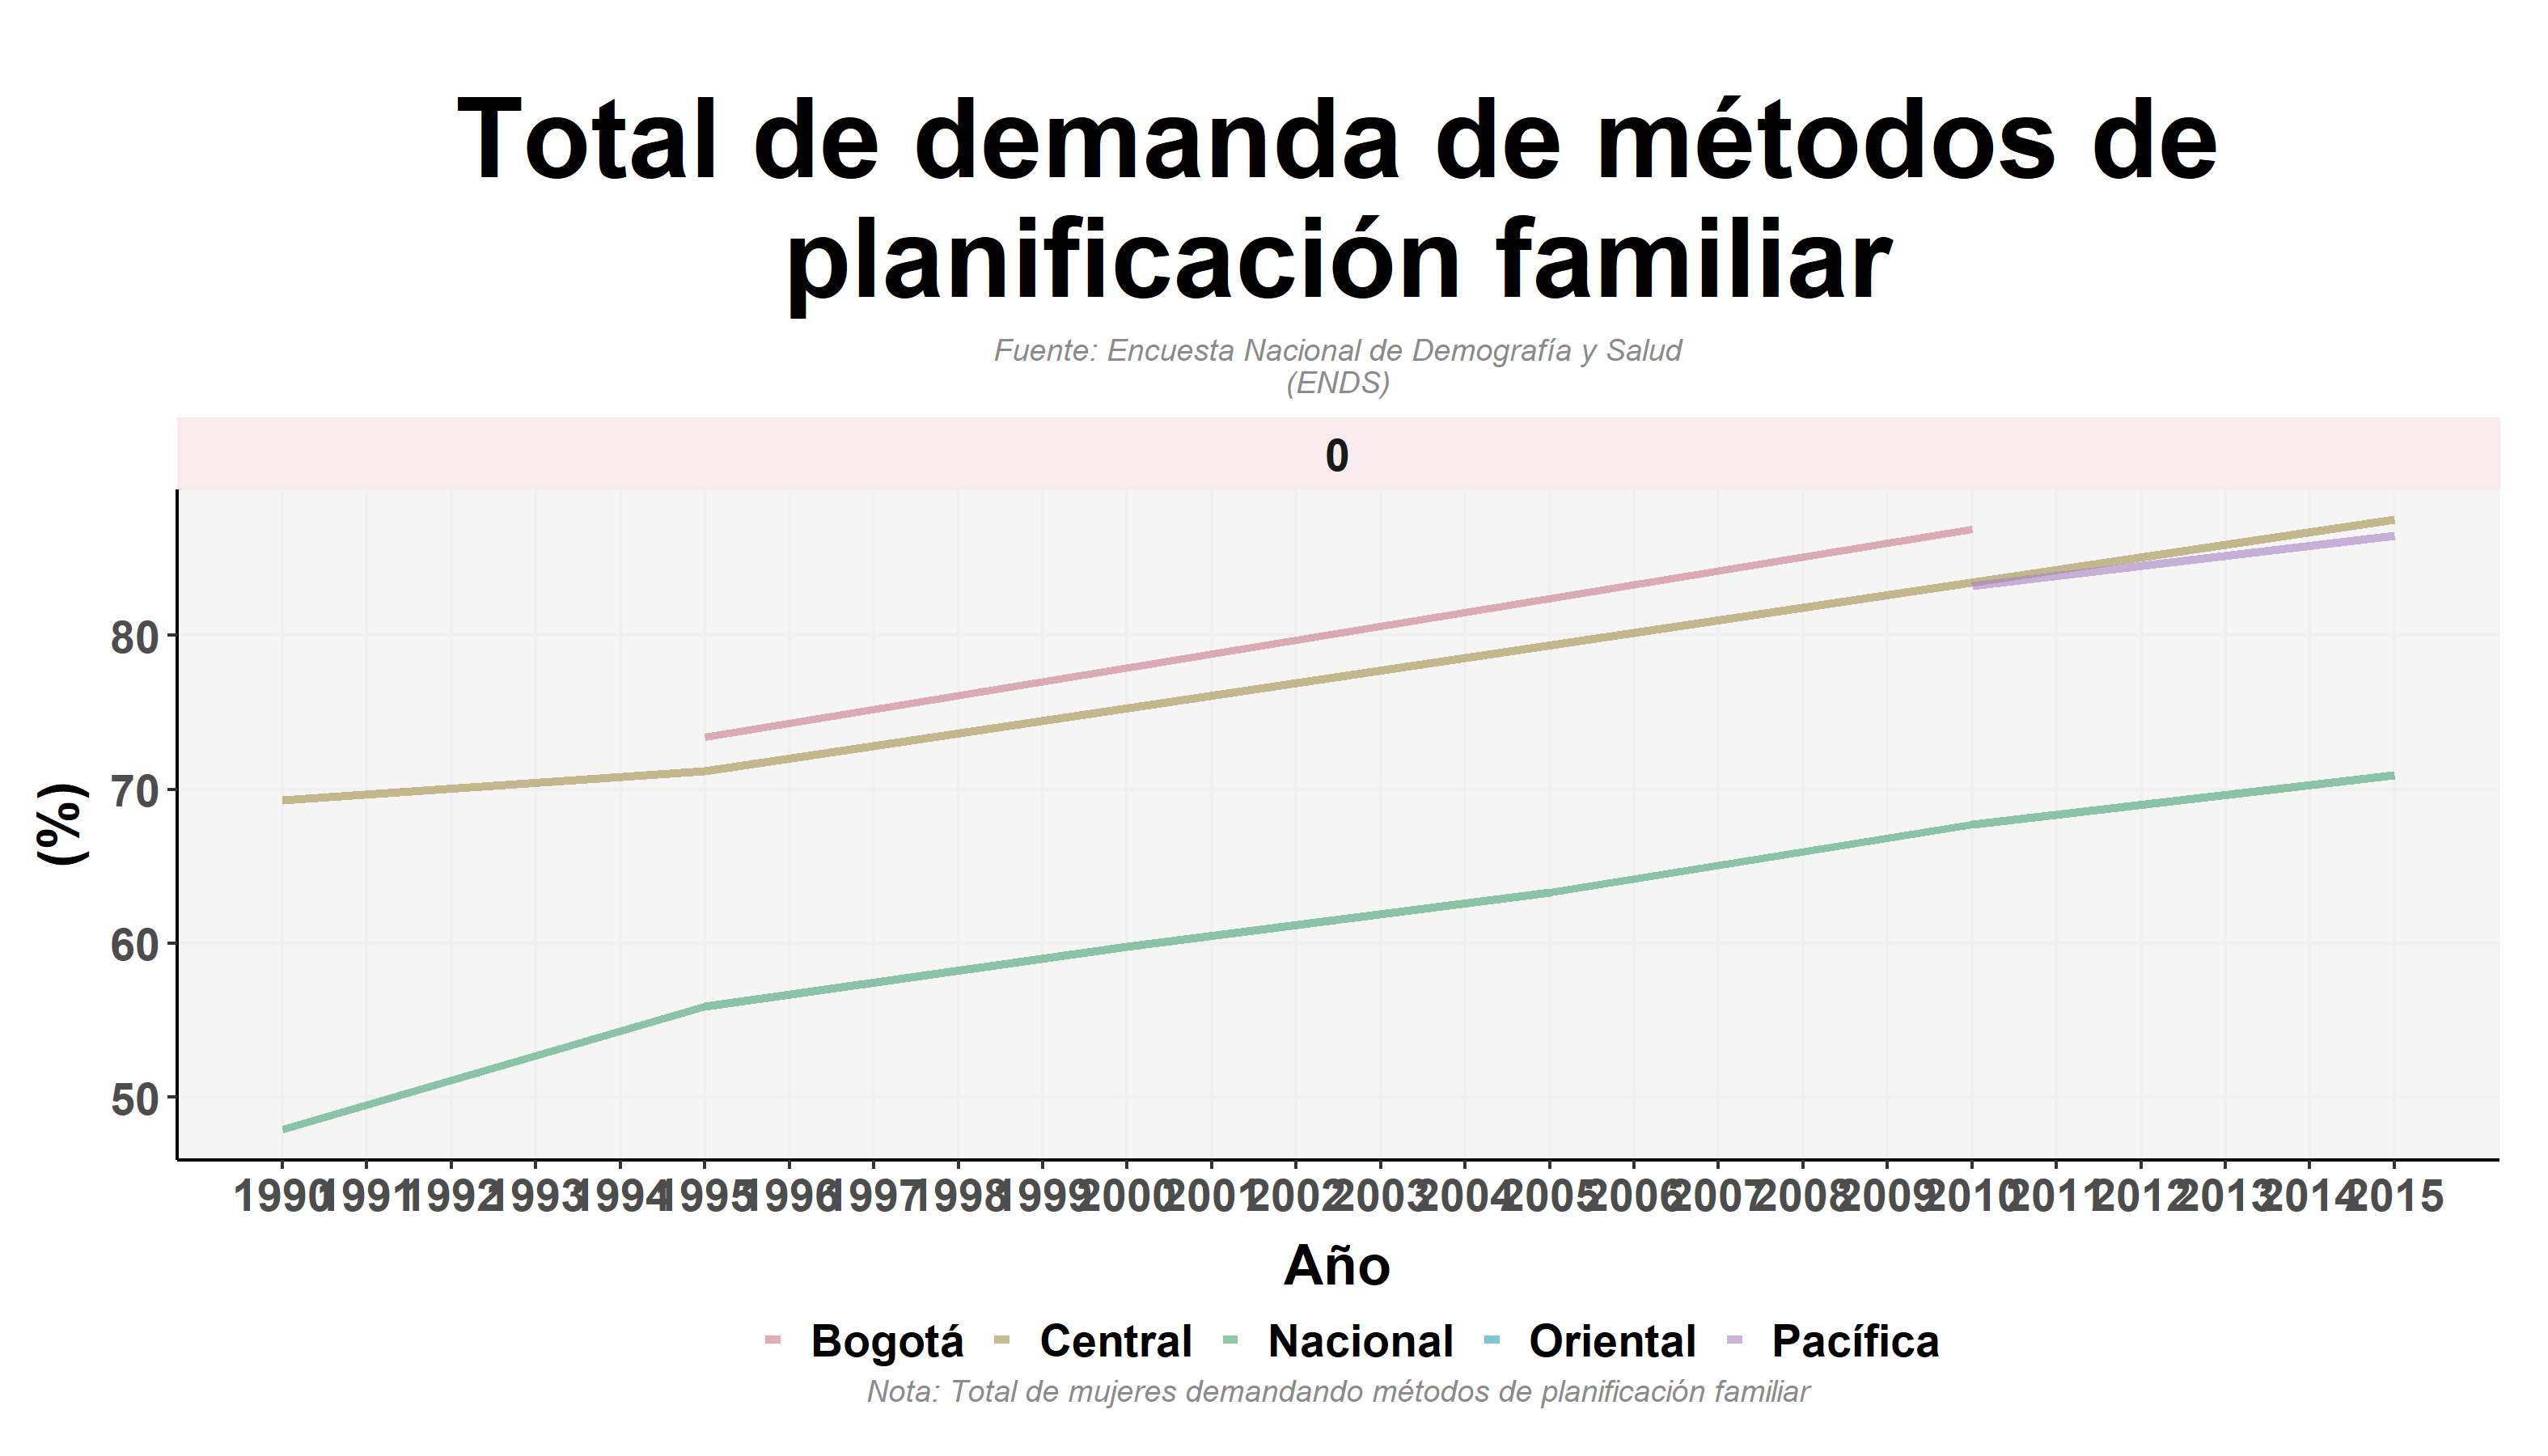
\includegraphics[width=\textwidth,keepaspectratio]{img/var_243_trend.png}
        \end{center}
    \end{figure}
            \begin{itemize}
                    \item Mientras que los niveles de pobreza aumentaron a nivel nacional y en las cabeceras, en los centros poblados y rural disperso esta disminuyó.
                    \item Los niveles de pobreza en las cabeceras y en las zonas rurales pasaron de tener brechas del más del 10\% hasta el 2019 a estar a niveles similares en el 2020.
                    \item El porcentaje de pobres a nivel nacional y en cabeceras tiene niveles superiores a los del 2012.
                    \end{itemize}

%%%% Include figures
    \begin{figure}[H]
        \caption{Población por clase social - Vulnerables (2012 VS 2020) por ciudad \label{map_result_2} }
        \begin{center}
        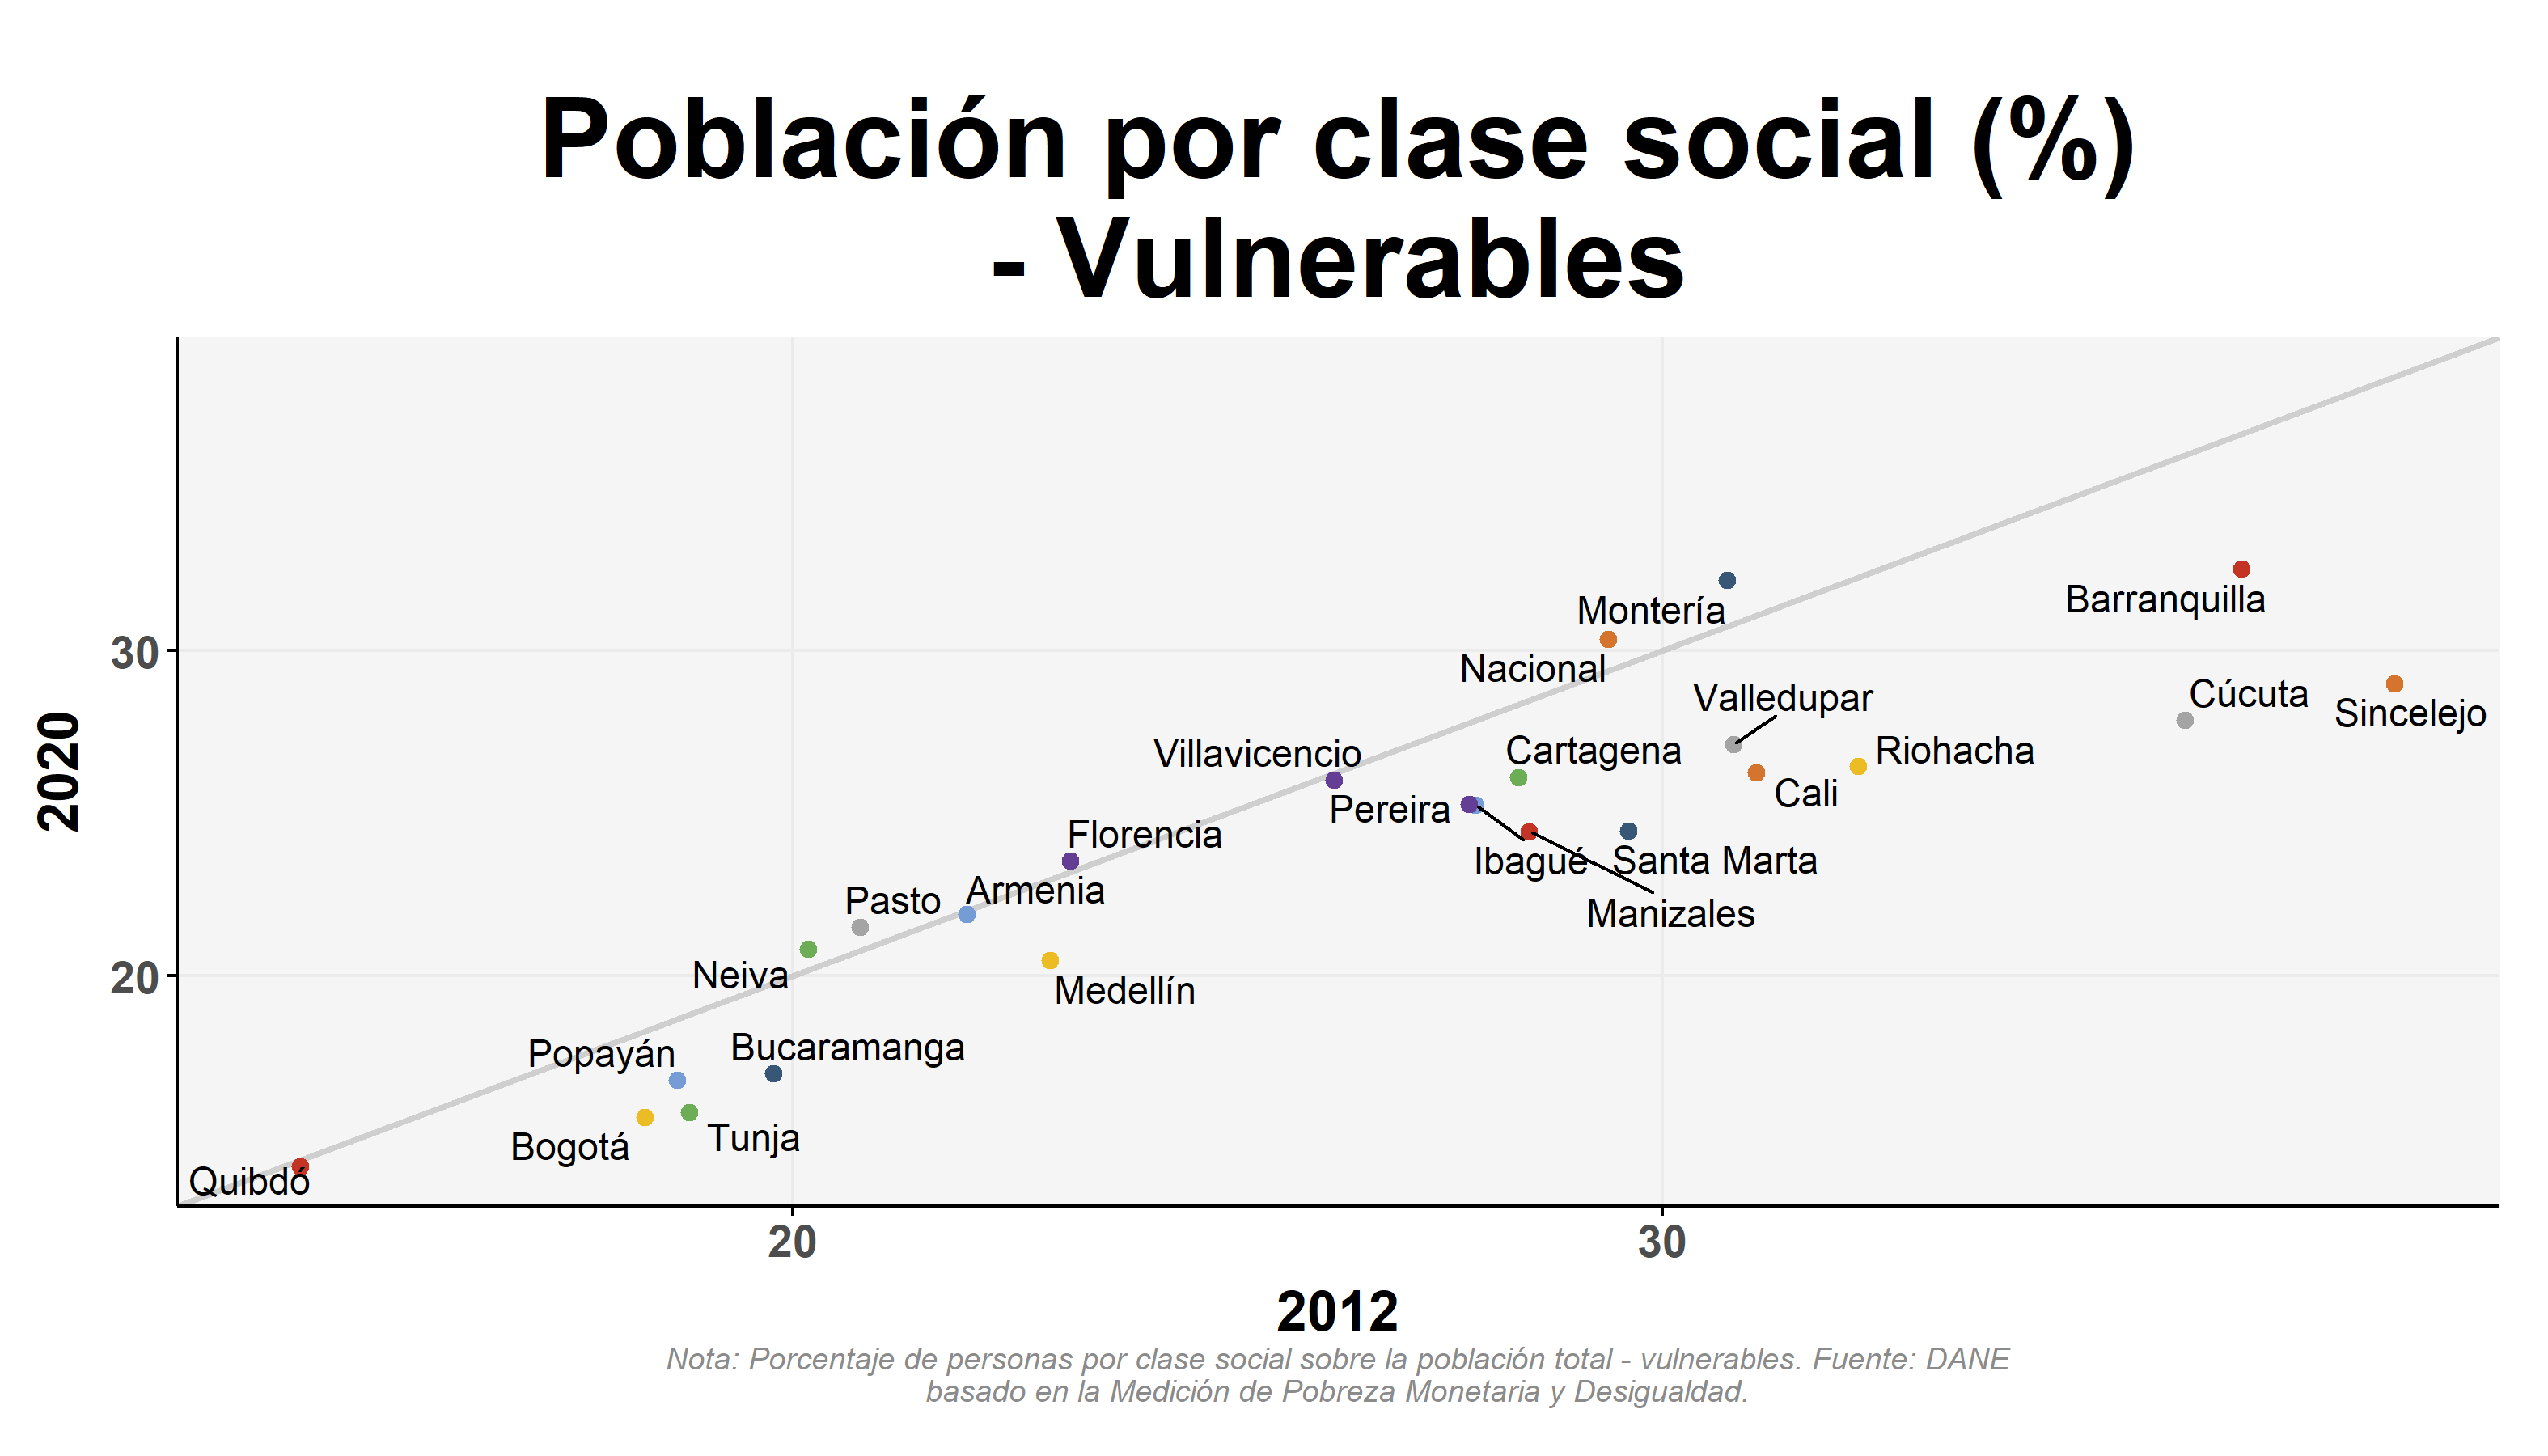
\includegraphics[width=\textwidth,keepaspectratio]{img/var_244_scatter_time.png}
        \end{center}
    \end{figure}
            \begin{itemize}
                    \item El porcentaje de vulnerables ha disminuido entre 2012 y 2020 en gran parte de las ciudades principales.
                    \item Ciudades como Villavicencio, Florencia, Quibdó y Armenia se mantienen a los mismos niveles de 2012.
                    \item A nivel nacional el porcentaje de vulnerables aumentó con respecto al 2012 levemente para el 2020.
                    \item Quibdó para ambos años de referencia es el de menor porcentaje de vulnerables.
                    \item La diferencia entre la ciudad con mayor nivel de población vulnerable (Barranquilla) y la de menor nivel de población (Quibdó) es de alrededor de 15\%.
                    \end{itemize}

%%%% Include figures
    \begin{figure}[H]
        \caption{Población por clase social - Vulnerables a nivel nacional \label{map_result_2} }
        \begin{center}
        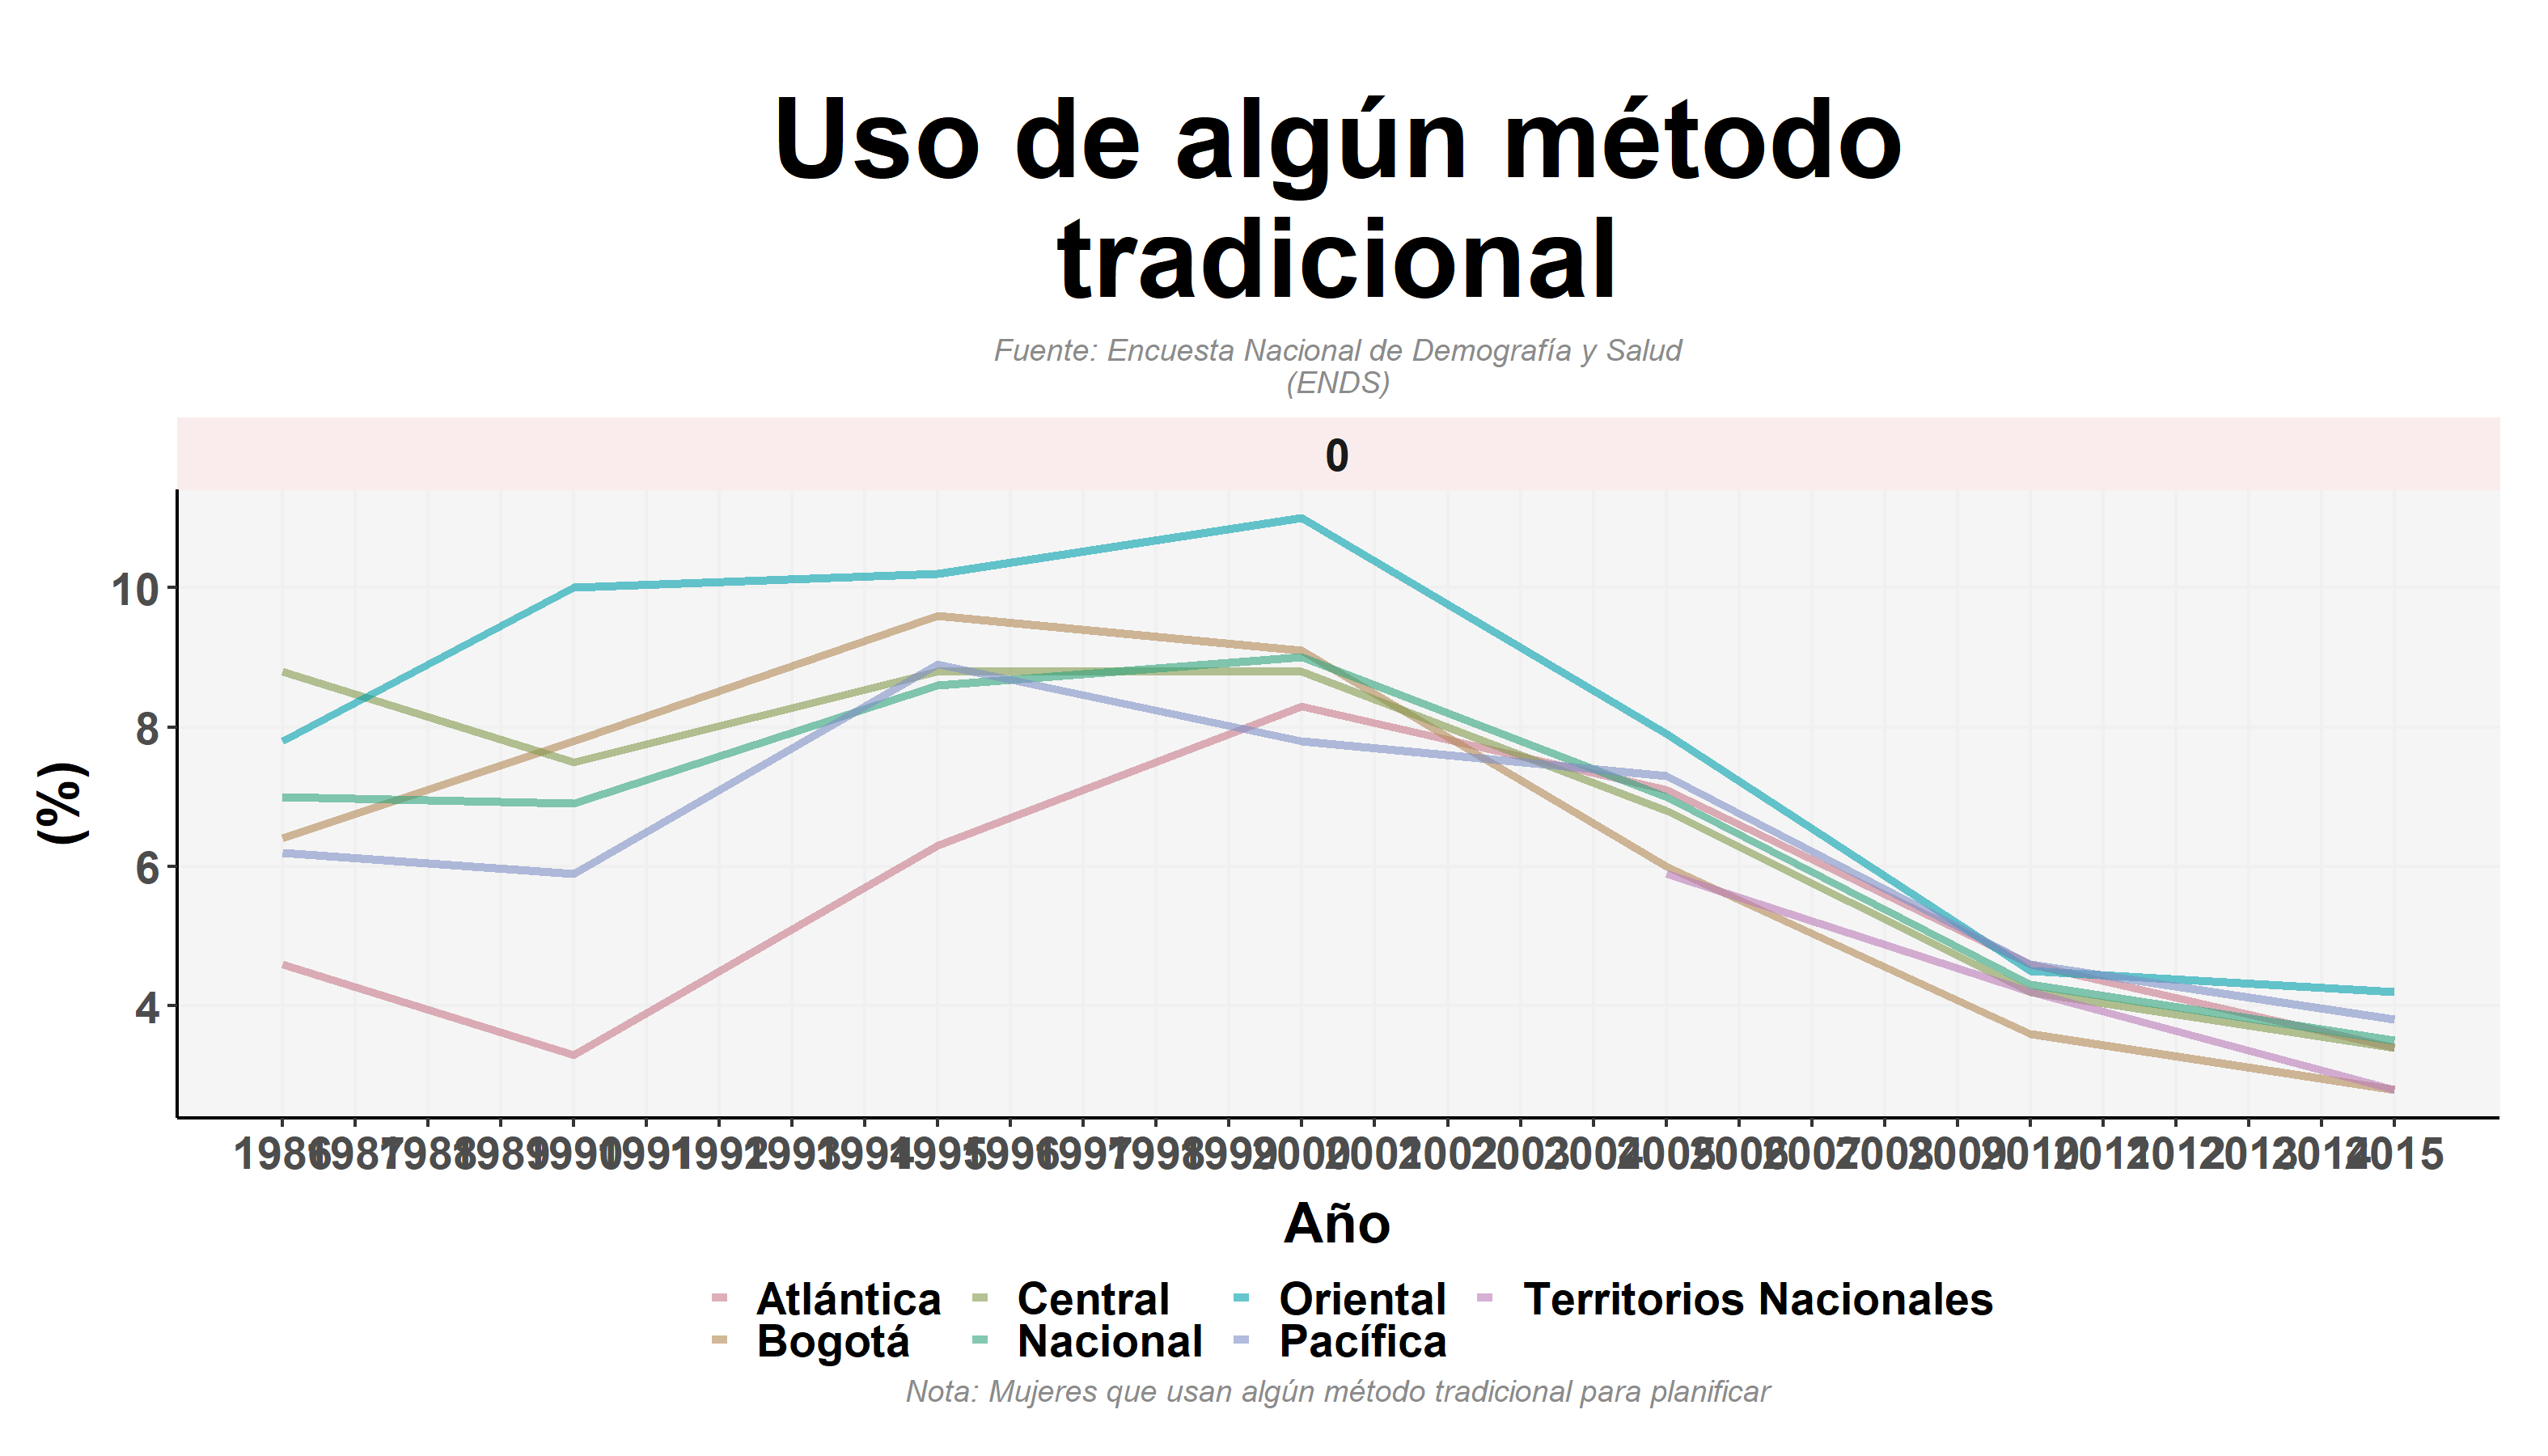
\includegraphics[width=\textwidth,keepaspectratio]{img/var_245_trend.png}
        \end{center}
    \end{figure}
            \begin{itemize}
                    \item El porcentaje de vulnerables estaba aumentando hasta 2018, a partir de ahí empieza a decaer intensificándose en el 2020.
                    \item Para 2020 el porcentaje de vulnerables tiene un retroceso cercano a los niveles del 2013.
                    \item Para el 2016 el porcentaje de vulnerables disminuyó con respecto al año anterior, pero se recuperó y aumentó en el año siguiente.
                    \end{itemize}

%%%% Include figures
    \begin{figure}[H]
        \caption{Población por clase social - Vulnerables por zonas \label{map_result_2} }
        \begin{center}
        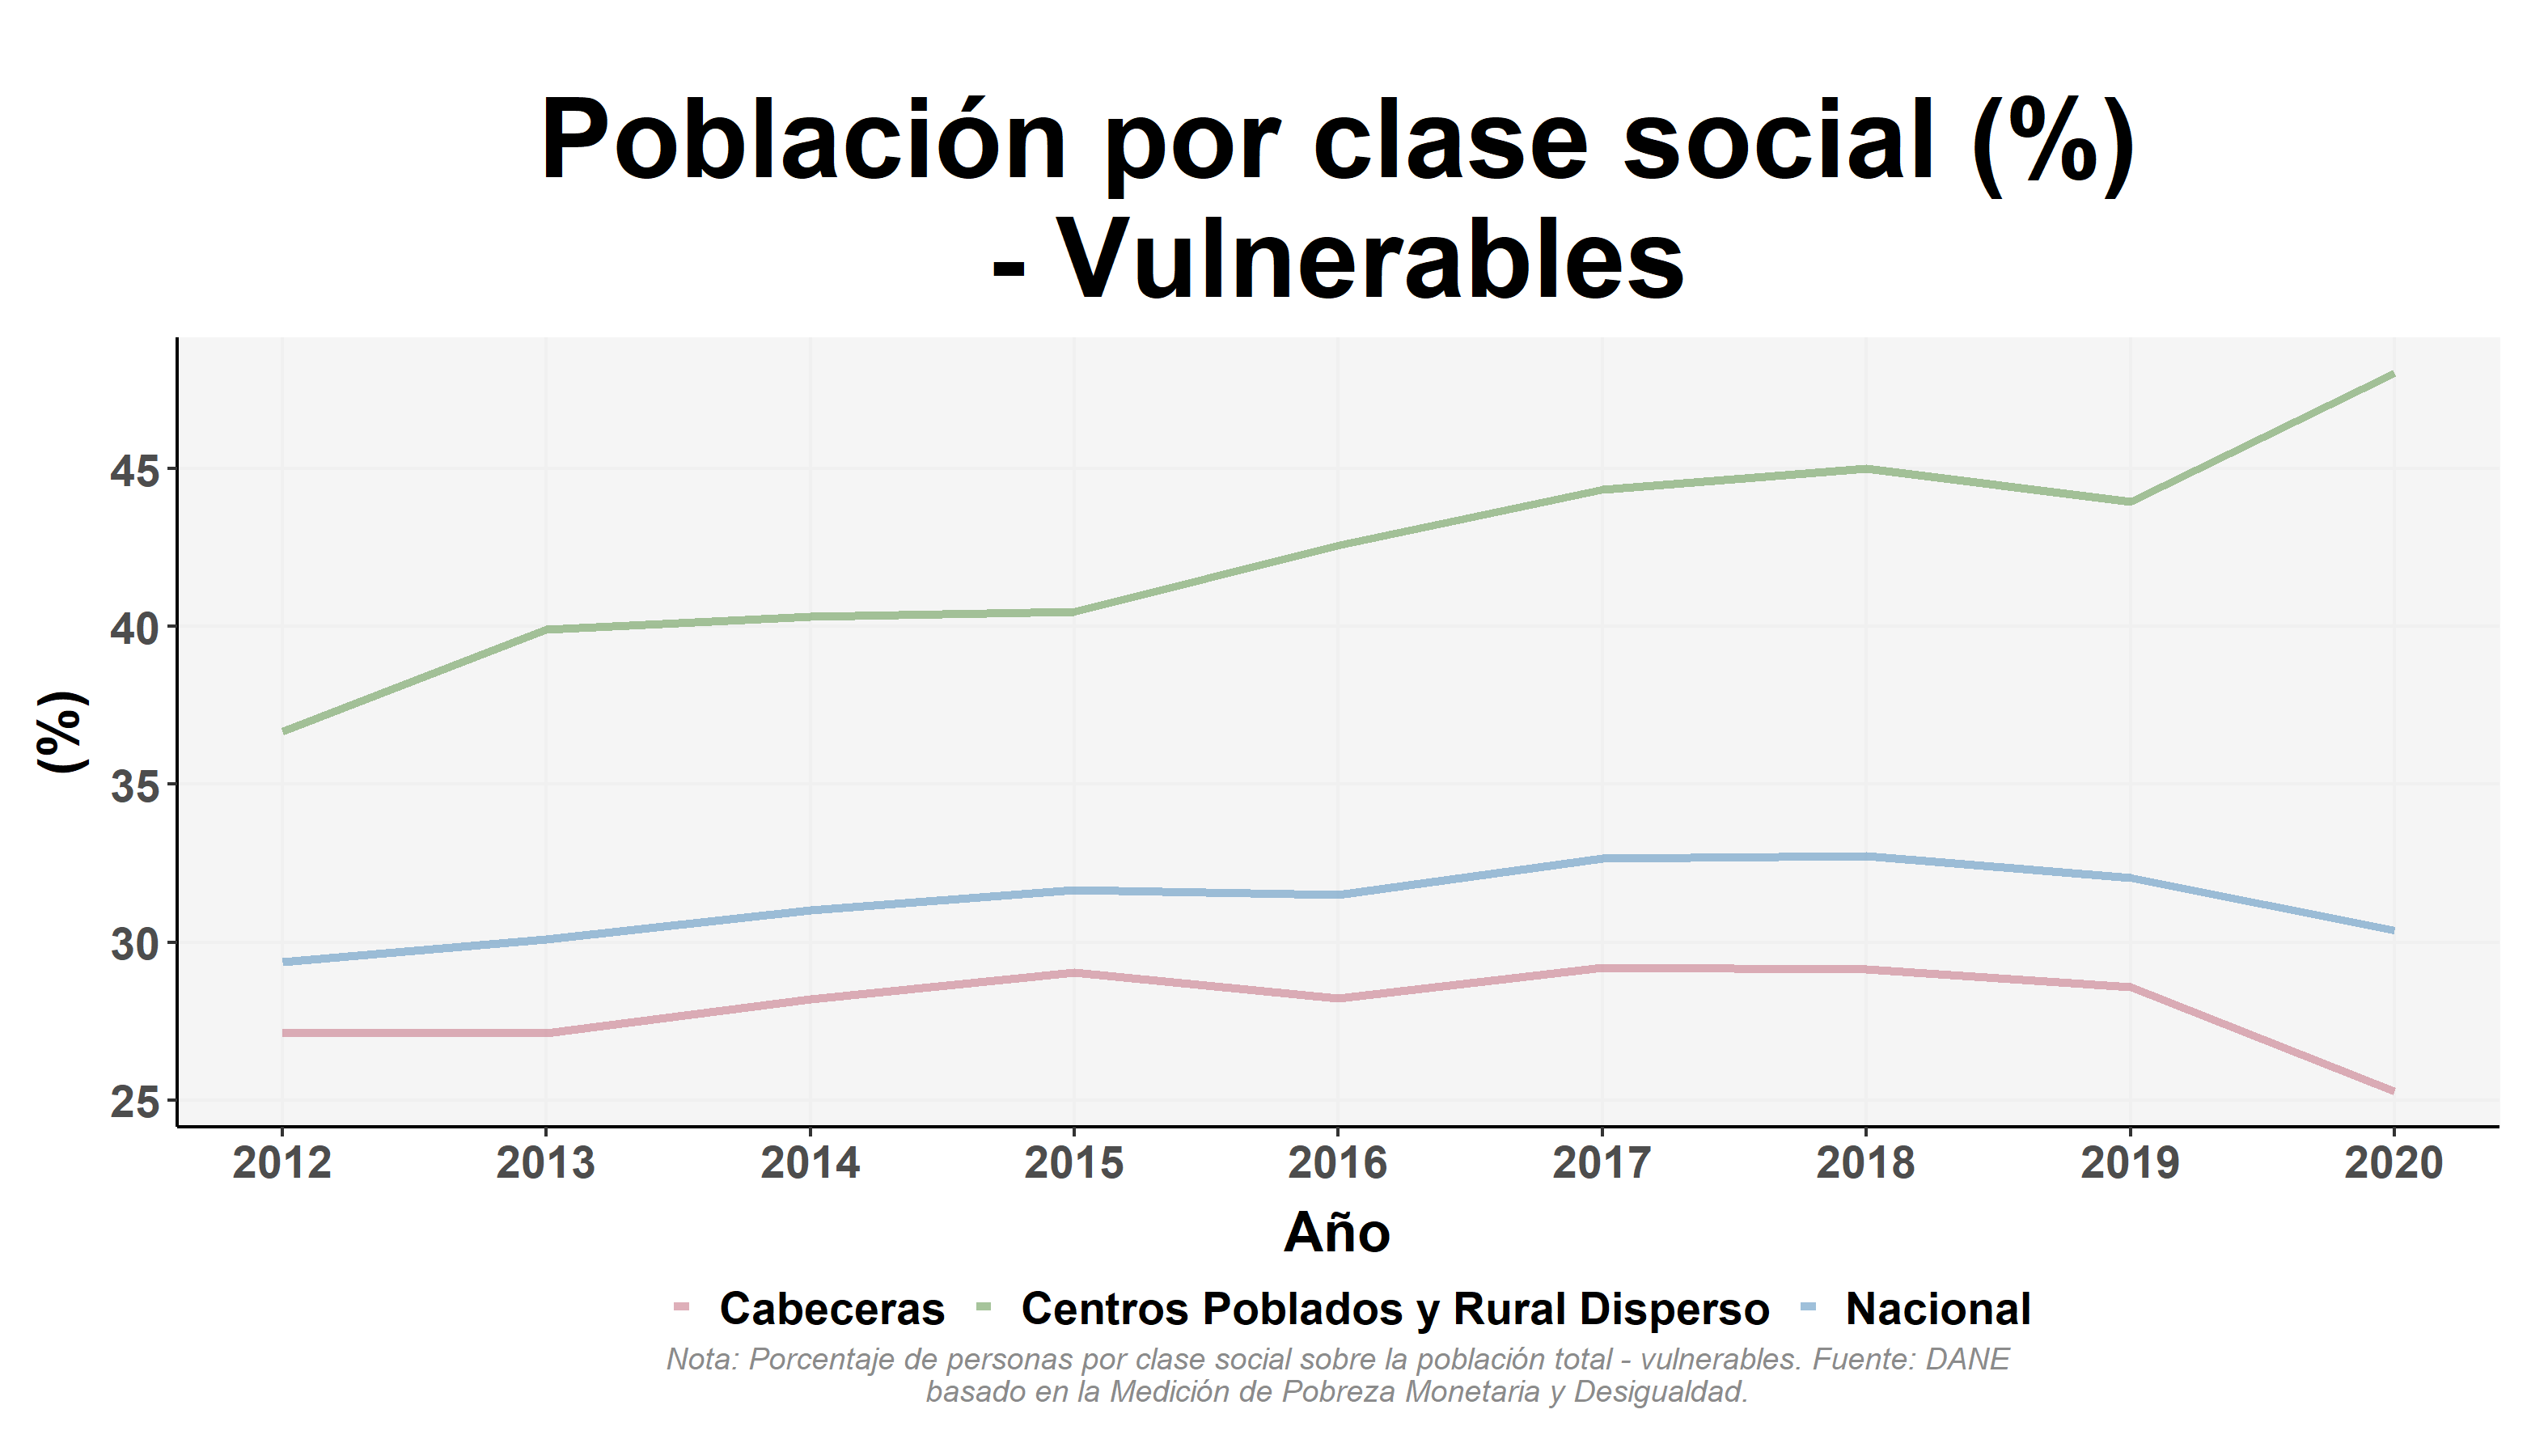
\includegraphics[width=\textwidth,keepaspectratio]{img/var_246_trend.png}
        \end{center}
    \end{figure}
            \begin{itemize}
                    \item En los centros poblados y rural disperso ha venido aumentando y fue el único que lo hizo para el 2020.
                    \item A nivel nacional y las cabeceras el porcentaje de vulnerables disminuyó desde el 2018 y se intensificó para el 2020.
                    \item Las cabeceras tienen niveles de vulnerables menores a los reportados en 2012, mientras que a nivel nacional son cercanos pero aun superiores.
                    \end{itemize}

%%%% Include figures
    \begin{figure}[H]
        \caption{Población por clase social - Clase media (2012 VS 2020) por ciudades \label{map_result_2} }
        \begin{center}
        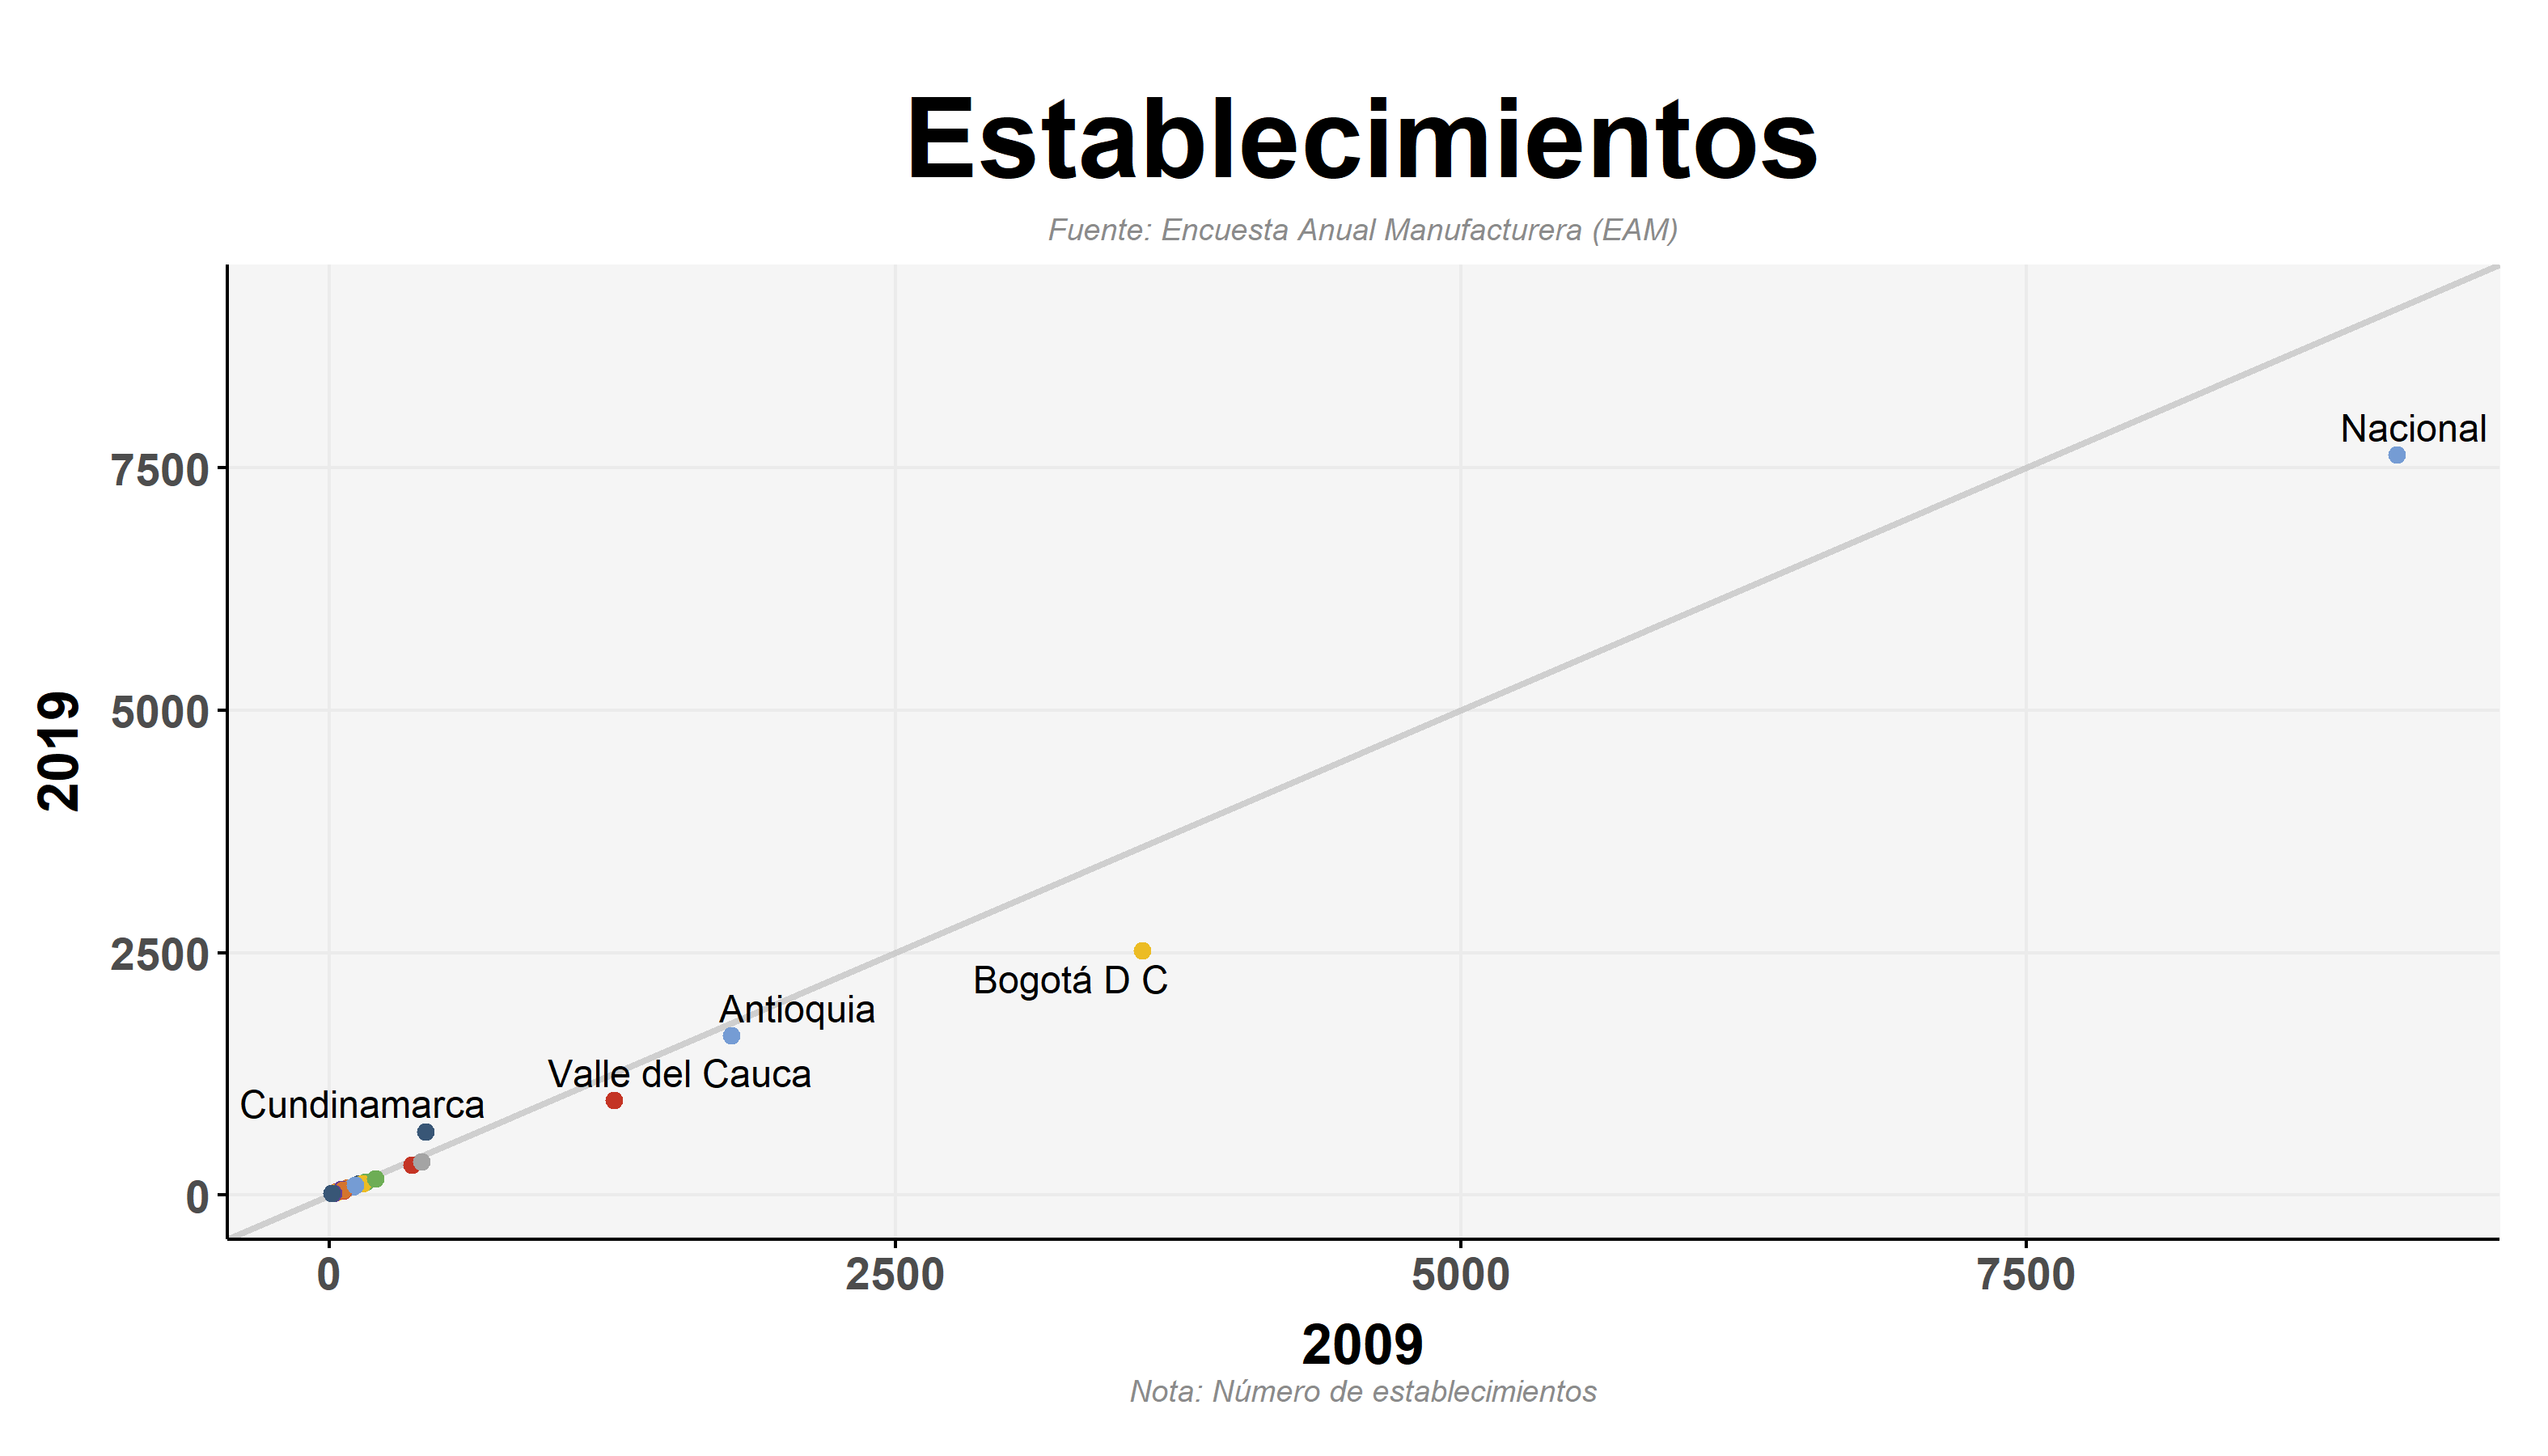
\includegraphics[width=\textwidth,keepaspectratio]{img/var_247_scatter_time.png}
        \end{center}
    \end{figure}
            \begin{itemize}
                    \item Pasto, Popayán y Quibdó mejoraron para 2020 el porcentaje de clase media con respecto a los registrados en 2012.
                    \item Florencia, Armenia y Cali registraron un porcentaje de clase social en 2020 iguales a los de 2012.
                    \item Las demás ciudades principales registraron niveles menores de población en clase media en 2020 comparado con los de 2012.
                    \item Para 2020 la diferencia entre las ciudades extremo es poco más del 25\% (Medellín - Riohacha).
                    \end{itemize}

%%%% Include figures
    \begin{figure}[H]
        \caption{Población por clase social - Clase media a nivel nacional \label{map_result_2} }
        \begin{center}
        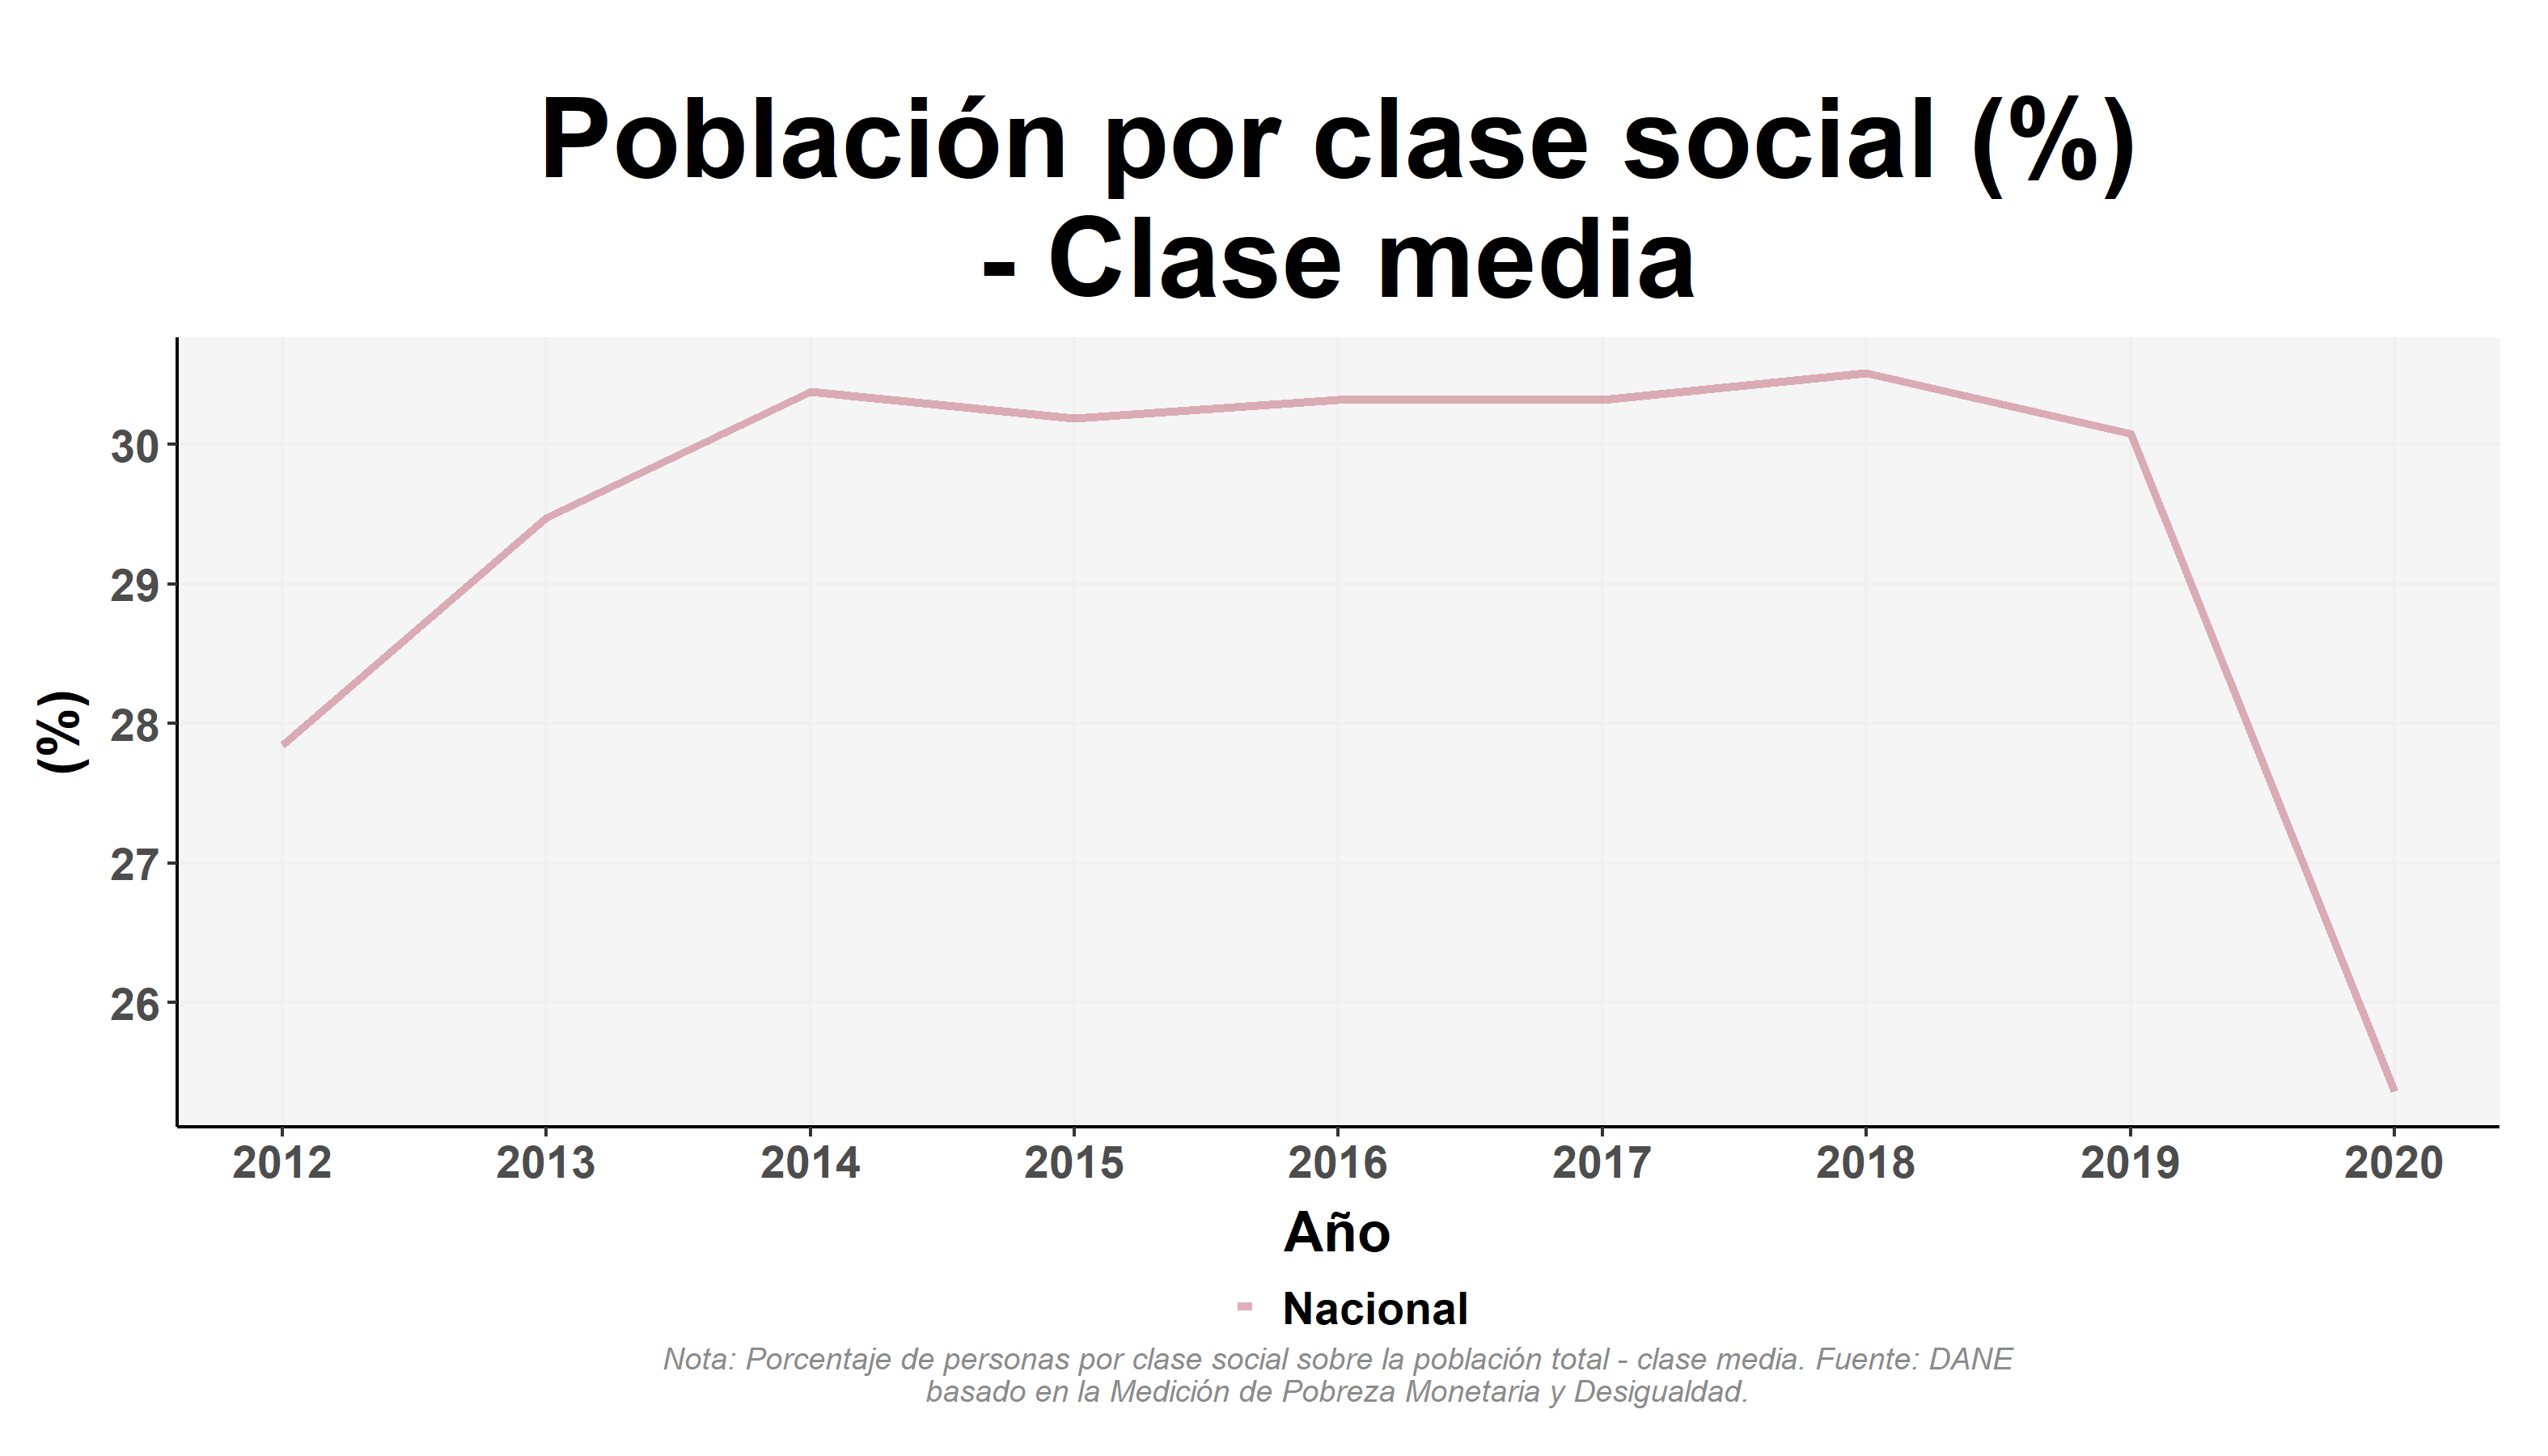
\includegraphics[width=\textwidth,keepaspectratio]{img/var_248_trend.png}
        \end{center}
    \end{figure}
            \begin{itemize}
                    \item El porcentaje de clase media a nivel nacional estuvo estancado después del 2014 hasta el 2018, donde empezó a disminuir.
                    \item A partir del 2018 empieza a decaer, lo cual se intensifica en el 2020.
                    \item El nivel de porcentaje de clase media para el 2020 está por debajo de los registrados en el 2012.
                    \item Desde el 2012 hasta el 2014 el porcentaje de personas de clase media estaba en aumento.
                    \end{itemize}

%%%% Include figures
    \begin{figure}[H]
        \caption{Población por clase social - Clase media por zonas \label{map_result_2} }
        \begin{center}
        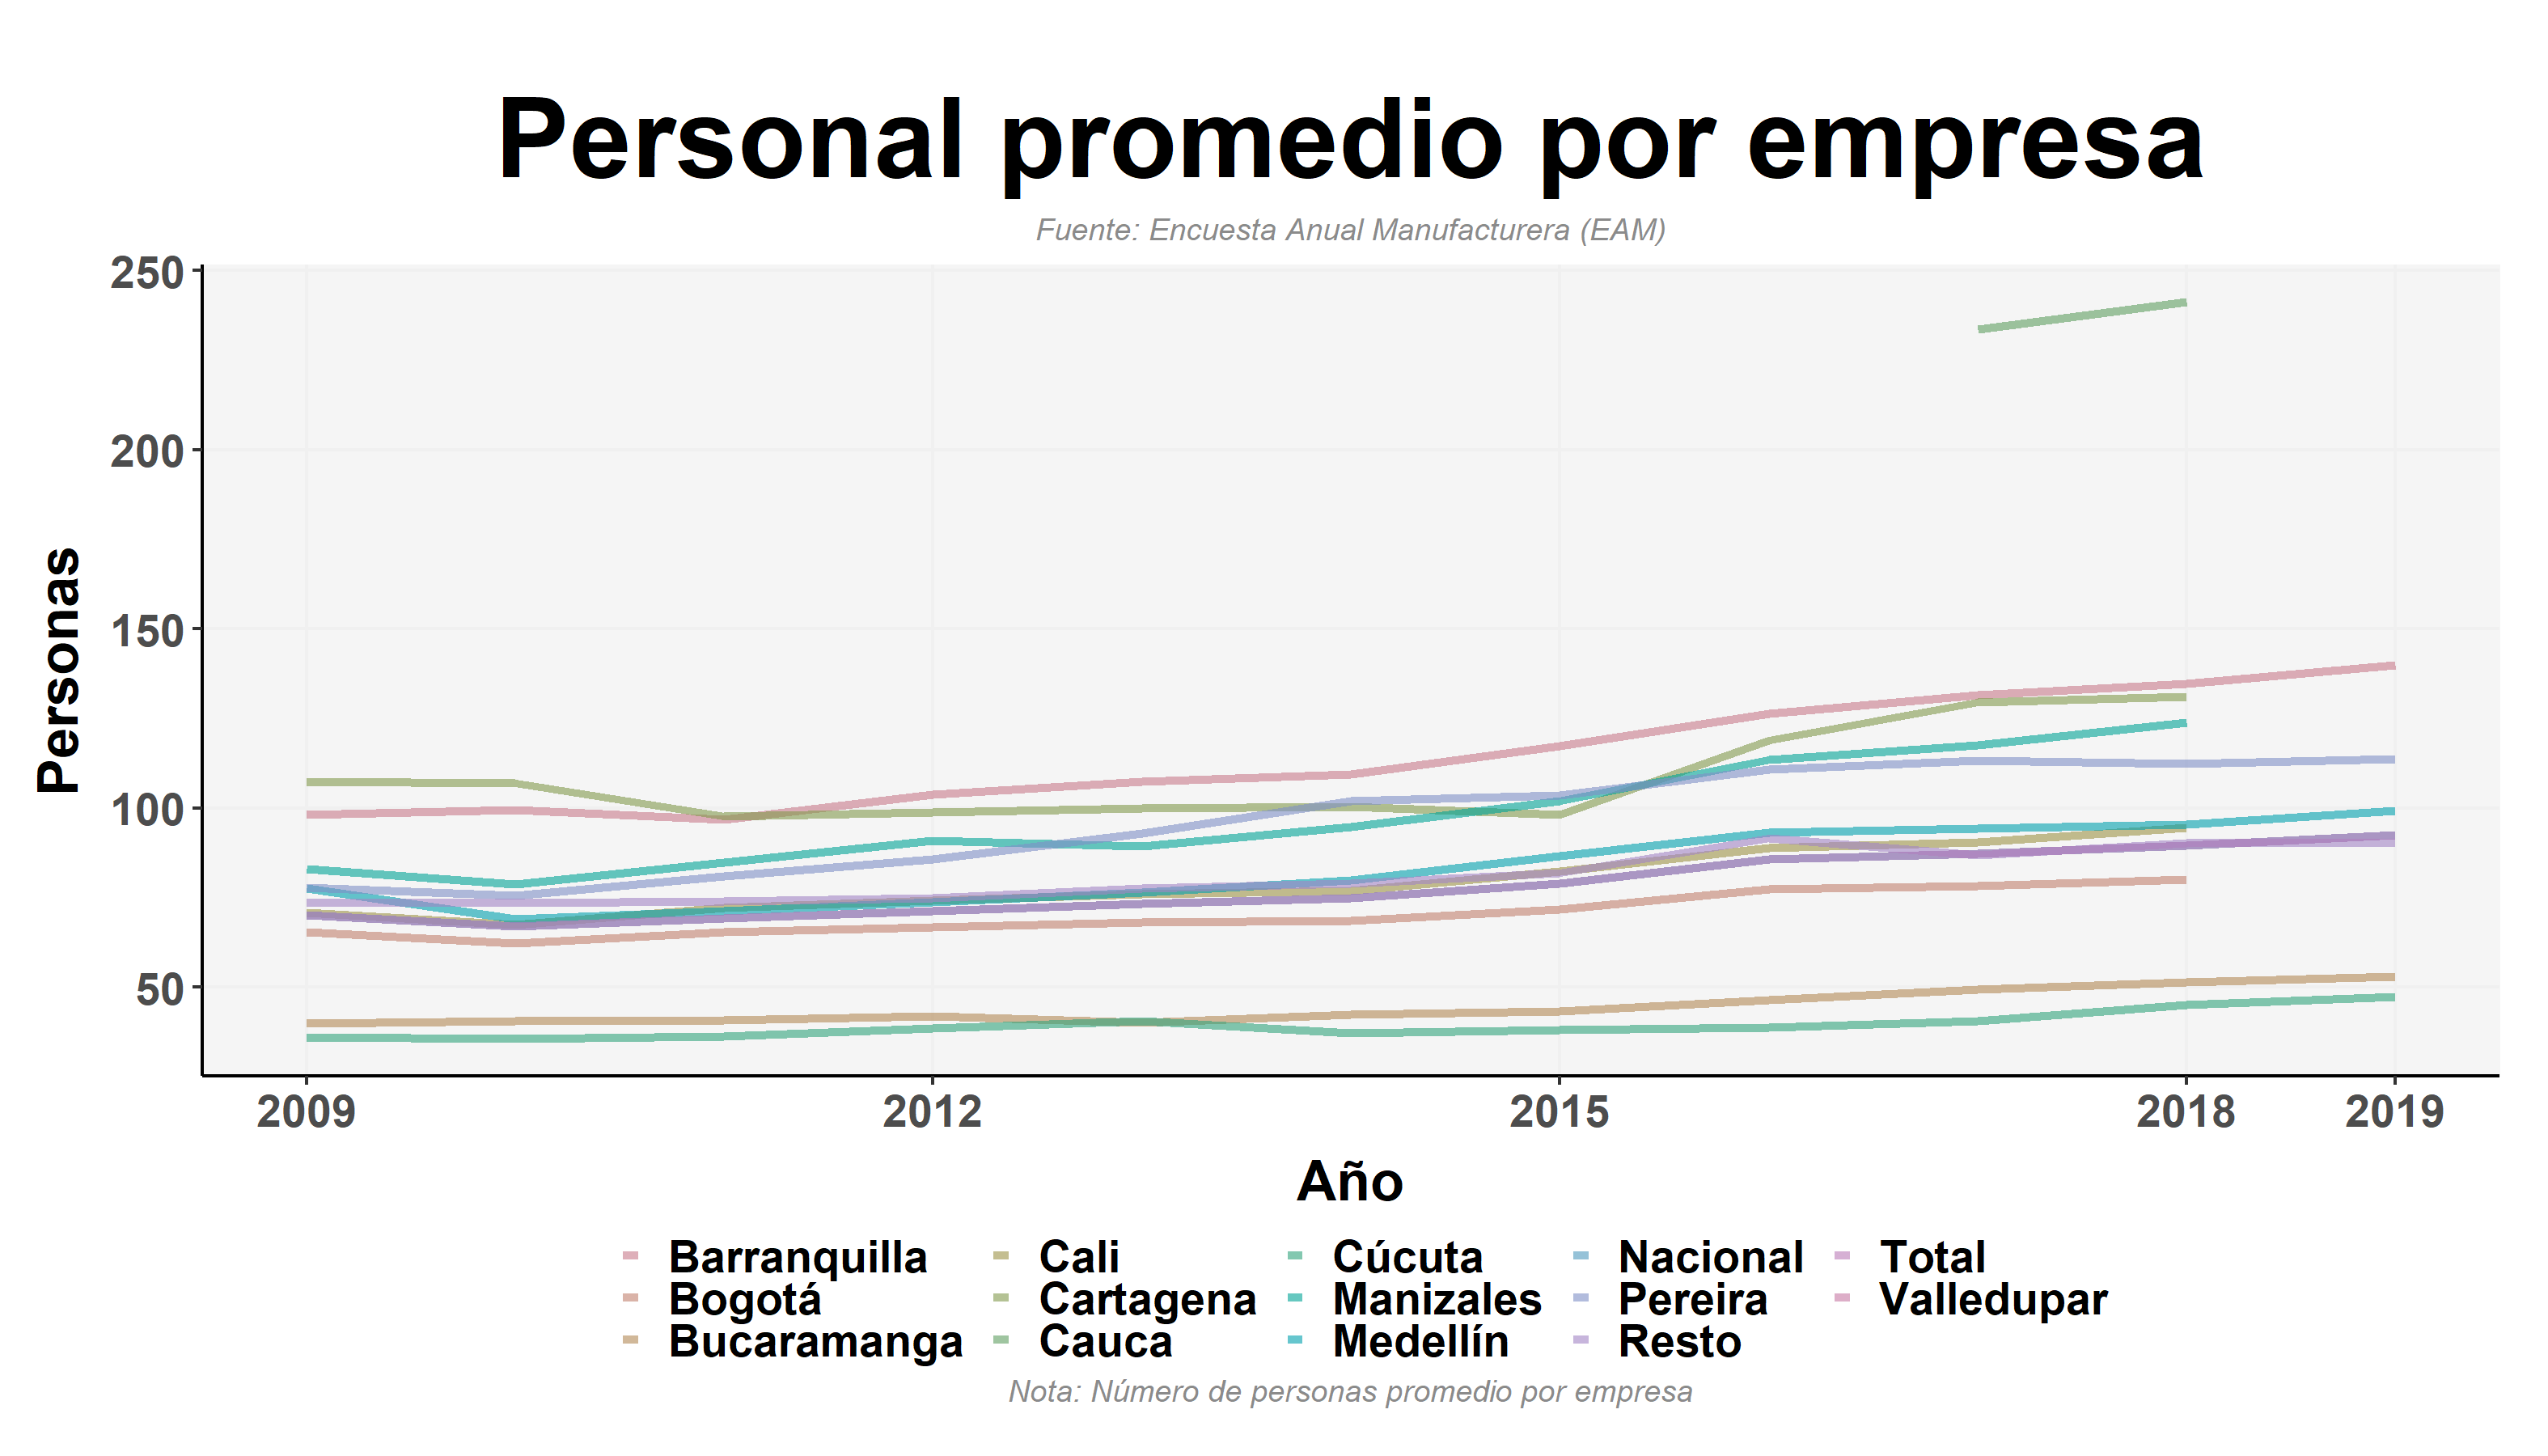
\includegraphics[width=\textwidth,keepaspectratio]{img/var_249_trend.png}
        \end{center}
    \end{figure}
            \begin{itemize}
                    \item Para los centros poblados y rural disperso los niveles de personas de clase media han tenido un leve aumento hasta el 2017 donde inicio a decaer pero se recuperó para el 2020.
                    \item A nivel nacional y cabeceras los niveles de clase media han estado constantes hasta el 2019, en el 2020 presenta una caída abrupta.
                    \item Para 2020 los niveles registrados de clase media a nivel nacional y cabeceras son menores a los registrados en el 2012.
                    \end{itemize}

%%%% Include figures
    \begin{figure}[H]
        \caption{Población por clase social - Clase alta (2012 VS 2020) por ciudad \label{map_result_2} }
        \begin{center}
        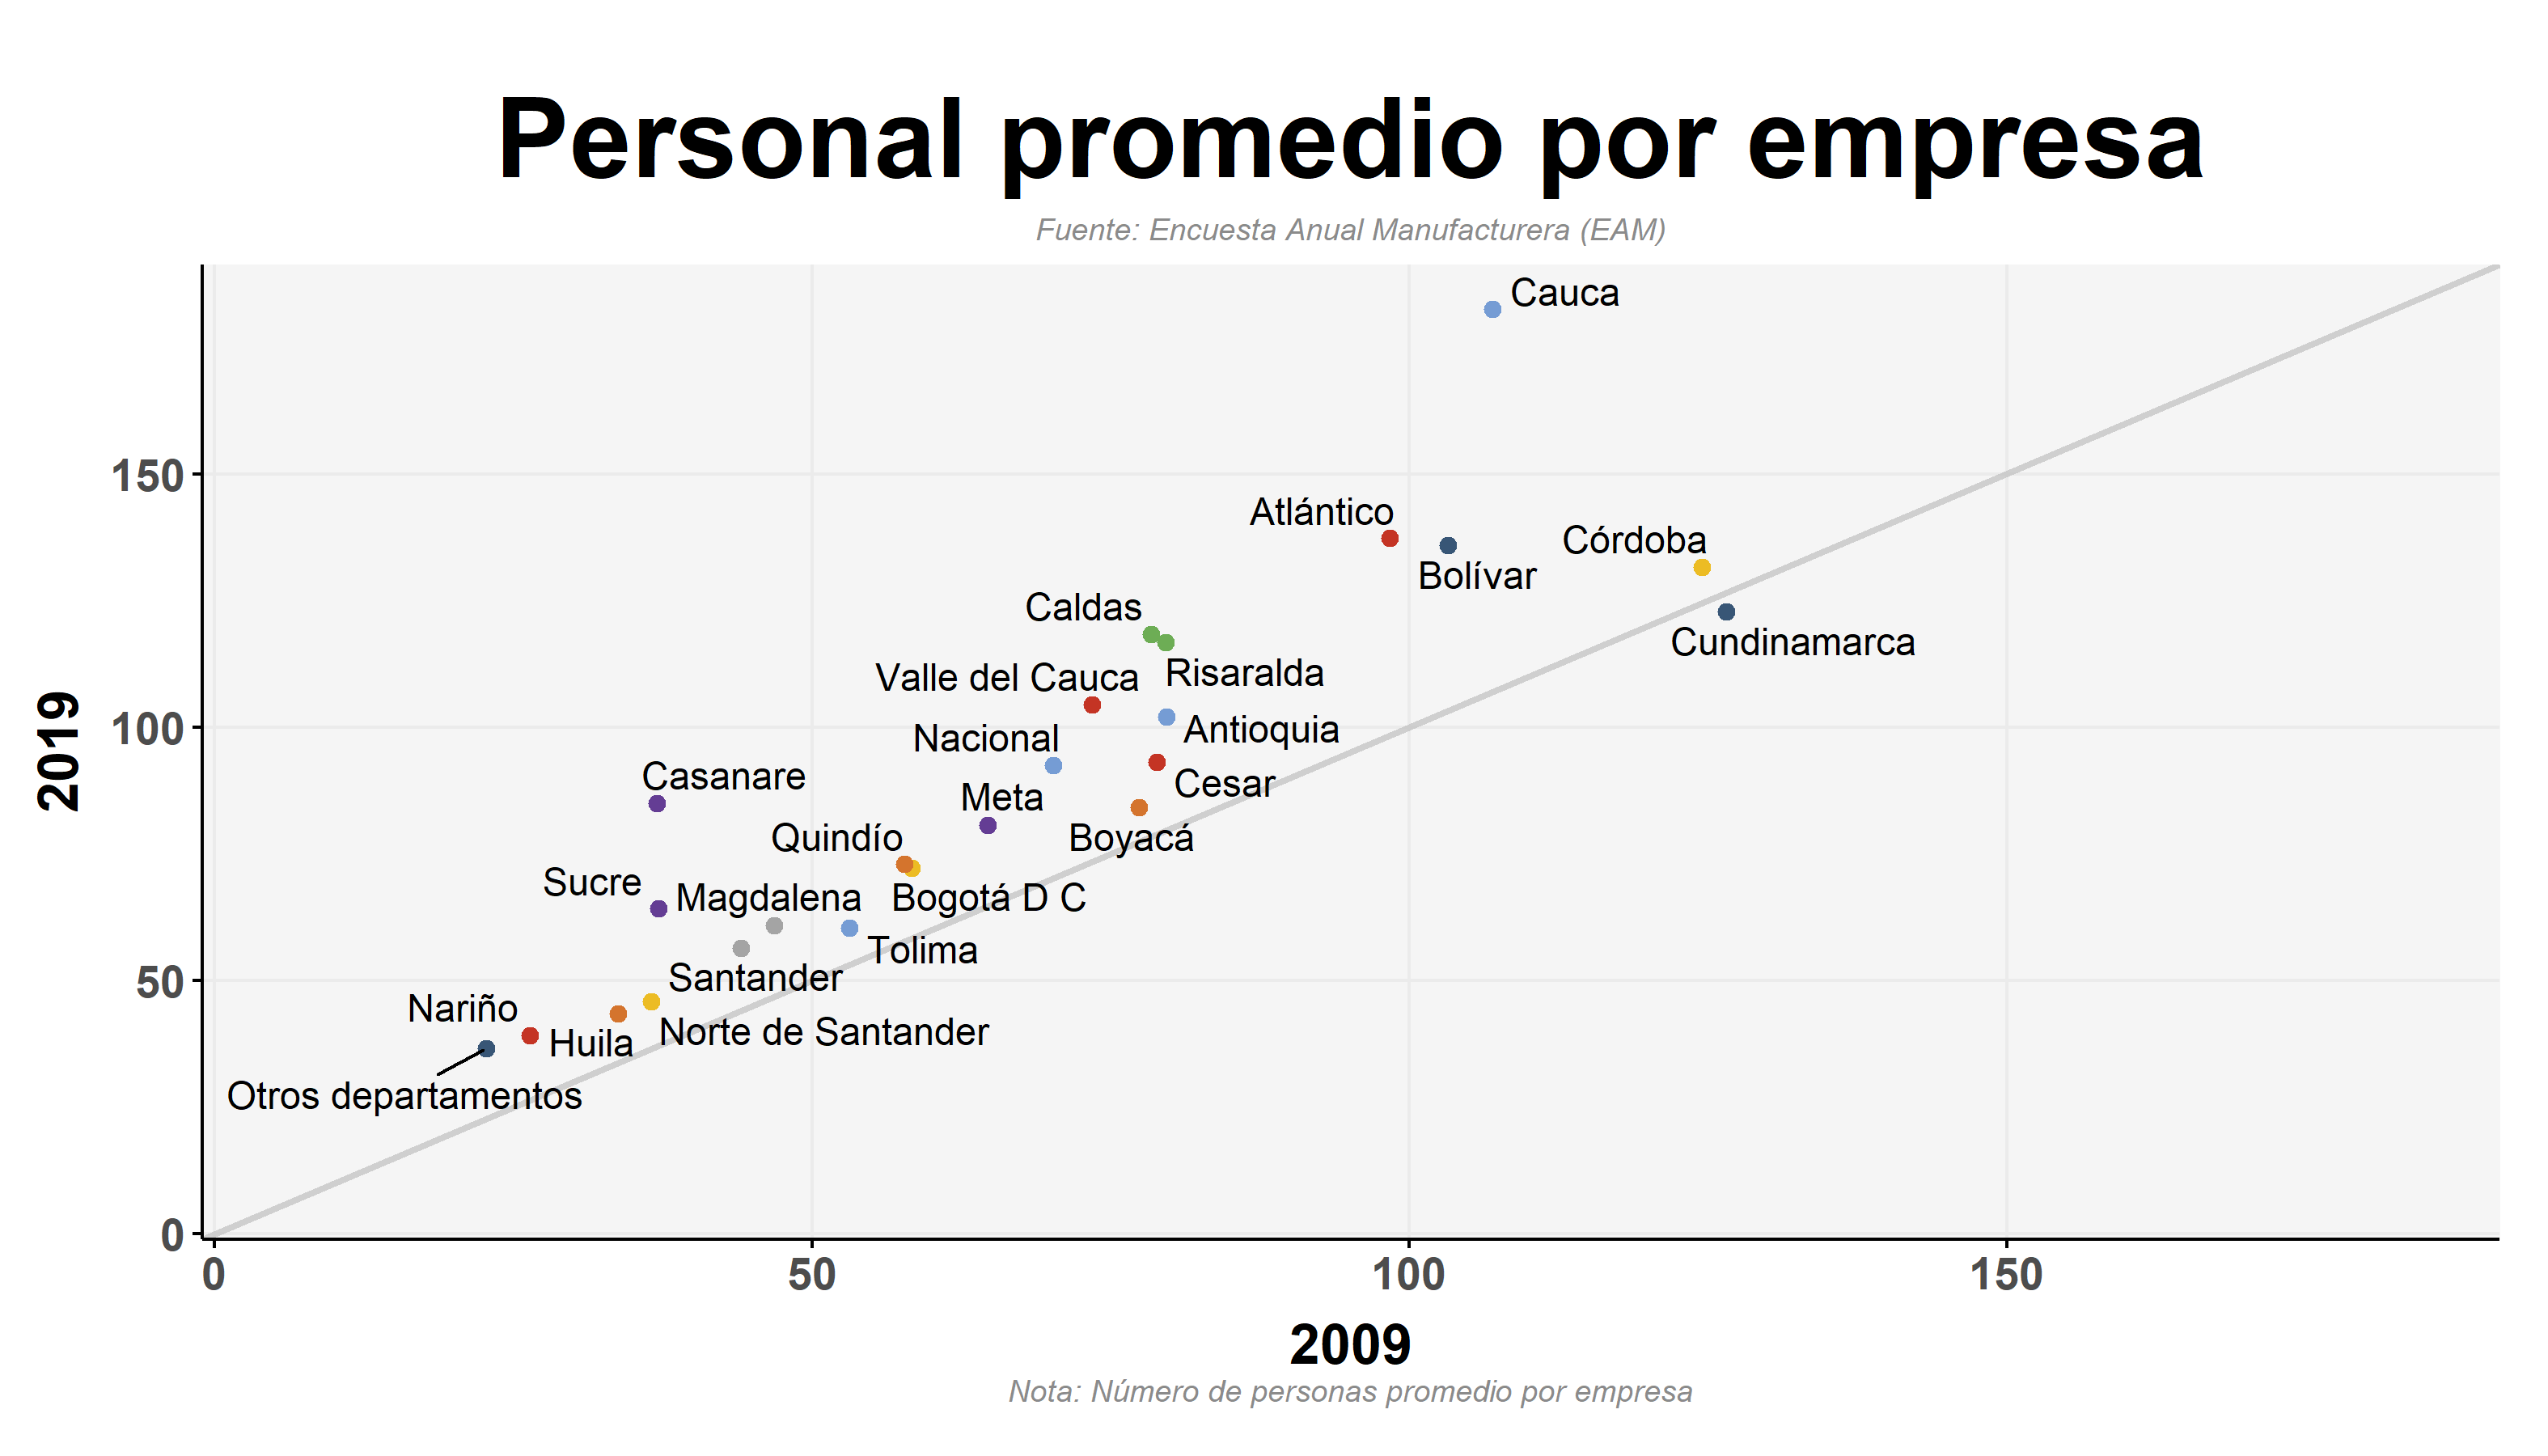
\includegraphics[width=\textwidth,keepaspectratio]{img/var_250_scatter_time.png}
        \end{center}
    \end{figure}
            \begin{itemize}
                    \item Pasto es la única ciudad que presenta mejores niveles de clase alta en el 2020, comparado con los de 2012.
                    \item Cúcuta y Barranquilla presentan niveles de clase alta similares entre 2012 y 2020.
                    \item Medellín y Bogotá son las ciudades con más alto nivel de población de clase alta estando alejadas de las otras ciudades.
                    \item Hay una diferencia de 4\% entre las ciudades extremo (Medellín - Riohacha).
                    \item Ninguna ciudad presenta una población de clase alta por encima del 5\%, gran parte de las ciudades está por debajo del 3\%.
                    \end{itemize}

%%%% Include figures
    \begin{figure}[H]
        \caption{Población por clase social - Clase alta a nivel nacional \label{map_result_2} }
        \begin{center}
        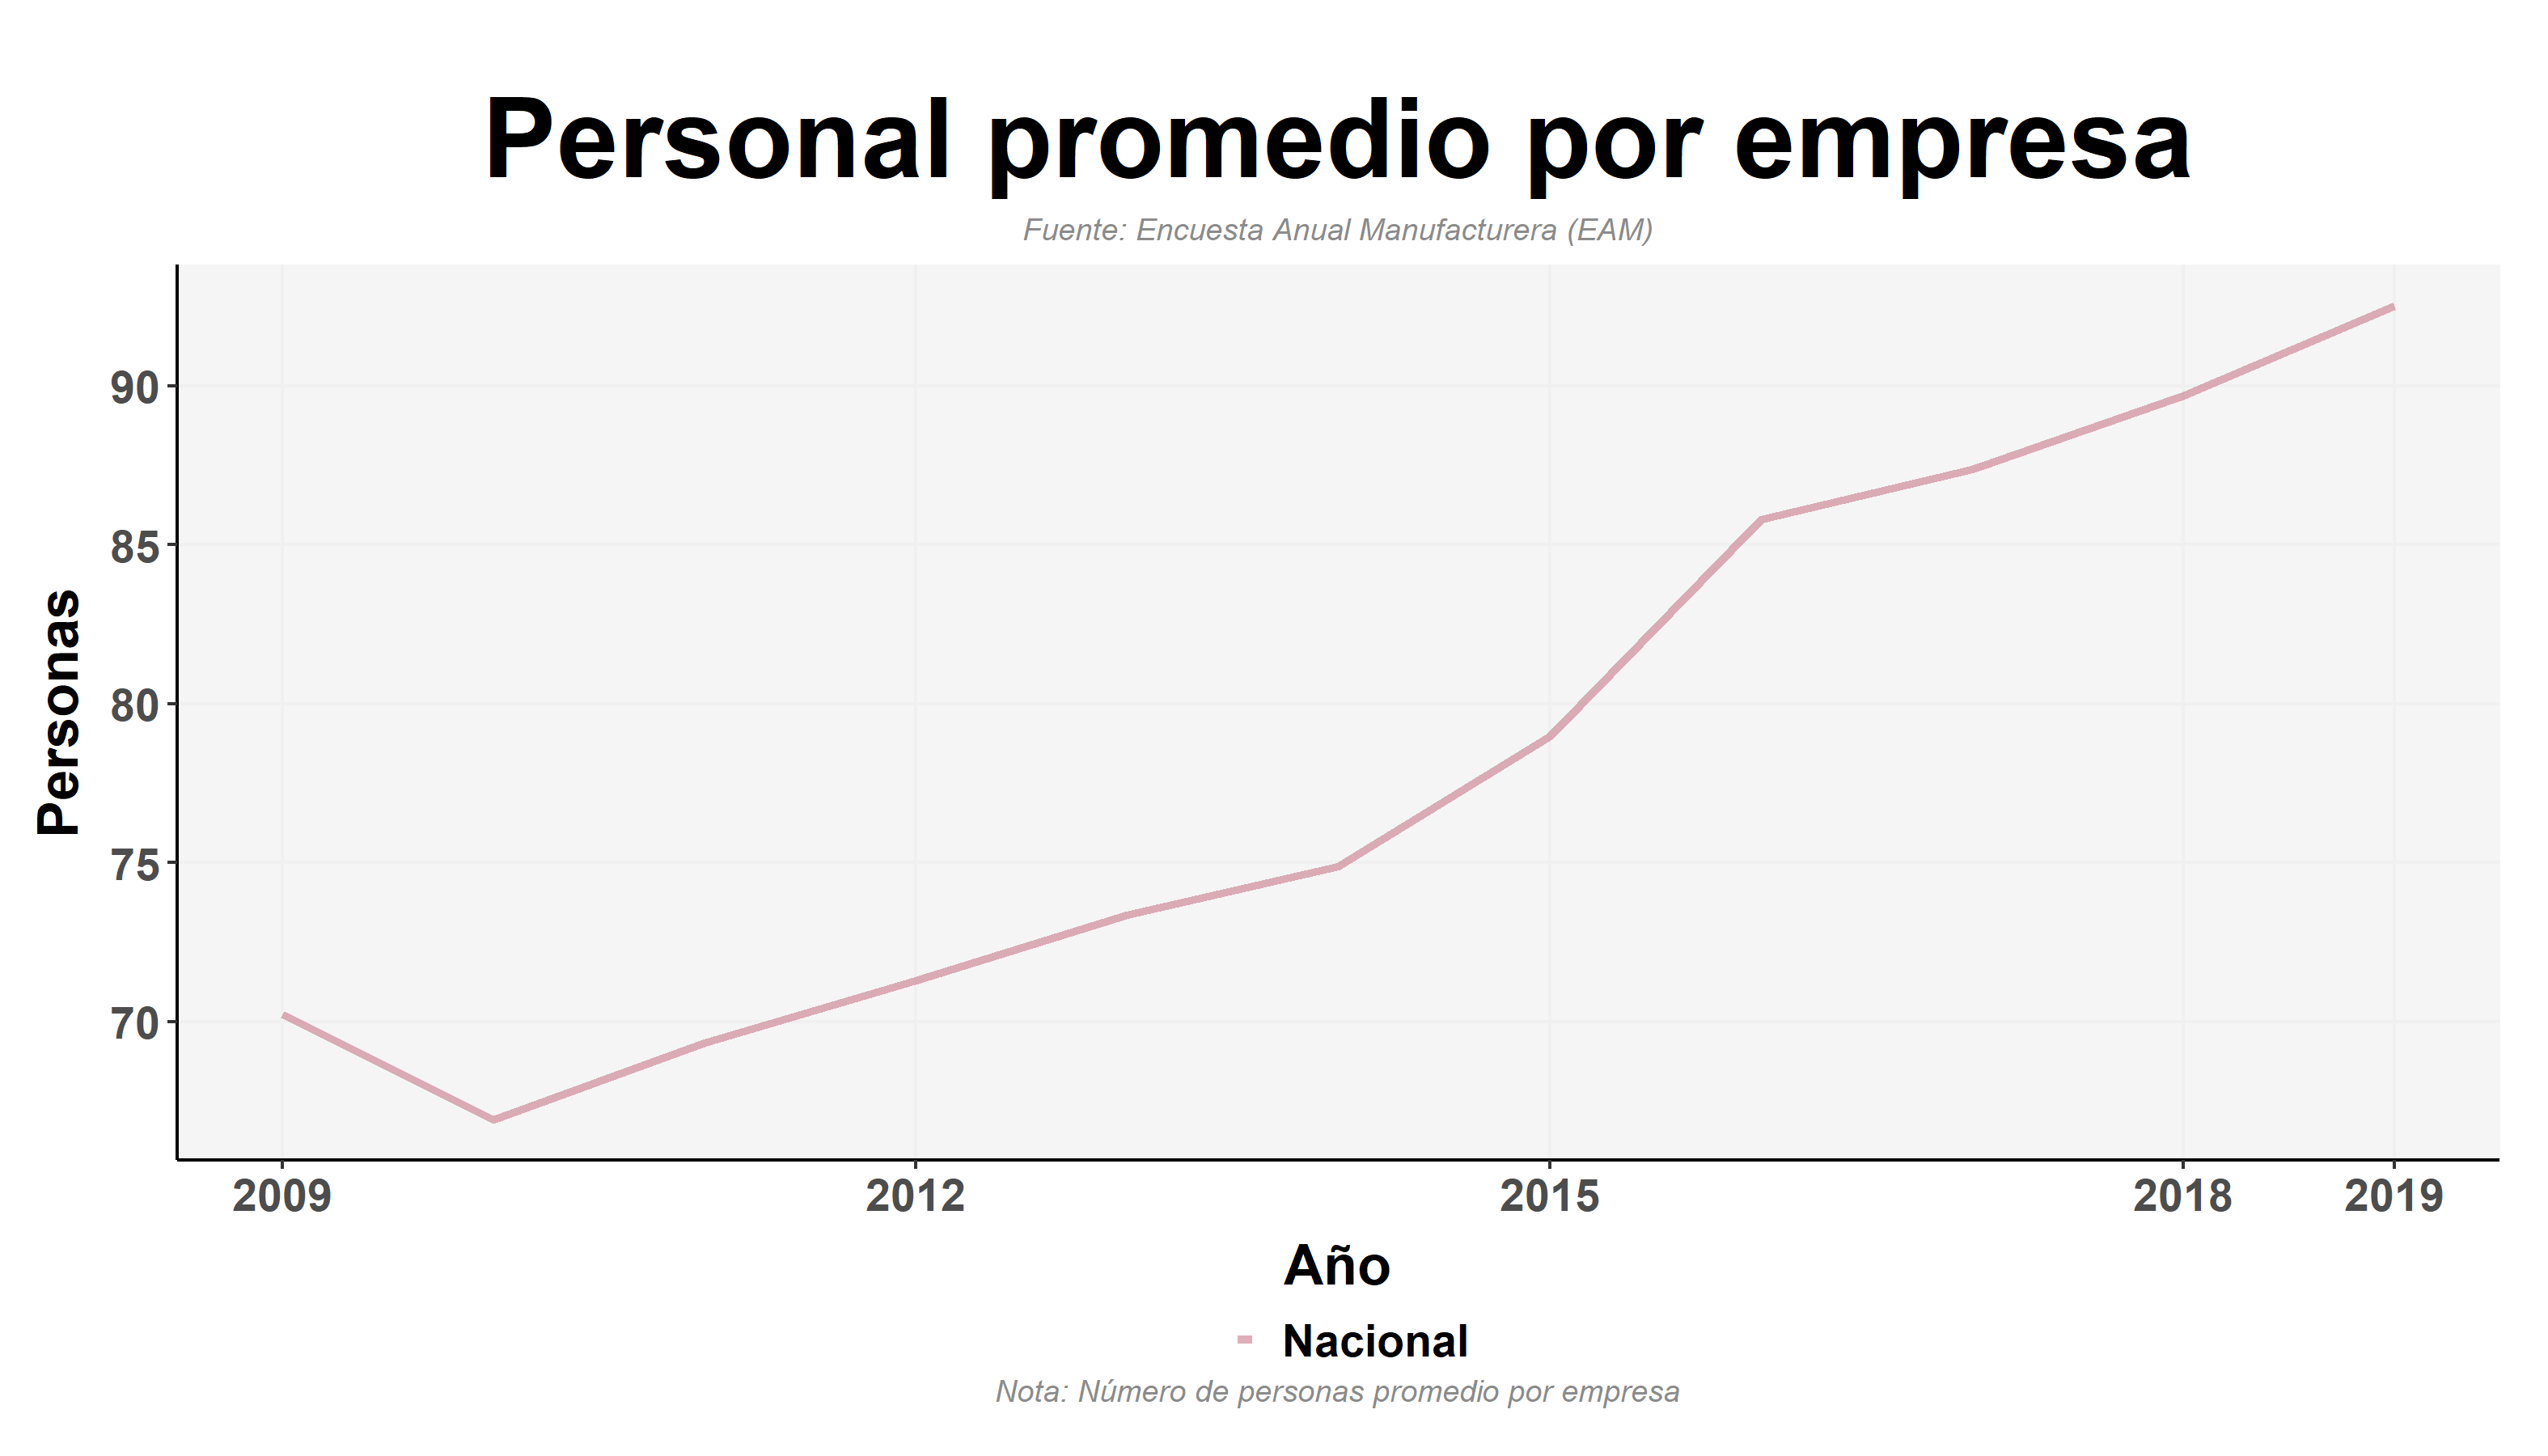
\includegraphics[width=\textwidth,keepaspectratio]{img/var_251_trend.png}
        \end{center}
    \end{figure}
            \begin{itemize}
                    \item La clase alta es la que demuestra mayor variación entre los años para el nivel nacional.
                    \item La clase alta presentó un decrecimiento después de 2014 hasta el 2017, repitiéndose en el 2020 donde cae abruptamente.
                    \item Para 2020 se registraron niveles menores comparado con los del 2012.
                    \end{itemize}

%%%% Include figures
    \begin{figure}[H]
        \caption{Población por clase social - Clase alta por zonas \label{map_result_2} }
        \begin{center}
        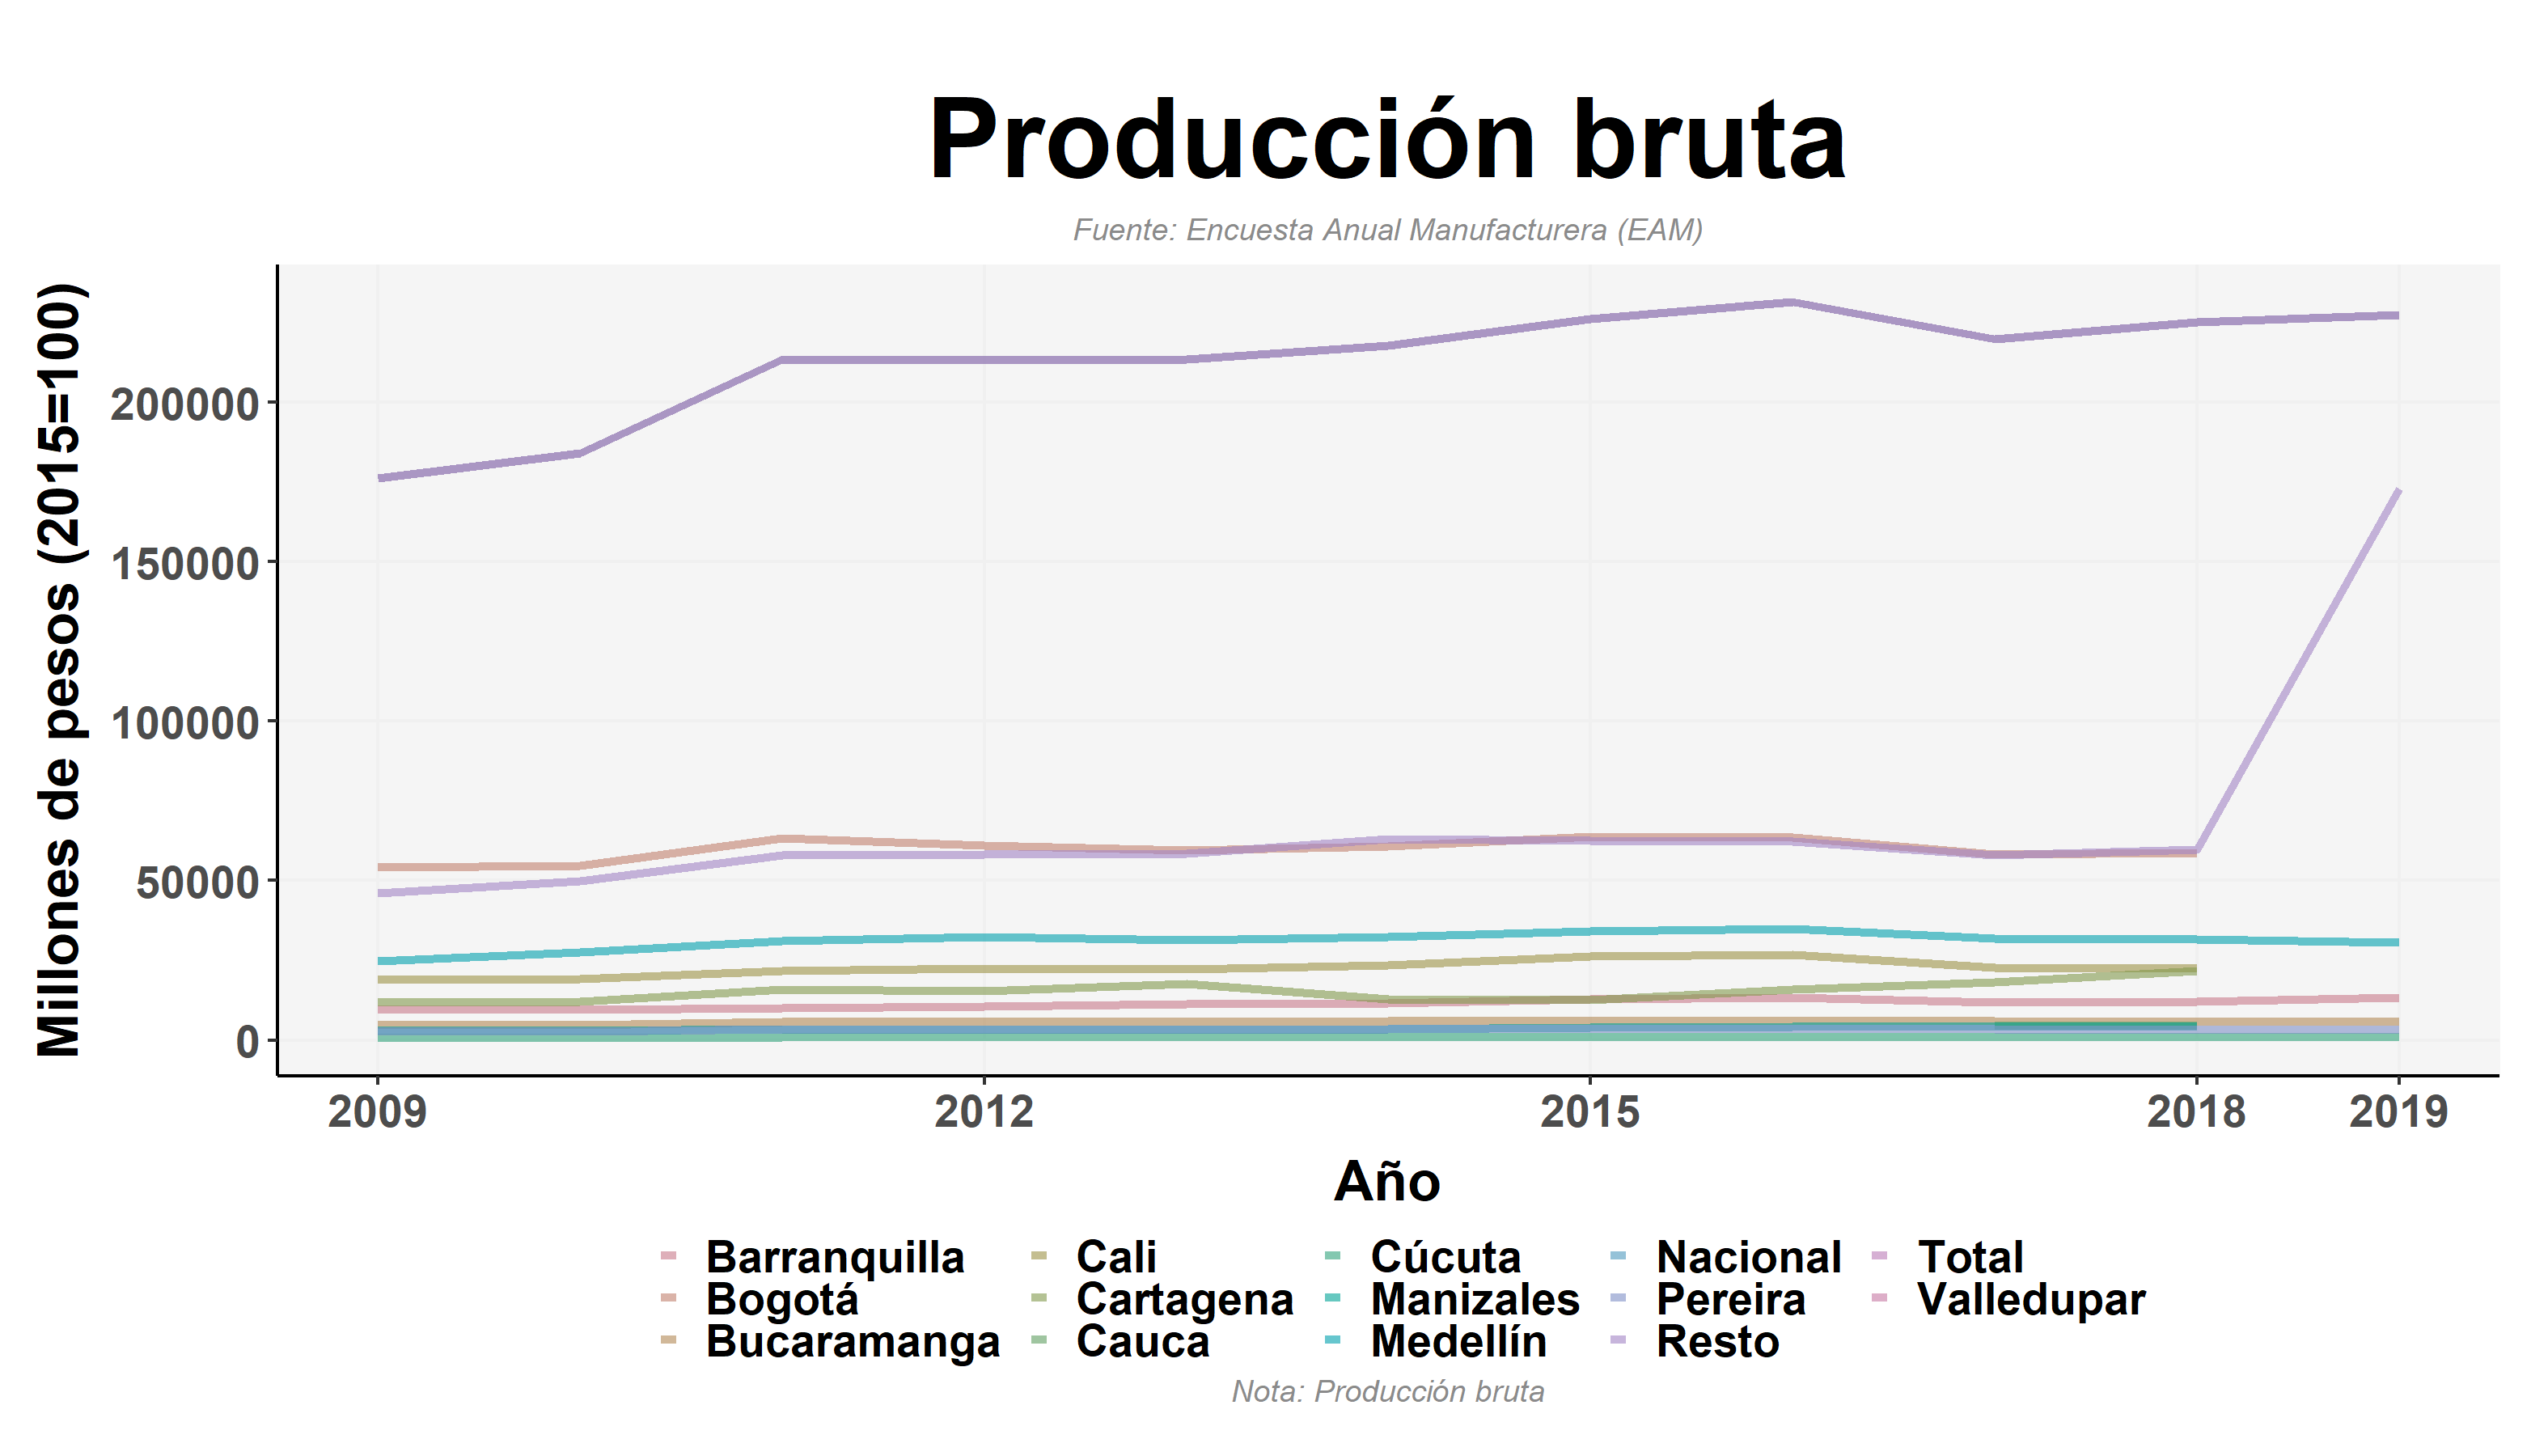
\includegraphics[width=\textwidth,keepaspectratio]{img/var_252_trend.png}
        \end{center}
    \end{figure}
            \begin{itemize}
                    \item Los centros poblados y el rural disperso presentan un crecimiento de la clase alta a lo largo del tiempo pero está por debajo del 1\% de la población.
                    \item Las cabeceras y a nivel nacional se presenta la misma tendencia, presentando para el 2020 niveles menores a los registrados en el 2012.
                    \end{itemize}

        \subsubsection{Pobreza Extrema}

%%%% Include figures
    \begin{figure}[H]
        \caption{Pobreza extrema por ciudades - 2012 VS 2020 \label{map_result_2} }
        \begin{center}
        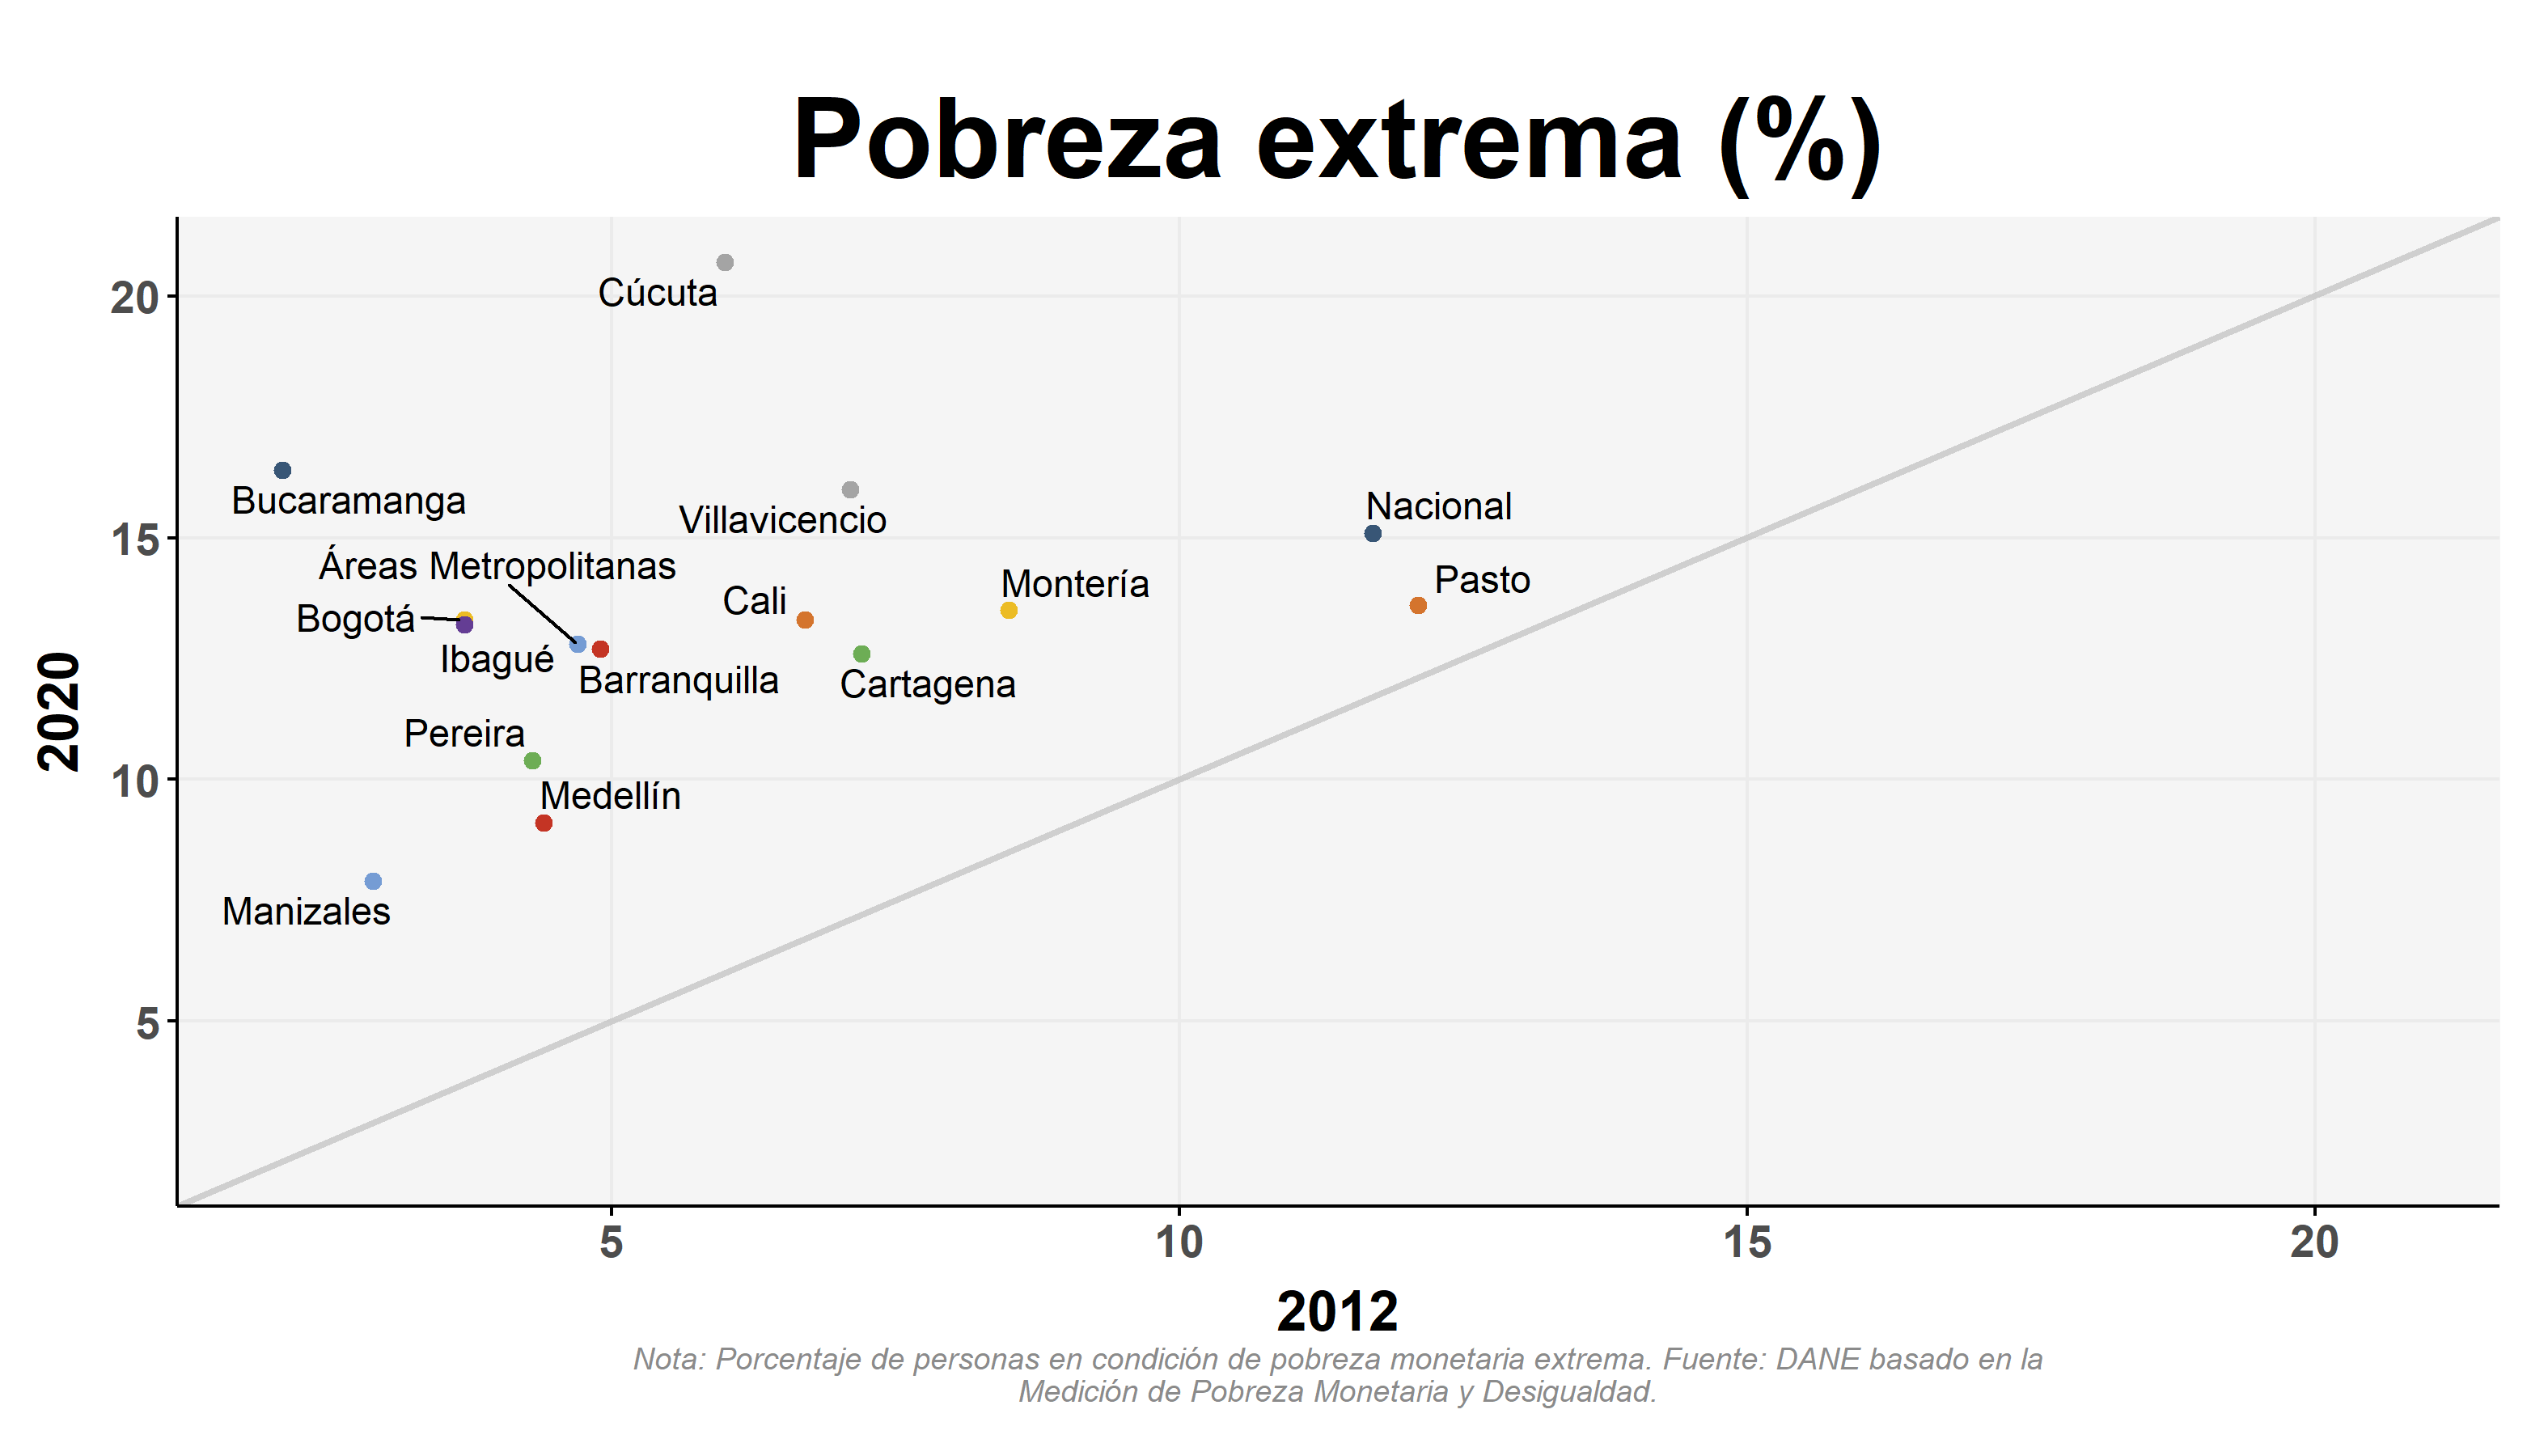
\includegraphics[width=\textwidth,keepaspectratio]{img/var_257_scatter_time.png}
        \end{center}
    \end{figure}
            \begin{itemize}
                    \item Todas las ciudades principales presentaron mayores niveles de pobreza extrema en 2020 que los registrados para 2012.
                    \item Bucaramanga pasó de ser la ciudad con menor nivel de pobreza extrema para 2012 a la segunda con mayor nivel en el 2020.
                    \item Cúcuta pasó de estar en el medio de las ciudades a ser la de mayor nivel de pobreza monetaria.
                    \item Pasto es la única ciudad que mantuvo los niveles de pobreza extrema en 2020 más cercanos a los de 2012, aunque superiores.
                    \item Entre las ciudades extremas hay una diferencia aproximadamente del 12\% (Manizales - Cúcuta).
                    \end{itemize}

%%%% Include figures
    \begin{figure}[H]
        \caption{Pobreza extrema por departamentos - 2012 VS 2020 \label{map_result_2} }
        \begin{center}
        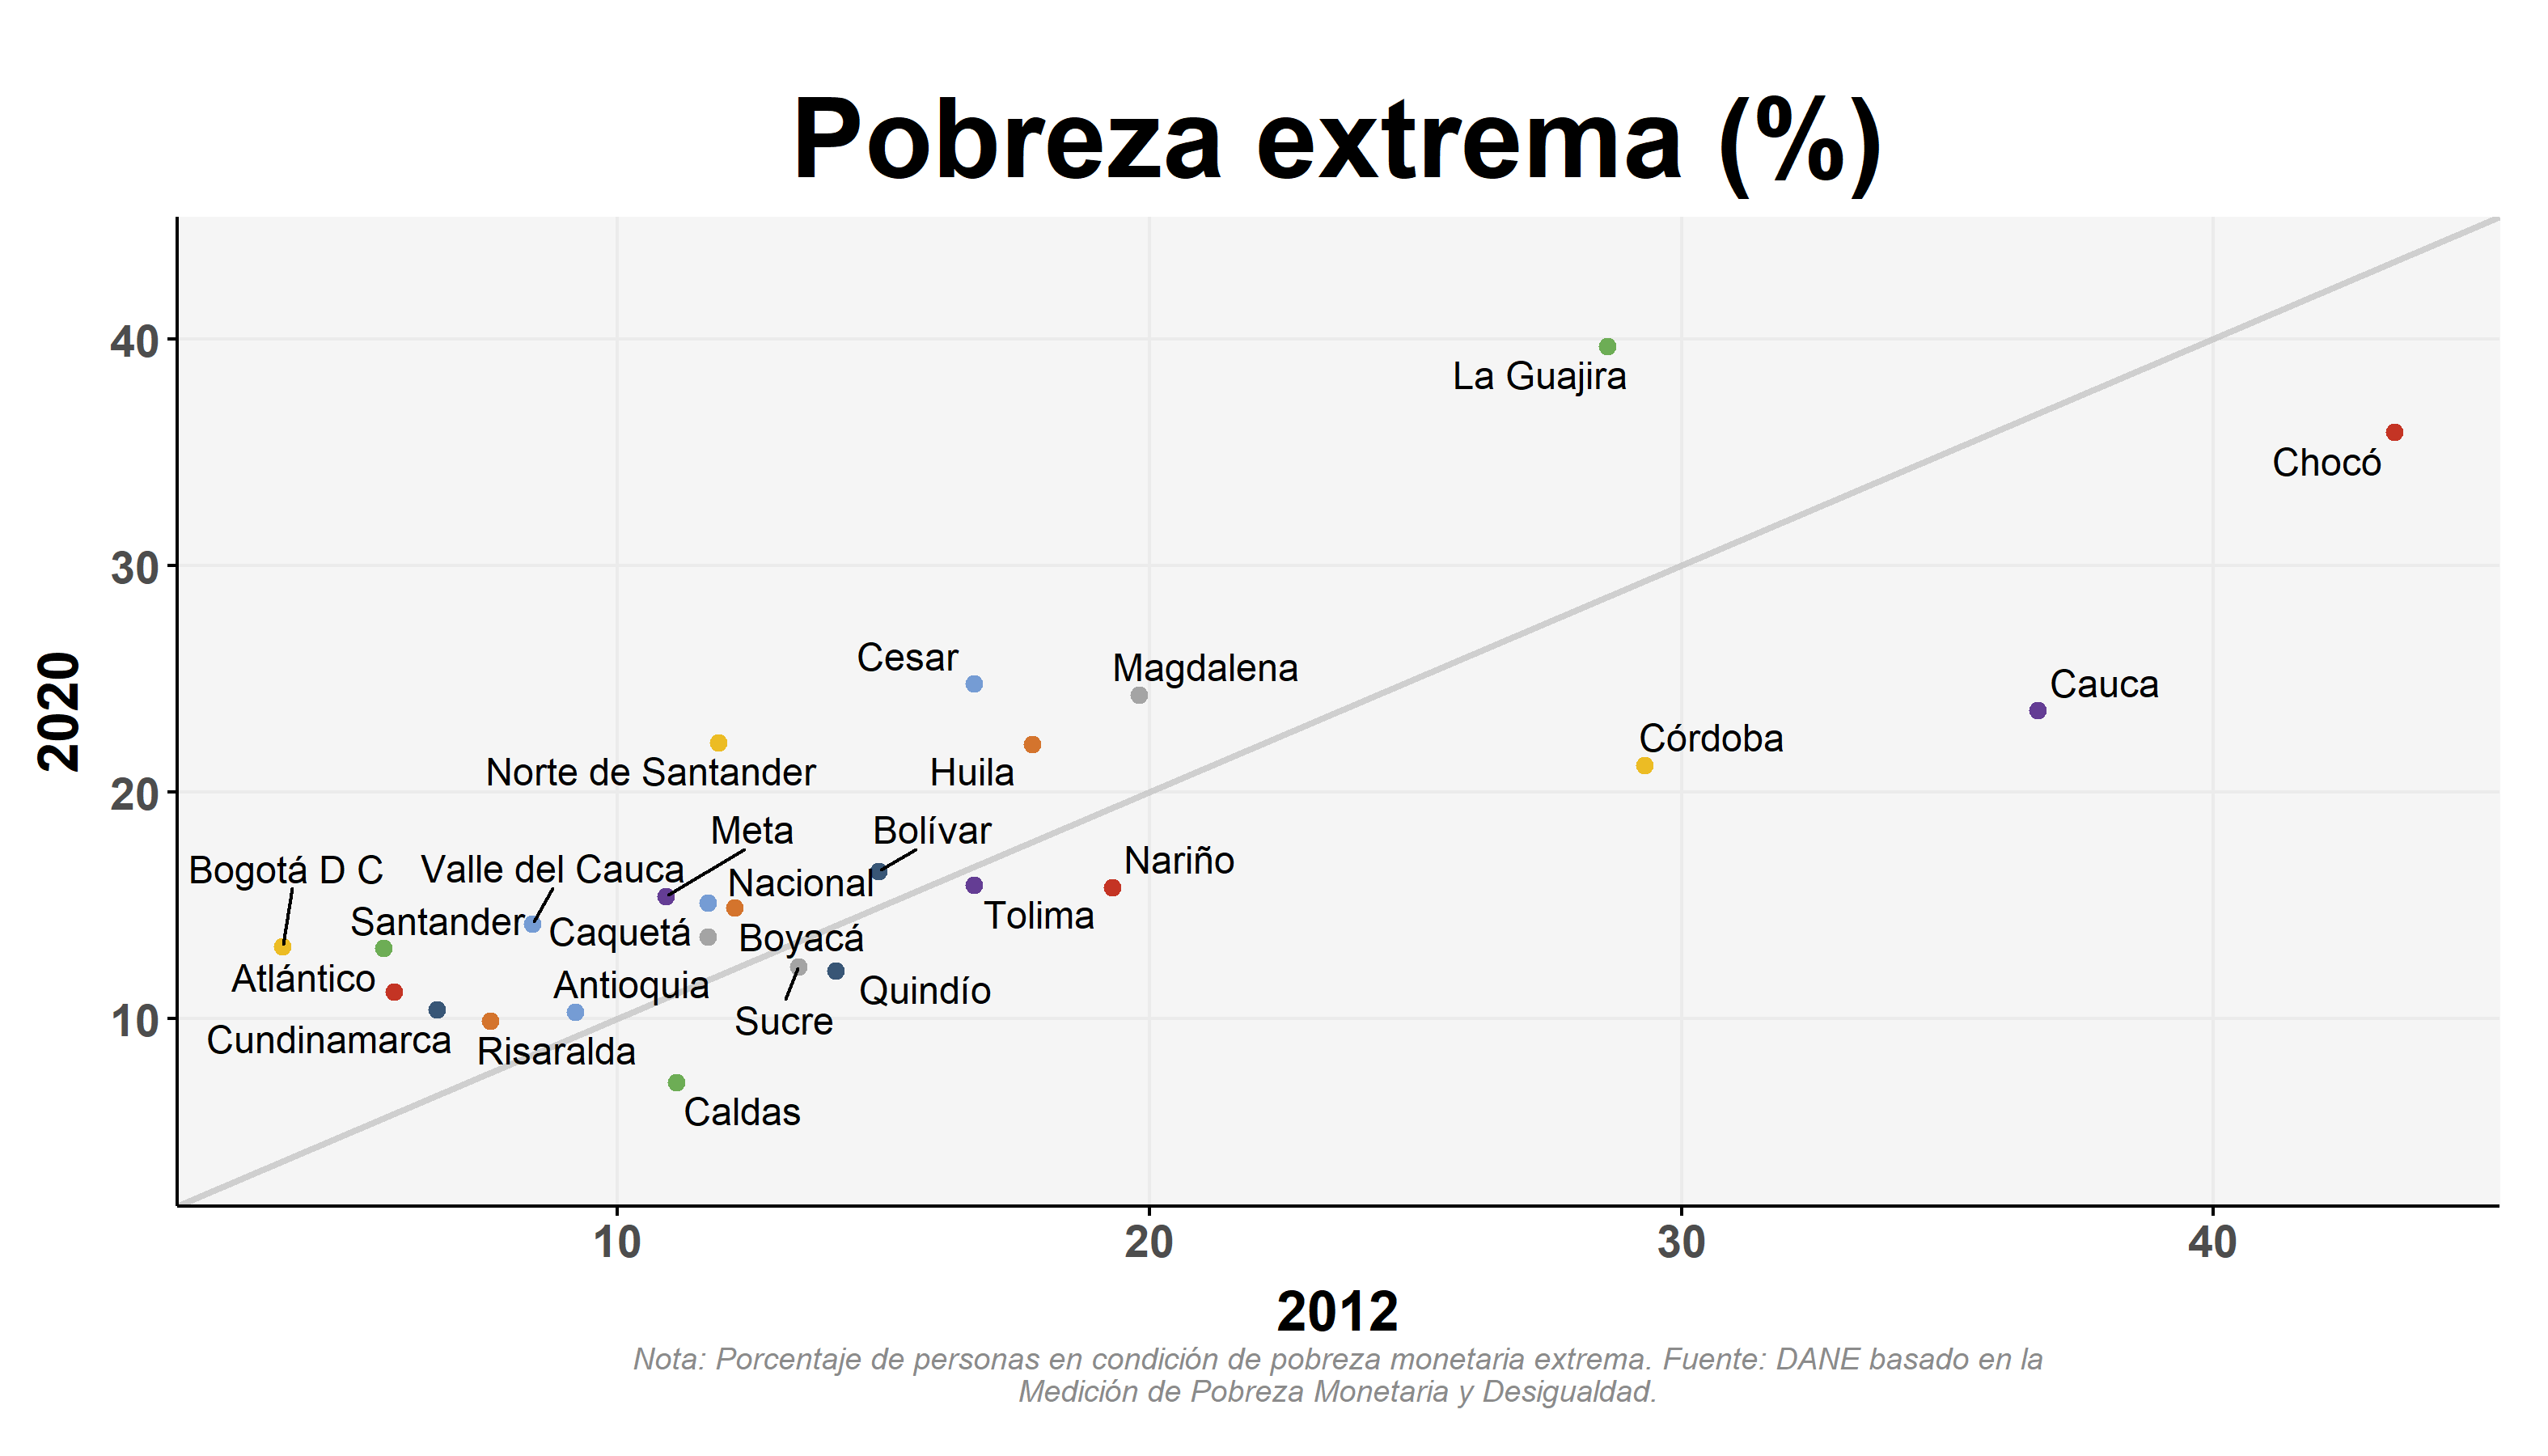
\includegraphics[width=\textwidth,keepaspectratio]{img/var_258_scatter_time.png}
        \end{center}
    \end{figure}
            \begin{itemize}
                    \item Departamentos como Chocó, Cauca, Córdoba, Caldas y Nariño presentaron mejoras significativas para el 2020 comparado con los presentados en 2012.
                    \item Antioquia, Sucre y Tolima mantuvieron niveles de pobreza extrema similares entre 2012 y 2020.
                    \item Gran parte de los departamentos obtuvieron registros superiores para 2020 comparado con los del 2012, la mayoría se concentran entre el 10 y 20\% de pobreza extrema.
                    \item La Guajira y Chocó son los departamentos con los mayores niveles de pobreza extrema con una diferencia por encima del 10\% con el tercer departamento en fila.
                    \end{itemize}

%%%% Include figures
    \begin{figure}[H]
        \caption{Pobreza extrema por departamentos - Cambio porcentual entre 2012 y 2020 \label{map_result_2} }
        \begin{center}
        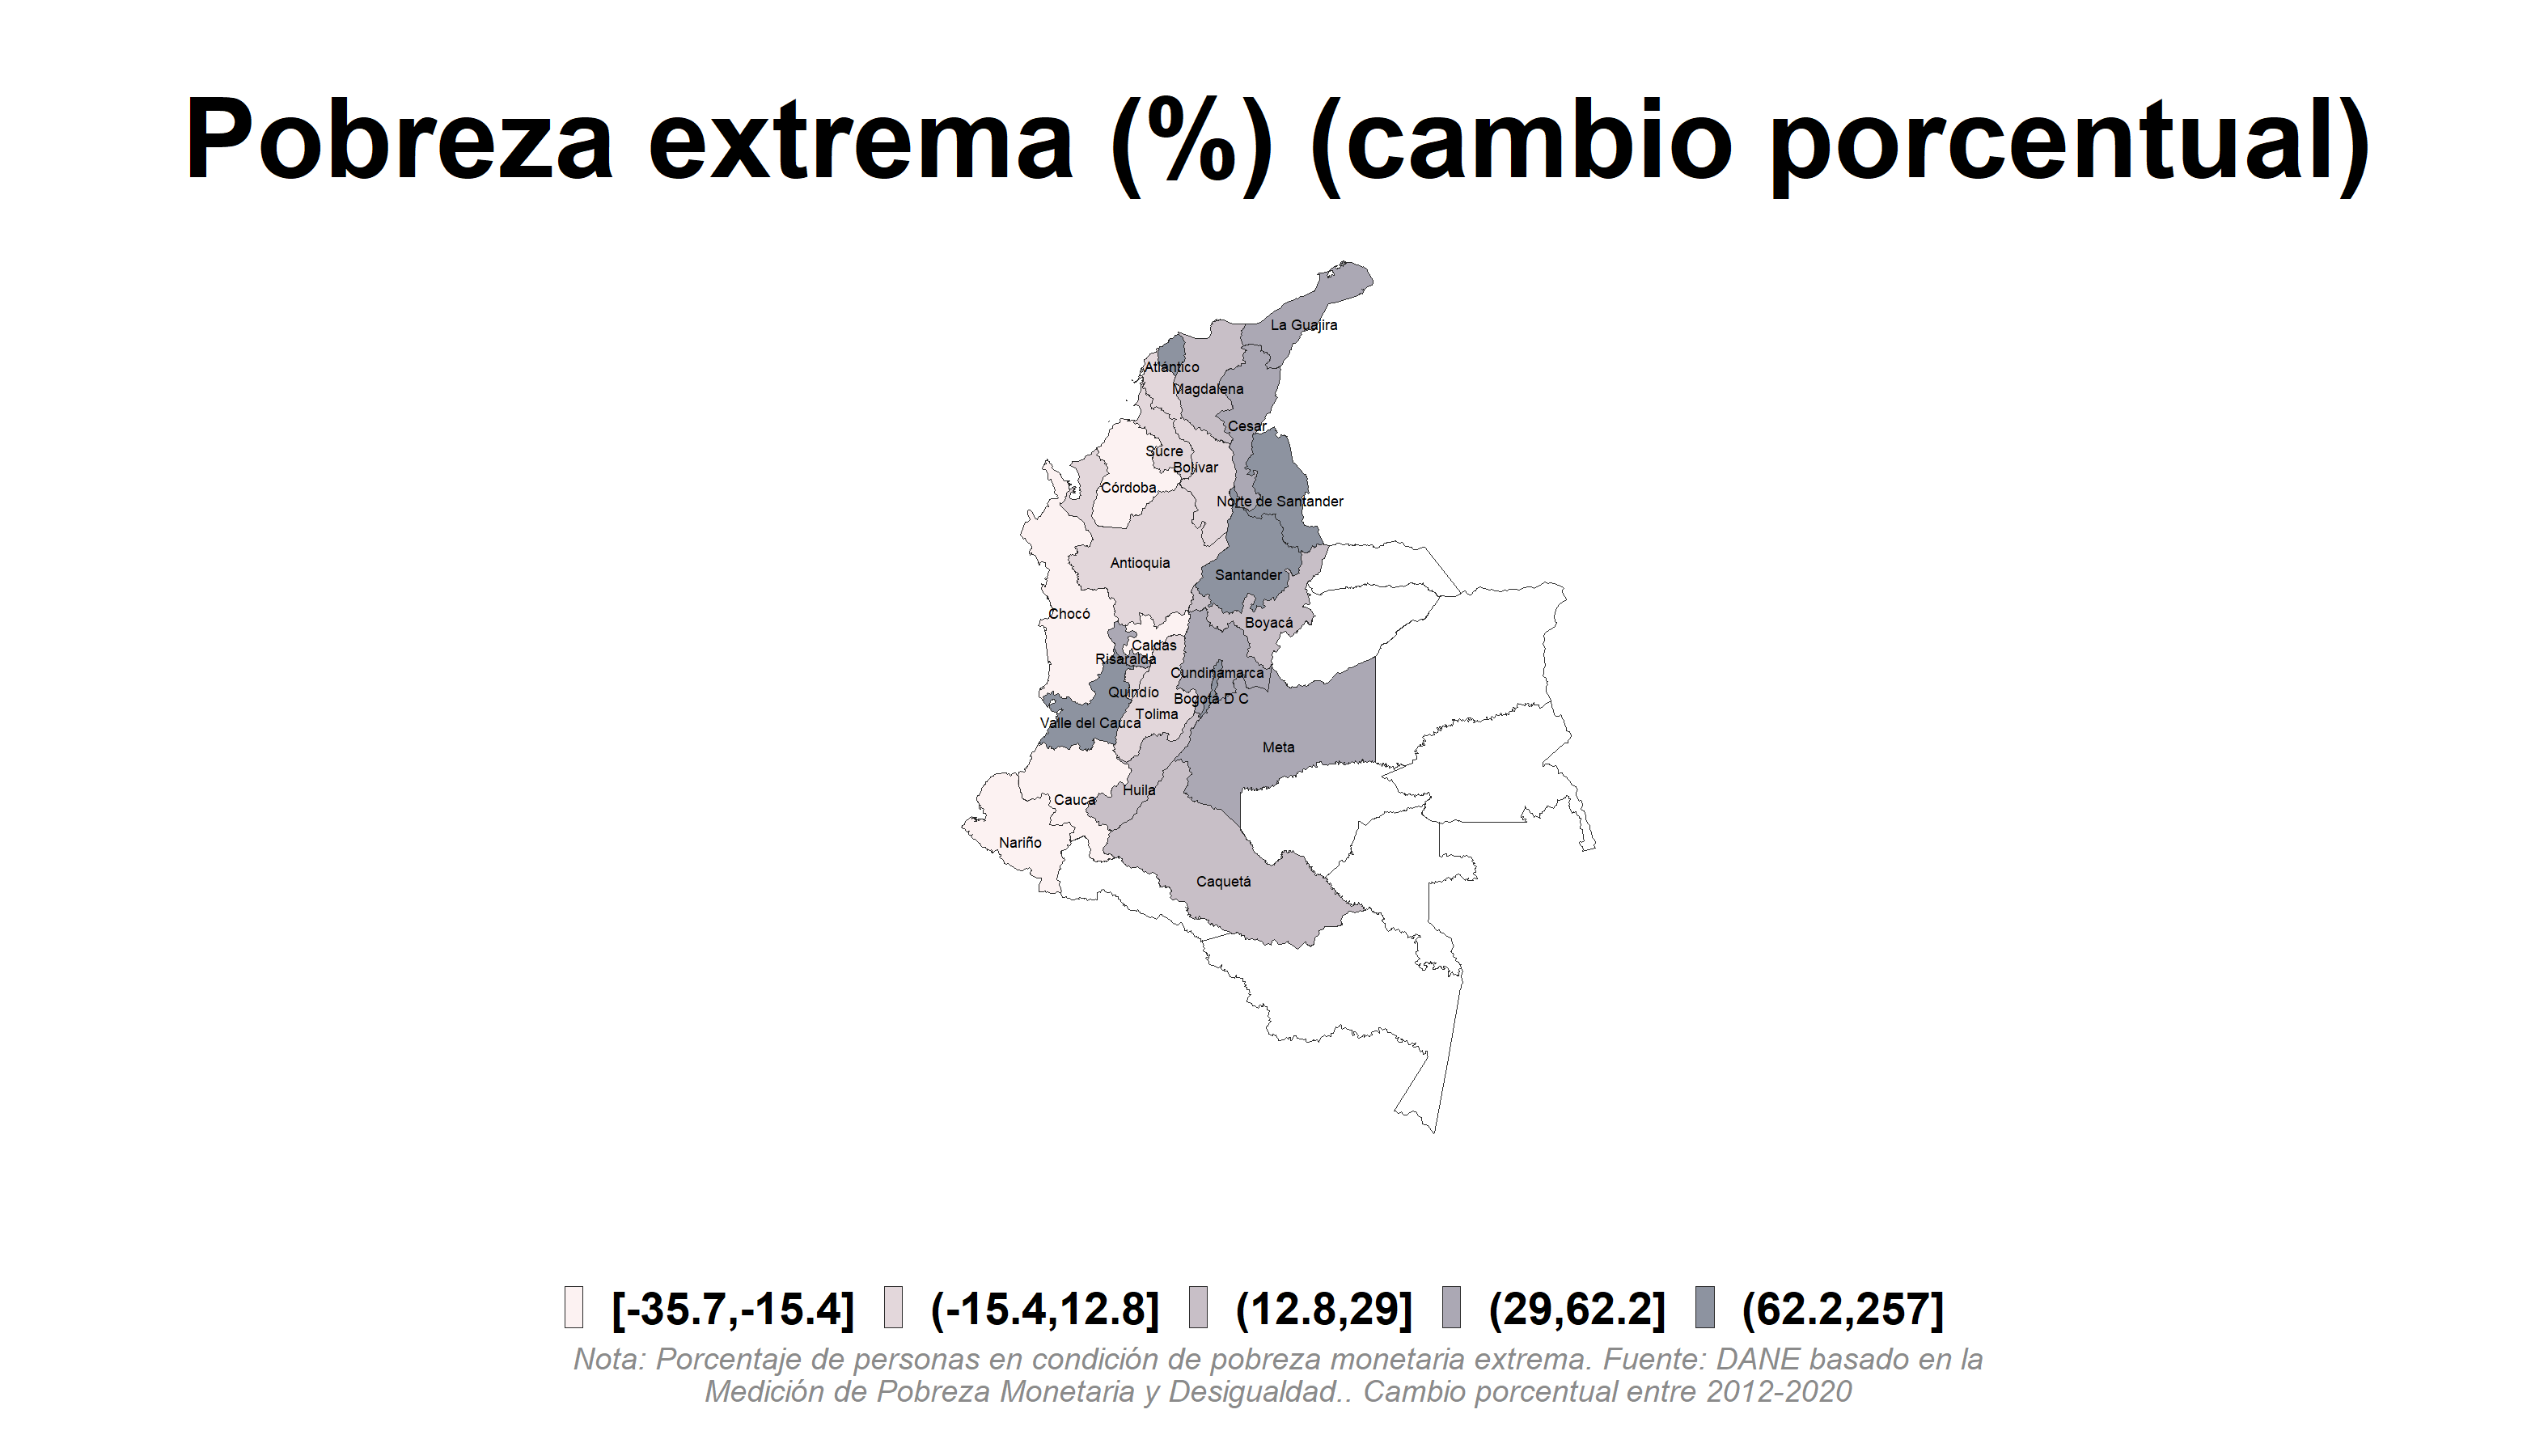
\includegraphics[width=\textwidth,keepaspectratio]{img/var_258_map_change.png}
        \end{center}
    \end{figure}
            \begin{itemize}
                    \item Chocó, Cauca, Nariño, Córdoba y Caldas muestran mejoras significativas entre los dos años.
                    \item Santander, Norte de Santander, Valle, Atlántico y Bogotá son los que presentan los mayores rangos de aumento de pobreza extrema entre los 2 años.
                    \end{itemize}

%%%% Include figures
    \begin{figure}[H]
        \caption{Pobreza extrema por zonas y nacional \label{map_result_2} }
        \begin{center}
        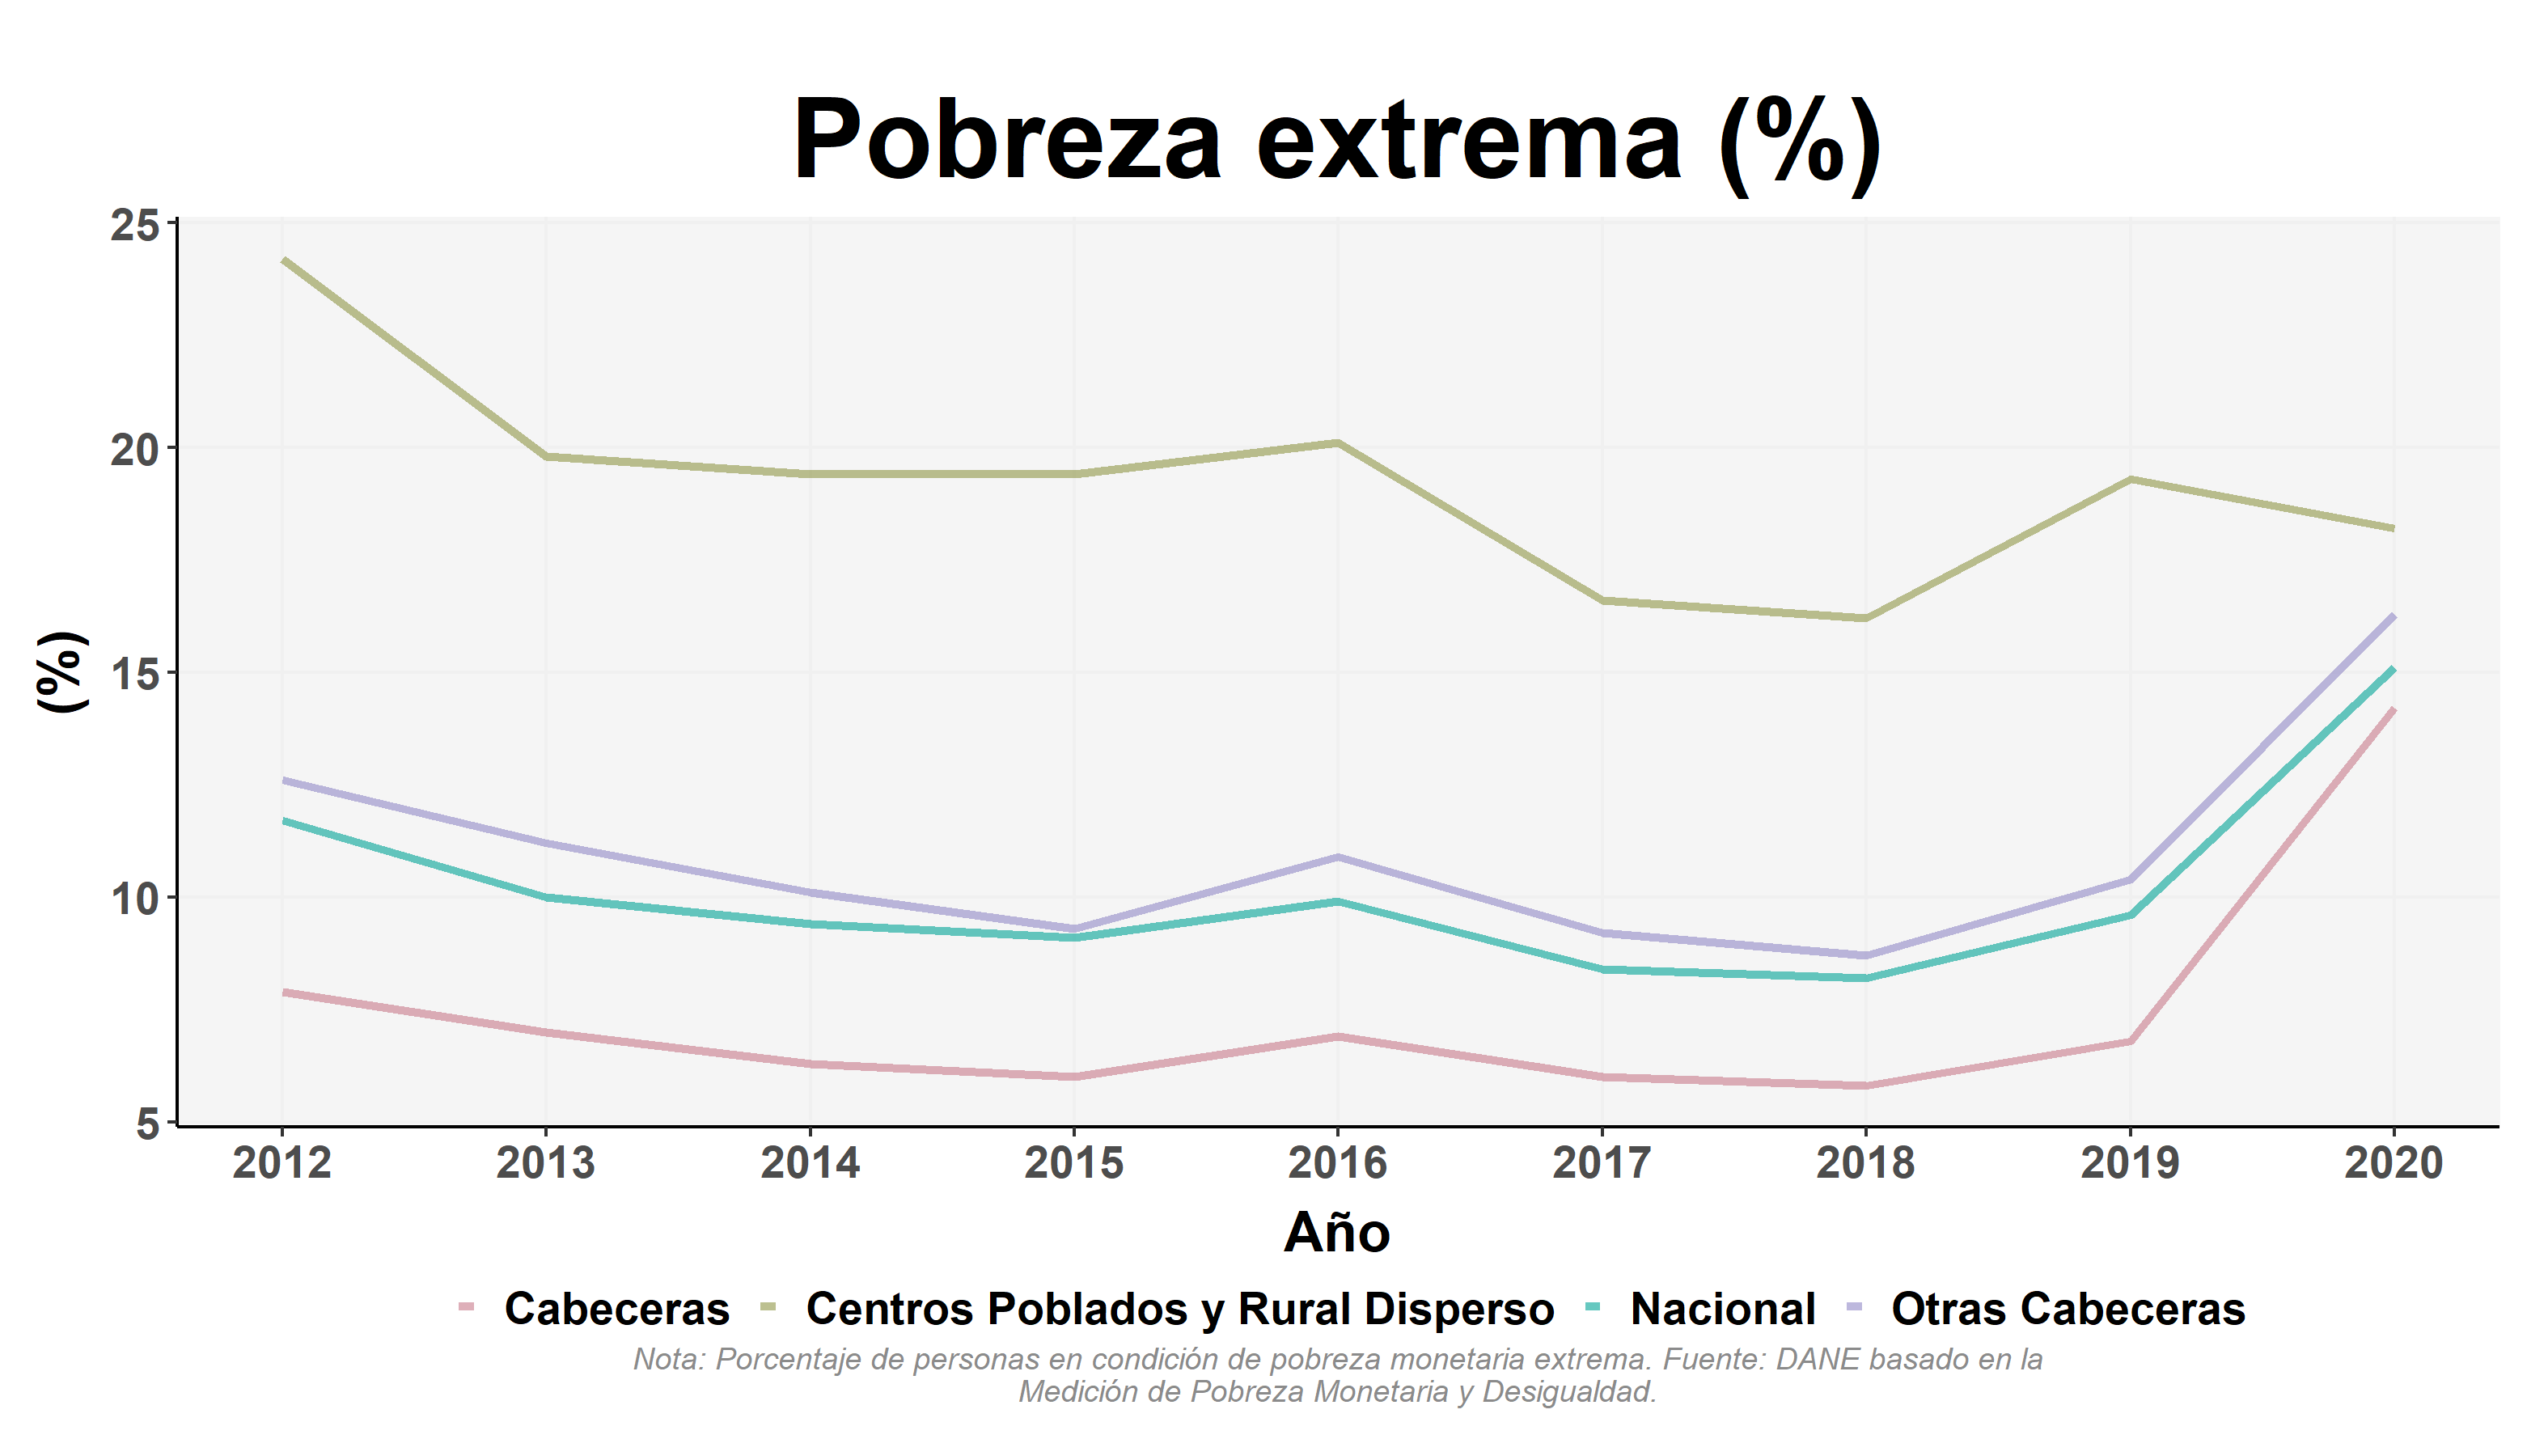
\includegraphics[width=\textwidth,keepaspectratio]{img/var_260_trend.png}
        \end{center}
    \end{figure}
            \begin{itemize}
                    \item Los niveles de pobreza extrema estaban disminuyendo, con un leve pico en 2016, hasta 2018.
                    \item Desde el 2019 se inicio un crecimiento, intensificado en el 2020 pero caso contrario con los centros poblados y rural donde en el 2020 disminuyó.
                    \item Se disminuyó la brecha entre a zona rural y las otras zonas, acercándose para el 2020.
                    \item Para las cabeceras, a nivel nacional y las otras cabeceras se registraron para 2020 valores superiores que los del 2012, caso contrario con las zonas rurales. 
                    \end{itemize}

\subsubsection{Pobreza Monetaria}

%%%% Include figures
    \begin{figure}[H]
        \caption{Pobreza monetaria por ciudades - 2012 VS 2020 \label{map_result_2} }
        \begin{center}
        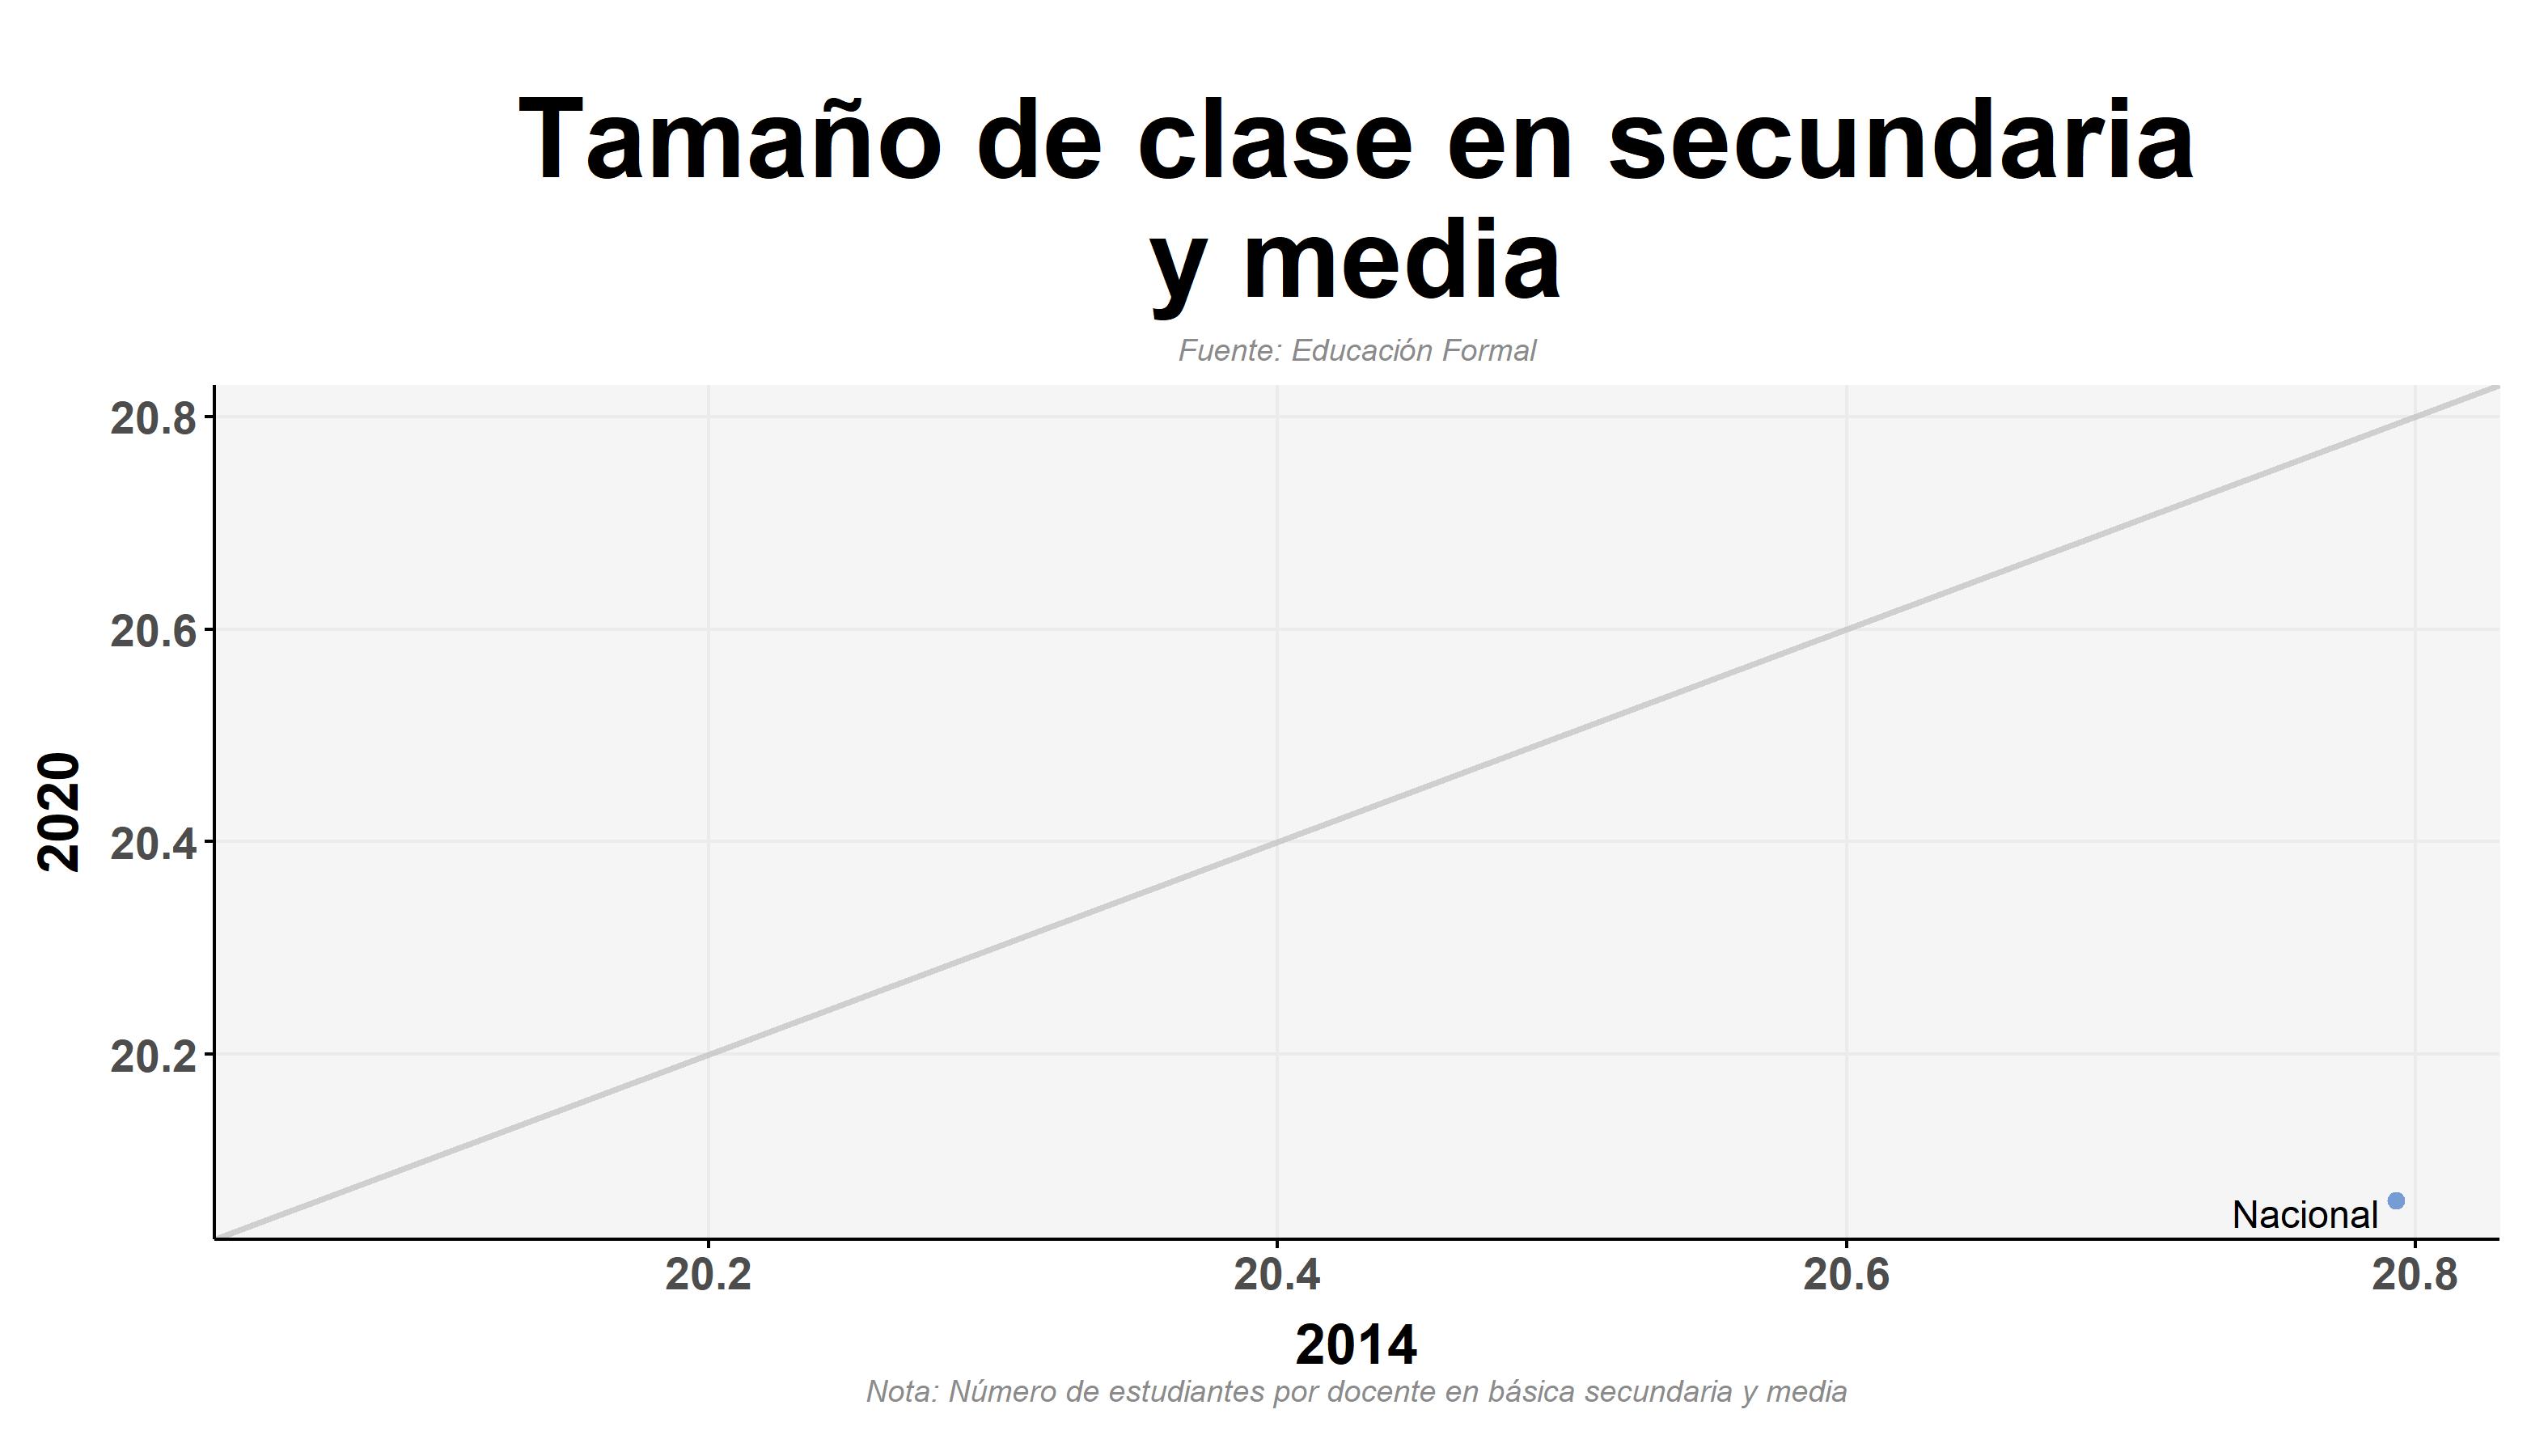
\includegraphics[width=\textwidth,keepaspectratio]{img/var_261_scatter_time.png}
        \end{center}
    \end{figure}
            \begin{itemize}
                    \item Pasto es la única ciudad que mejoró sus niveles de pobreza monetaria en 2020 con respecto al 2012, las demás ciudades tuvieron valores más altos.
                    \item Todas las ciudades están por encima del 30\% de la población en pobreza monetaria, Cúcuta es la única que pasa del 50\% de su población viviendo con pobreza monetaria.
                    \item Bucaramanga paso de ser la ciudad con el menor nivel de pobreza monetaria en 2012, cerca del 20\%, a ser la cuarta ciudad con mayor nivel de población en pobreza monetaria con niveles por encima del 45\%.
                    \item Entre las ciudades extremo hay una diferencia aproximada del 20\% (Manizales - Cúcuta).
                    \end{itemize}

%%%% Include figures
    \begin{figure}[H]
        \caption{Pobreza monetaria por departamentos - 2012 VS 2020 \label{map_result_2} }
        \begin{center}
        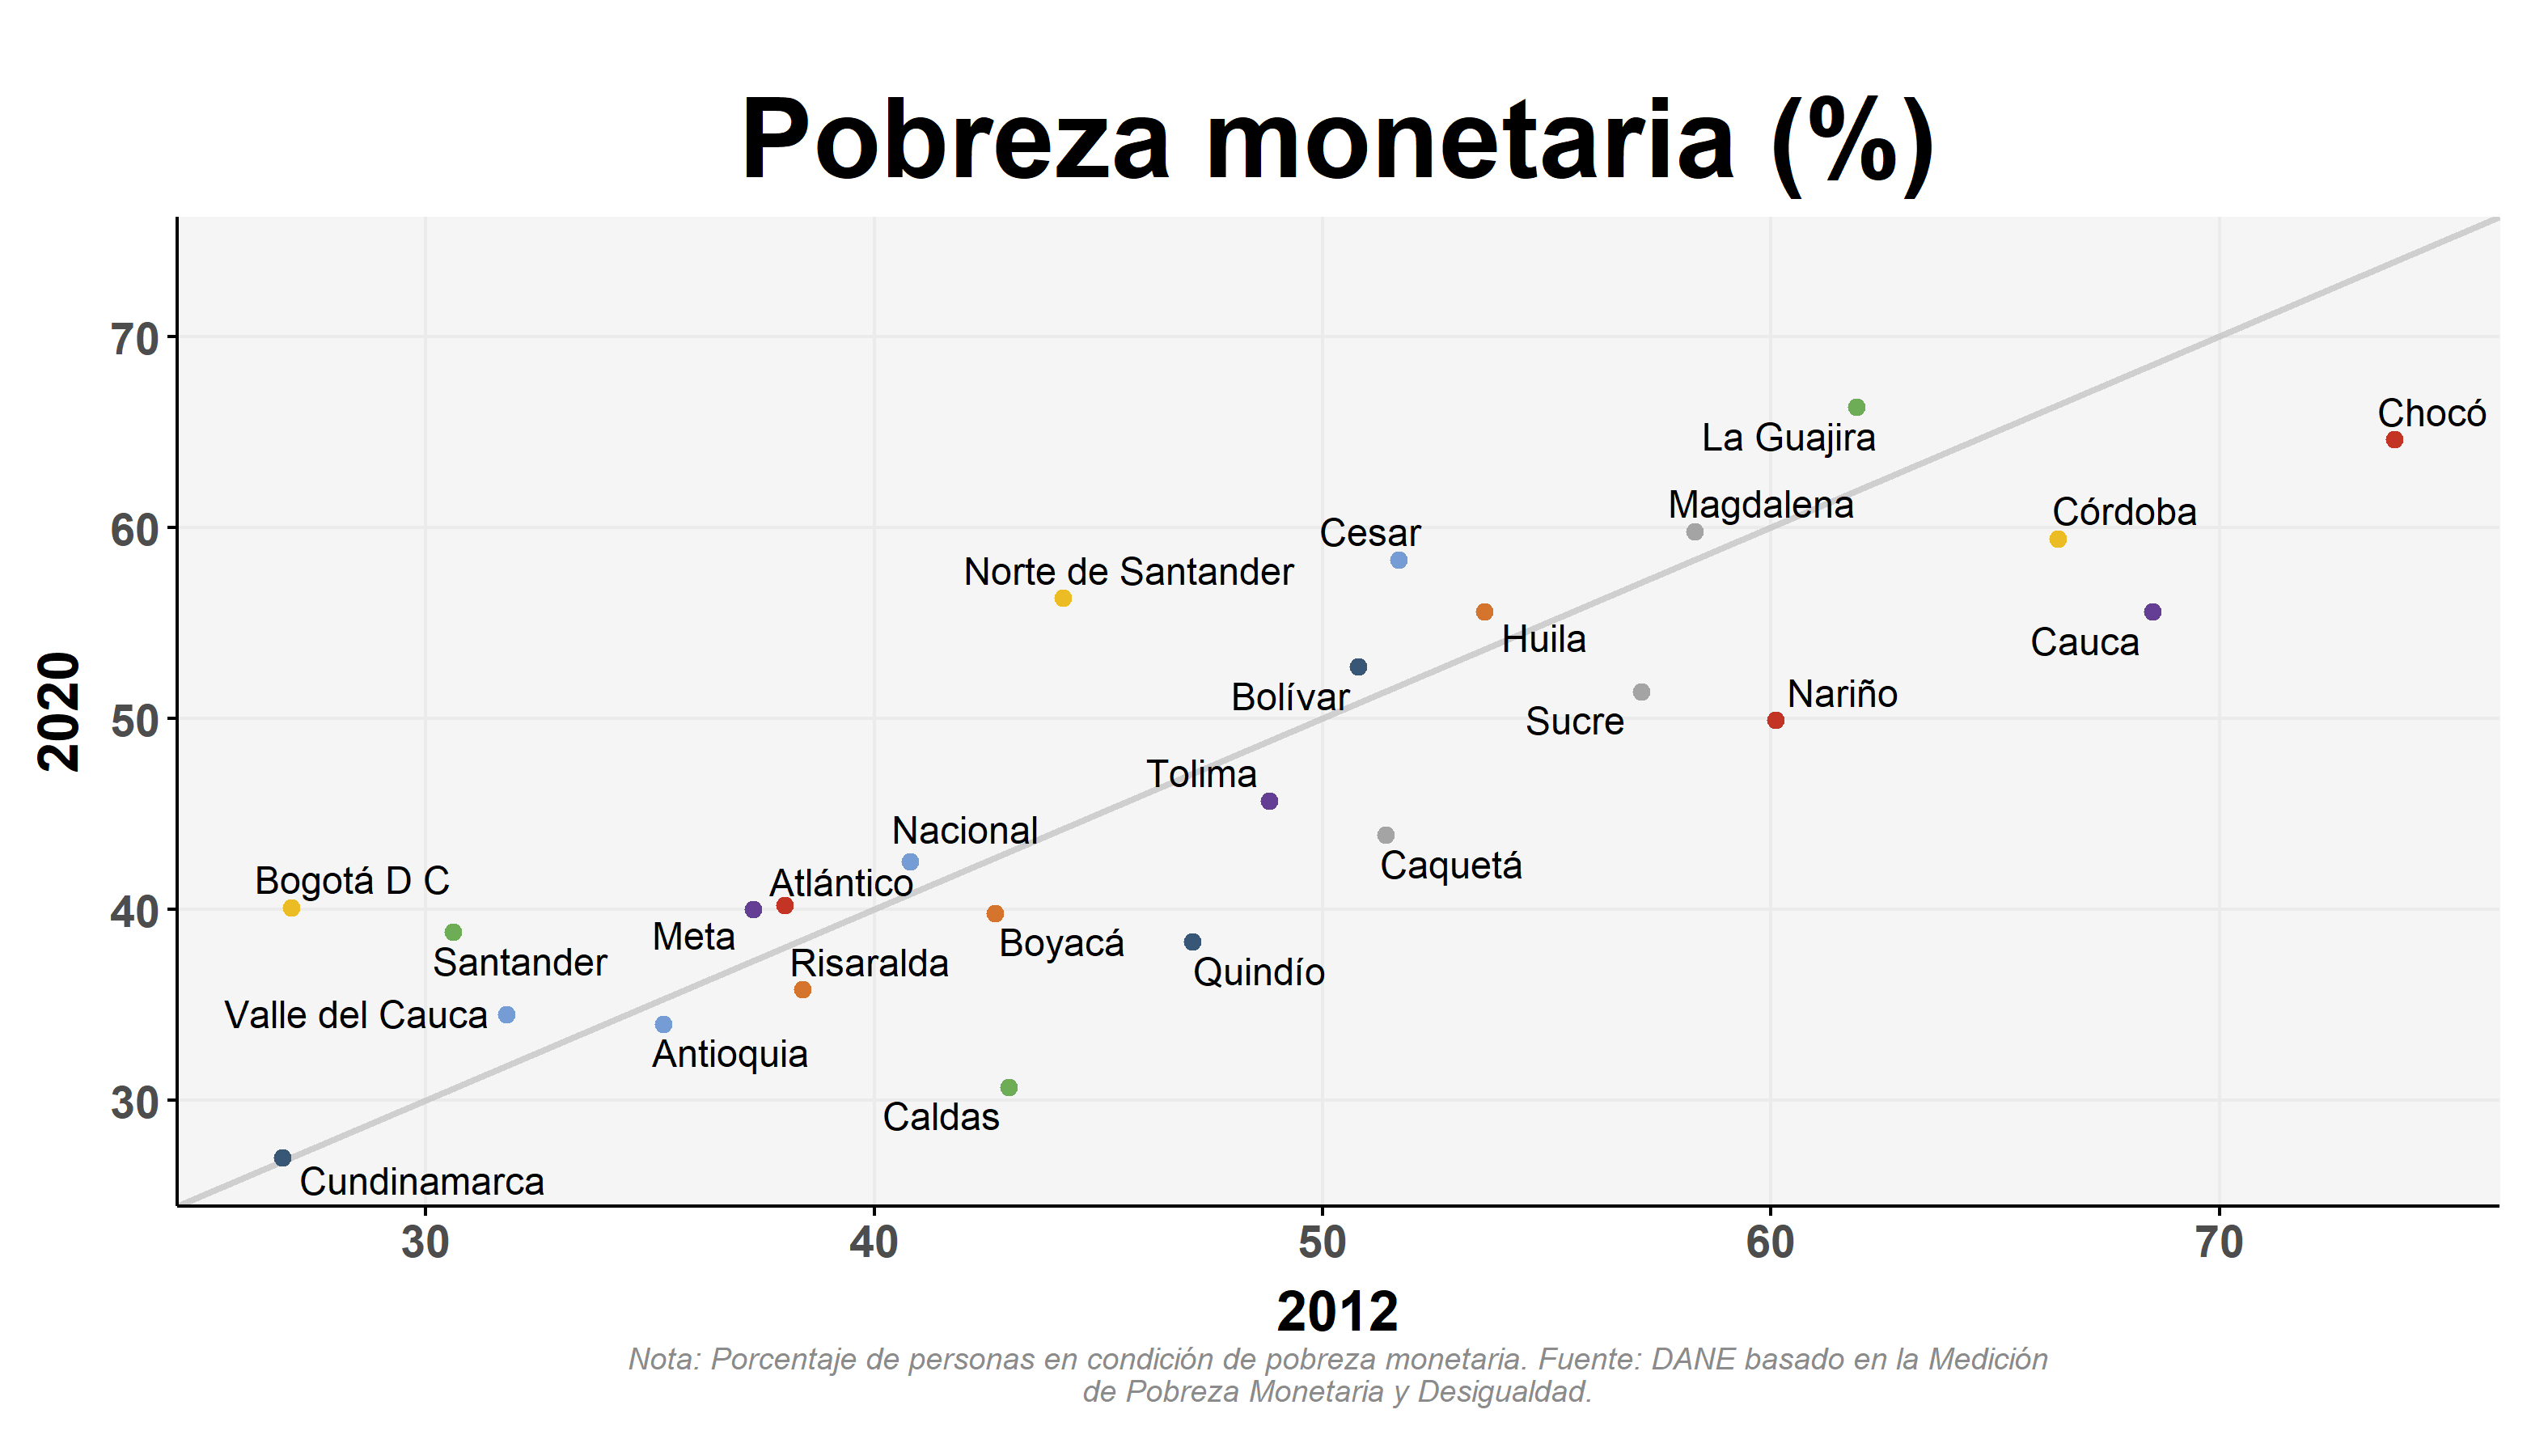
\includegraphics[width=\textwidth,keepaspectratio]{img/var_262_scatter_time.png}
        \end{center}
    \end{figure}
            \begin{itemize}
                    \item La mitad de los departamentos tuvieron mejoras en el 2020 con respecto al 2012.
                    \item Chocó a pesar de haber mejorado se mantiene como el segundo dpto con mayor pobreza en 2020, en 2012 fue el primero.
                    \item La diferencia entre los dptos extremo es del aproximadamente el 40\% (Cundinamarca - La Guajira).
                    \item Vemos que la distribución de lugares no ha cambiado drásticamente y la de valores tienen una amplia distribución.
                    \end{itemize}

%%%% Include figures
    \begin{figure}[H]
        \caption{Pobreza monetaria por departamentos - Cambio porcentual entre 2012 y 2020 \label{map_result_2} }
        \begin{center}
        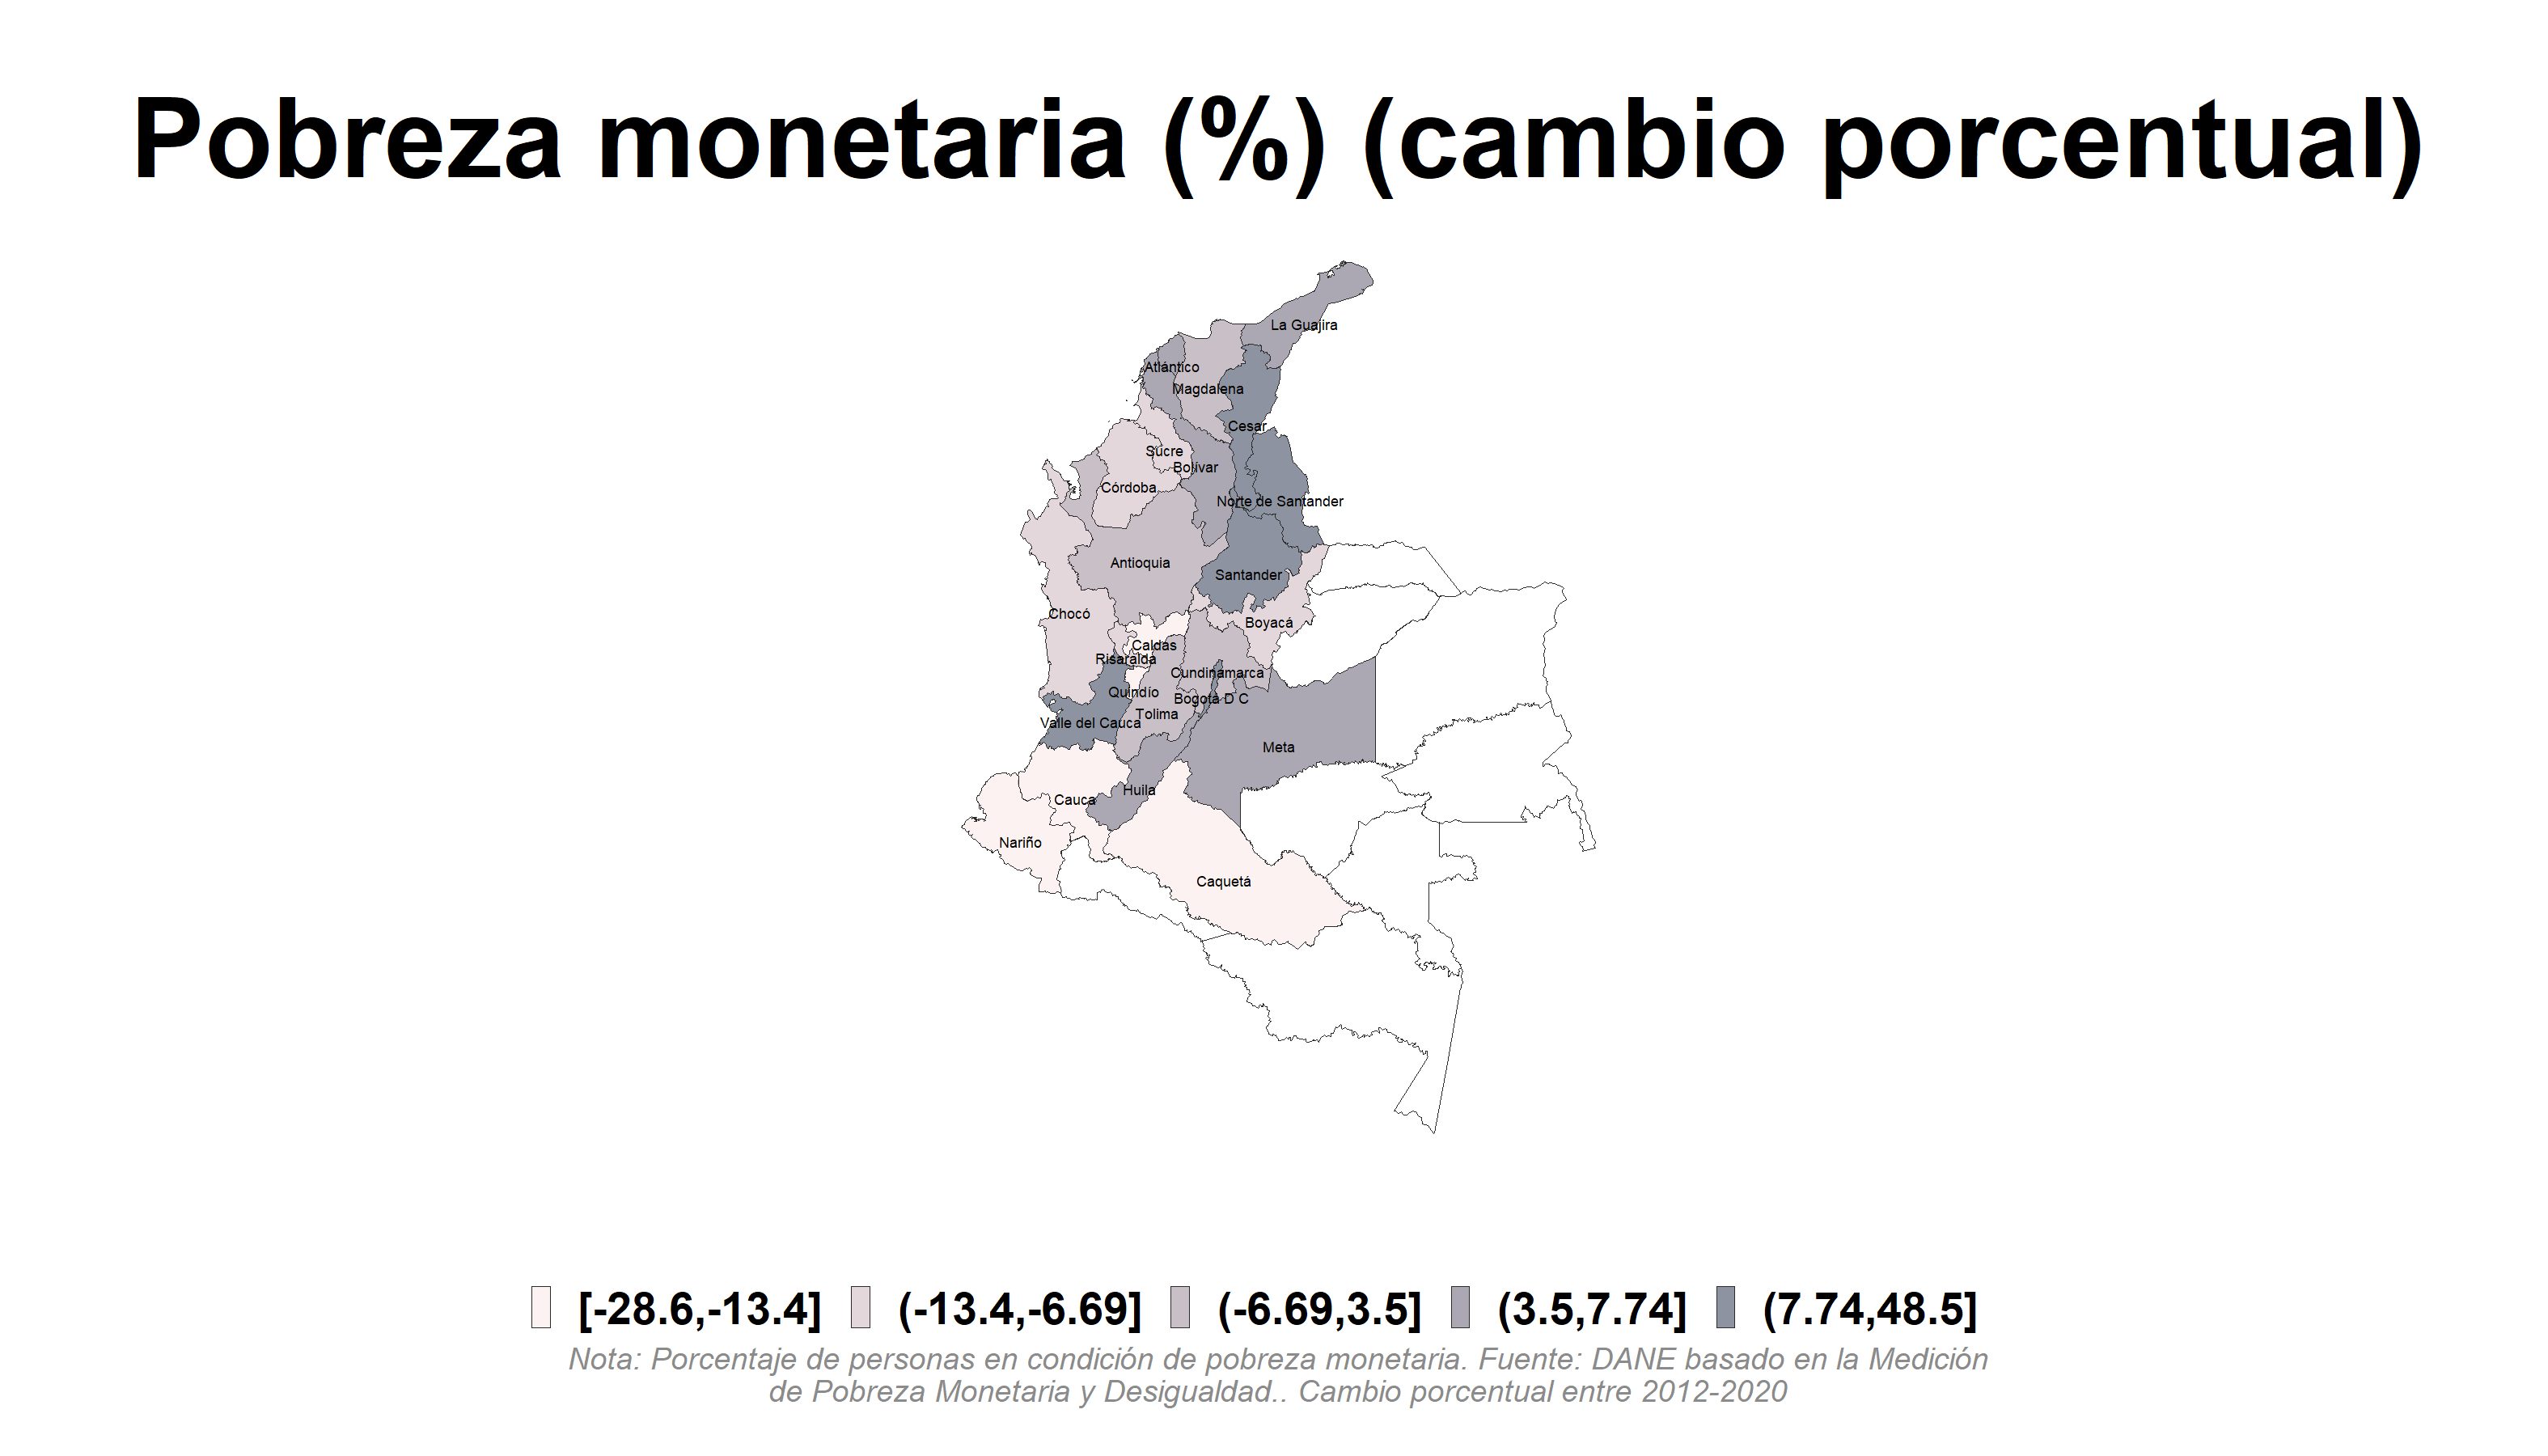
\includegraphics[width=\textwidth,keepaspectratio]{img/var_262_map_change.png}
        \end{center}
    \end{figure}
            \begin{itemize}
                    \item Cauca, Quindío, Caldas, Nariño y Caquetá son los departamentos que muestran una mayor mejoría con diferencias por encima del 13\% entre 2012 y 2020.
                    \item Los departamentos que más desmejoraron para el 2020 son Santander, Norte, Cesar y Valle, también se añade Bogotá que pasó de tener niveles por debajo del 20\% al 40\%.
                    \end{itemize}

%%%% Include figures
    \begin{figure}[H]
        \caption{Pobreza monetaria por zonas y nacional \label{map_result_2} }
        \begin{center}
        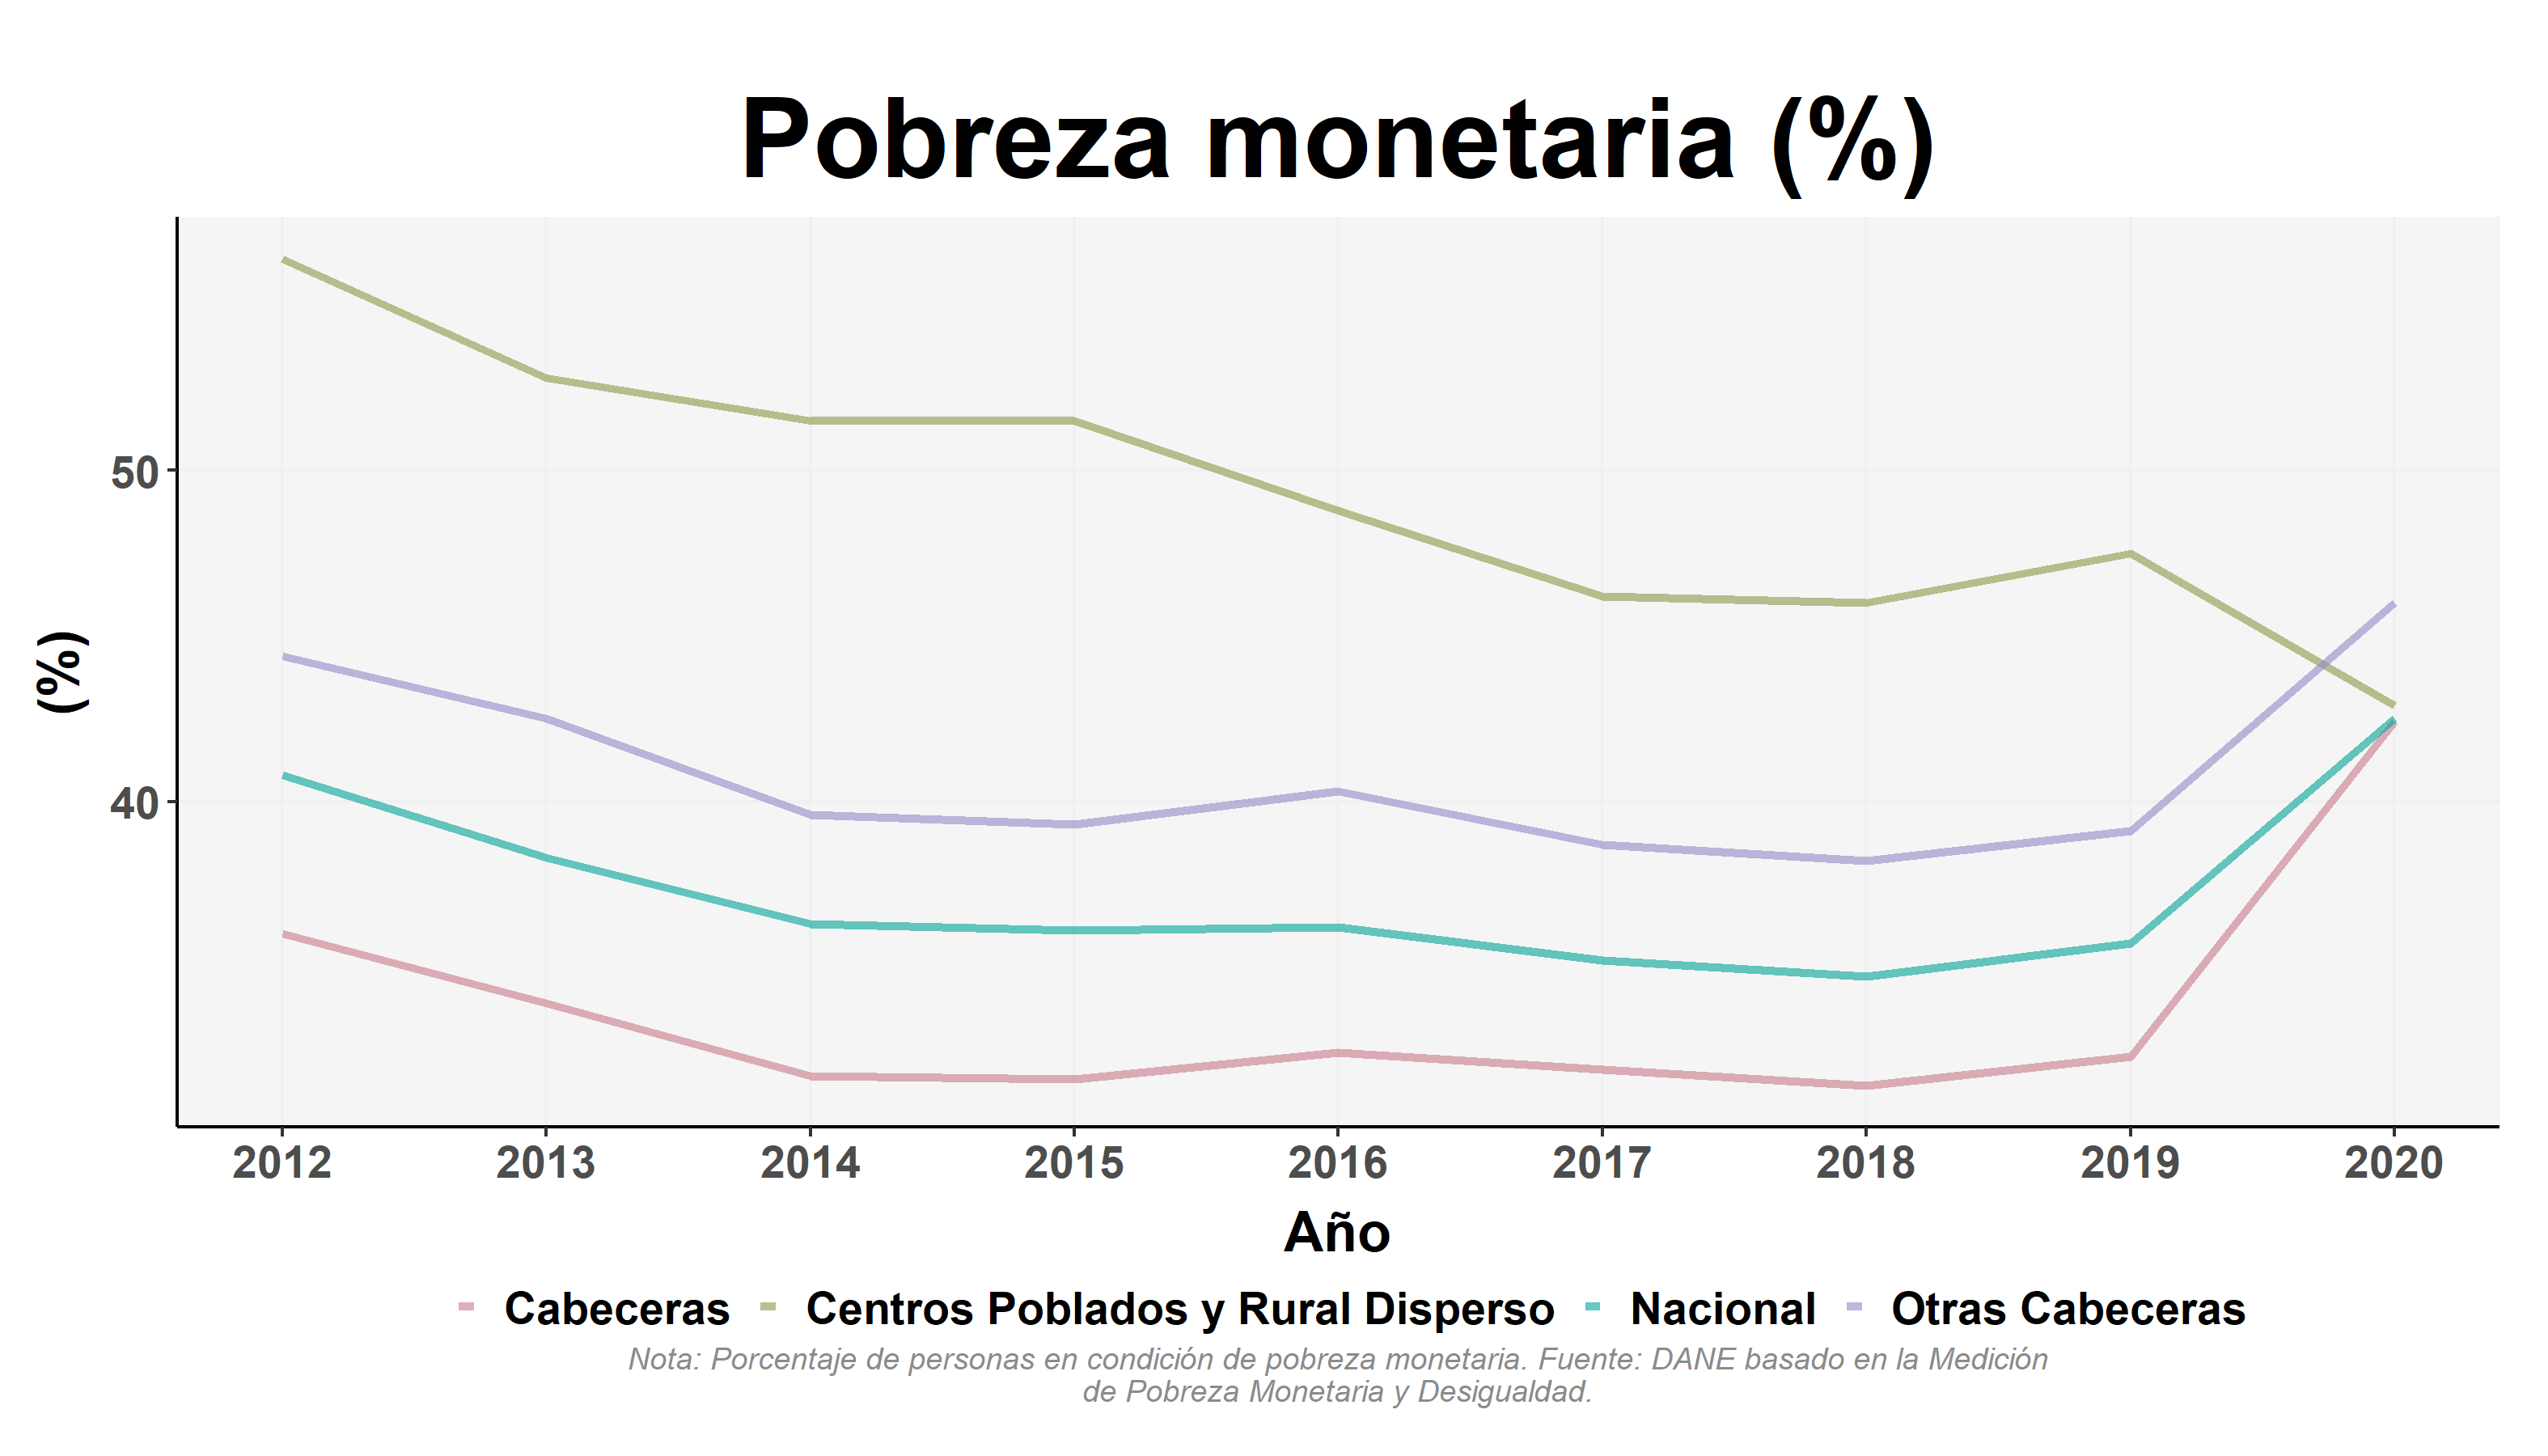
\includegraphics[width=\textwidth,keepaspectratio]{img/var_264_trend.png}
        \end{center}
    \end{figure}
            \begin{itemize}
                    \item La tendencia de los últimos 9 años muestra que la pobreza monetaria estaba descendiendo hasta el 2018, con picos en el 2016 para las cabeceras y las otras cabeceras.
                    \item La tendencia para la zona rural es la única que muestra un descenso en el 2020, el resto tienen un aumento que venía desde el 2019 y se intensifico en el 2020.
                    \item Para el 2020 el porcentaje de personas en pobreza monetaria para el nacional y las cabeceras están casi al mismo nivel que el registrado para la zona rural.
                    \item La brecha entre los valores de las cabeceras y la zona rural pasó de ser más del 15\% para el 2019 a menos del 1\% en 2020.
                    \item Las otras cabeceras sobrepasaron el porcentaje de población en pobreza monetaria registrado en 2020 para las zonas rurales y centros poblados.
                    \item Las cabeceras y a nivel nacional tienen valores similares de pobreza monetaria, 42.4\% y 42.5\% respectivamente.
                    \end{itemize}

    \subsection{Pobreza No Monetaria}

        \subsubsection{Índice de Pobreza Multidimensional - IPM}

%%%% Include figures
    \begin{figure}[H]
        \caption{Índice de Pobreza Multidimensional - Cambio porcentual entre 2018 y 2020 \label{map_result_2} }
        \begin{center}
        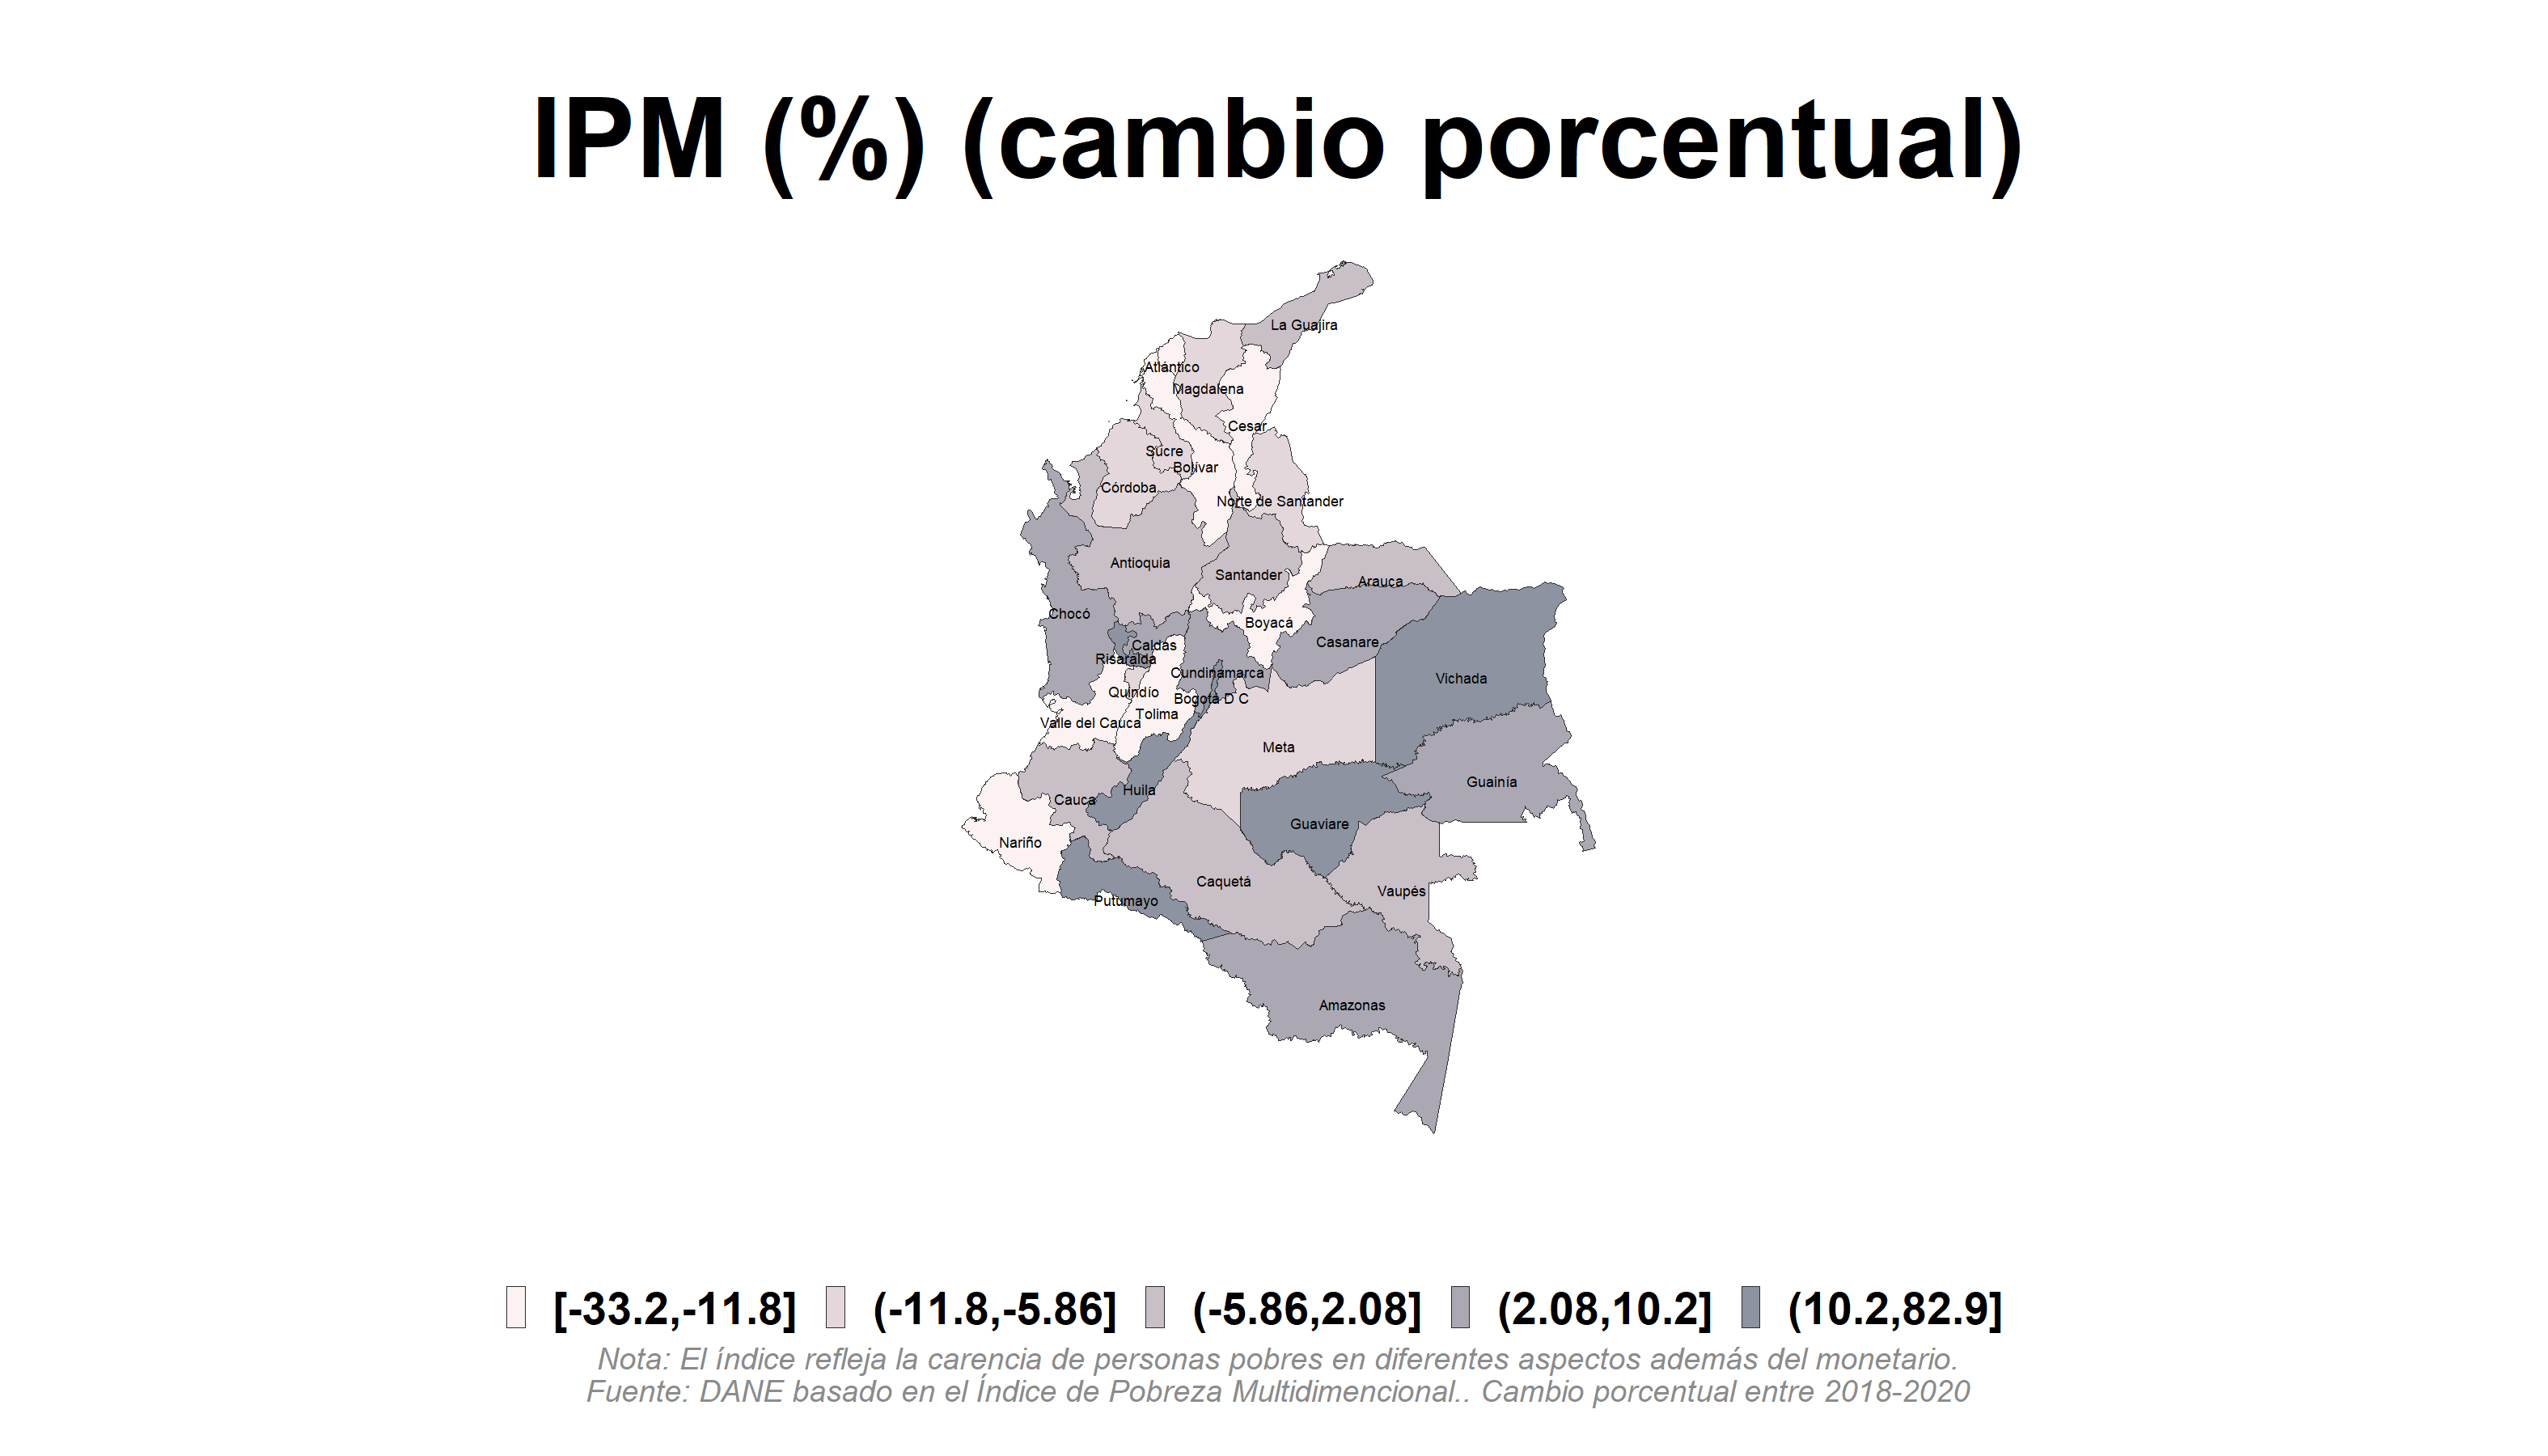
\includegraphics[width=\textwidth,keepaspectratio]{img/var_268_map_change.png}
        \end{center}
    \end{figure}
            \begin{itemize}
                    \item Nariño, Valle, Tolima, Boyacá, Bolívar, Cesar y Atlántico presentan mejoras, disminuyendo más de un 10\% su IPM entre 2018 y 2020.
                    \item Vichada, Guaviare, Putumayo, Huila, Risaralda y Bogotá aumentaron su IPM en más de un 10\% entre los años de referencia.
                    \end{itemize}

%%%% Include figures
    \begin{figure}[H]
        \caption{Índice de Pobreza Multidimensional por departamentos para el 2020 \label{map_result_2} }
        \begin{center}
        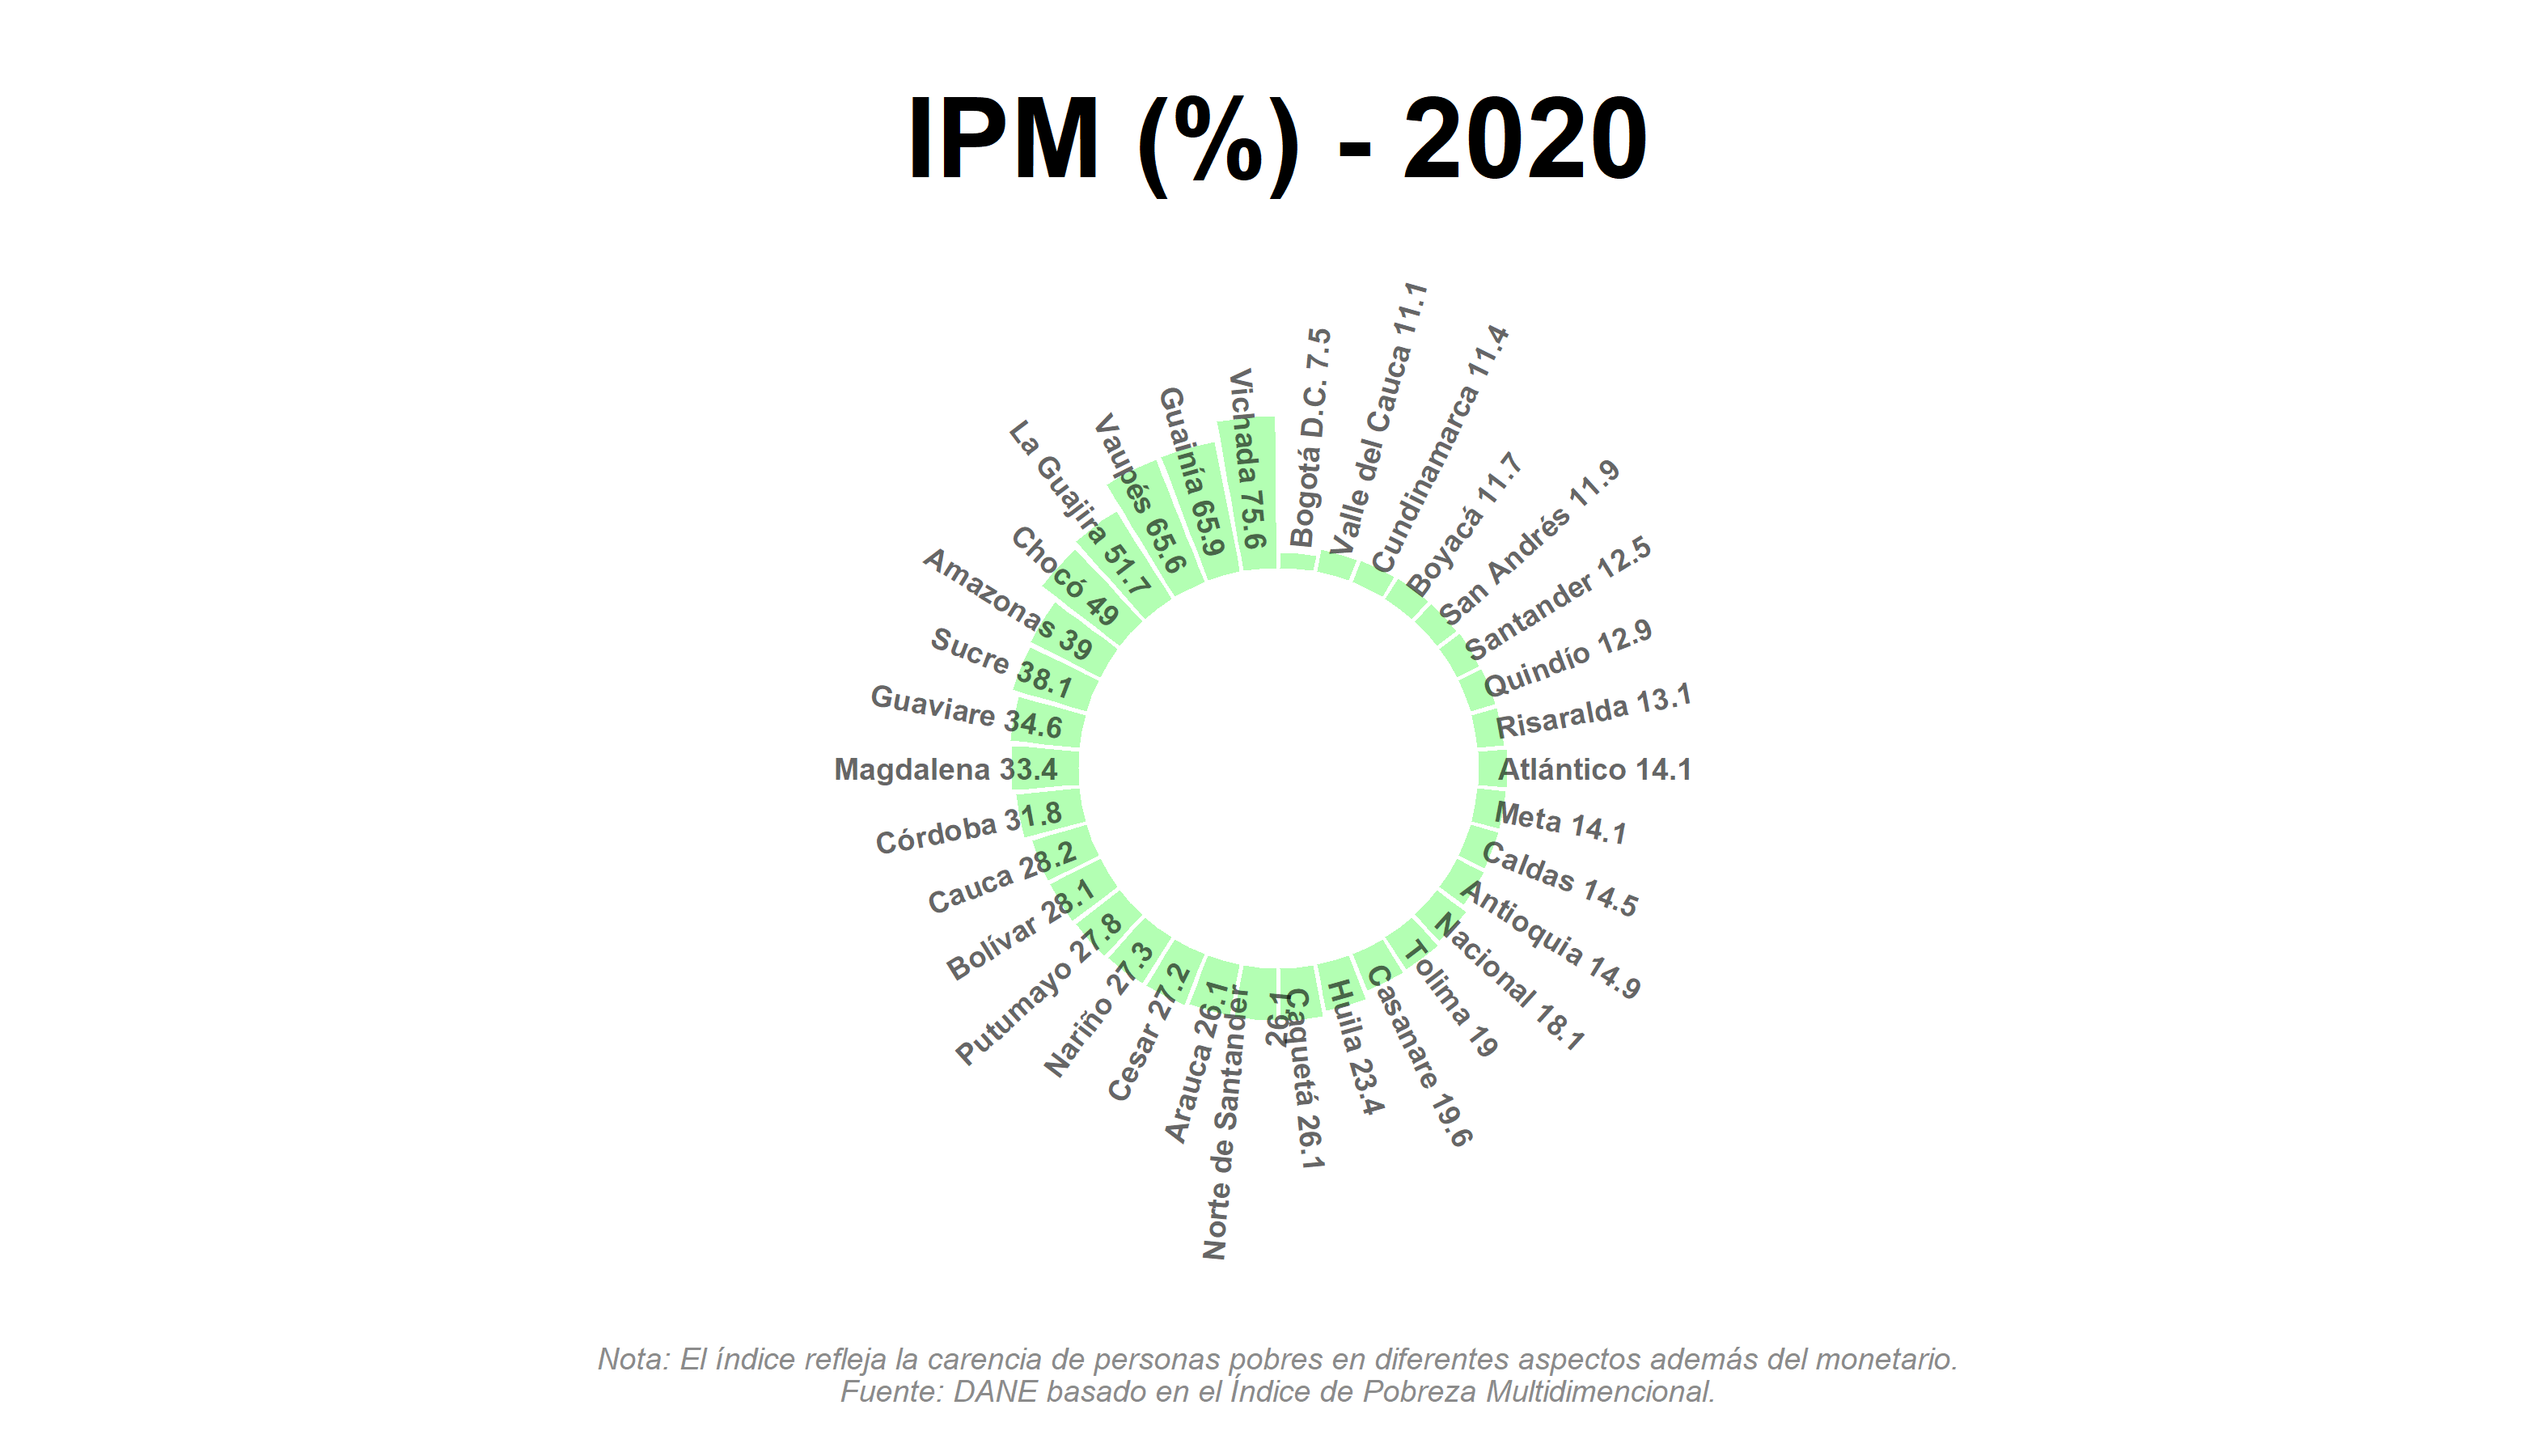
\includegraphics[width=\textwidth,keepaspectratio]{img/var_268_static.png}
        \end{center}
    \end{figure}
            \begin{itemize}
                    \item La distribución del IPM es amplia, desde menos del 10\% hasta por encima del 75\%.
                    \item La diferencia entre los dptos extremos es de aproximadamente un 65\%, teniendo a Bogotá (Distrito capital) con el de menor (7.5\%) y Vichada el de mayor puntaje con un 75.6\%.  
                    \item Hay una diferencia de aproximadamente un 15\% entre los últimos 3 departamentos y el anterior a este, siendo el salto más abrupto en el IPM
                    \end{itemize}

%%%% Include figures
    \begin{figure}[H]
        \caption{Índice de Pobreza Multidimensional por regiones - 2010 VS 2020 \label{map_result_2} }
        \begin{center}
        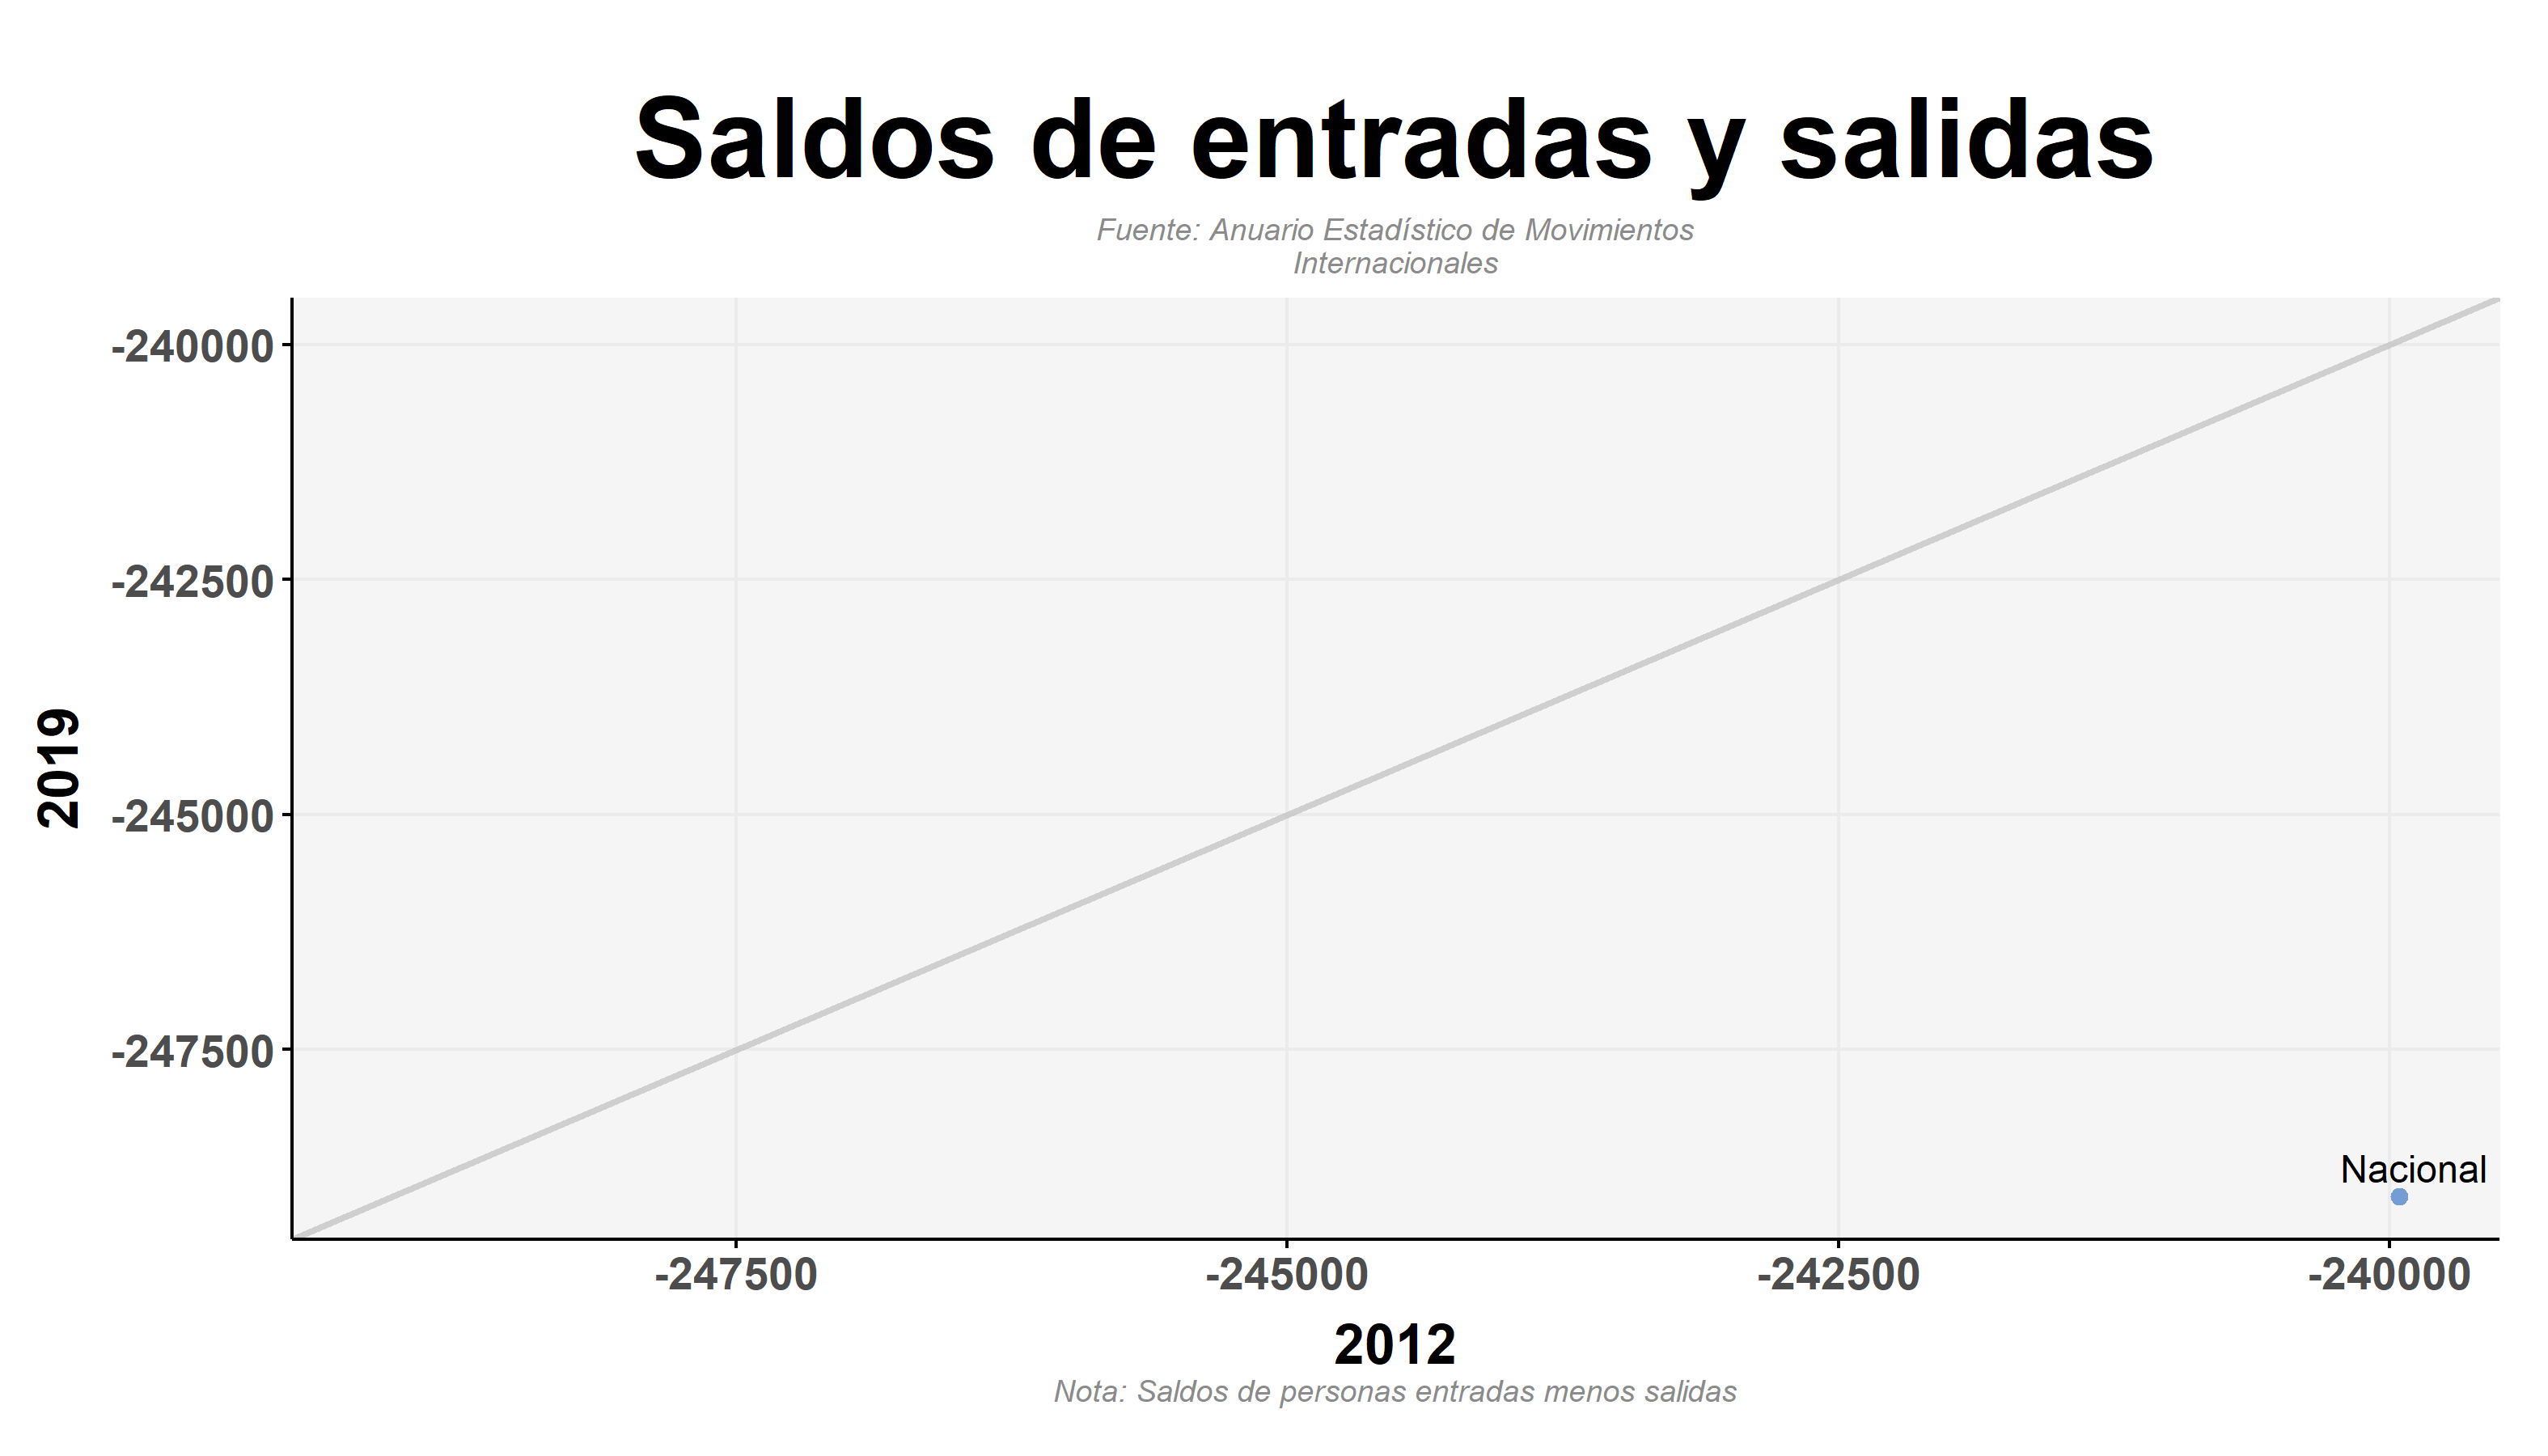
\includegraphics[width=\textwidth,keepaspectratio]{img/var_270_scatter_time.png}
        \end{center}
    \end{figure}
            \begin{itemize}
                    \item Todas las regiones tuvieron resultados menores en para 2020 comparados con los del 2012.
                    \item La distribución de puestos no cambio a excepción de los dos primeros (IPM más altos) donde la región Pacífica pasó de ser segundo a reemplazar a la Caribe que estaba de primero en el 2012.
                    \item La región Caribe es la que presenta una mayor mejoría, aproximadamente un 15\%.
                    \end{itemize}

%%%% Include figures
    \begin{figure}[H]
        \caption{Índice de Pobreza Multidimensional por zonas y nacional \label{map_result_2} }
        \begin{center}
        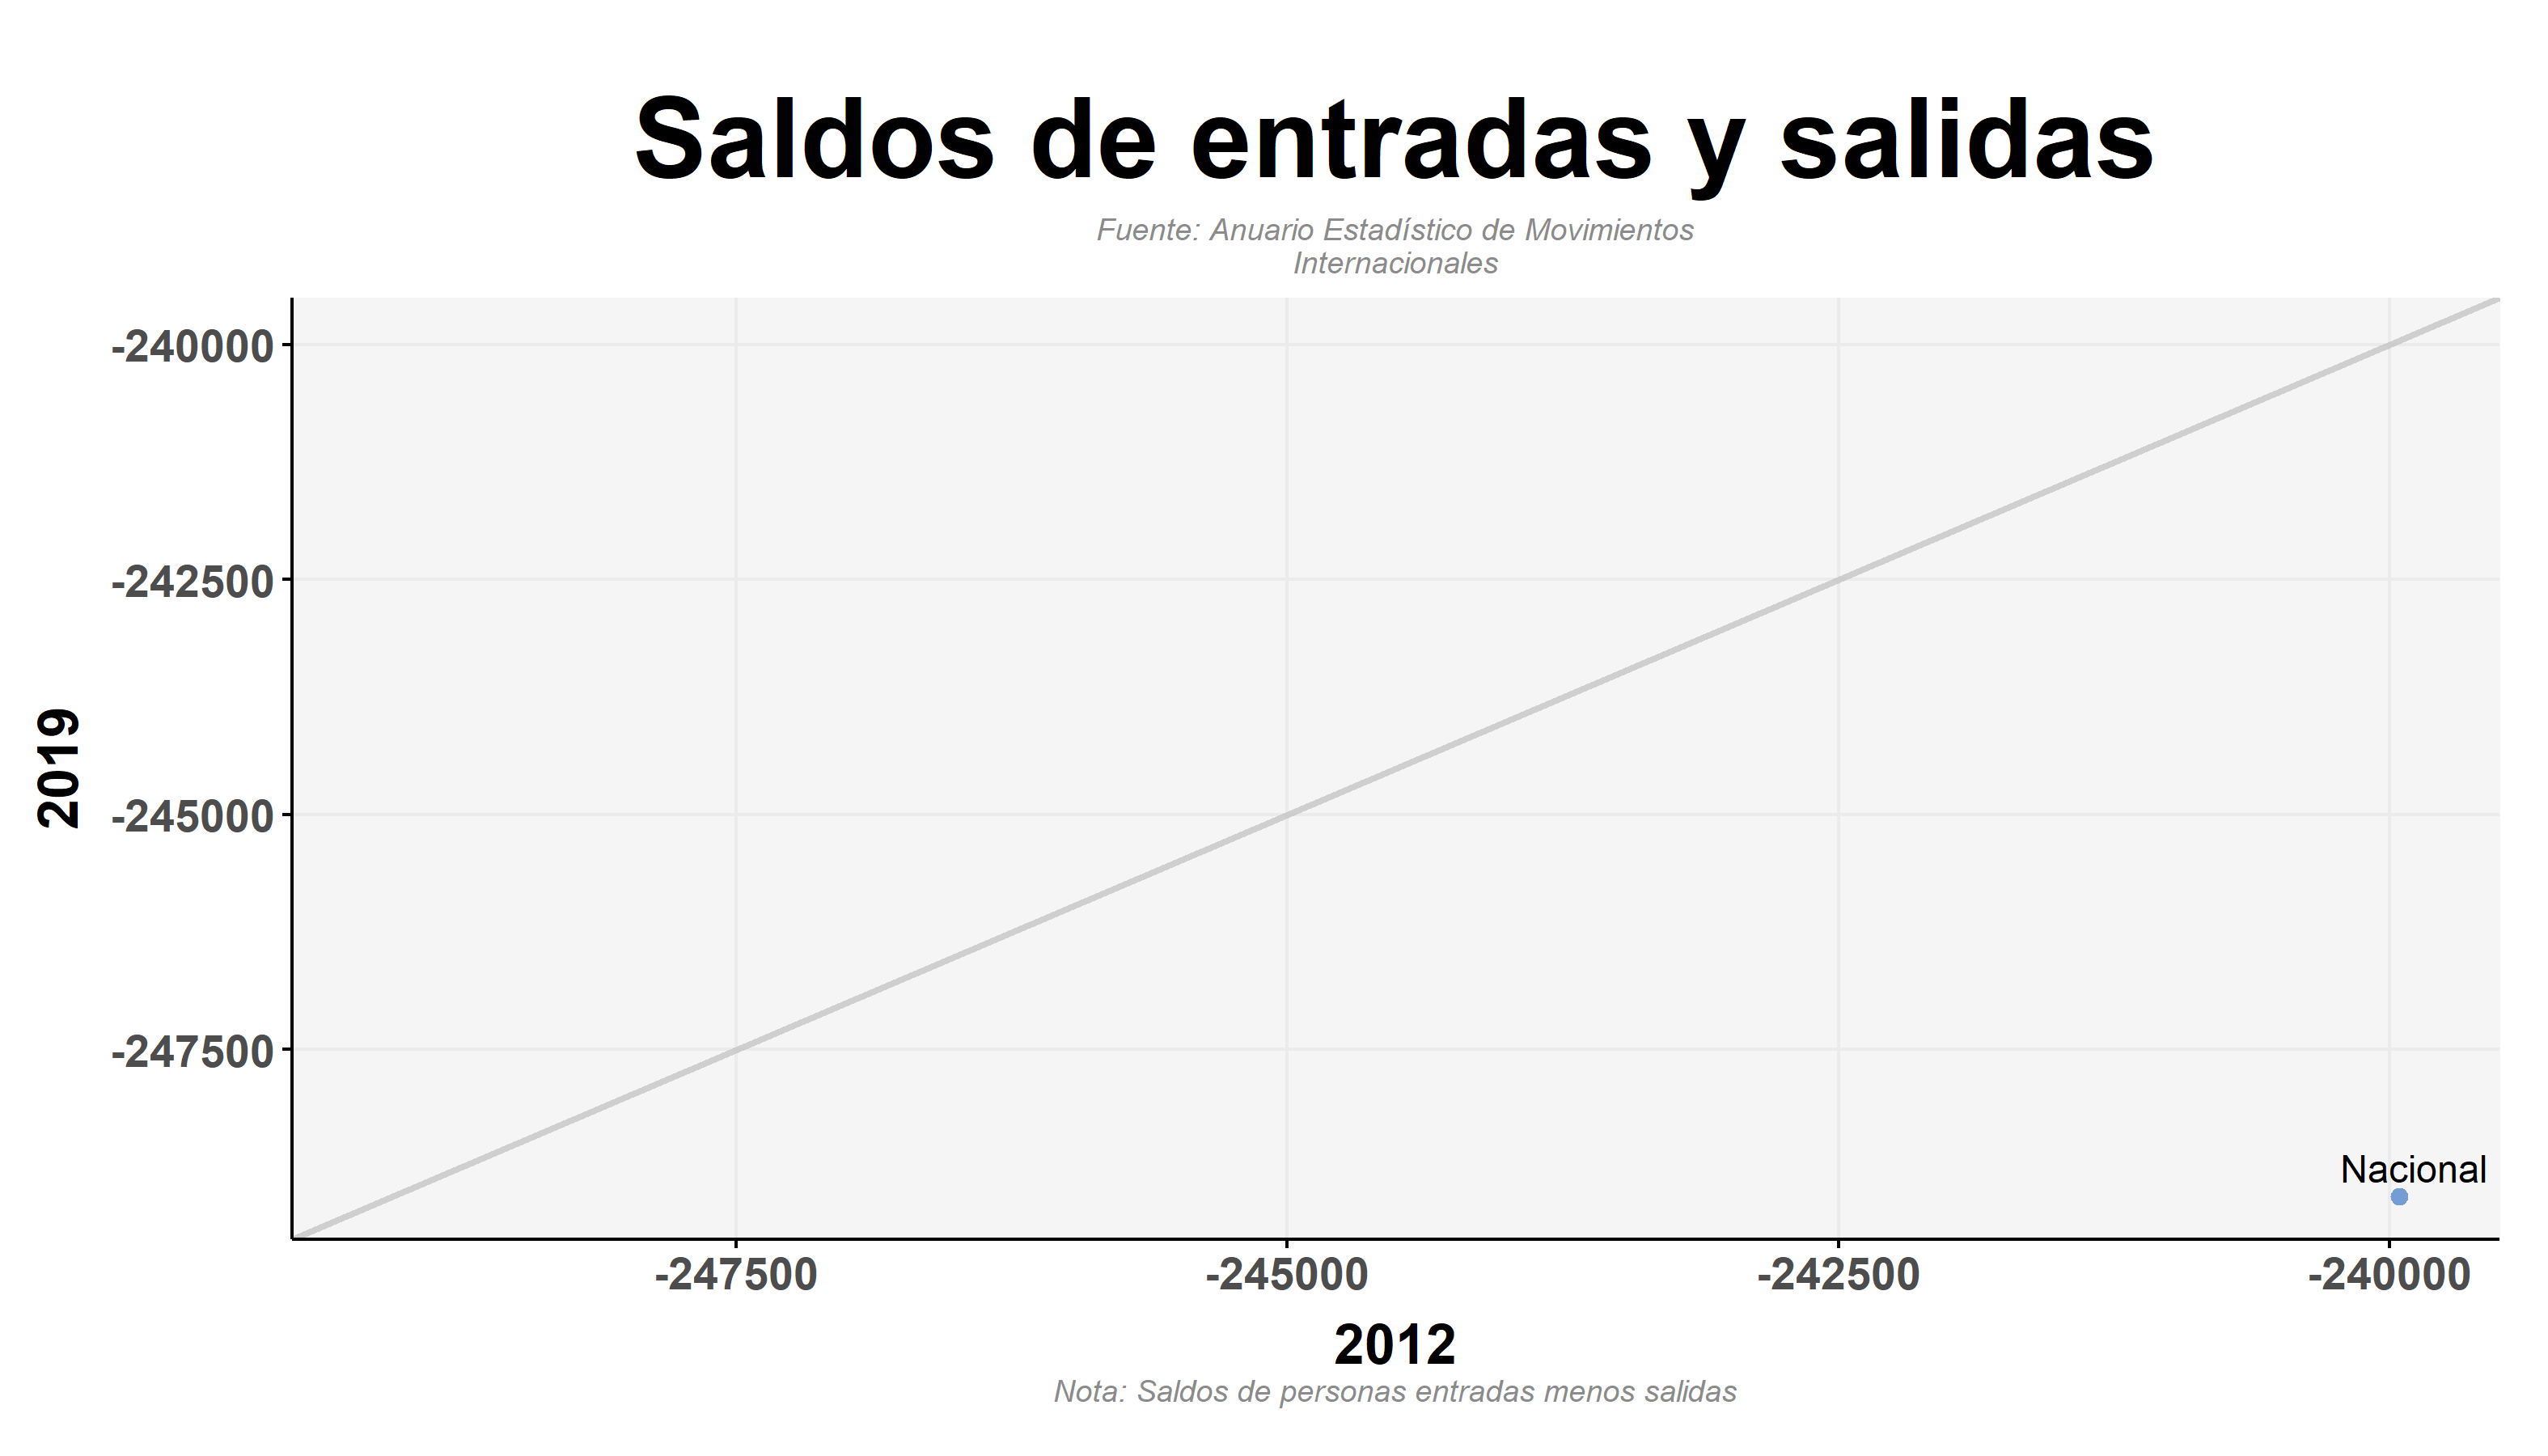
\includegraphics[width=\textwidth,keepaspectratio]{img/var_270_scatter_time.png}
        \end{center}
    \end{figure}
            \begin{itemize}
                    \item El IPM en general vemos que para las cabeceras y nacional han estado bajando y desde el 2017 se han subido los niveles levemente hasta el pico en el 2018, donde baja para 2019 y hay un leve aumento en 2020.
                    \item A nivel de centros poblados y rural vemos que a pesar de tener el mismo comportamiento sus cambios son más abruptos, como el pico de 2018 que se denota que viene aumentando después del 2016 y el del 2020 que aparece como un retroceso de la mitad de lo que disminuyó en 2019.
                    \item Para el 2020 se registraron IPM menores que los registrados en 2010, lo que demuestra una mejora en los últimos 10 años.
                    \item La zona rural parece más sensible a los cambios en términos del IPM.
                    \end{itemize}

        \subsubsection{Necesidades Básicas Insatisfechas - NBI}
        
%%%% Include figures
    \begin{figure}[H]
        \caption{Necesidades Básicas Insatisfechas - Minorías VS no minorías \label{map_result_2} }
        \begin{center}
        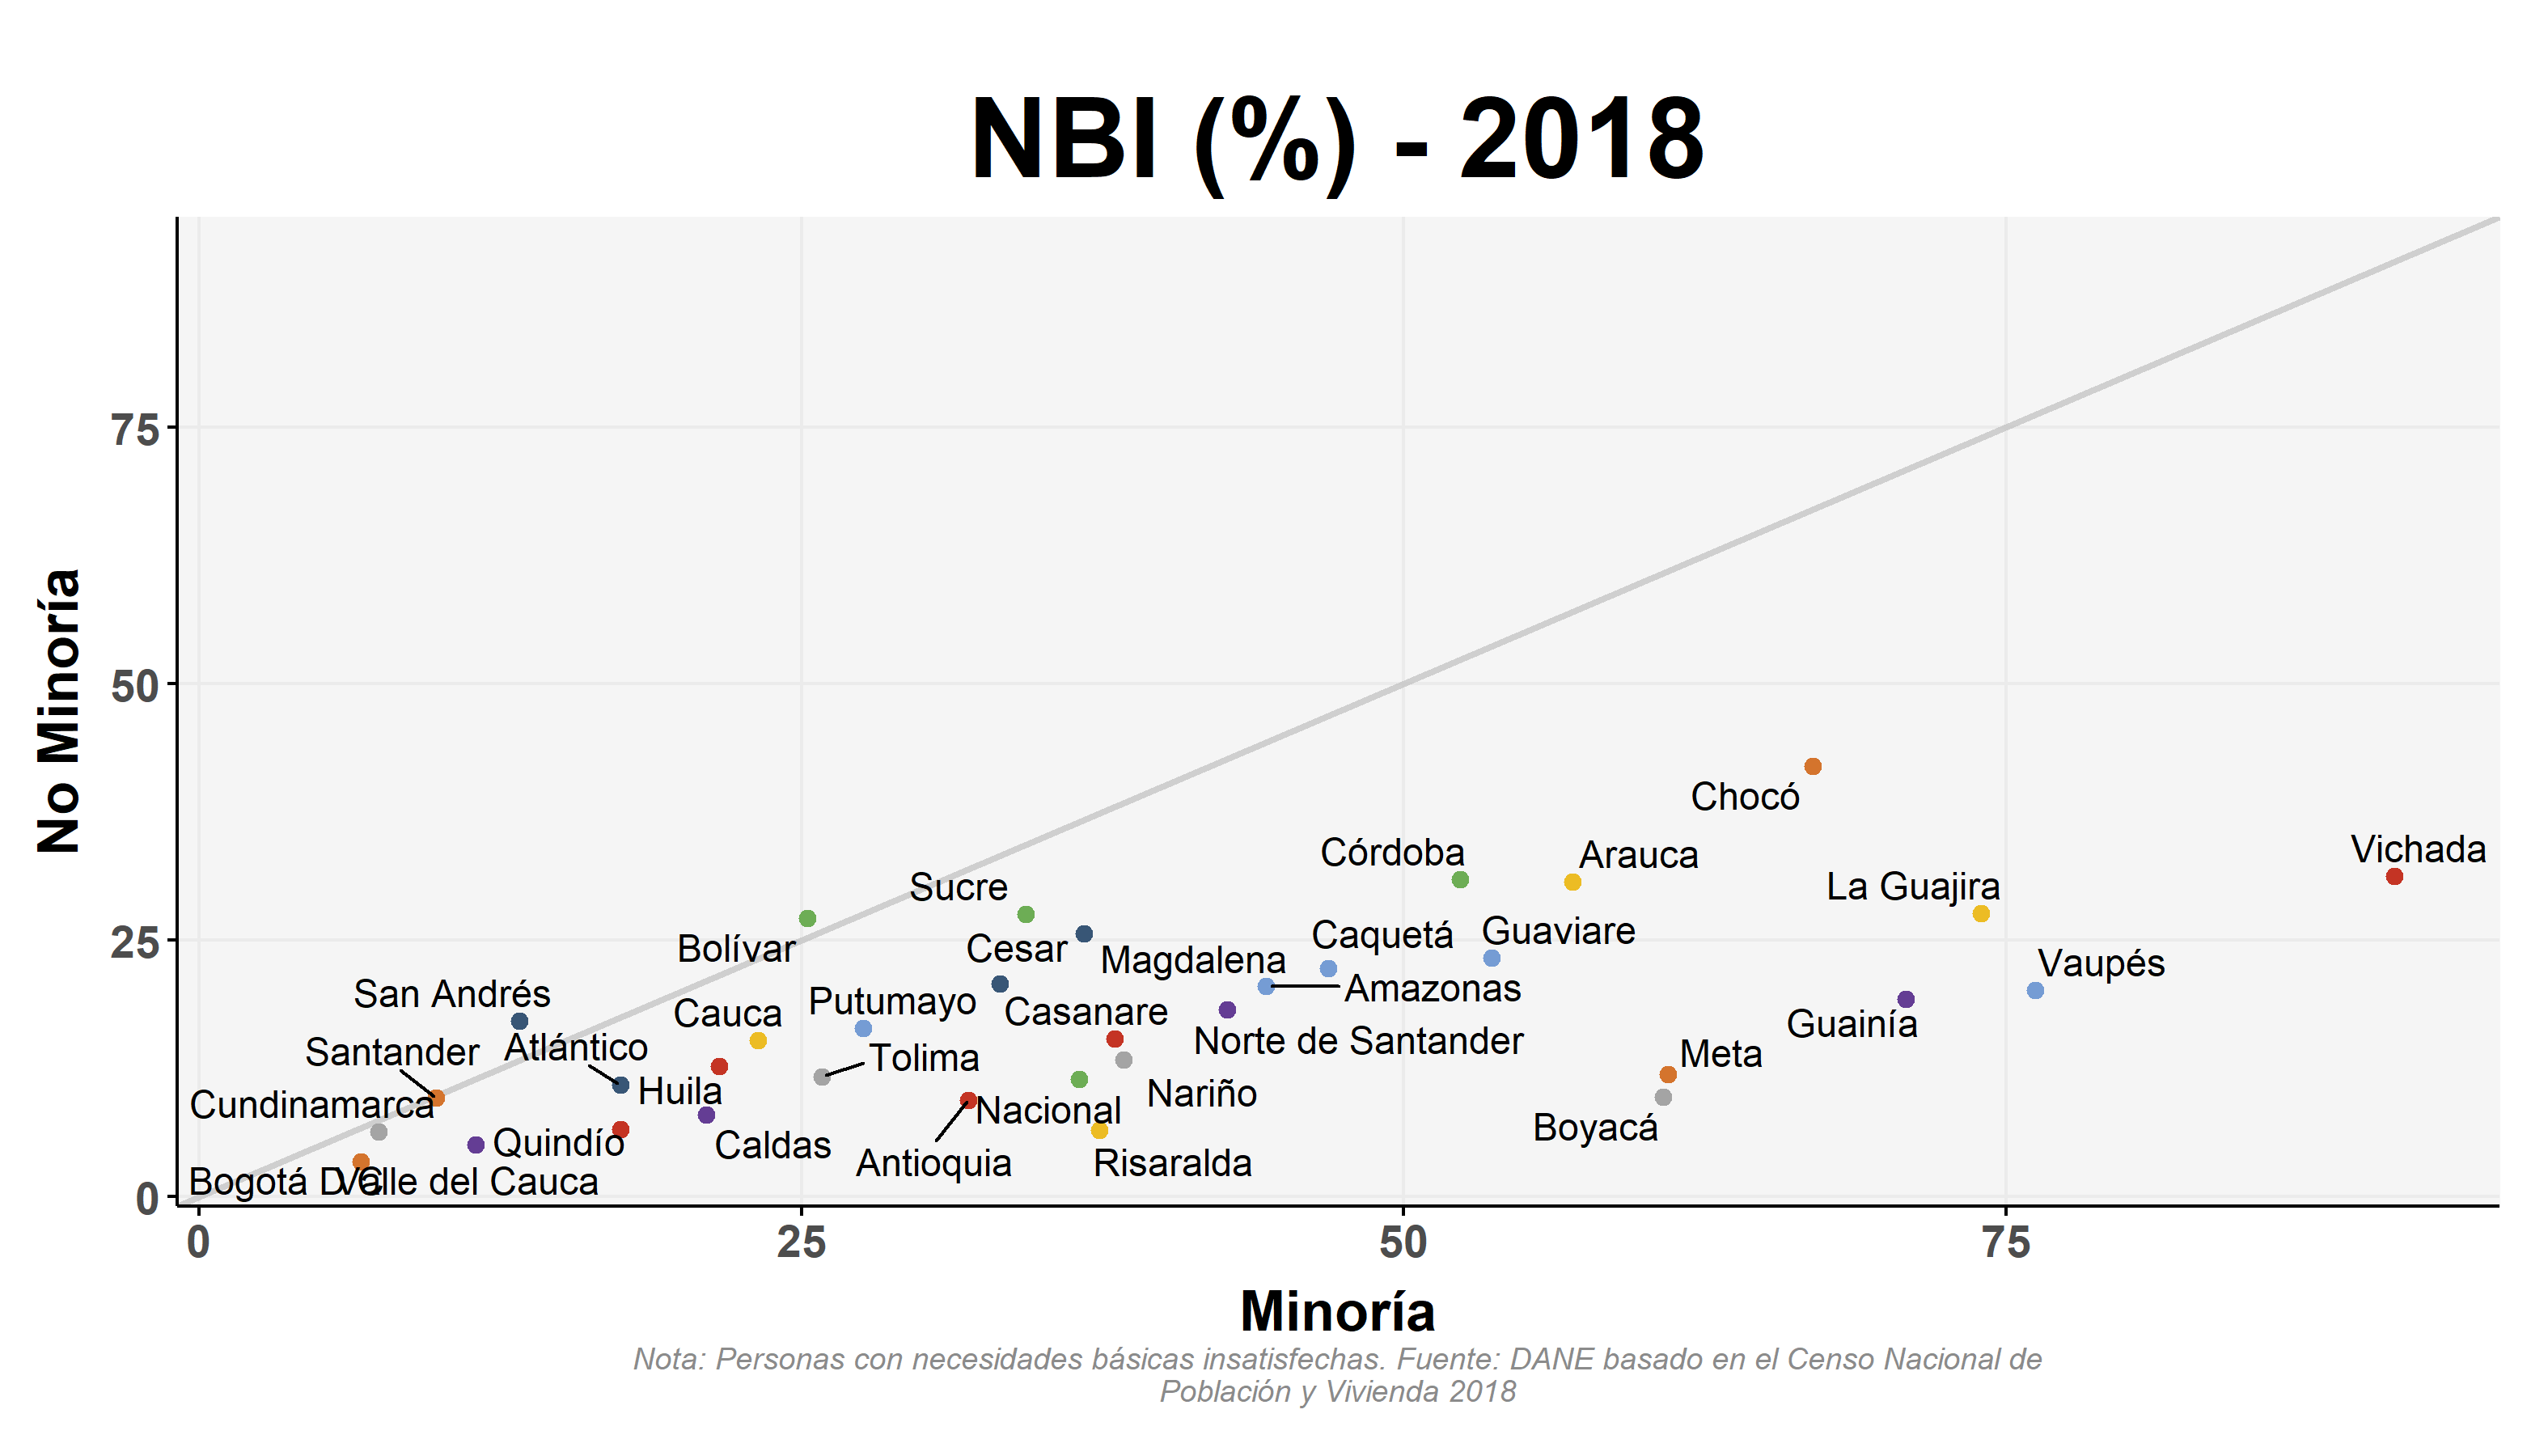
\includegraphics[width=\textwidth,keepaspectratio]{img/var_272_scatter.png}
        \end{center}
    \end{figure}
            \begin{itemize}
                    \item Gran parte de los departamentos tienen NBI de las no minorías por debajo del 30\%, mientras que las de las minorías están distribuidas entre 0 y 75\%. 
                    \item Solo San Andrés y Bolívar presentan NBI mayores para las no minorías que para las minorías.
                    \item Cundinamarca y Santander presentan valores similares de NBI entre minorías y no minorías.
                    \item A nivel nacional encontramos que las minorías tienen NBI por encima del 35\% mientras que las no minorías están cerca del 10\%, con una diferencias de más del 20\%.
                    \end{itemize}

%%%% Include figures
    \begin{figure}[H]
        \caption{Necesidades Básicas Insatisfechas para minorías y no minorías en el 2018 \label{map_result_2} }
        \begin{center}
        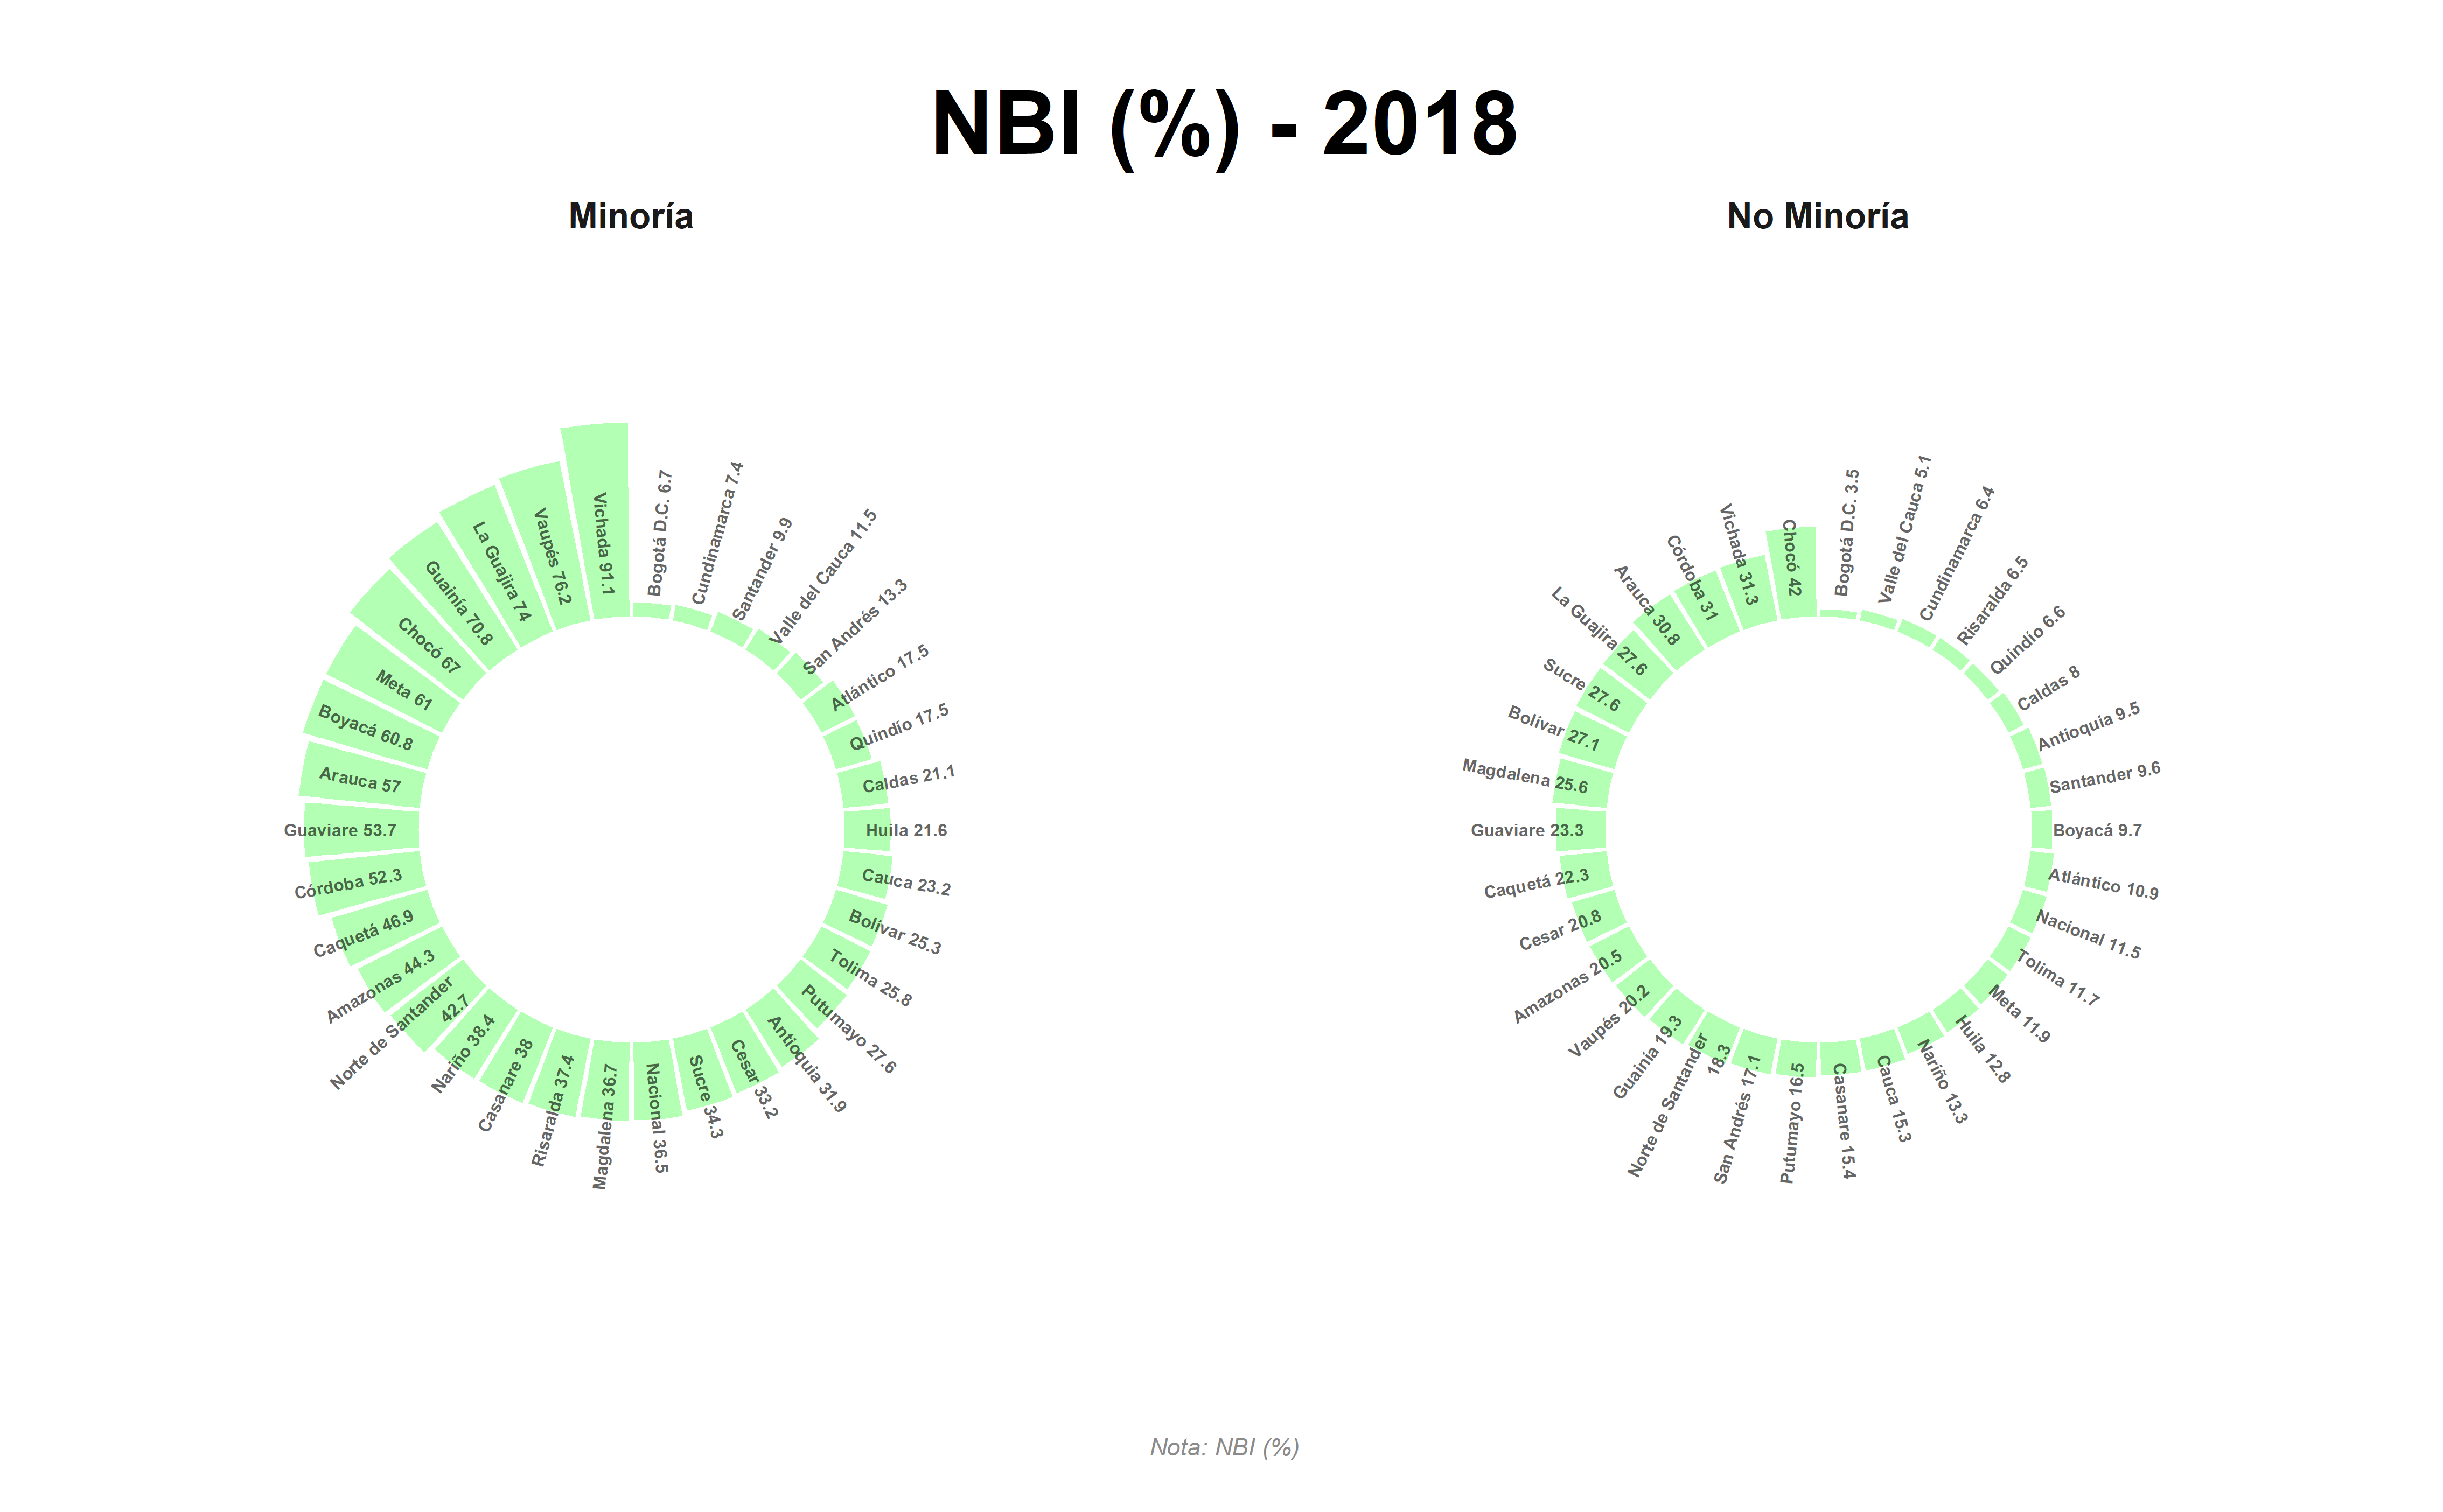
\includegraphics[width=\textwidth,keepaspectratio]{img/var_272_static.png}
        \end{center}
    \end{figure}
            \begin{itemize}
                    \item Bogotá es la zona con menor nivel de NBI para ambos, mientras que Vichada es el de mayor para las minorías y Chocó para las no minorías.
                    \item La diferencia entre las zonas extremos es de poco menos del 40\% para las no minorías (Bogotá - Chocó) y de más del 80\% para las minorías (Bogotá - Vichada).
                    \item La distribución de NBI es menor para las no minorías (3 a 42\%), teniendo un salto del 10\% aproximadamente entre el último y el anterior a este, mientras que las minorías tienen una mayor área de distribución (6 a 92\%) con un salto de aproximadamente 15\% entre los dos últimos.
                    \end{itemize}

%%%% Include figures
    \begin{figure}[H]
        \caption{Necesidades Básicas Insatisfechas por departamentos para el 2018 \label{map_result_2} }
        \begin{center}
        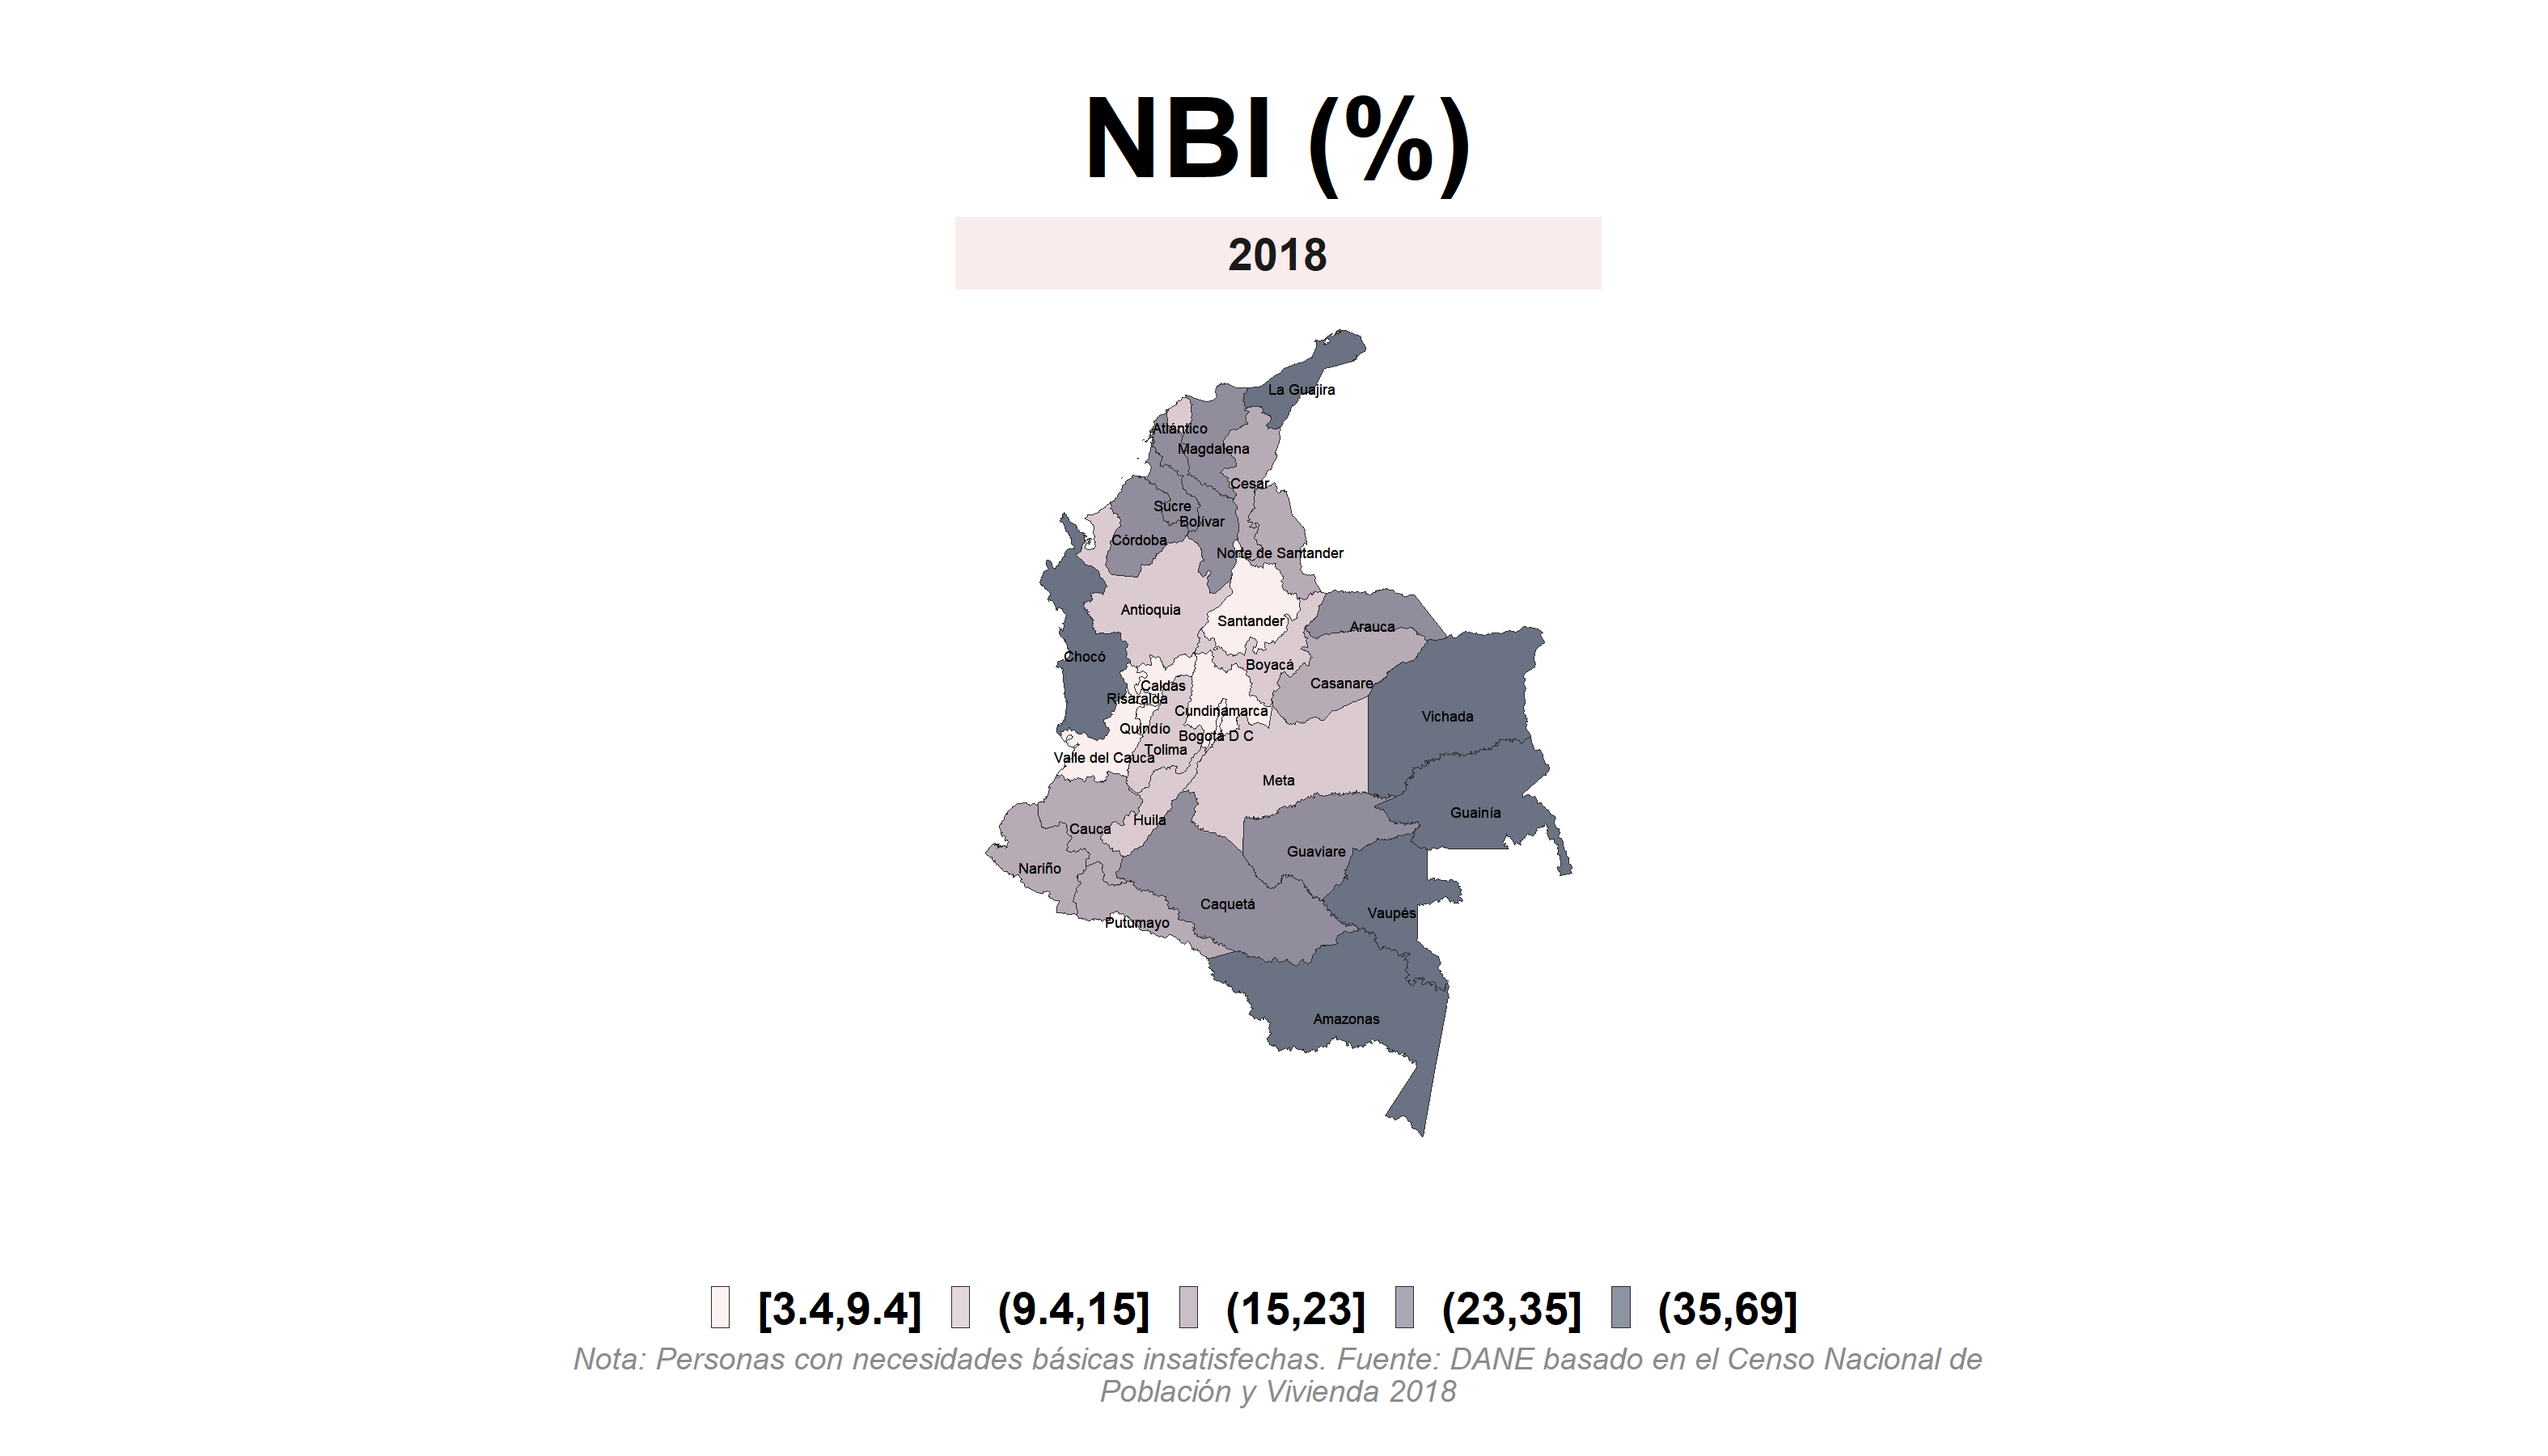
\includegraphics[width=\textwidth,keepaspectratio]{img/var_273_map.png}
        \end{center}
    \end{figure}
            \begin{itemize}
                    \item Valle, Quindío, Risaralda, Caldas, Cundinamarca, Bogotá y Santander son los departamentos con menor porcentaje de NBI, menos del 10\%.
                    \item Se ve que hacia el centro del país se encuentran los departamentos con menores niveles de NBI, mientras que a la periferia se ve como aumentan estas.
                    \item Vichada, Guainía, Vaupés, Amazonas, Chocó y La Guajira tienen el mayor porcentaje de NBI, por encima de 35\%. Todos los departamentos están en la frontera del país, siendo gran parte de estos en los llanos orientales y la Amazonia.
                    \end{itemize}

%%%% Include figures
    \begin{figure}[H]
        \caption{Necesidades Básicas Insatisfechas por departamentos para 2018 \label{map_result_2} }
        \begin{center}
        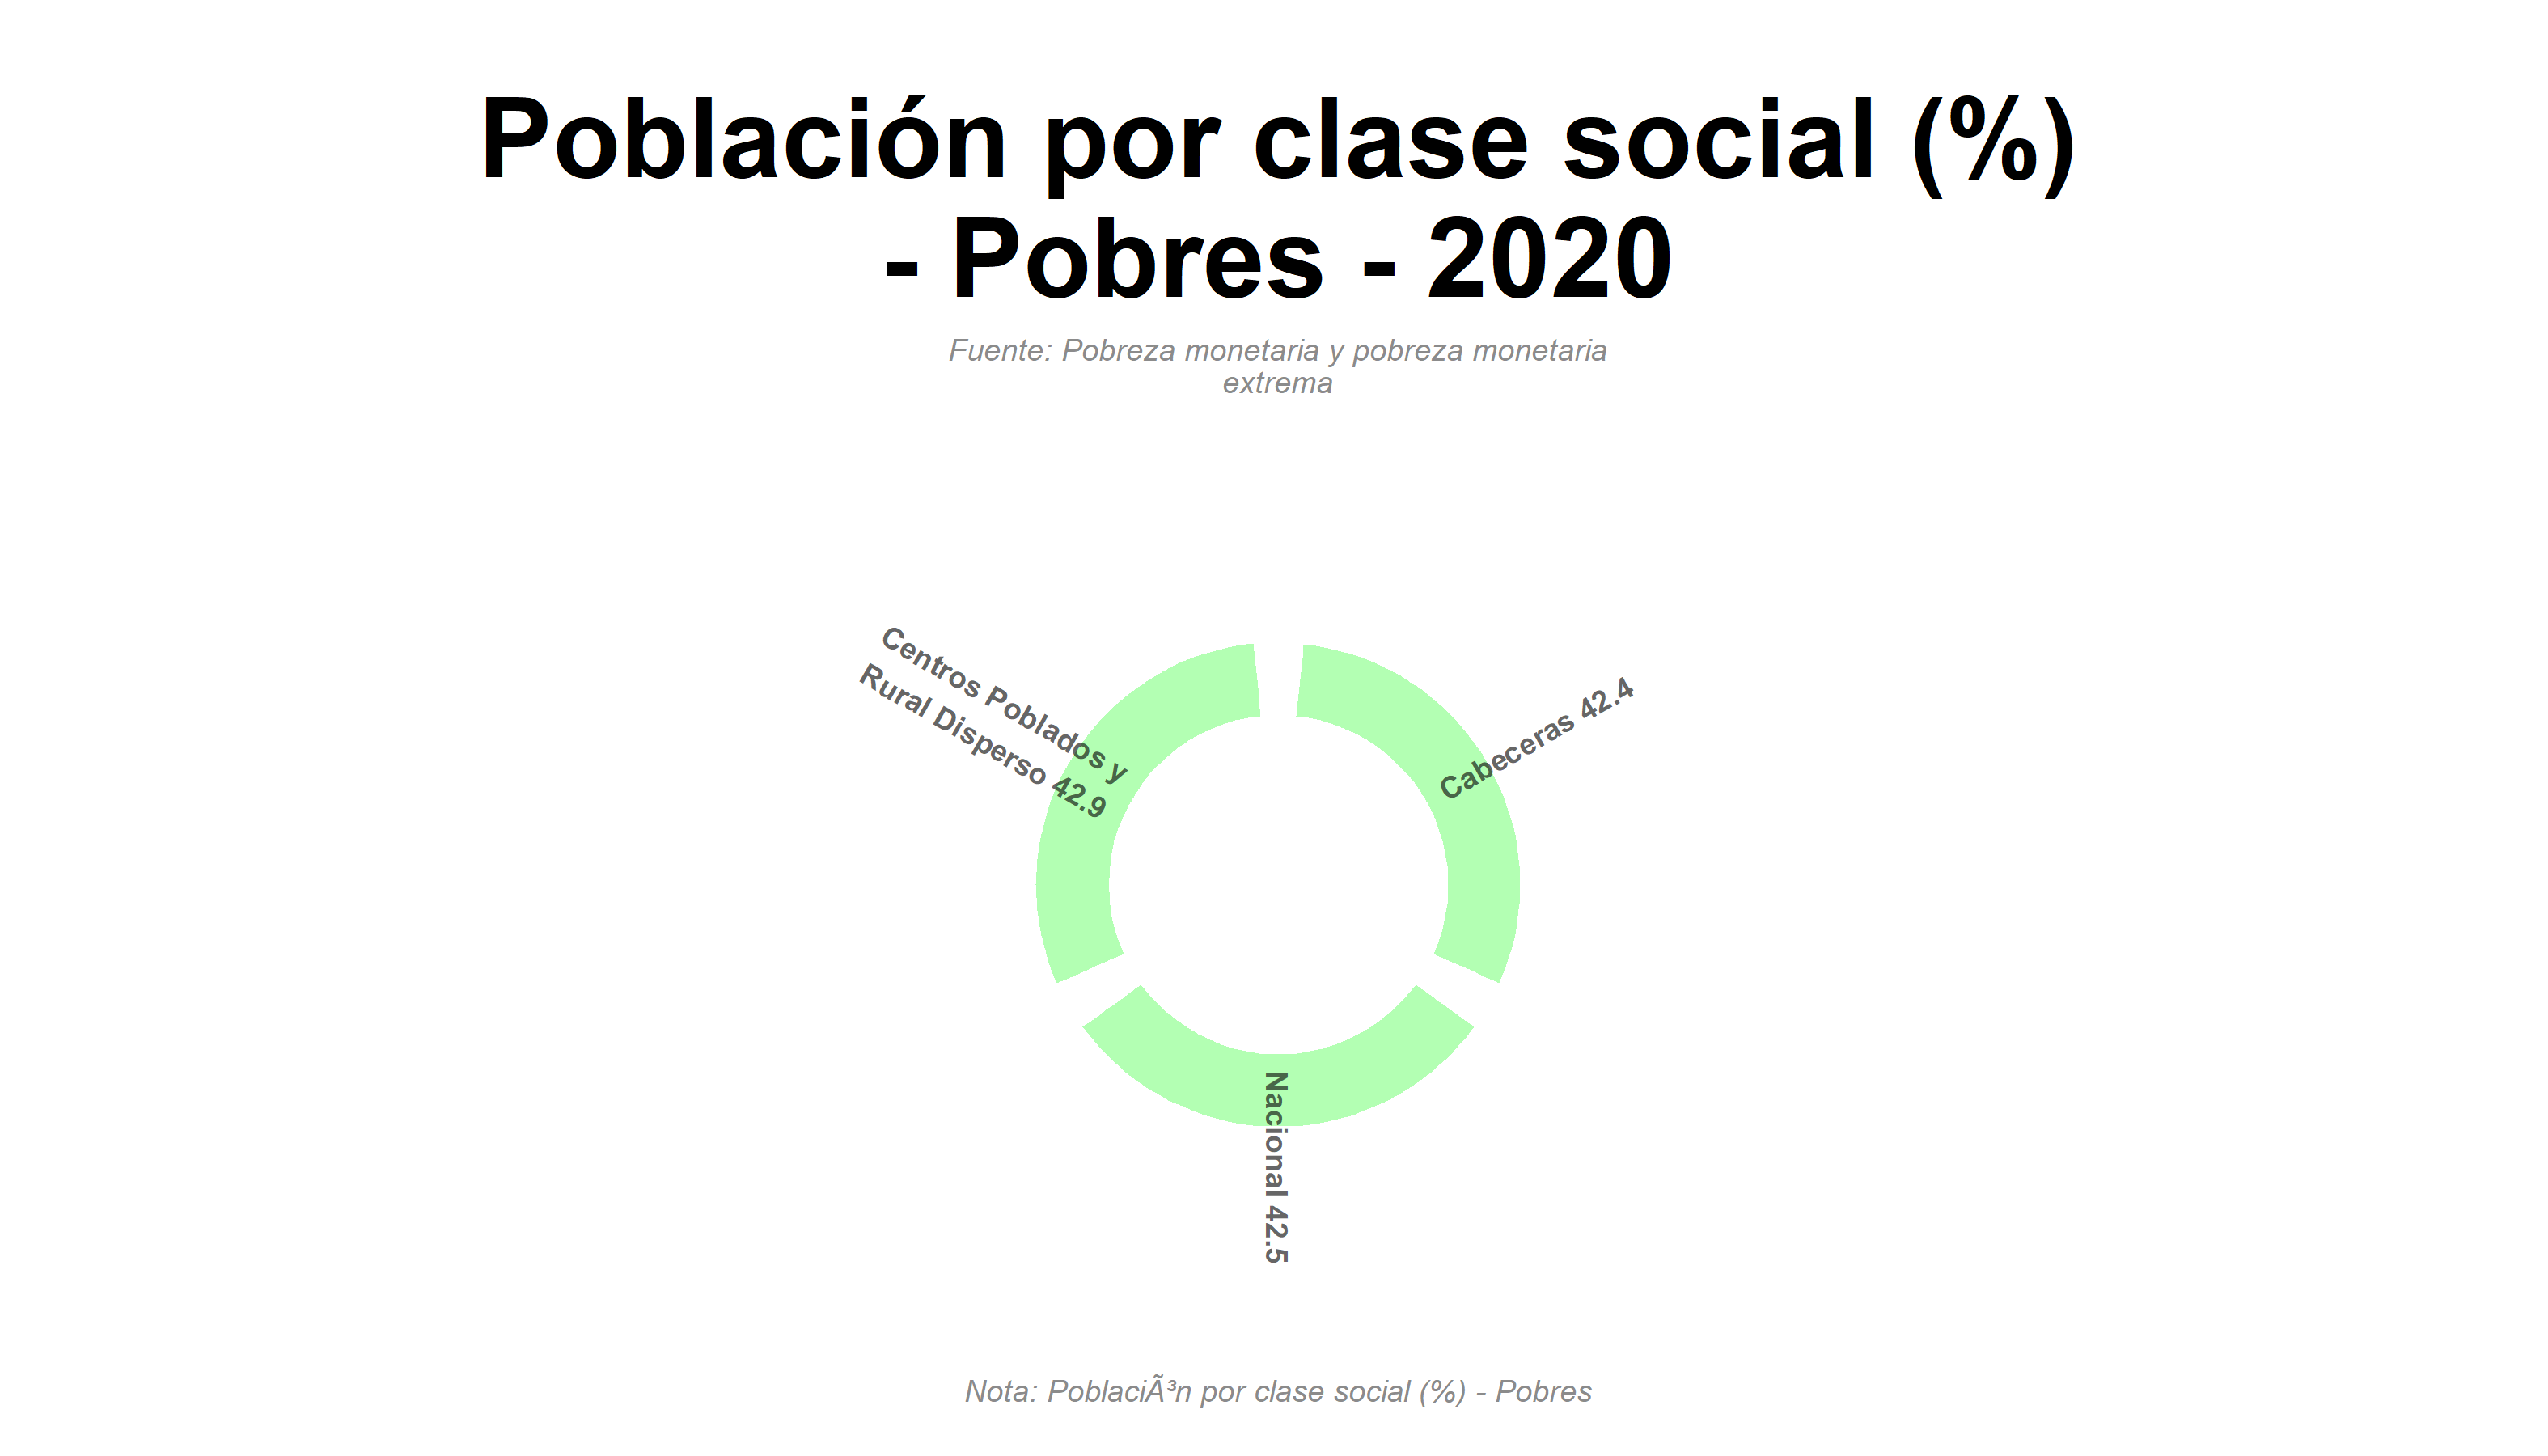
\includegraphics[width=\textwidth,keepaspectratio]{img/var_273_static.png}
        \end{center}
    \end{figure}
            \begin{itemize}
                    \item La distribución de las NBI está en gran parte de los dptos entre 3 y 35\%, y los últimos 5 dptos entre 50 y 69\%, siendo un salto de poco más del 15\% entre estos y el anterior a estos.
                    \item La diferencia entre las zonas extremo es de aproximadamente un 65\% (Bogotá - Vaupés)
                    \end{itemize}

%%%% Include figures
    \begin{figure}[H]
        \caption{Necesidades Básicas Insatisfechas por zonas y nacional \label{map_result_2} }
        \begin{center}
        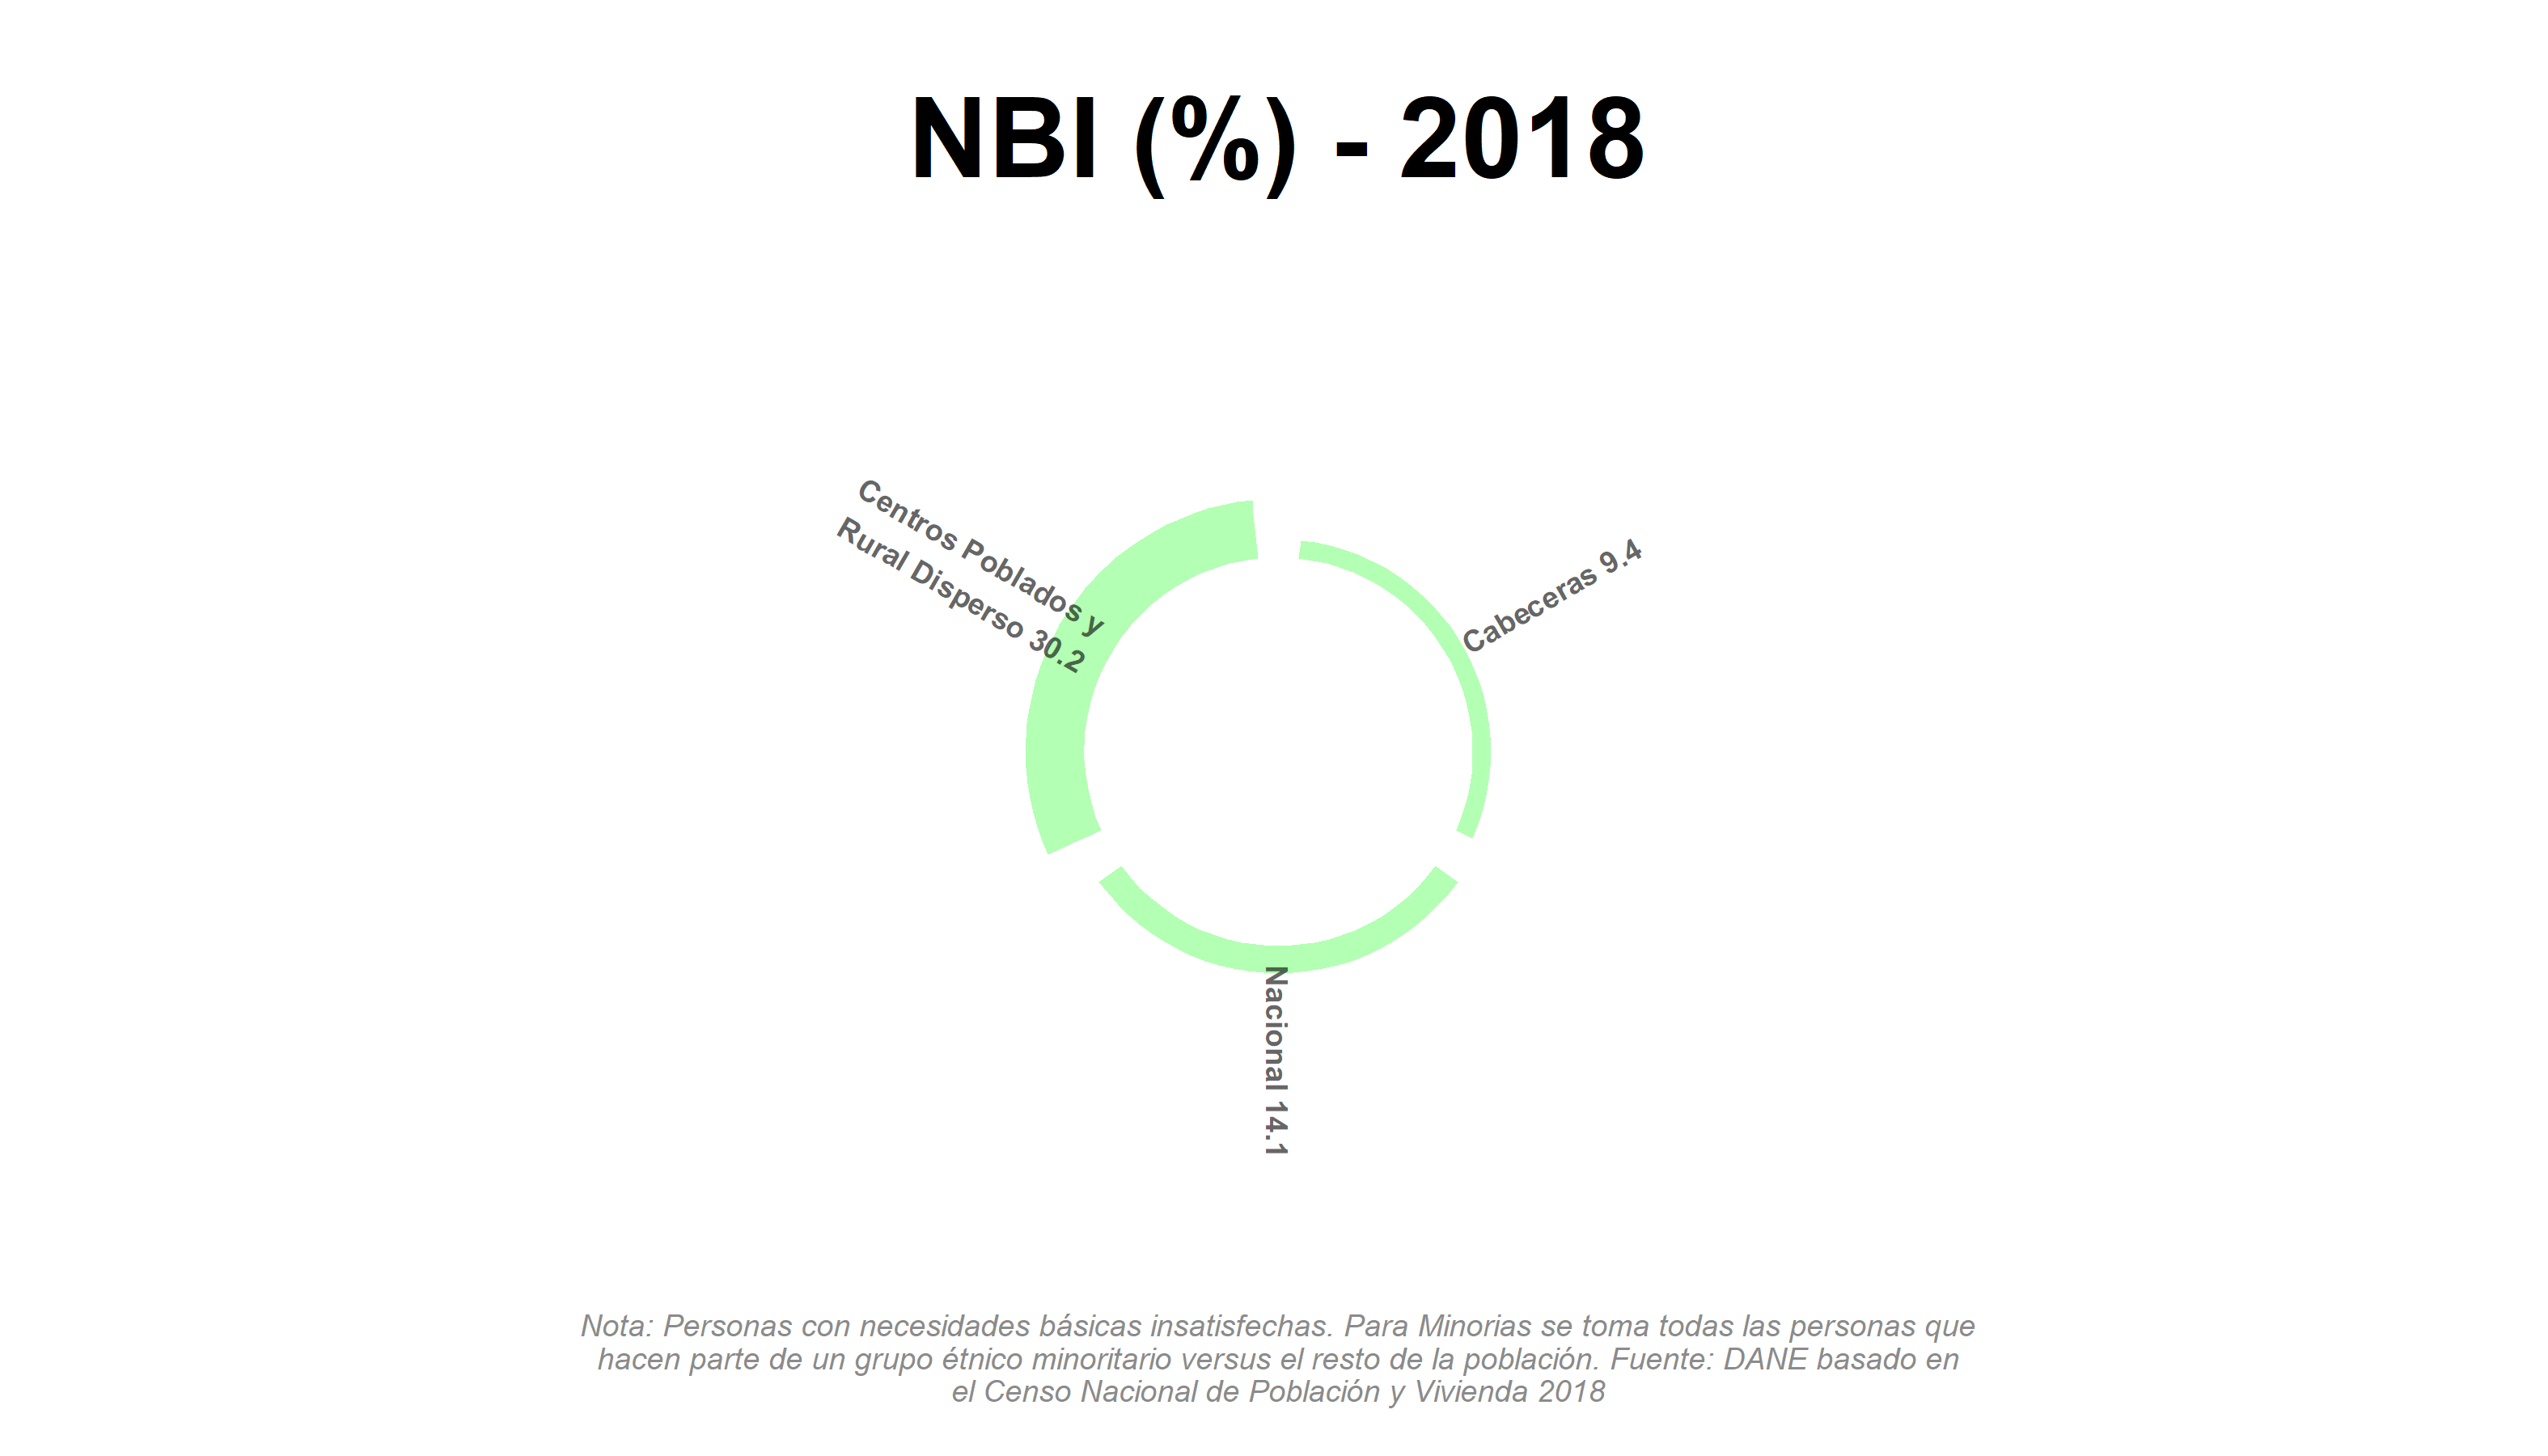
\includegraphics[width=\textwidth,keepaspectratio]{img/var_276_static.png}
        \end{center}
    \end{figure}
            \begin{itemize}
                    \item Los cálculos de las NBI solo están para el 2018 gracias al censo nacional del mismo año, se tiene que a nivel nacional las NBI son del 14.1\%.
                    \item A nivel rural es donde más NBI hay, con un 30.2\%, mientras que las NBI de las cabeceras son del 9.4\%, una diferencia de más del 20\% y siendo las cabeceras menos que el total nacional.n
                    \end{itemize}

\section{Desigualdad}
    \subsection{Indicadores Convencionales}
        \subsubsection{Coeficiente de Gini}

%%%% Include figures
    \begin{figure}[H]
        \caption{Coeficiente de Gini por ciudades \label{map_result_2} }
        \begin{center}
        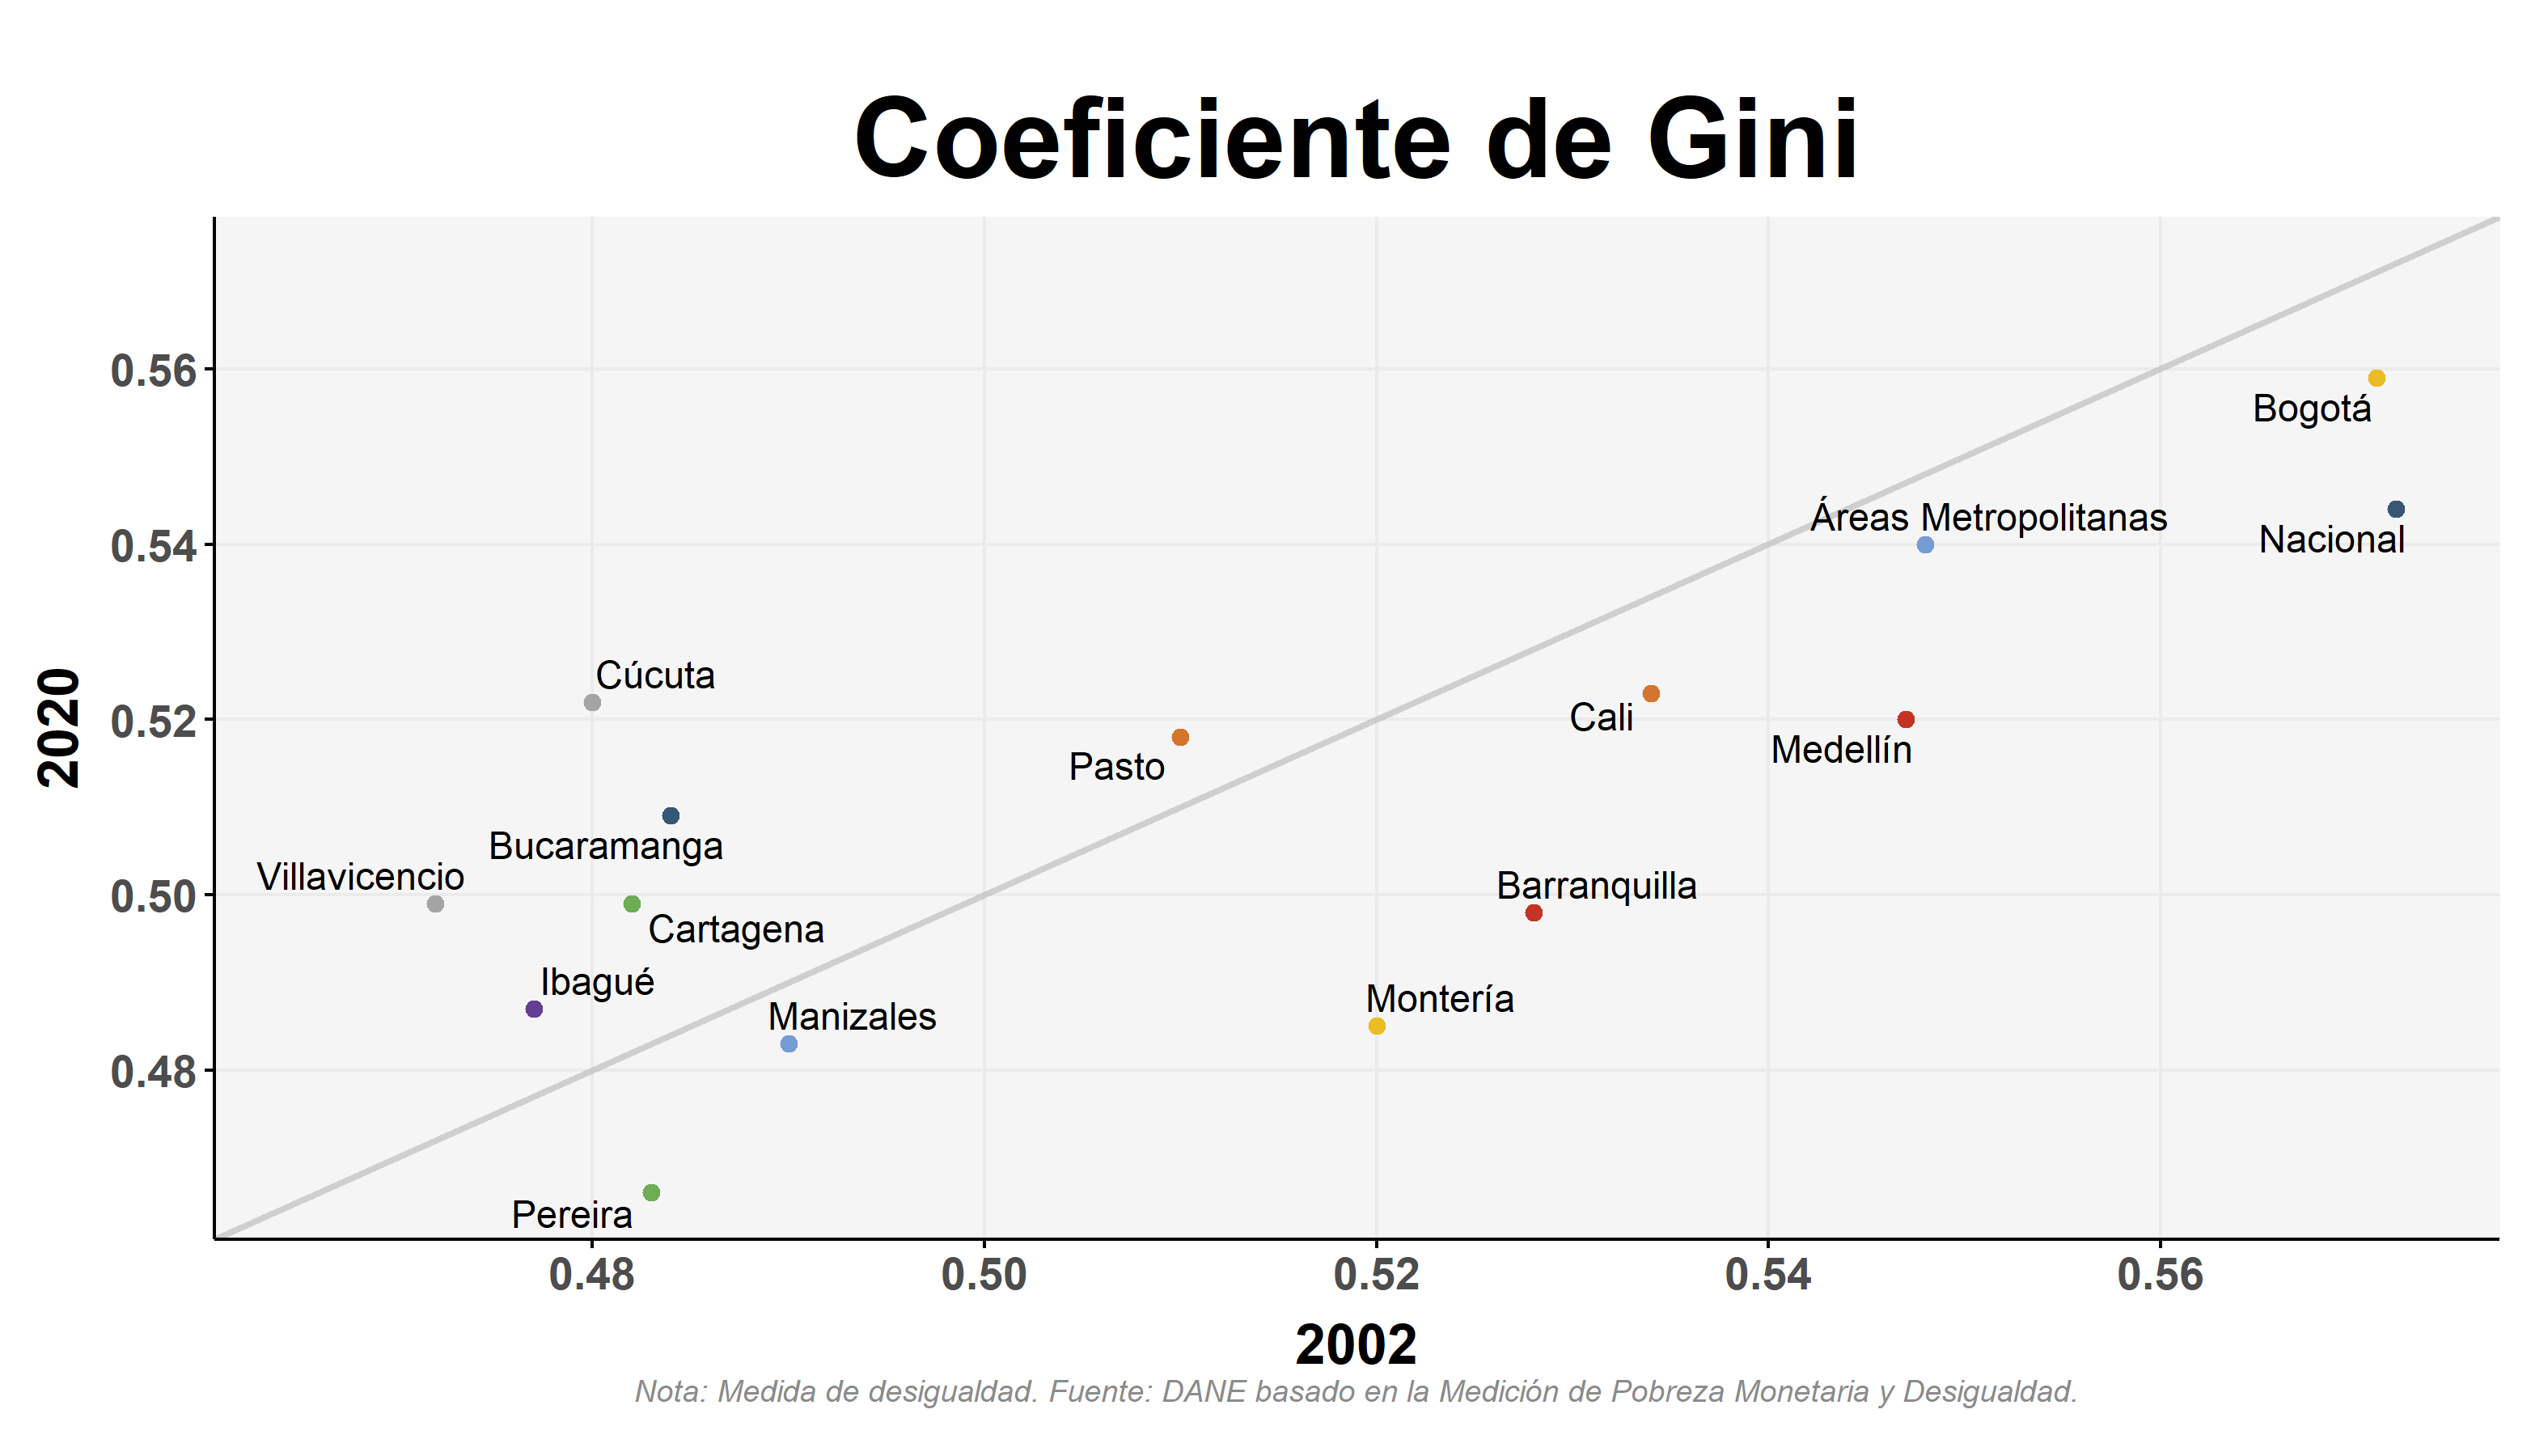
\includegraphics[width=\textwidth,keepaspectratio]{img/var_253_scatter_time.png}
        \end{center}
    \end{figure}
            \begin{itemize}
                    \item En general la mayoría de las ciudades mejoraron sus niveles de desigualdad.
                    \item Cúcuta, Bucaramanga y Villavicencio son las ciudades que aumentaron los niveles de desigualdad que tenían hace casi 20 años.
                    \item Manizáles, Bogotá y Pasto se podría decir que se mantuvieron cerca de los niveles de desigualdad que tenían en 2002.
                    \item Bogotá sigue siendo la ciudad con mayor nivel de desigualdad, mientras que la de menor es Pereira.
                    \end{itemize}

%%%% Include figures
    \begin{figure}[H]
        \caption{Coeficiente de Gini por departamentos \label{map_result_2} }
        \begin{center}
        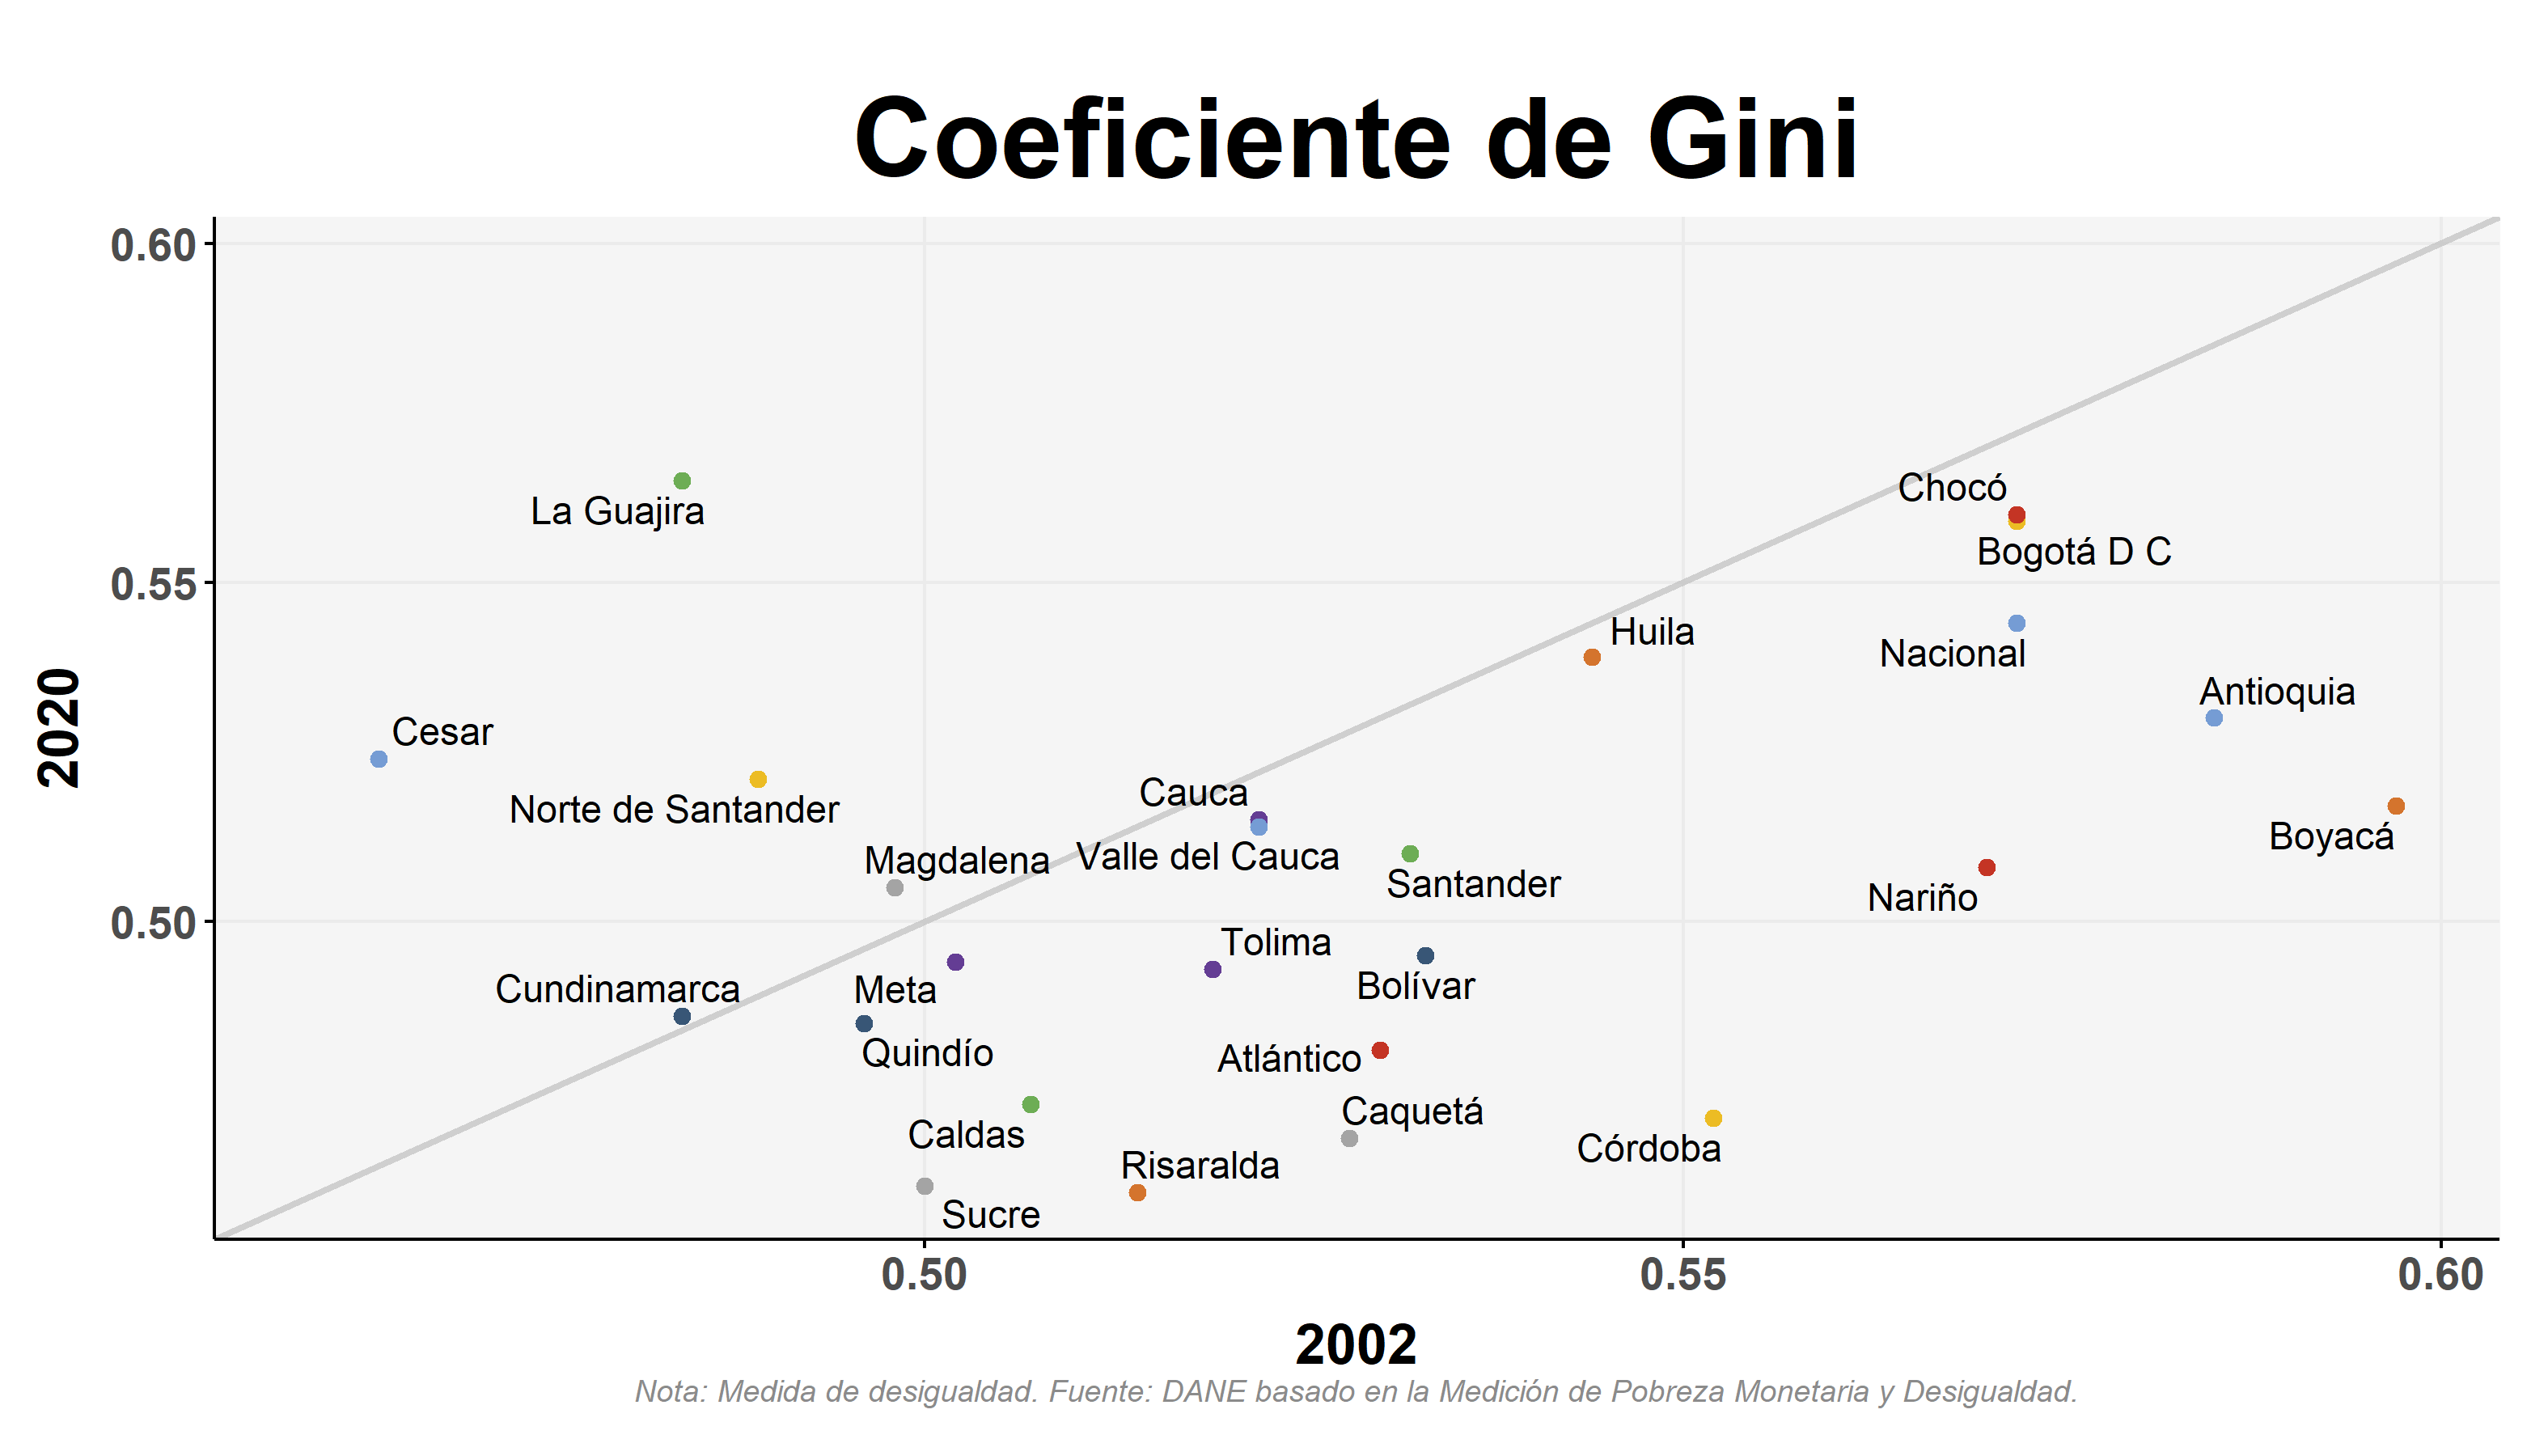
\includegraphics[width=\textwidth,keepaspectratio]{img/var_254_scatter_time.png}
        \end{center}
    \end{figure}
            \begin{itemize}
                    \item Gran parte de los territorios mostró una mejorías en la desigualdad.
                    \item Departamentos como Huila, Cauca y Cundinamarca están cerca de los niveles reportados 18 años atrás.
                    \item La Guajira a pesar de en el 2002 ser de los departamentos con menor desigualdad, para el 2020 es el de mayor según el coeficiente de Gini.
                    \item Risaralda es el dpto con menor desigualdad, aunque cabe mencionar que la distribución no es tan amplia (0.45 a 0.55).
                    \end{itemize}

%%%% Include figures
    \begin{figure}[H]
        \caption{Coeficiente de Gini por zonas y nacional \label{map_result_2} }
        \begin{center}
        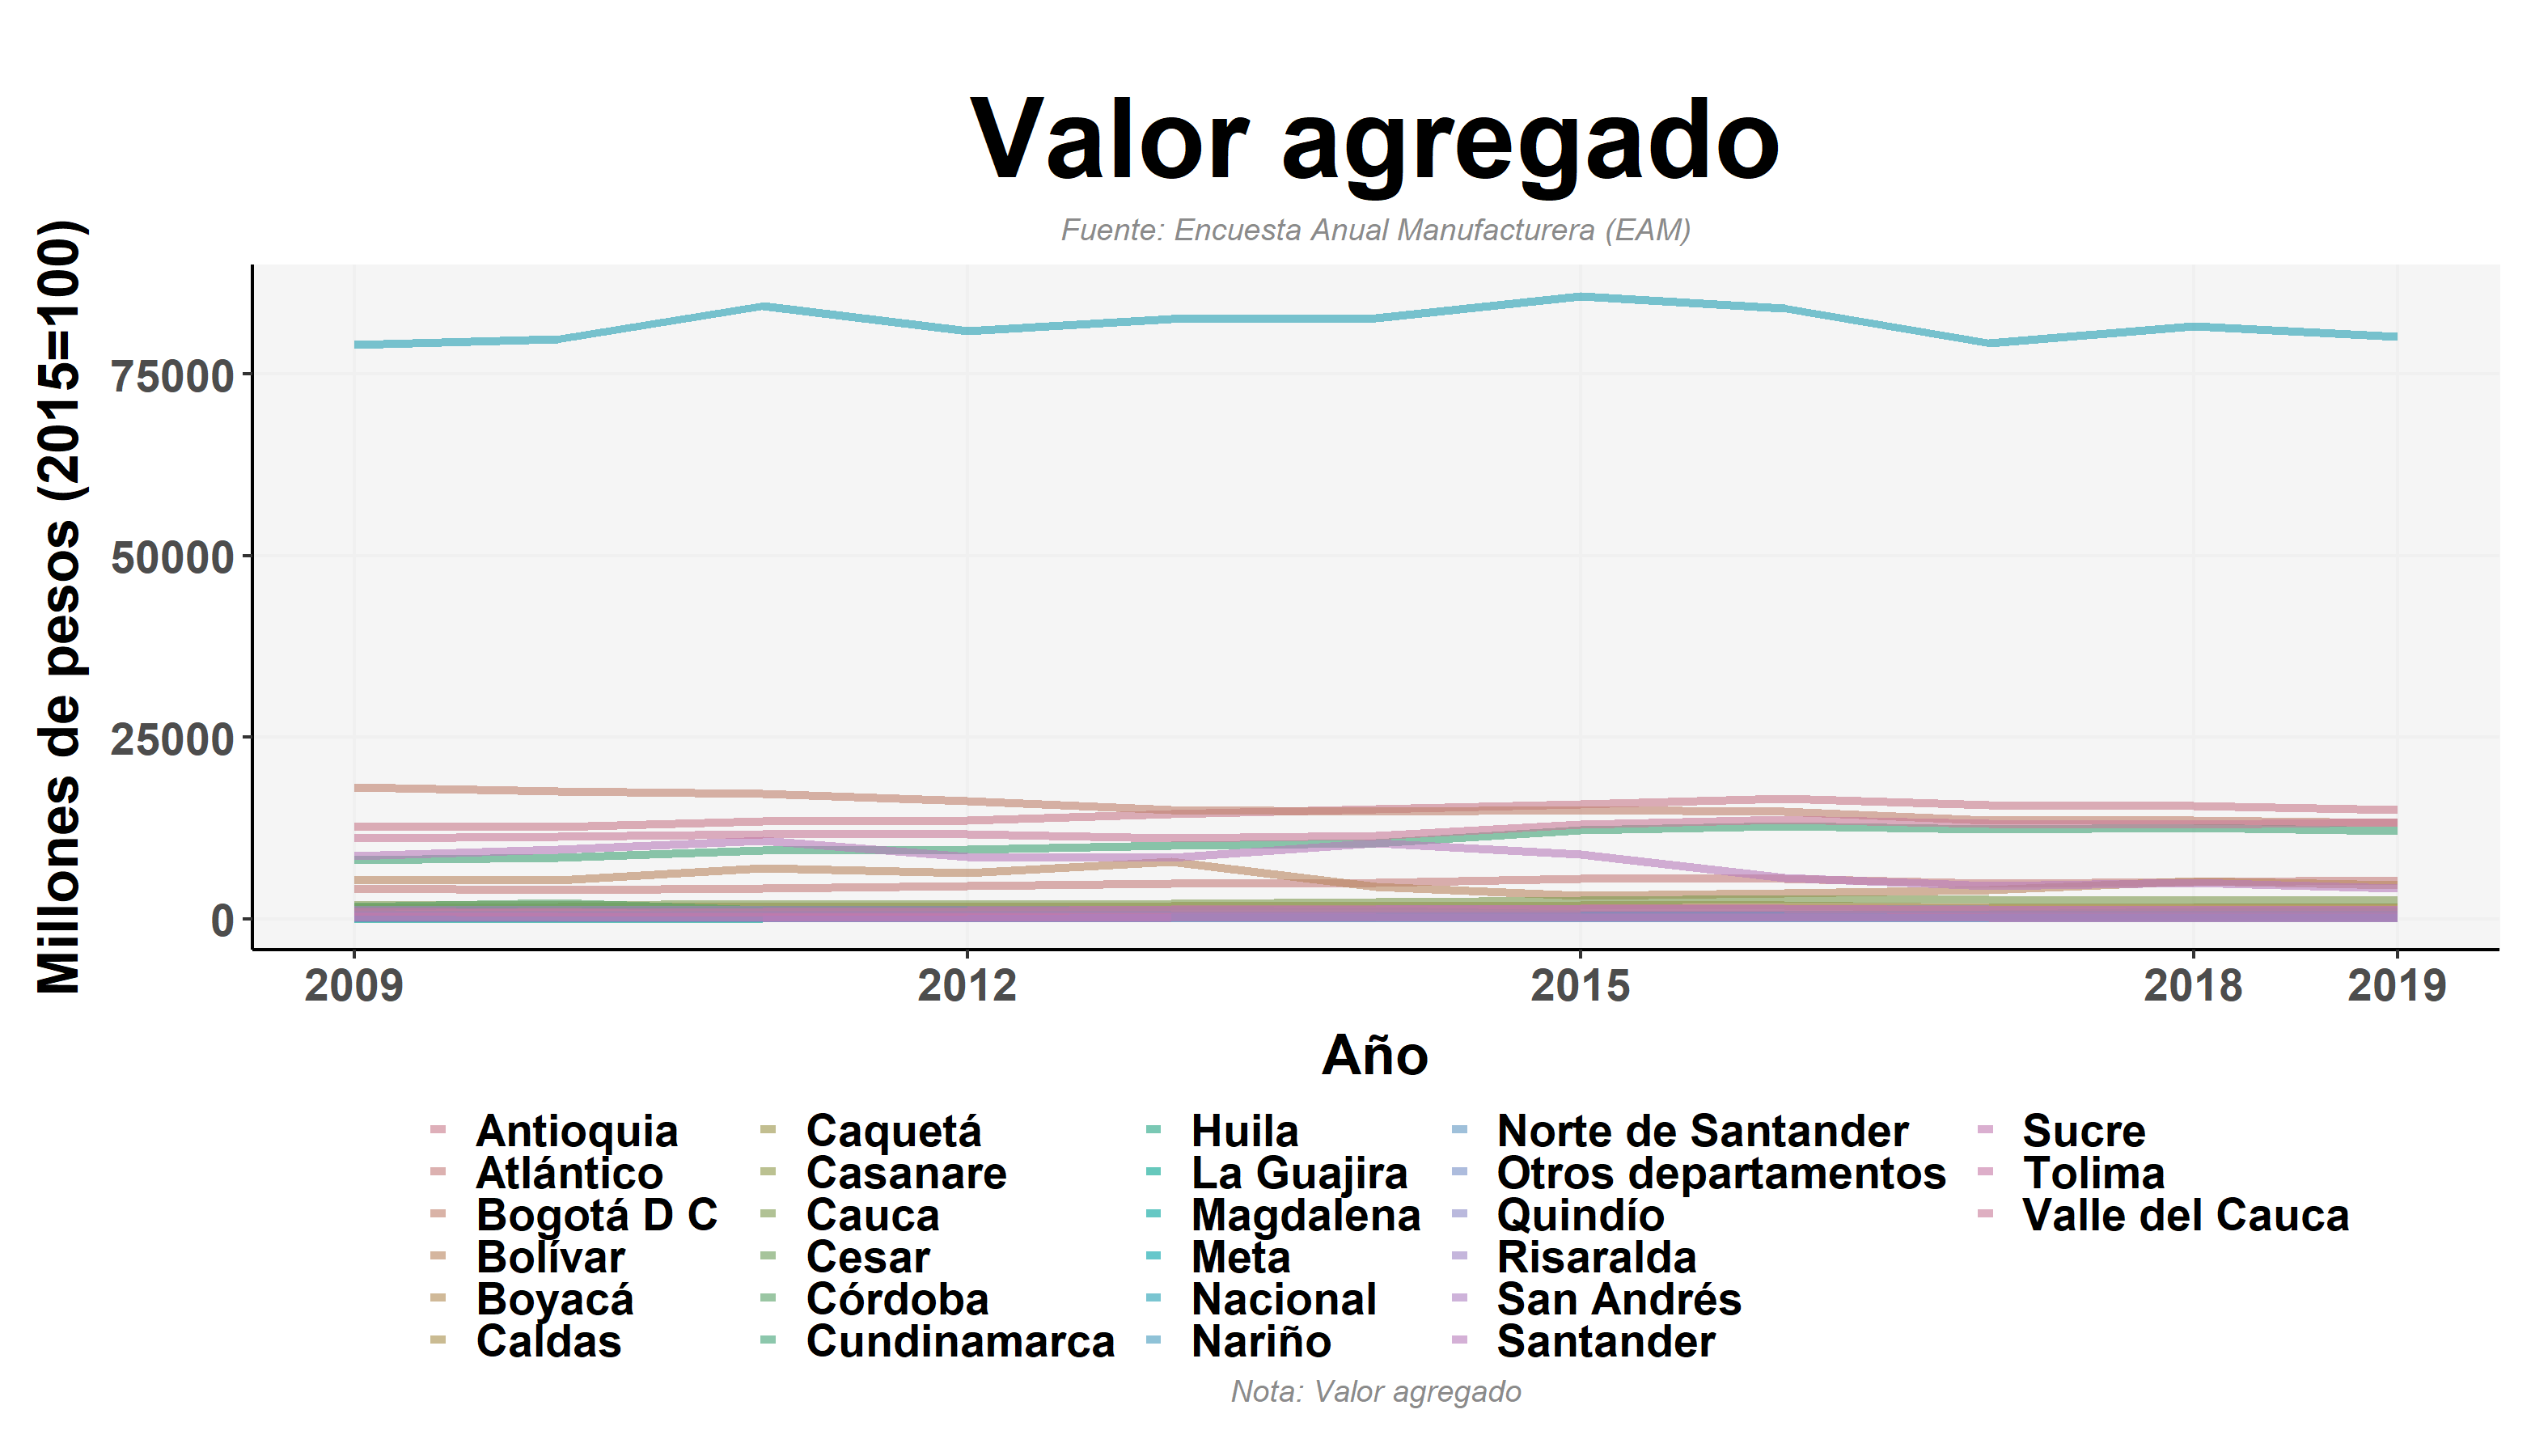
\includegraphics[width=\textwidth,keepaspectratio]{img/var_256_trend.png}
        \end{center}
    \end{figure}
            \begin{itemize}
                    \item A nivel de zonas se encontró que desde el 2008 se veía una tendencia a la baja hasta el 2017 donde volvió a aumentar, a excepción de la zona rural, que se intensificó en el 2020.
                    \item La zona rural ha mostrado tener los niveles de desigualdad más bajo, manteniendo niveles similares desde el 2014.
                    \item Para el 2020 las cabeceras y a nivel nacional tuvieron una menor brecha, alcanzando niveles similares.
                    \item Para las otras cabeceras el comportamiento es igual que el de las cabeceras, pero con menor intensidad en el caso del 2020.
                    \end{itemize}

\section{Características de las Viviendas}
    \subsection{Calidad de los Materiales}
        \subsubsection{Material de la Pared}

%%%% Include figures
    \begin{figure}[H]
        \caption{Viviendas con pared de ladrillo por departamentos para 2020 \label{map_result_2} }
        \begin{center}
        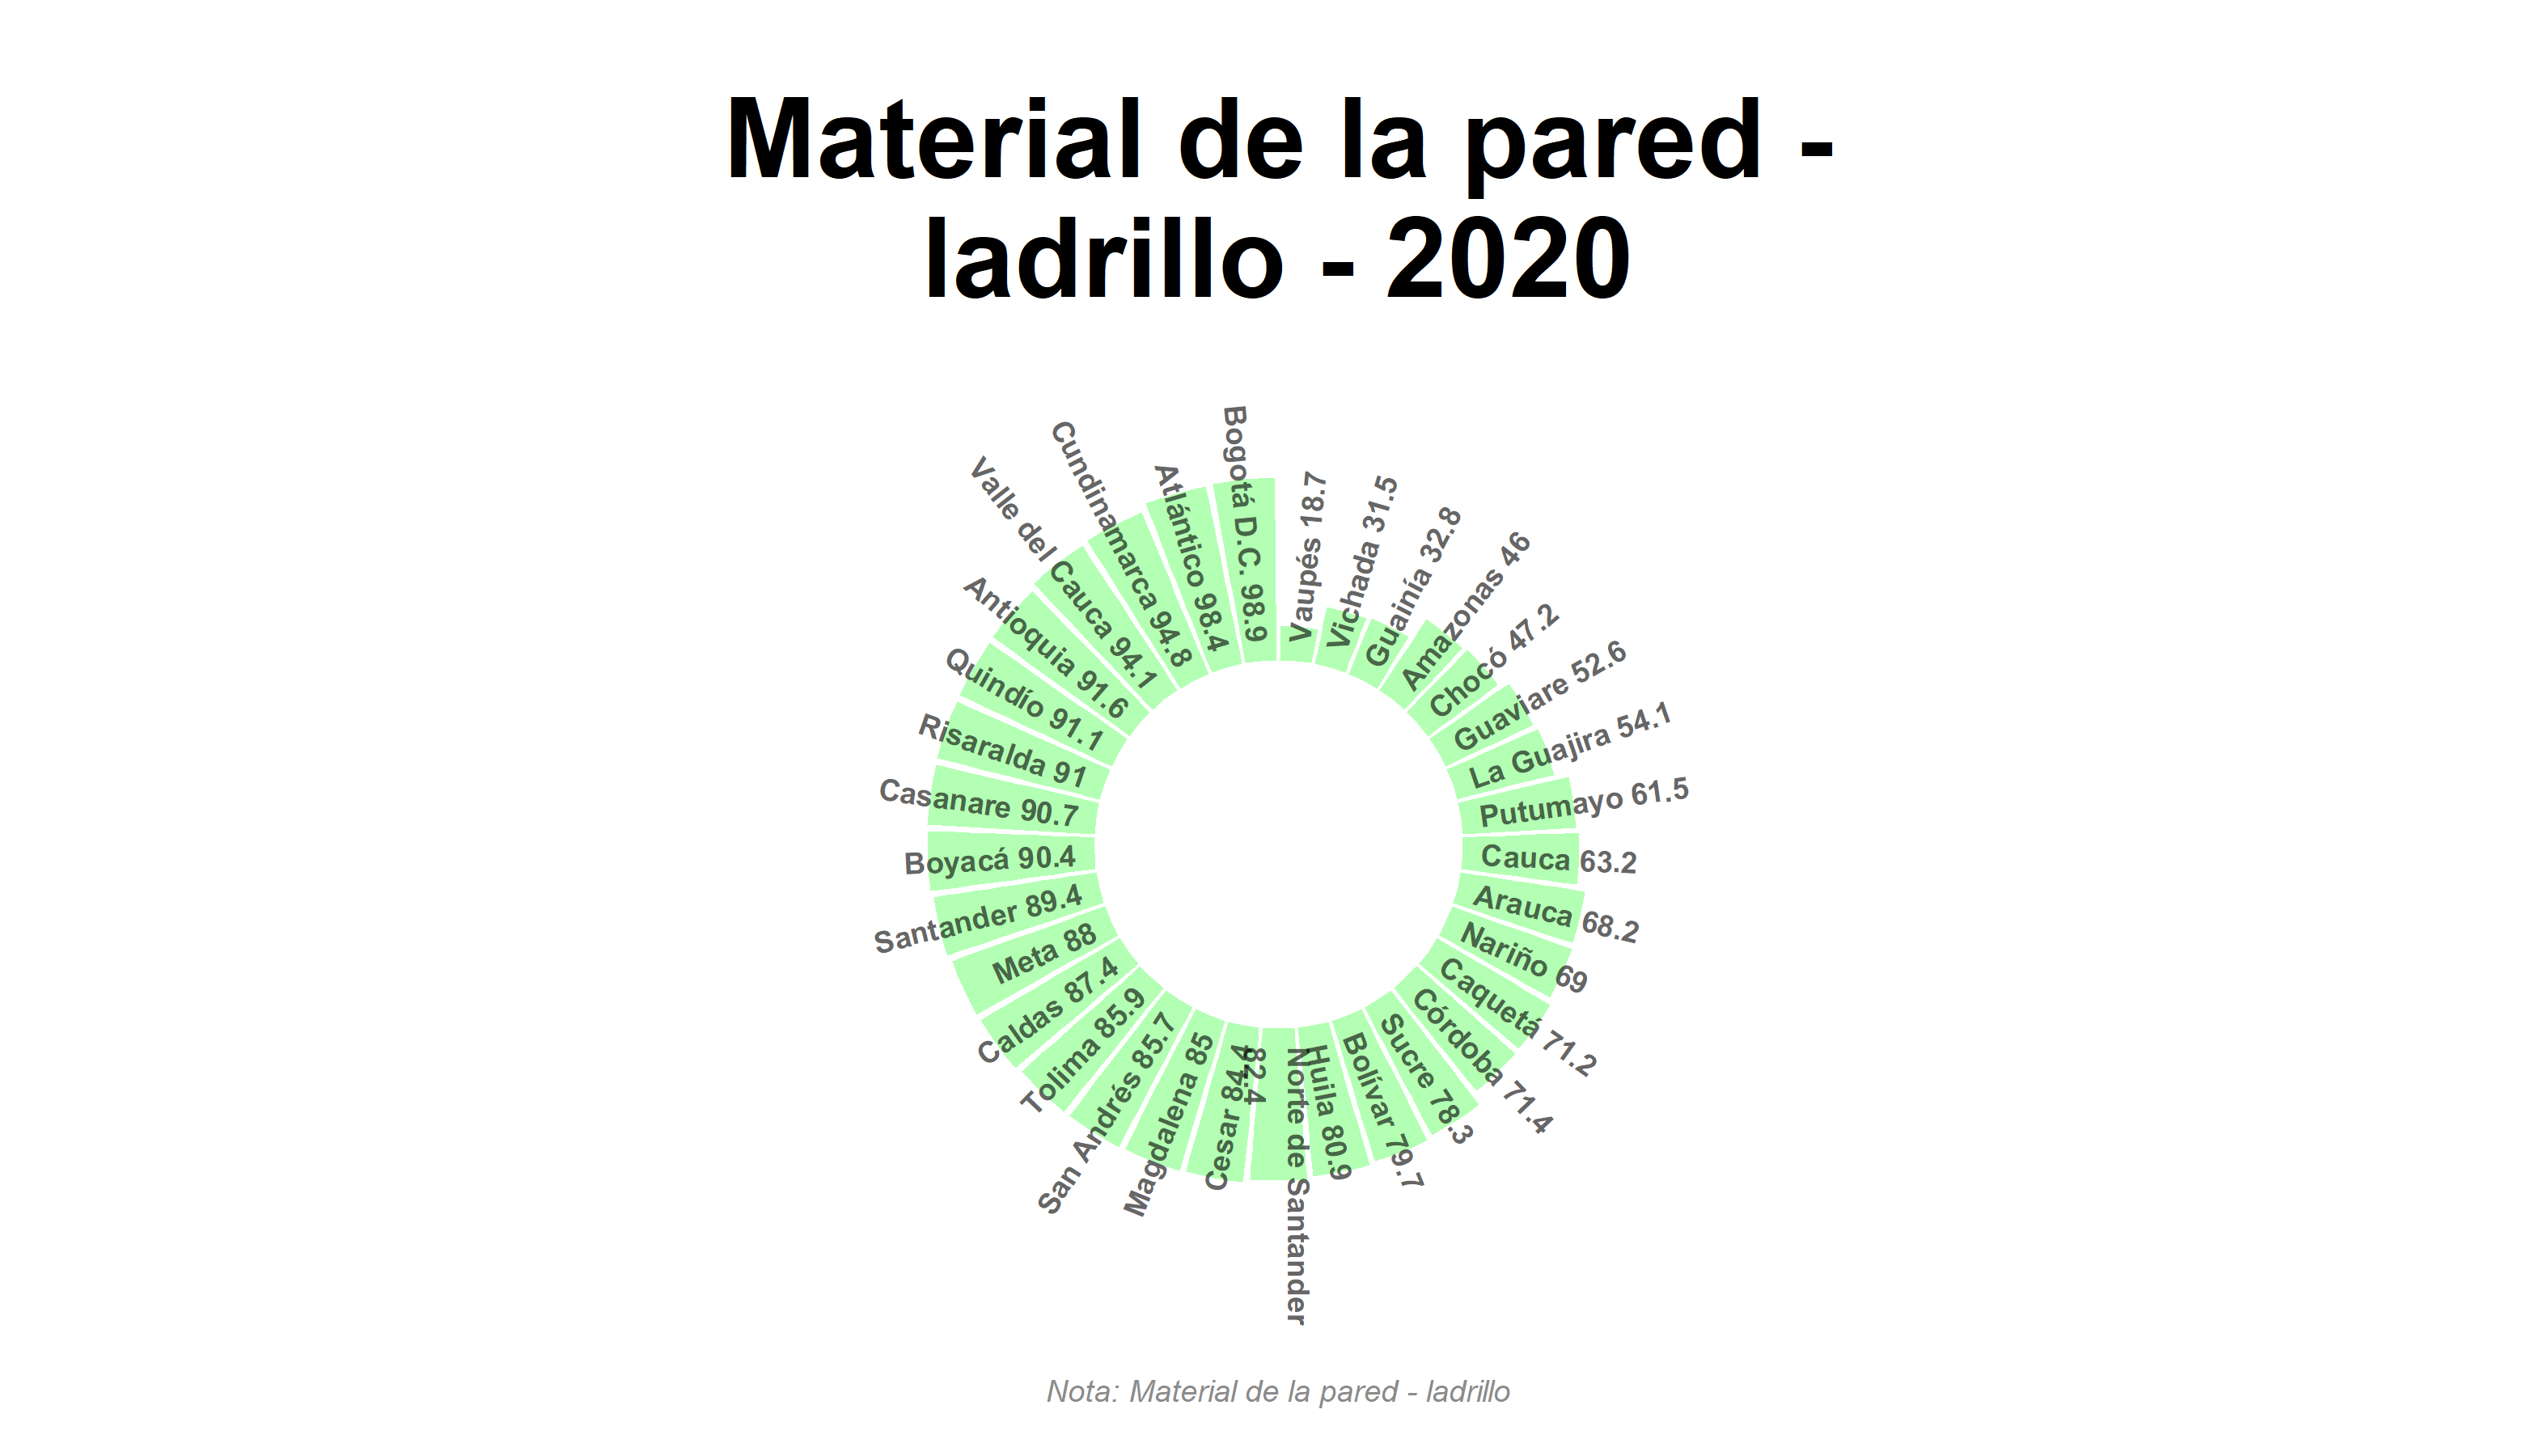
\includegraphics[width=\textwidth,keepaspectratio]{img/var_150_static.png}
        \end{center}
    \end{figure}
            \begin{itemize}
                    \item El ladrillo es el material más usado para las paredes, estando en más del 60\% de las viviendas en la mayoría de los dptos, siendo más de la mitad de estos por encima del 80\%.
                    \item La diferencia entre el territorio con más viviendas con paredes de ladrillo y el de menos es de poco más del 80\% (Bogotá - Vaupés).
                    \item Los departamentos que menos viviendas en este material tienen están por debajo del 35\%, teniendo el caso de Vaupés que solo el 19\% de las viviendas tienen paredes en este material.
                    \end{itemize}

%%%% Include figures
    \begin{figure}[H]
        \caption{Viviendas con pared de ladrillo por zonas \label{map_result_2} }
        \begin{center}
        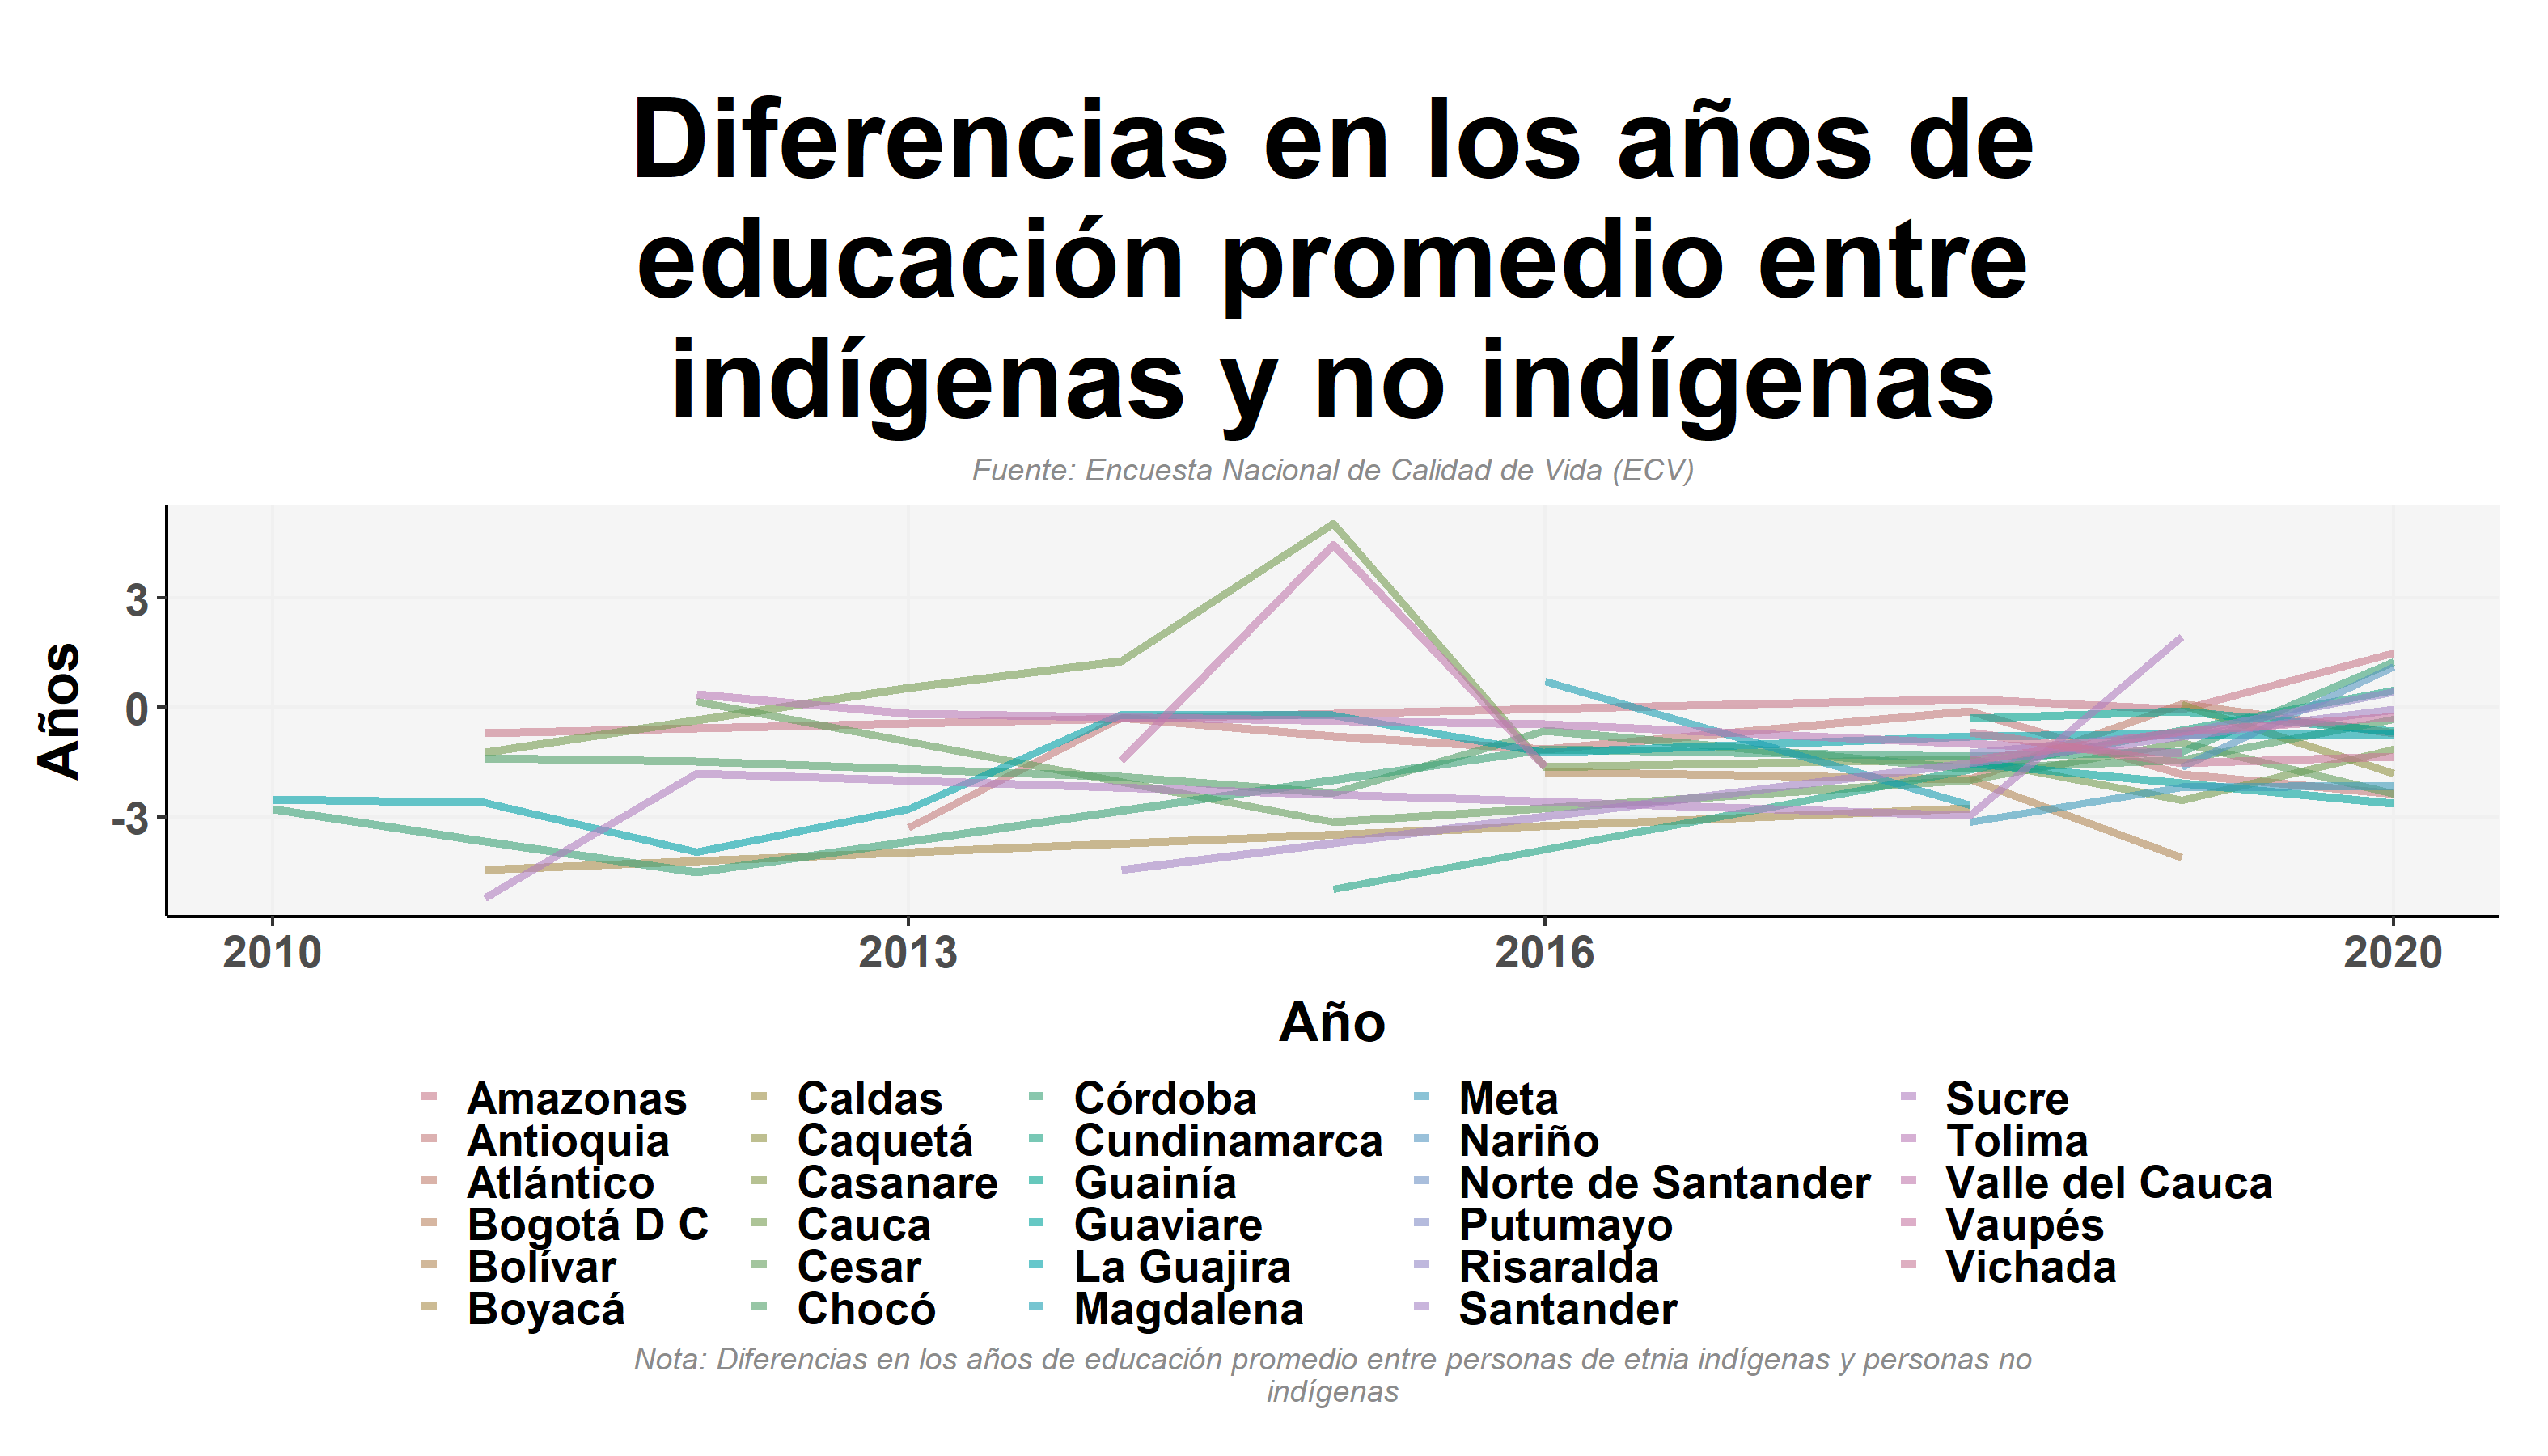
\includegraphics[width=\textwidth,keepaspectratio]{img/var_151_trend.png}
        \end{center}
    \end{figure}
            \begin{itemize}
                    \item El material es predominantemente usado en las cabeceras, estando por encima del 90\% de las viviendas, mientras que en la zona rural es cerca del 60\%.
                    \item El uso del material estaba aumentando en la zonas rurales, pero a partir del 2016 disminuyó a tal nivel que para 2020 está a los niveles que se tenían en el 2010.
                    \end{itemize}

%%%% Include figures
    \begin{figure}[H]
        \caption{Viviendas con pared de madera por departamentos para 2020 \label{map_result_2} }
        \begin{center}
        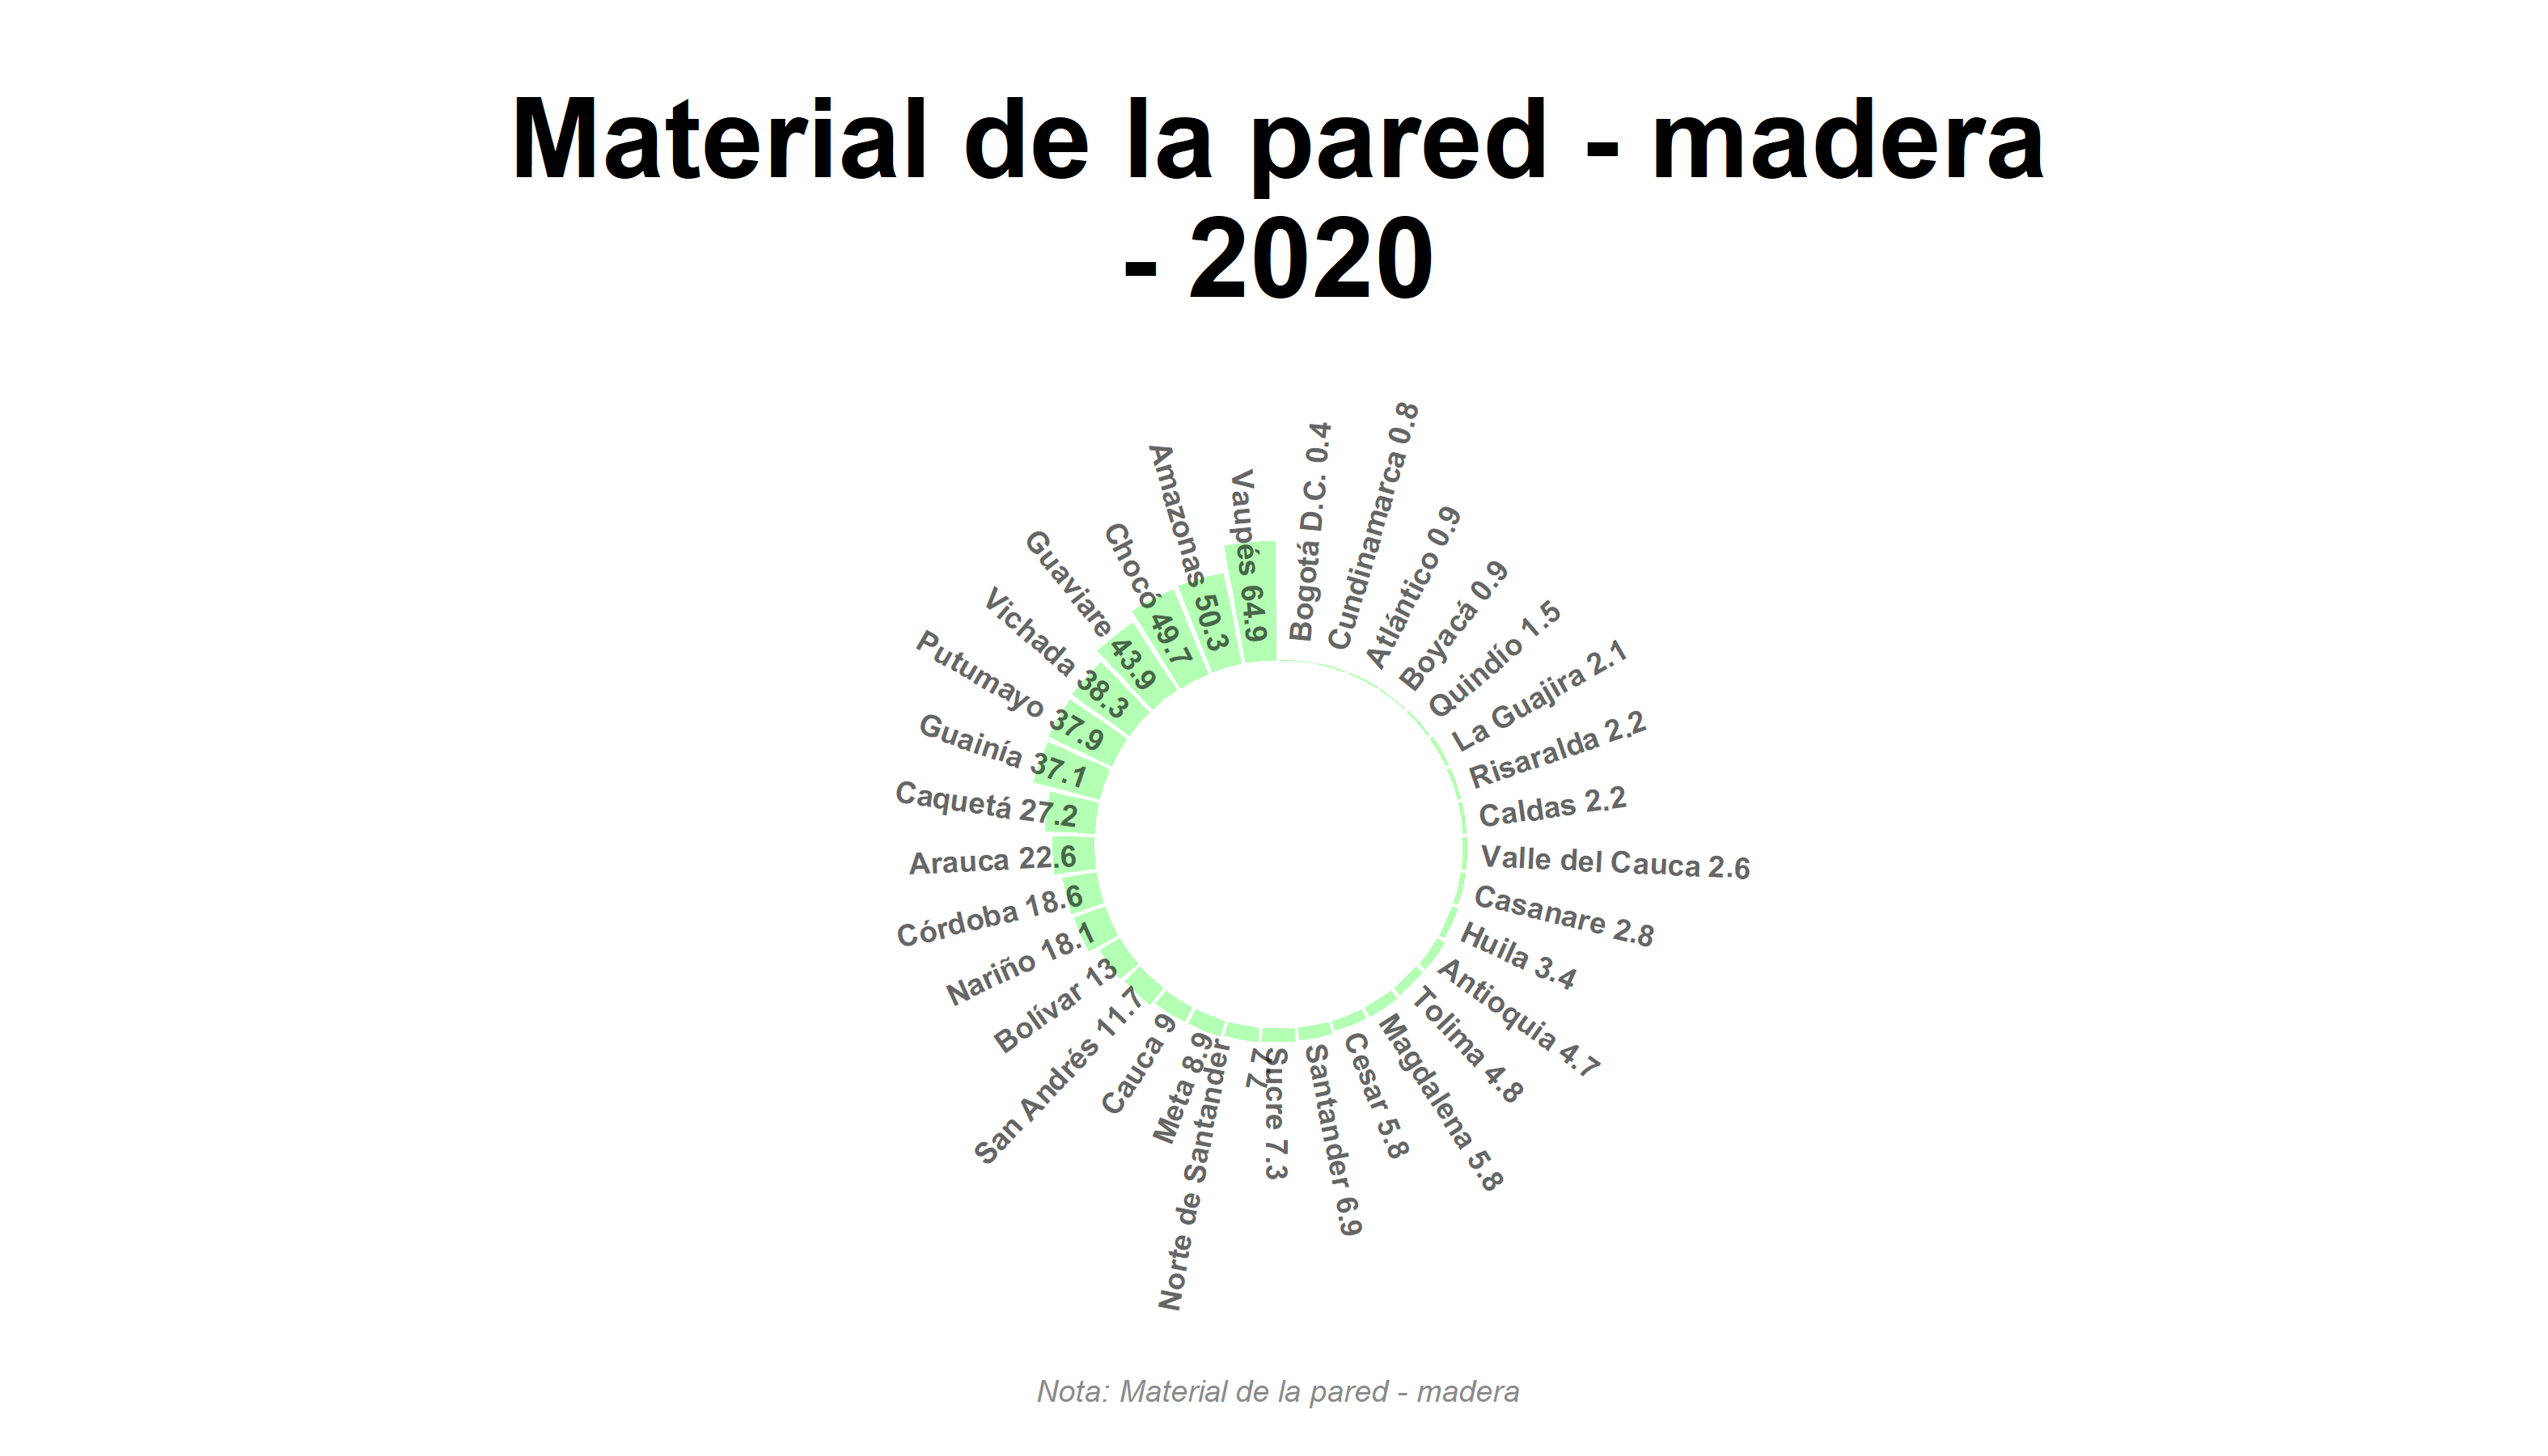
\includegraphics[width=\textwidth,keepaspectratio]{img/var_160_static.png}
        \end{center}
    \end{figure}
            \begin{itemize}
                    \item Las paredes de madera son el segundo material más usado para las paredes, aunque la mitad de los territorios están por debajo del 10\% de las viviendas, los últimos cuatro están por encima del 40\%
                    \item El de menor viviendas en este material es Bogotá con menos del 1\%, mientras que el de más es Vaupés con cerca del 65\%.
                    \item La zonas en las que más se usa el materias son en la Amazonia y los llanos orientales (gráfica map 160 - 2020) con niveles por encima del 20\% de las viviendas..
                    \end{itemize}

%%%% Include figures
    \begin{figure}[H]
        \caption{Viviendas con pared de madera por zonas \label{map_result_2} }
        \begin{center}
        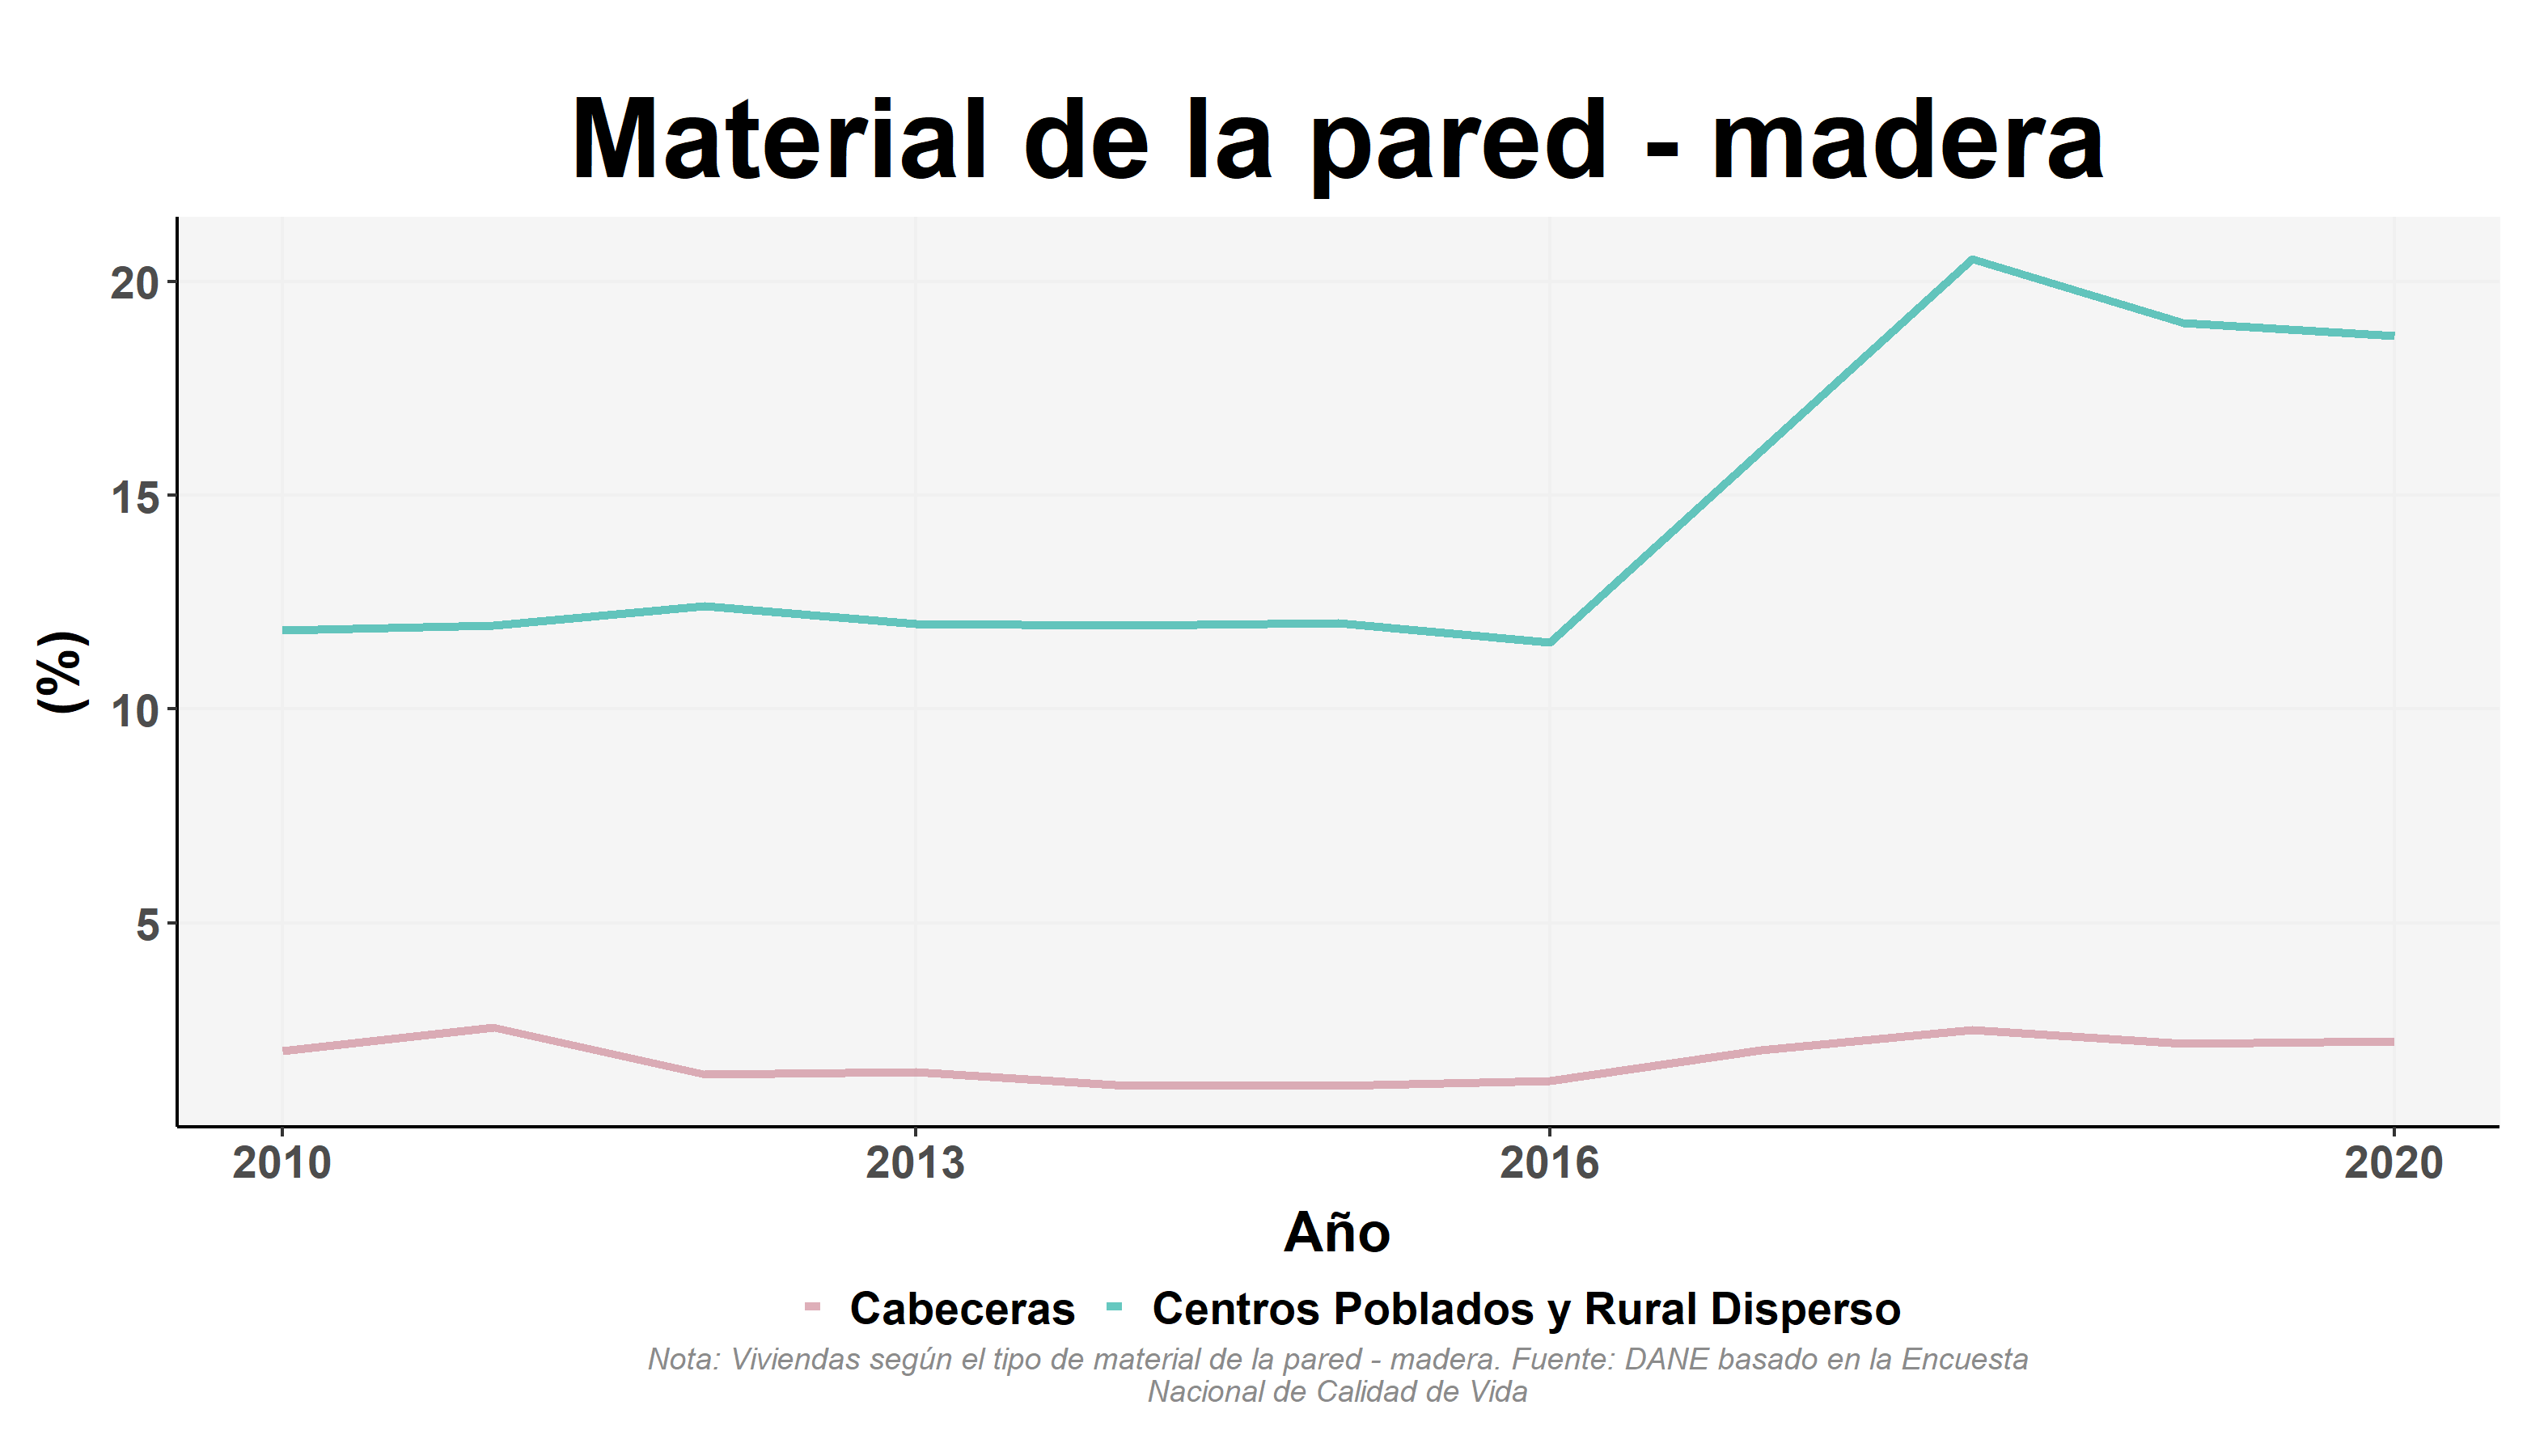
\includegraphics[width=\textwidth,keepaspectratio]{img/var_161_trend.png}
        \end{center}
    \end{figure}
            \begin{itemize}
                    \item El material es usado predominantemente en las zonas rurales, cerca del 20\% de las viviendas, mientras que en las cabeceras está por debajo del 5\%.
                    \item El uso de este material aumentó desde 2016 para la zona rural, en las cabeceras se ha mantenido constante.
                    \end{itemize}

%%%% Include figures
    \begin{figure}[H]
        \caption{Viviendas con pared de bahareque revocado por departamentos para 2020 \label{map_result_2} }
        \begin{center}
        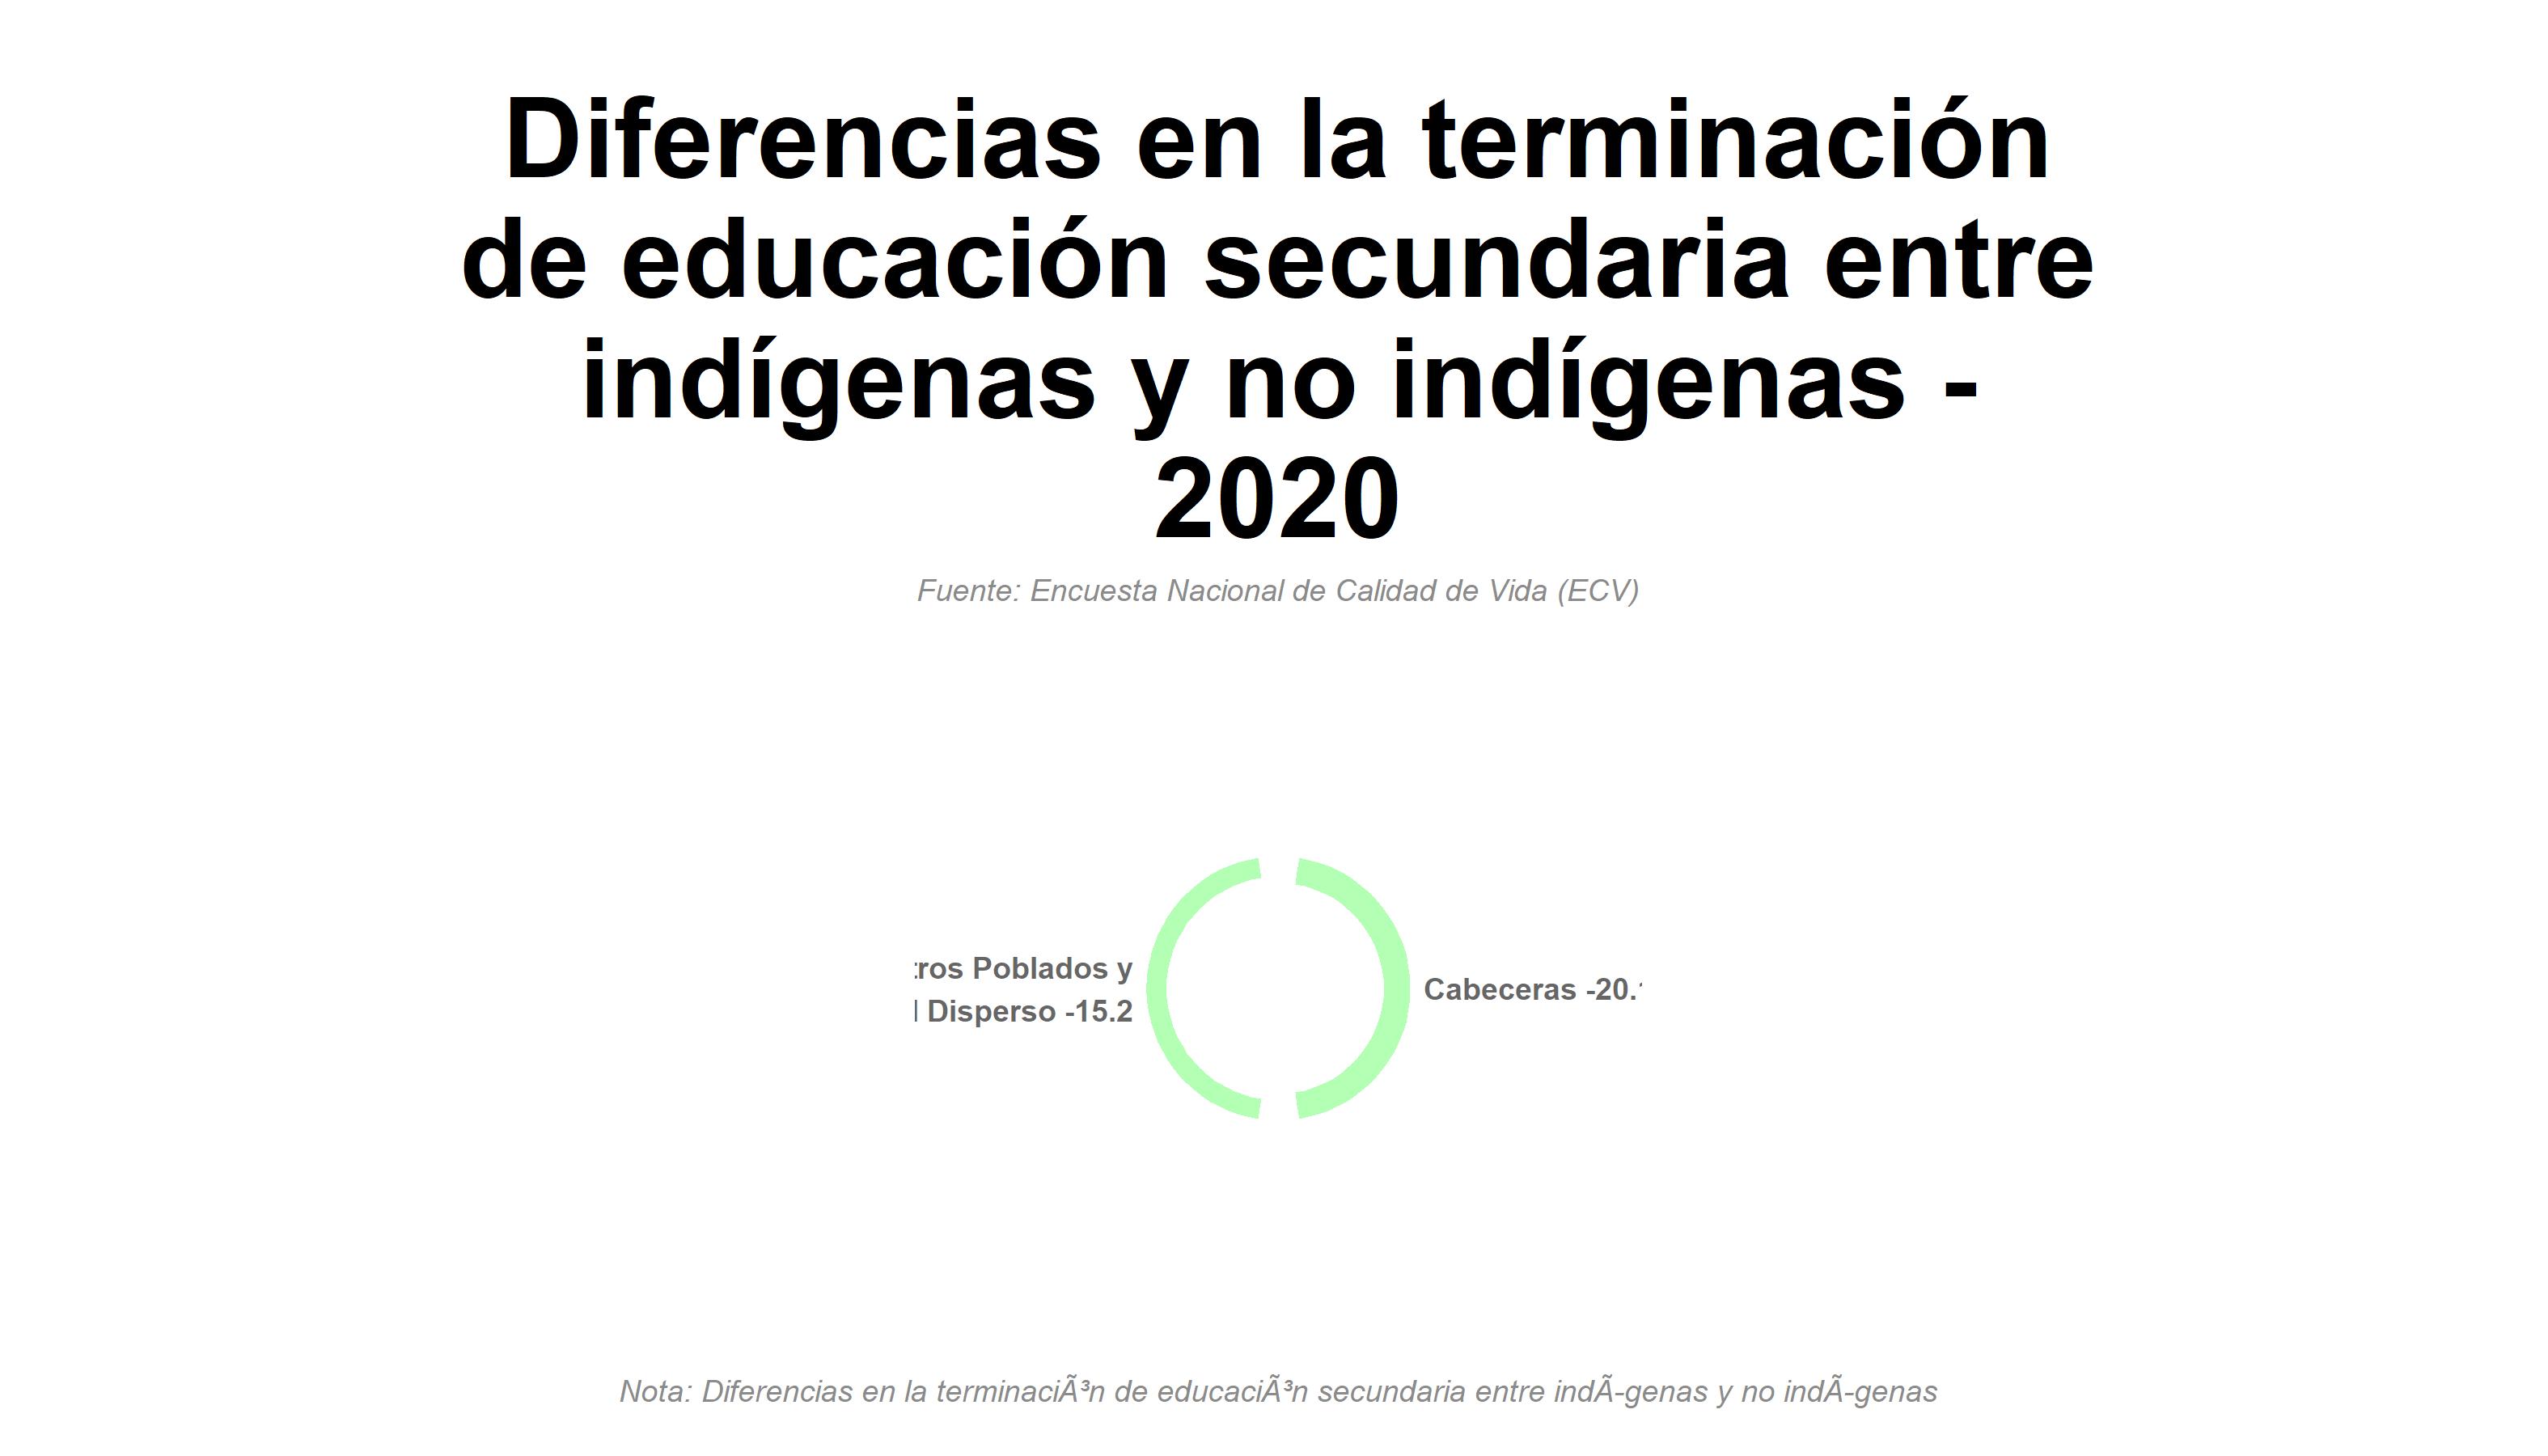
\includegraphics[width=\textwidth,keepaspectratio]{img/var_154_static.png}
        \end{center}
    \end{figure}
            \begin{itemize}
                    \item Aunque es el tercer material más usado encontramos que solo 3 departamentos tienen niveles por encima del 10\% de las viviendas, Huila, La Guajira y Guainía, siendo este último el de mayor con un 13.8\%.
                    \item La mitad de los departamentos tienen menos del 1\% de las viviendas, o valores cercanos a cero, con paredes en este material.
                    \end{itemize}

%%%% Include figures
    \begin{figure}[H]
        \caption{Viviendas con pared de bahareque revocado por zonas \label{map_result_2} }
        \begin{center}
        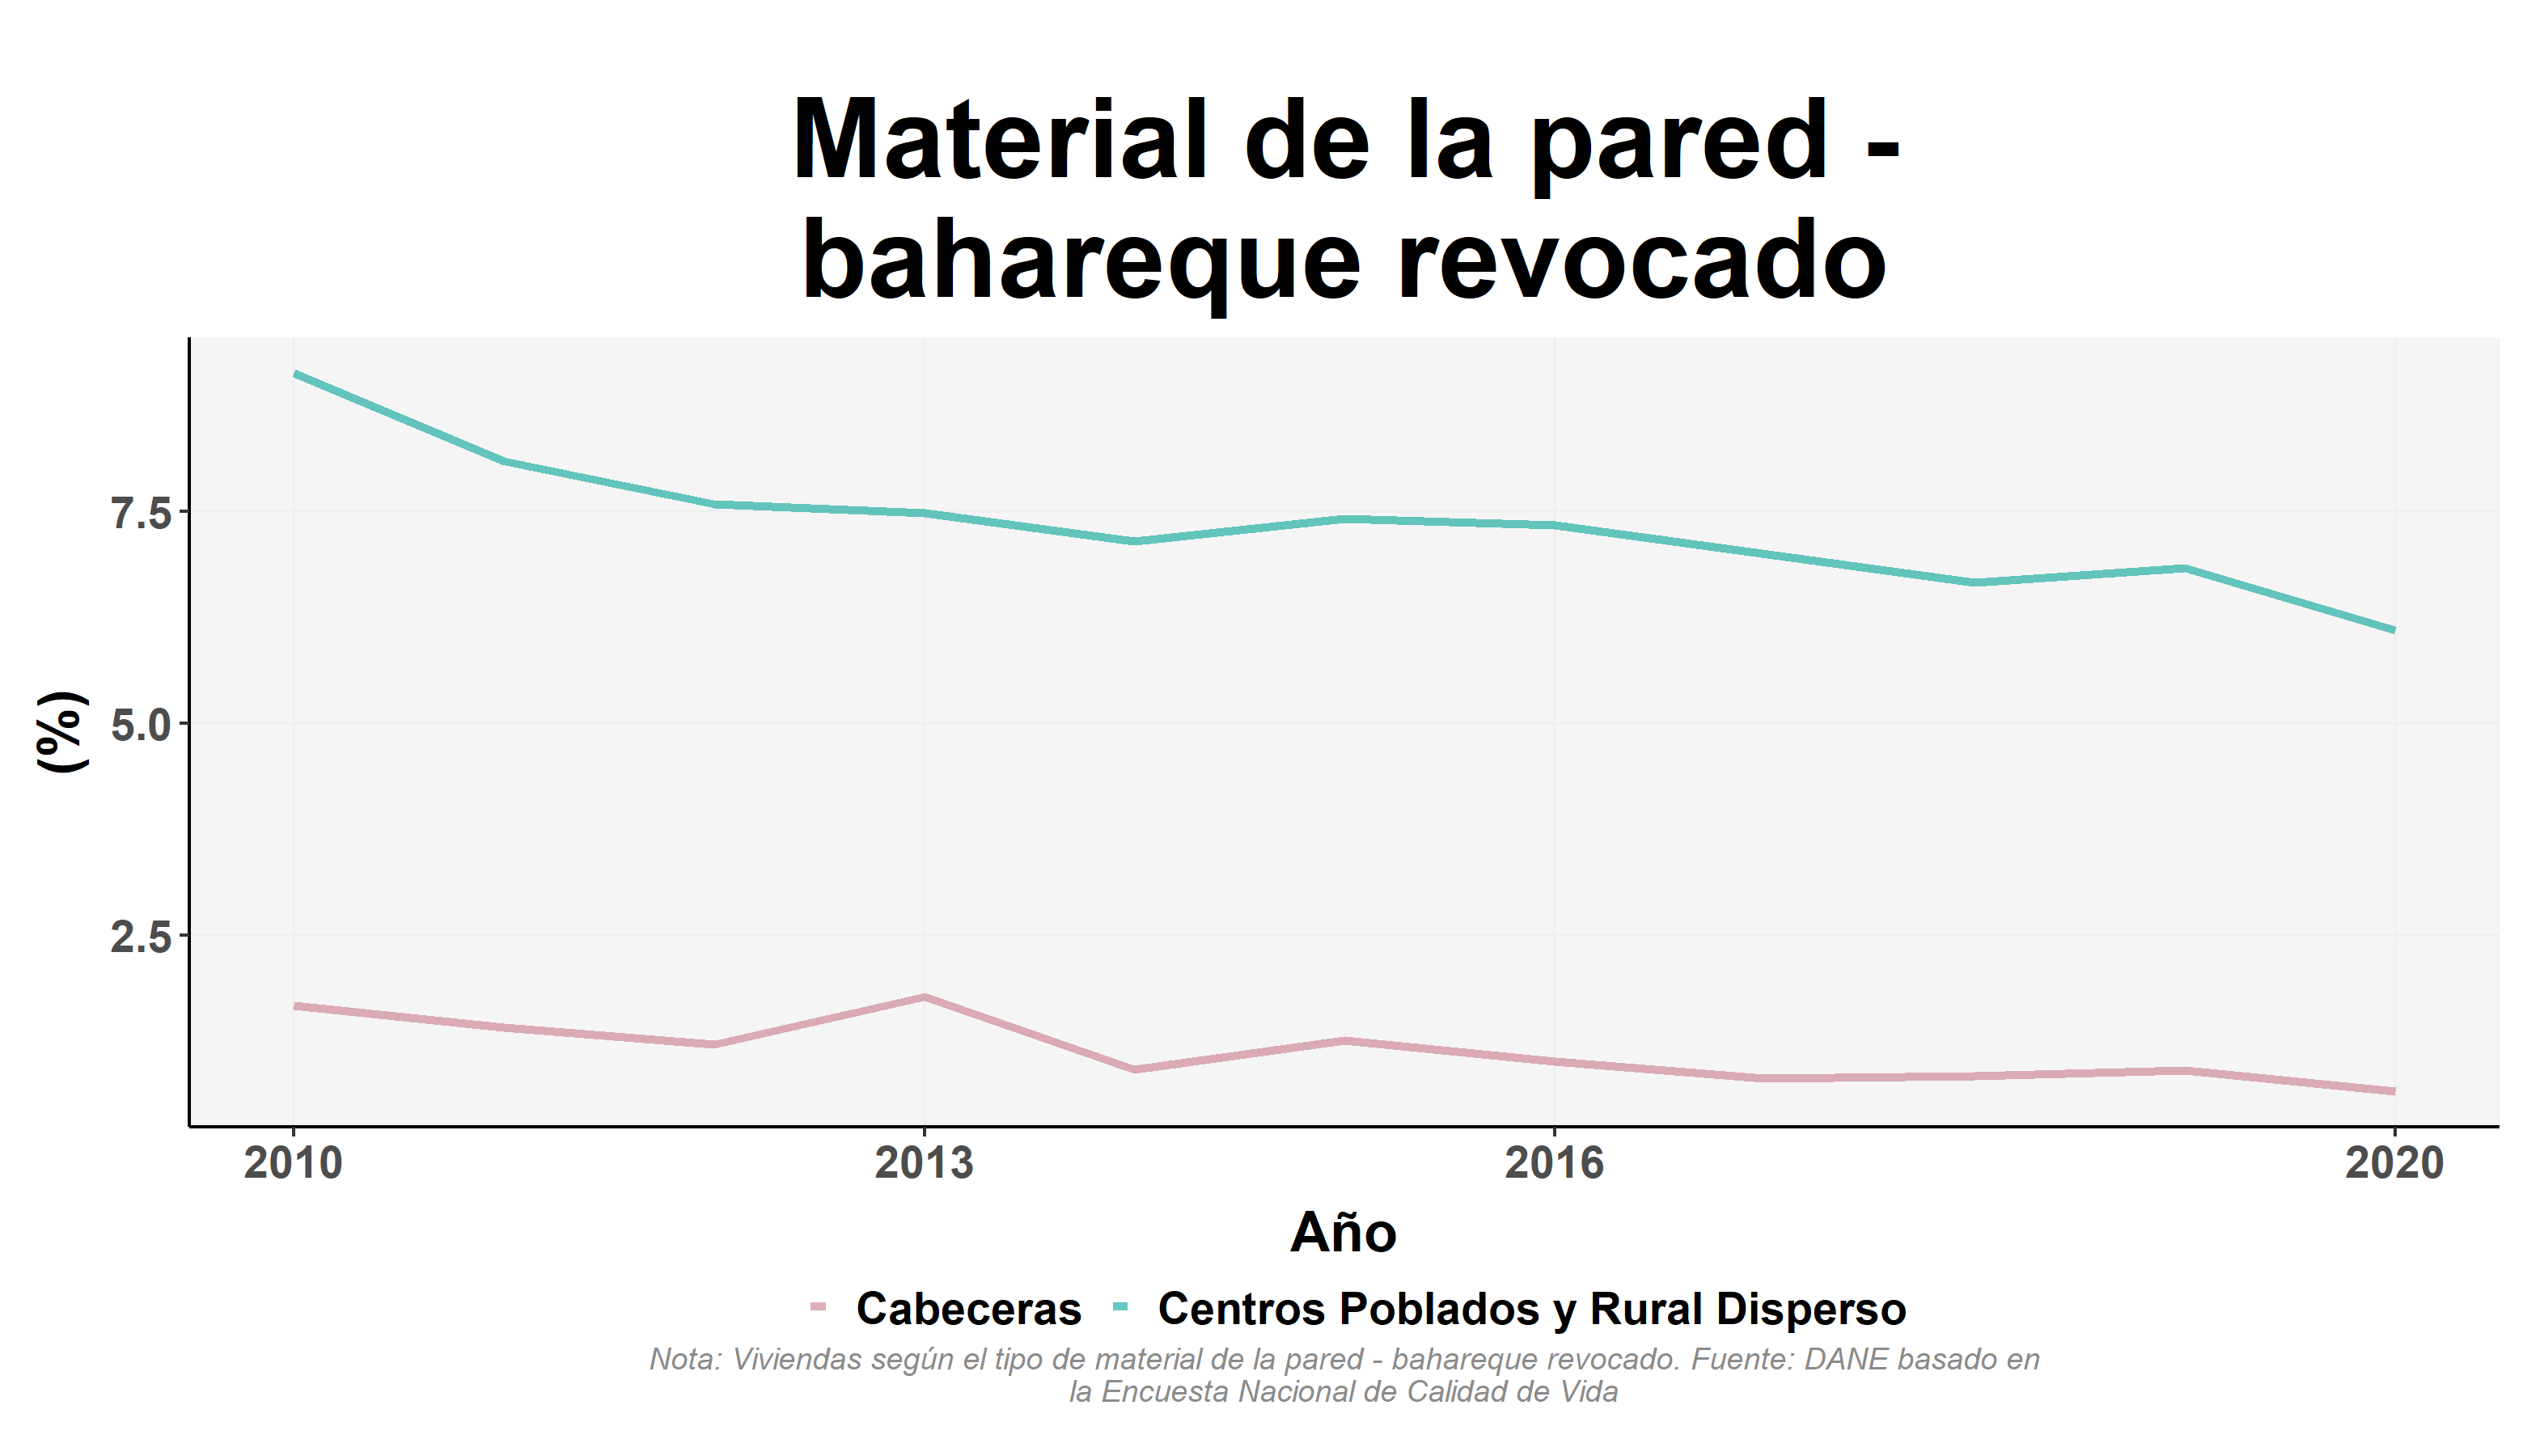
\includegraphics[width=\textwidth,keepaspectratio]{img/var_155_trend.png}
        \end{center}
    \end{figure}
            \begin{itemize}
                    \item El material es predominantemente usado en las zonas rurales, cerca de un 6\% para 2020, mientras que en las cabeceras es menos del 1\%.
                    \item El uso de este material ha venido disminuyendo en ambas zonas, pero es más notorio en el área rural, donde en 2010 estaba por encima del 8\%.
                    \end{itemize}

%%%% Include figures
    \begin{figure}[H]
        \caption{Viviendas con pared de bahareque no revocado por departamentos para 2020 \label{map_result_2} }
        \begin{center}
        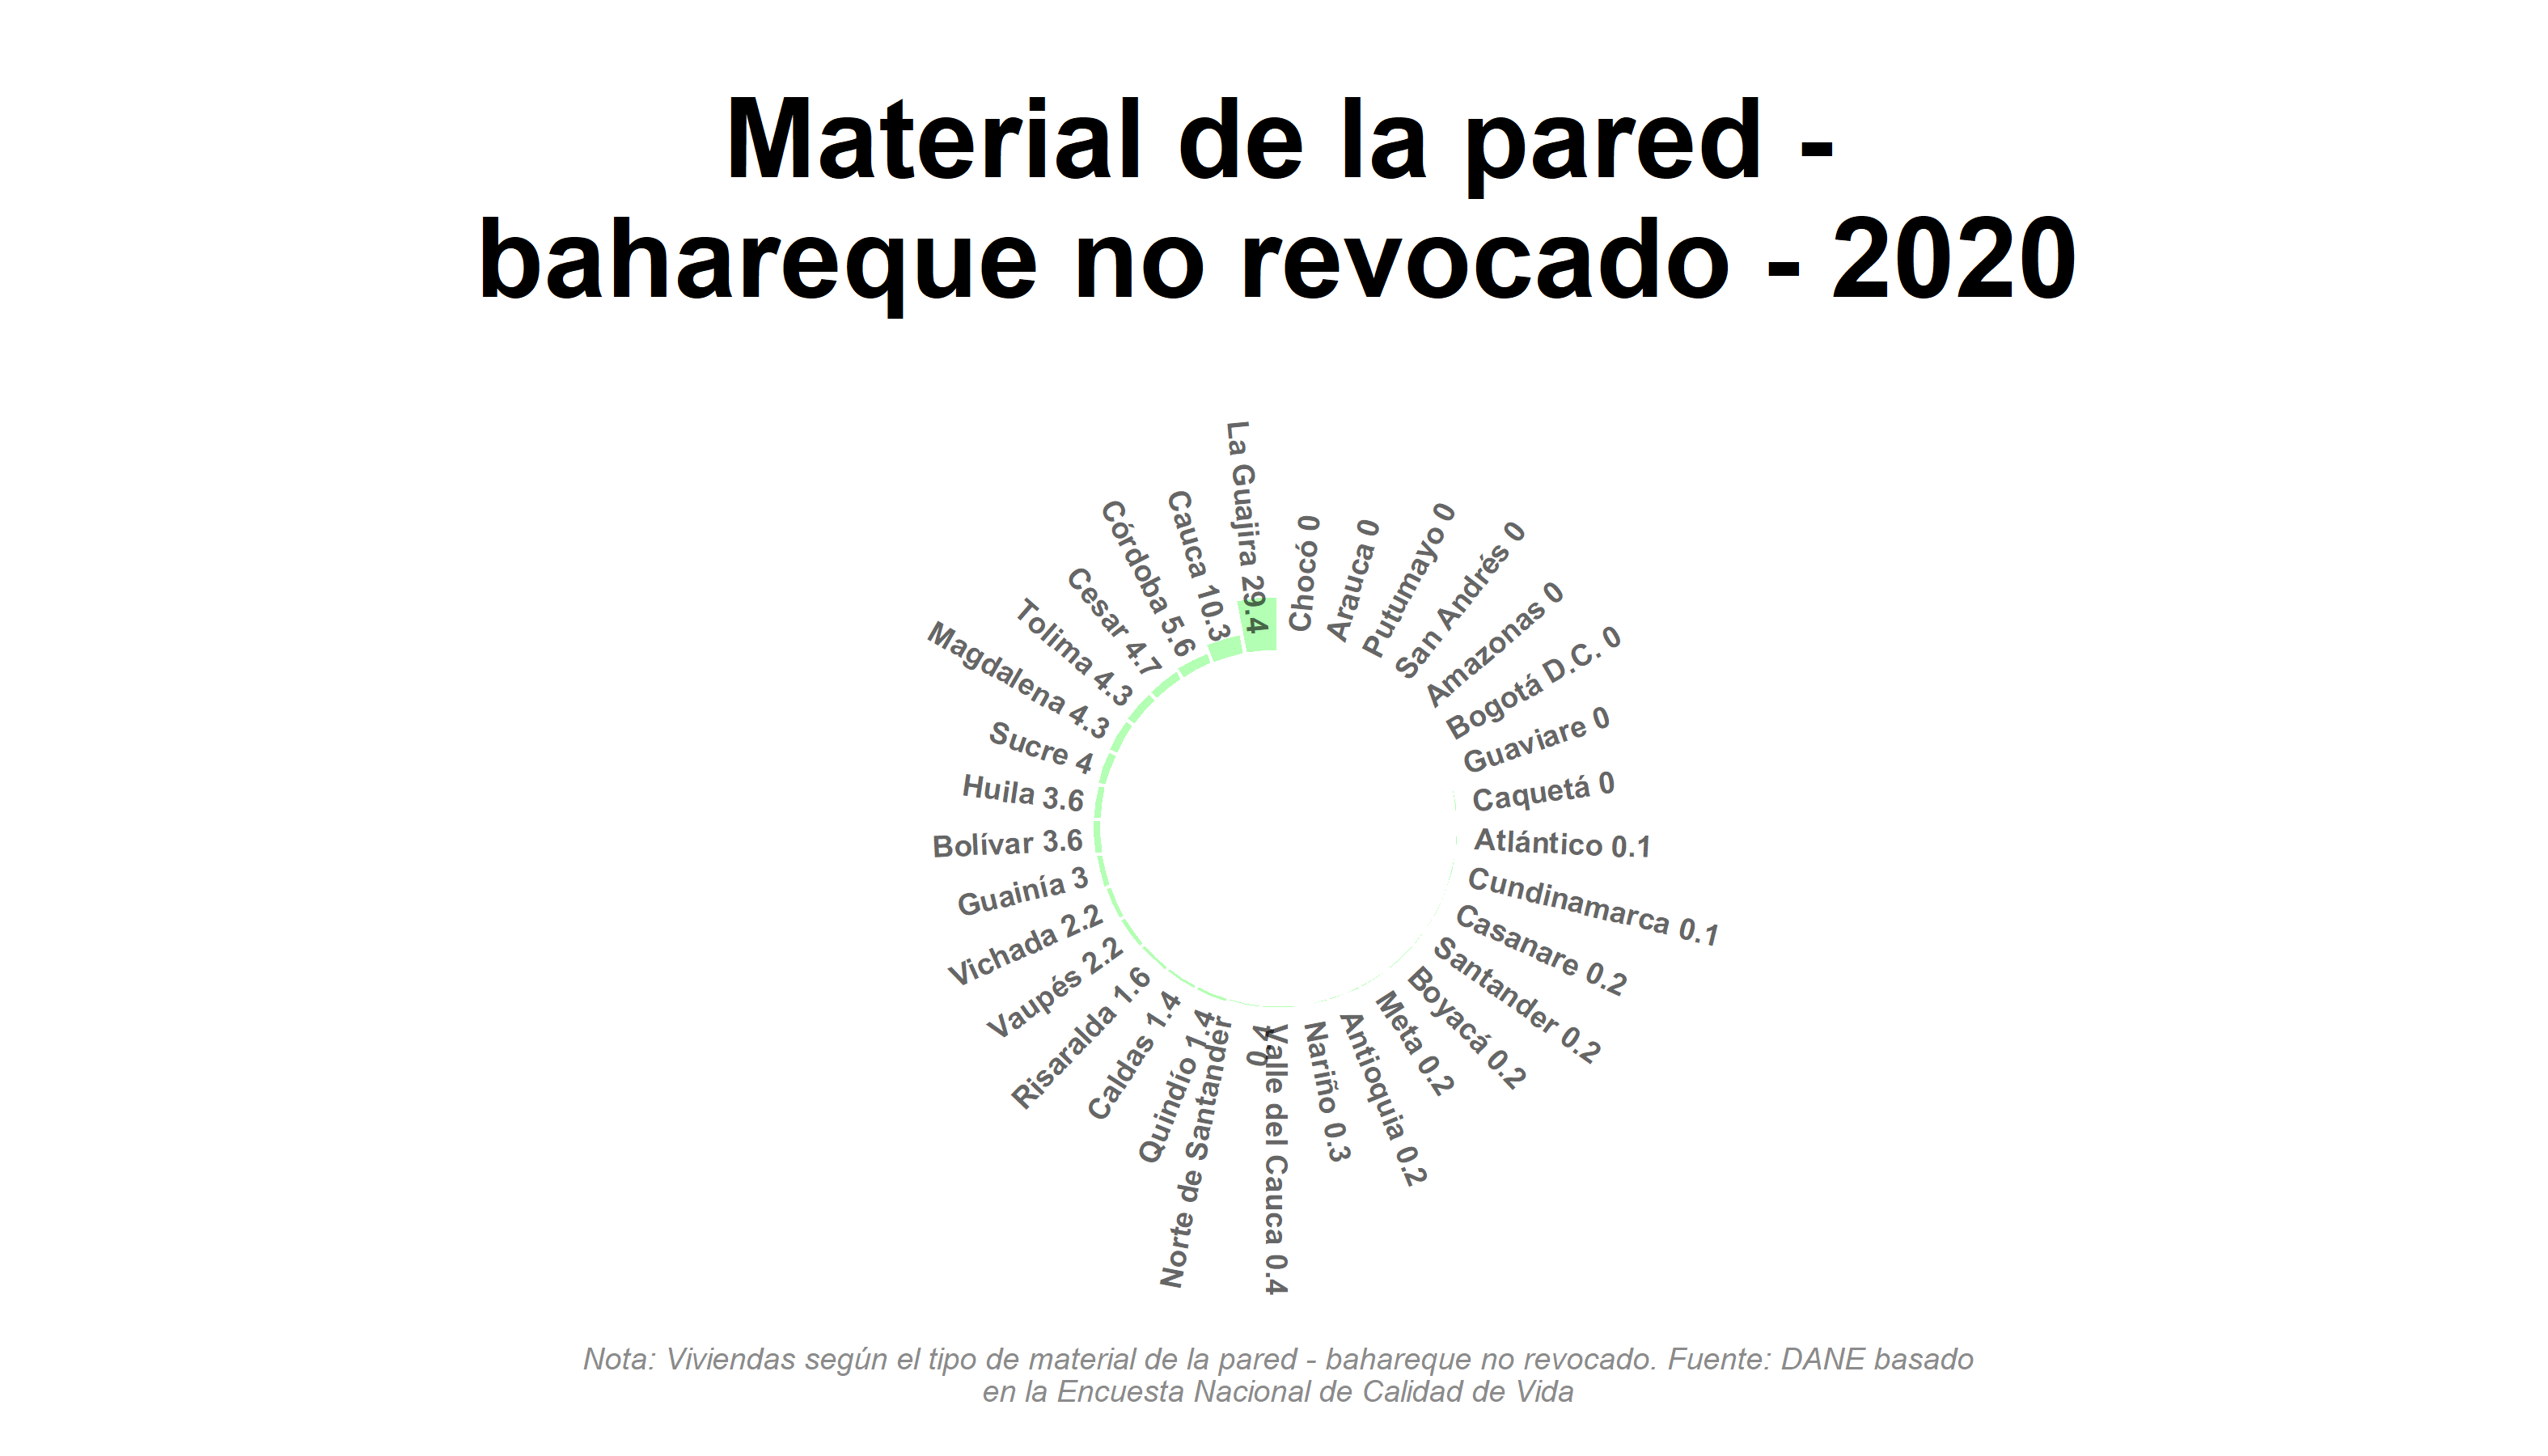
\includegraphics[width=\textwidth,keepaspectratio]{img/var_152_static.png}
        \end{center}
    \end{figure}
            \begin{itemize}
                    \item A pesar de ser el cuarto material más usado solo 2 departamentos superan el 10\% de las viviendas con este material, Cauca y La Guajira.
                    \item Este es el segundo material más usado en La Guajira con un 29.4\%, con una diferencia de cerca del 20\% con el Cauca.
                    \end{itemize}

%%%% Include figures
    \begin{figure}[H]
        \caption{Viviendas con pared de bahareque no revocado por zonas \label{map_result_2} }
        \begin{center}
        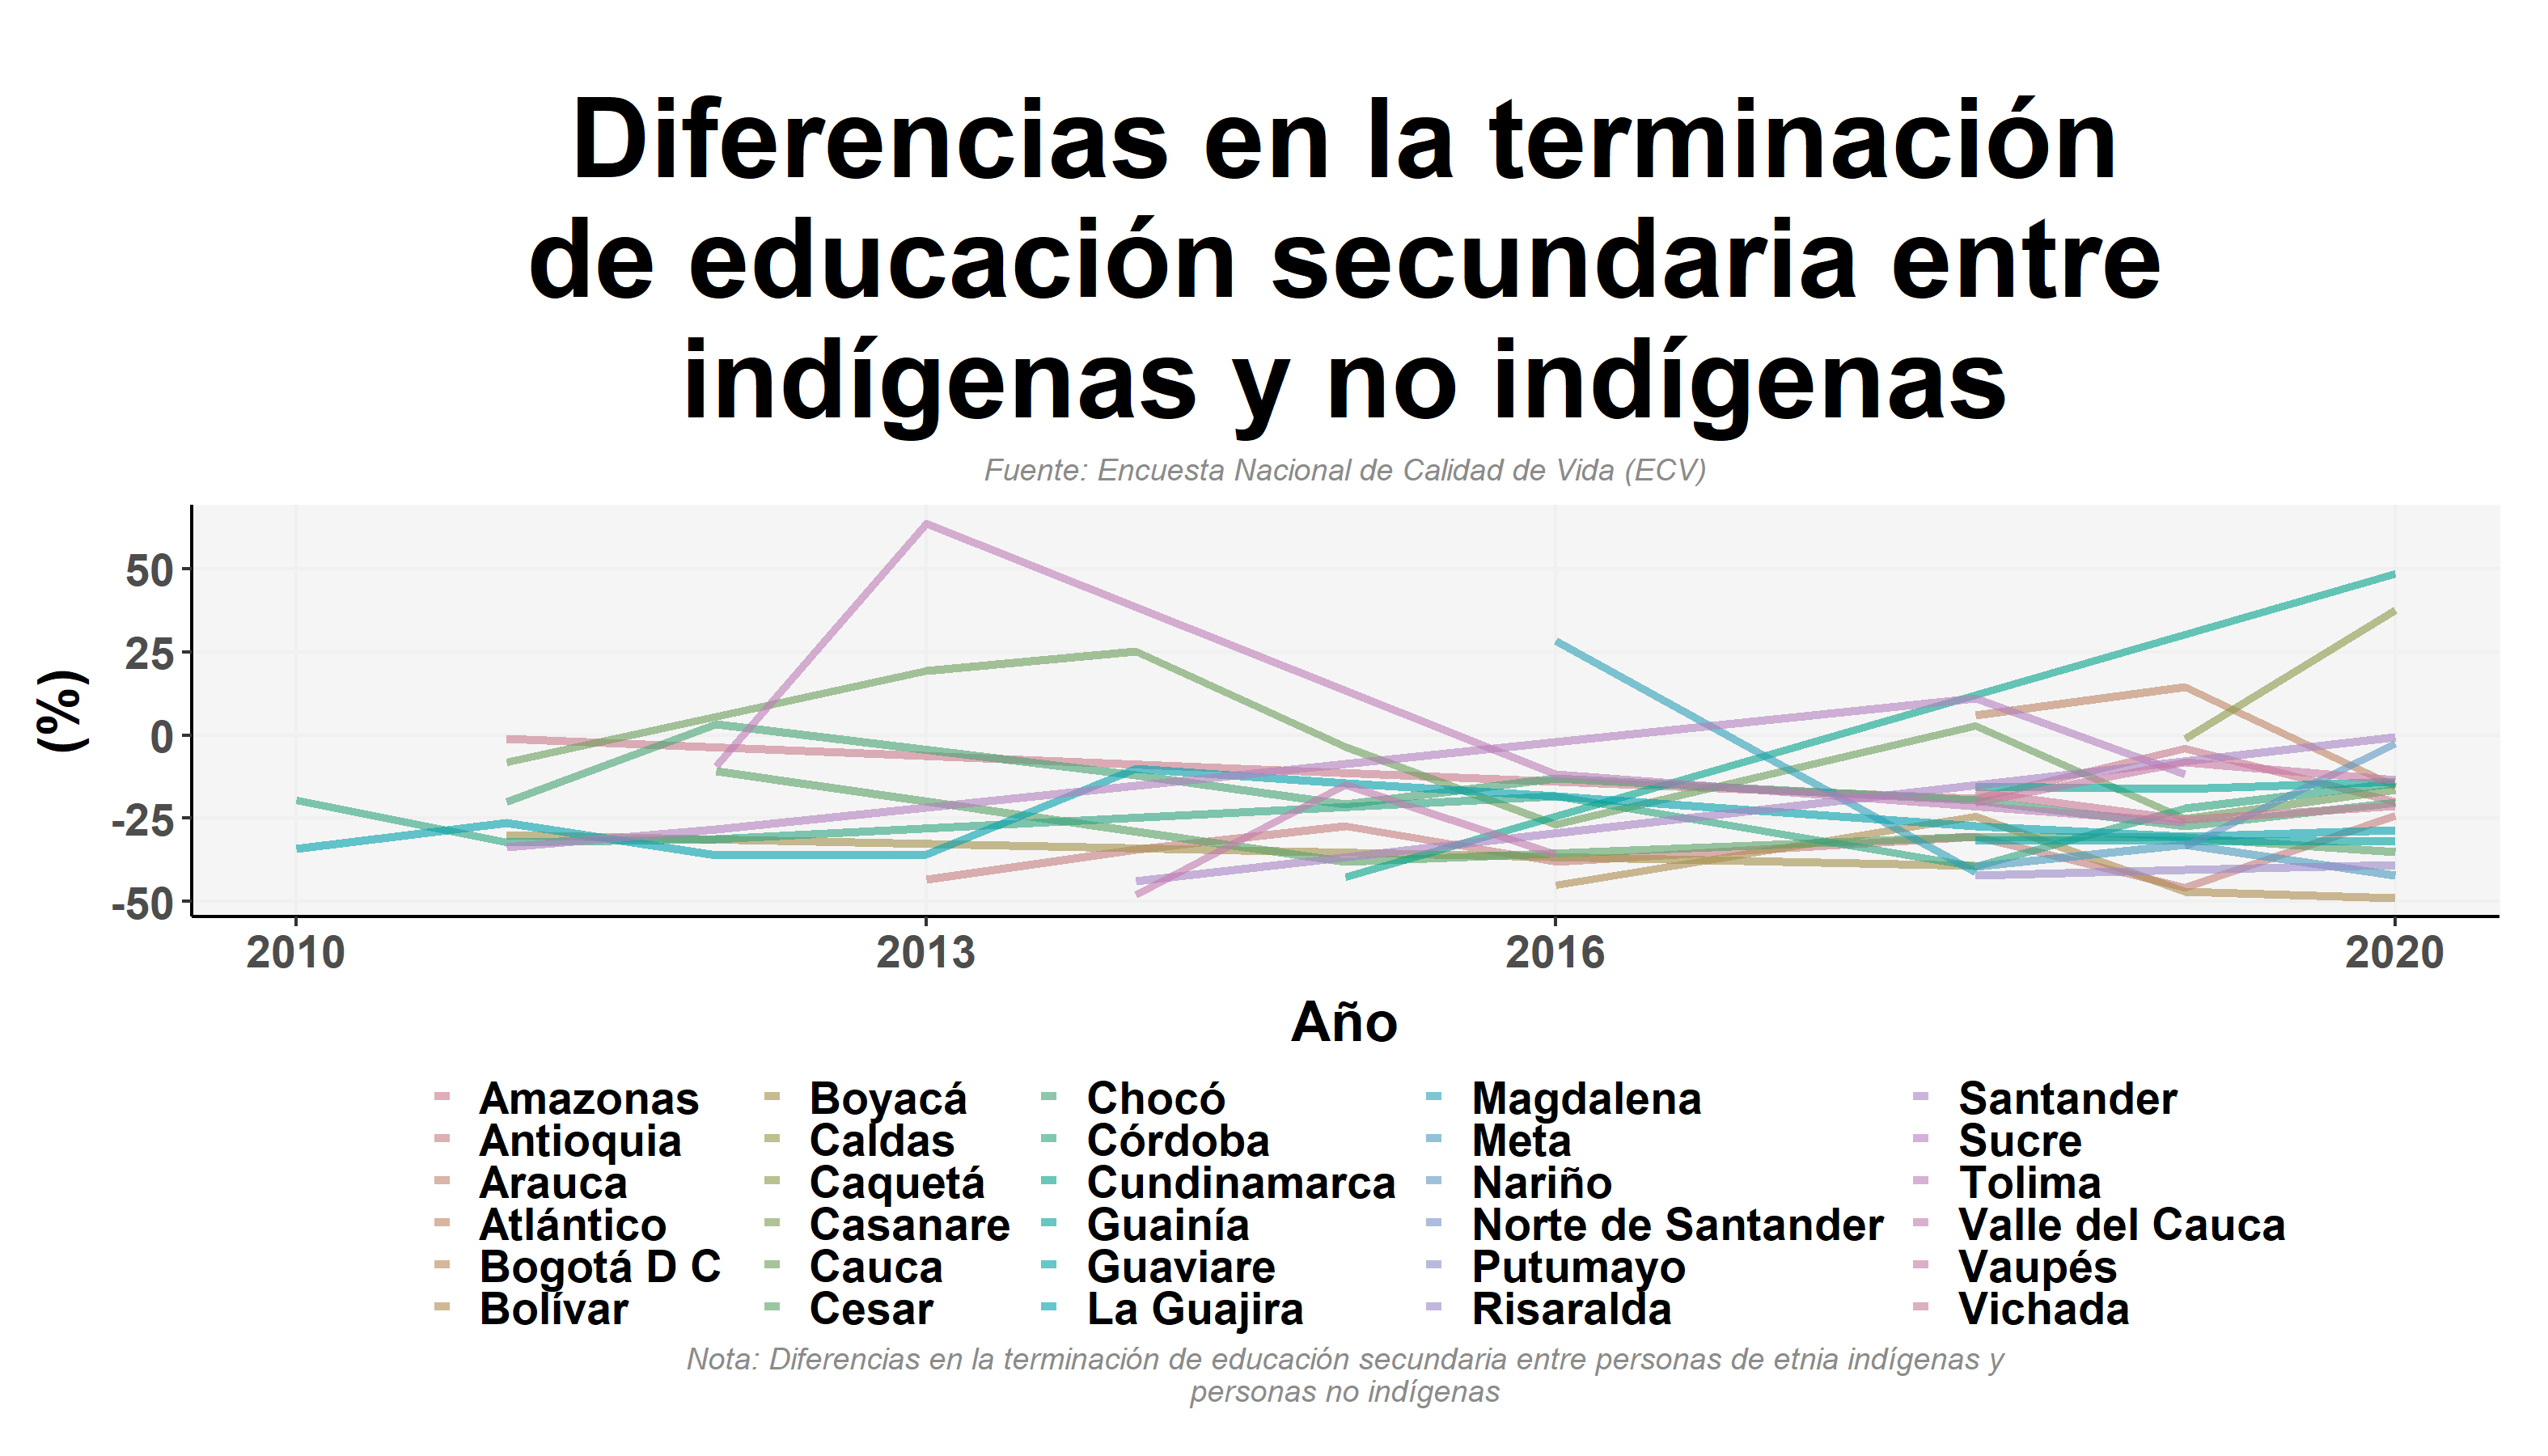
\includegraphics[width=\textwidth,keepaspectratio]{img/var_153_trend.png}
        \end{center}
    \end{figure}
            \begin{itemize}
                    \item Material predominante en las zonas rurales, más del 6\% de las viviendas, en las cabeceras es cercano a cero.
                    \item A pesar que estaba disminuyendo, desde el 2016 tuvo un incremento dejándolo en 2020 con valores cercanos a los niveles del 2010.
                    \end{itemize}

%%%% Include figures
    \begin{figure}[H]
        \caption{Viviendas con pared de latas desechables por departamentos para 2020 \label{map_result_2} }
        \begin{center}
        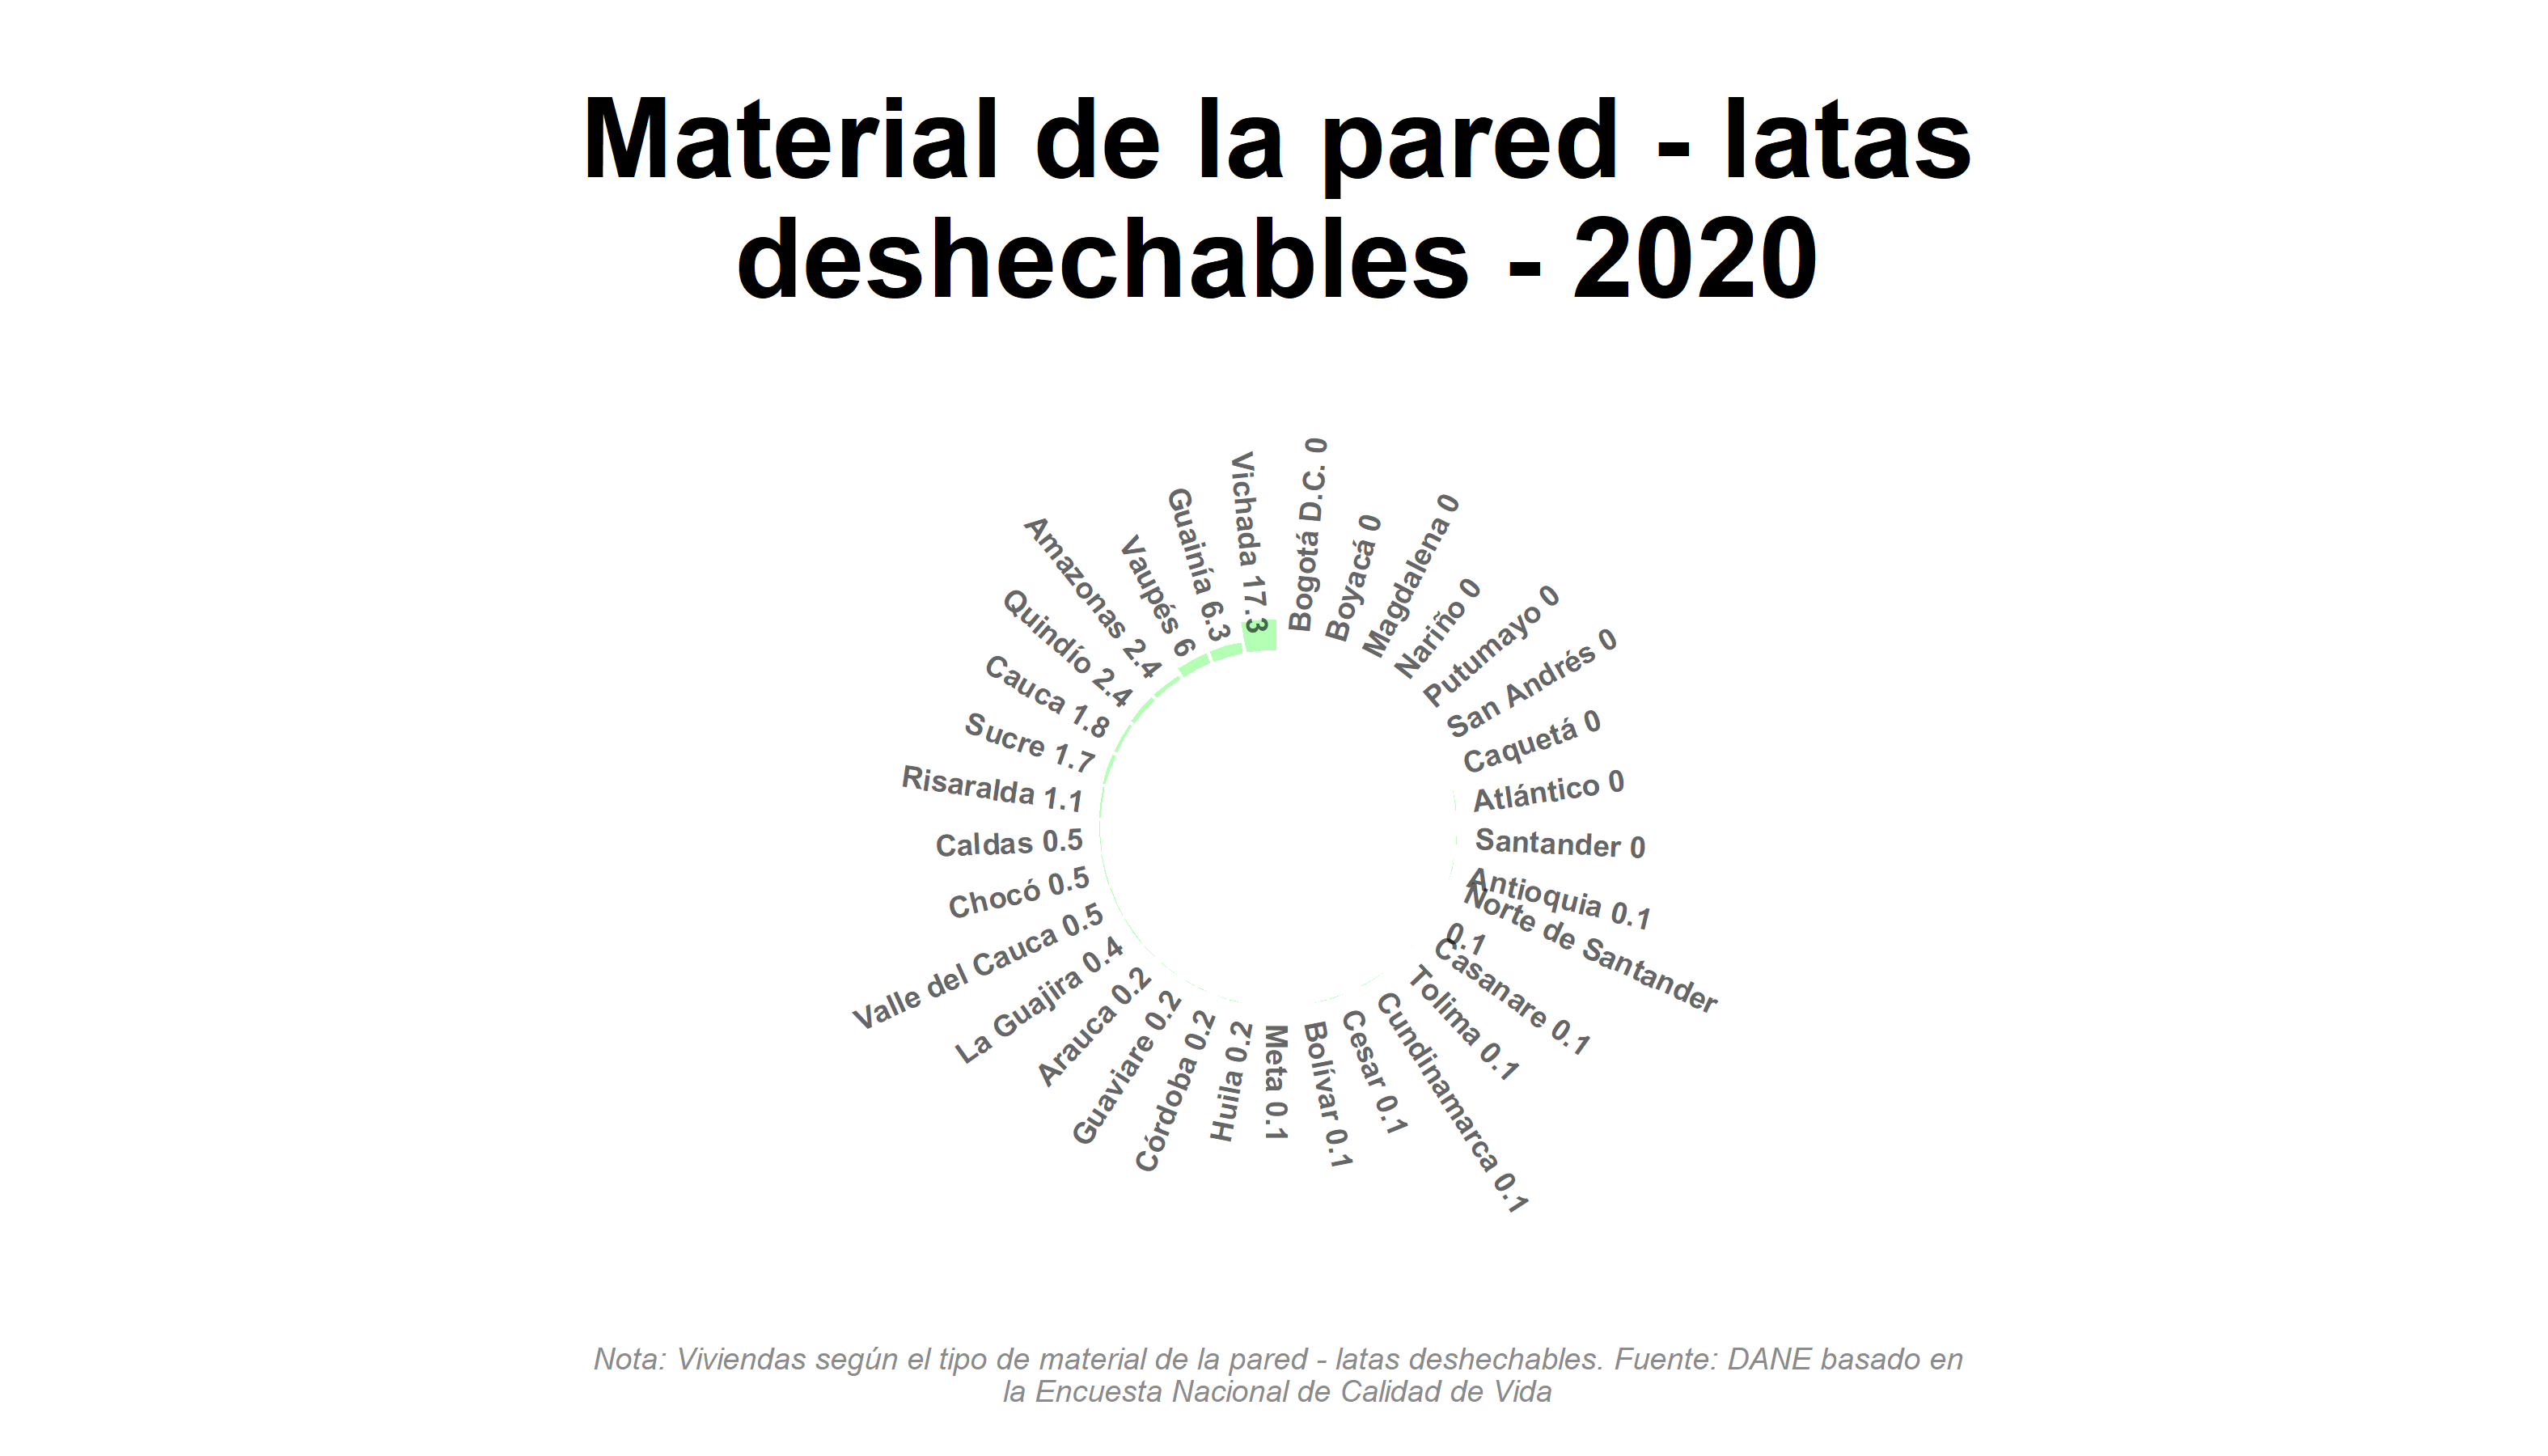
\includegraphics[width=\textwidth,keepaspectratio]{img/var_158_static.png}
        \end{center}
    \end{figure}
            \begin{itemize}
                    \item A pesar de ser uno de los materiales menos usados, se resalta que en Vaupés, Guainía y Vichada es un material bastante usado en comparación.
                    \item En el Vichada es donde más se usa, siendo que el 17.3\% de las viviendas tienen paredes en este material, superando en en poco más del 10\% a Guainía que es el segundo donde más se usa.
                    \end{itemize}

        \subsubsection{Material del Piso}

%%%% Include figures
    \begin{figure}[H]
        \caption{Viviendas con piso de baldosa por departamentos - 2010 VS 2020 \label{map_result_2} }
        \begin{center}
        \includegraphics[width=\textwidth,keepaspectratio]{img/var_173_scatter_time.png}
        \end{center}
    \end{figure}
            \begin{itemize}
                    \item Gran parte de los territorios ha aumentado el porcentaje de viviendas con este material.
                    \item Amazonas y Putumayo son los dptos que tuvieron el mayor retroceso en el porcentaje de viviendas, pasando de estar por el 60\% en 2010 a estar alrededor del 30\% en 2020.
                    \item Cauca, Huila y La Guajira presentan a 2020 niveles similares a los tenidos hace 10 años.
                    \end{itemize}

%%%% Include figures
    \begin{figure}[H]
        \caption{Viviendas con piso de baldosa por departamento para 2020 \label{map_result_2} }
        \begin{center}
        \includegraphics[width=\textwidth,keepaspectratio]{img/var_173_static.png}
        \end{center}
    \end{figure}
            \begin{itemize}
                    \item Más de la mitad de los departamentos tienen menos del 50\% de las viviendas con pisos de baldosa.
                    \item La diferencia entre los territorios extremos es de poco más del 70\% (Bogotá - Vaupés).
                    \item A pesar de ser el material más usado en el piso se denota que la distribución varía mucho entre los territorios yendo desde 6\% hasta el 80\% de las viviendas.
                    \end{itemize}

%%%% Include figures
    \begin{figure}[H]
        \caption{Viviendas con piso de baldosa por zonas \label{map_result_2} }
        \begin{center}
        \includegraphics[width=\textwidth,keepaspectratio]{img/var_174_trend.png}
        \end{center}
    \end{figure}
            \begin{itemize}
                    \item El uso del material para el piso de las viviendas ha aumentado, siendo más significativo en las cabeceras.
                    \item Poco más del 70\% de las viviendas en las cabeceras tienen pisos de baldosa, mientras que en las zonas rurales son el 20\% aproximadamente.
                    \end{itemize}

%%%% Include figures
    \begin{figure}[H]
        \caption{Viviendas con piso de cemento por departamentos - 2010 VS 2020 \label{map_result_2} }
        \begin{center}
        \includegraphics[width=\textwidth,keepaspectratio]{img/var_177_scatter_time.png}
        \end{center}
    \end{figure}
            \begin{itemize}
                    \item Solo Santander, Putumayo y Huila presentan un incremento en el porcentaje de viviendas con pisos de cementos.
                    \item La gran mayoría de los dptos han disminuido las viviendas con este material, estando concentradas por debajo del 45\% para 2020.
                    \item Boyacá mantiene sus niveles de viviendas con pisos de cementos que tenía en el 2010.
                    \end{itemize}

%%%% Include figures
    \begin{figure}[H]
        \caption{Viviendas con piso de cemento por departamentos para 2020 \label{map_result_2} }
        \begin{center}
        \includegraphics[width=\textwidth,keepaspectratio]{img/var_177_static.png}    
        \end{center}
    \end{figure}
            \begin{itemize}
                    \item Más de la mitad de los territorios están por debajo del 40\% de viviendas con piso en cemento.
                    \item El material es el segundo más usado, teniendo una distribución amplia, desde un 6\% hasta un 57\%.
                    \item La diferencia entre los territorios extremos es de aproximadamente un 50\% (Bogotá - Caquetá).
                    \item Los dptos donde el número de viviendas con este tipo de material es mayor se encuentran especialmente en la costa, en zonas de frontera o al sur del país. Los territorios en el centro tienden a reportar menores niveles.
                    \end{itemize}

%%%% Include figures
    \begin{figure}[H]
        \caption{Viviendas con piso de cemento por zonas \label{map_result_2} }
        \begin{center}
        \includegraphics[width=\textwidth,keepaspectratio]{img/var_178_trend.png}
        \end{center}
    \end{figure}
            \begin{itemize}
                    \item En general se puede ver que en ambas zonas hay una disminución de las viviendas con piso de cemento.
                    \item El uso de cemento como material para el piso es predominante en las zonas rurales, poco más del 50\% para 2020, mientras que en las cabeceras está cercano al 20\% de las viviendas.
                    \end{itemize}

%%%% Include figures
    \begin{figure}[H]
        \caption{Viviendas con piso de tierra por departamentos - 2010 VS 2020 \label{map_result_2} }
        \begin{center}
        \includegraphics[width=\textwidth,keepaspectratio]{img/var_179_scatter_time.png}
        \end{center}
    \end{figure}
            \begin{itemize}
                    \item Se denota como gran parte de los departamentos están concentrados en valores inferiores al 10\% y mantenidos entre los dos años de referencia. 
                    \item La Guajira y Arauca destacan al presentar el doble de viviendas con piso de tierra en 2020 comparada con las del 2010.
                    \item Por el lado de Córdoba y Magdalena se ve como han disminución notable en cuanto a viviendas con pisos de tierra.
                    \end{itemize}

%%%% Include figures
    \begin{figure}[H]
        \caption{Viviendas con piso de tierra por departamentos para 2020 \label{map_result_2} }
        \begin{center}
        \includegraphics[width=\textwidth,keepaspectratio]{img/var_179_static.png}
        \end{center}
    \end{figure}
            \begin{itemize}
                    \item Los extremos entre el de menor y mayor porcentaje de viviendas es avismal, teniendo a San Andrés con el 0.3\% de viviendas con piso de tierra, mientras que en el Vichada son el 66.4\% de estas, es decir que más de la mitad de las viviendas están en esta condición.
                    \item Más de la mitad de los dptos están por debajo del 10\%.
                    \item Los dptos con mayor nivel de viviendas con este tipo de piso se encuentran principalmente en la costa Caribe y en el oriente, mientras que los de menor están en la zona cafetera (gráfica map 179 para 2020).
                    \end{itemize}

%%%% Include figures
    \begin{figure}[H]
        \caption{Viviendas con piso de tierra por zonas \label{map_result_2} }
        \begin{center}
        \includegraphics[width=\textwidth,keepaspectratio]{img/var_180_trend.png}
        \end{center}
    \end{figure}
            \begin{itemize}
                    \item En las zonas rurales los pisos de tierra se presentan alrededor en el 20\% de las viviendas, mientras que en las cabeceras es menos del 3\%.
                    \item En las zonas rurales a pesar de que a principios de la década estaban disminuyendo las viviendas con este tipo de piso, desde el 2015 esta ha venido aumentan, teniendo para 2020 niveles superiores a los reportados en 2010.
                    \item Para las cabeceras las viviendas con este tipo de material han disminuido, pero aun se mantienen cerca al mismo nivel que hace 10 años.
                    \end{itemize}

%%%% Include figures
    \begin{figure}[H]
        \caption{Viviendas con piso de madera burda por departamentos - 2010 VS 2020 \label{map_result_2} }
        \begin{center}
        \includegraphics[width=\textwidth,keepaspectratio]{img/var_175_scatter_time.png}
        \end{center}
    \end{figure}
            \begin{itemize}
                    \item La mayoría de los dptos se encuentran concentrados en cero o cerca a este.
                    \item Amazonas y Chocó son los departamentos que más aumentaron las viviendas con este tipo de pisos, triplicando y doblando, respectivamente, los valores presentados en 2010.
                    \item Caquetá y Caldas tuvieron las mayores mejoras, siendo la primera la mitad de lo que presentó en 2010.
                    \item Nariño mantiene los niveles que tenía hace 10 años.
                    \end{itemize}

%%%% Include figures
    \begin{figure}[H]
        \caption{Viviendas con piso de madera burda por departamentos para 2020 \label{map_result_2} }
        \begin{center}
        \includegraphics[width=\textwidth,keepaspectratio]{img/var_175_static.png}
        \end{center}
    \end{figure}
            \begin{itemize}
                    \item Solo 6 dptos presentan más del 10\% de las viviendas con pisos de este material.
                    \item Los últimos 3 dptos tienen valores alrededor del 40\%, Vaupés, Chocó y Amazonas.
                    \item Amazonas tiene casi la mitad de las viviendas con piso de madera burda, siendo este el dpto con más porcentaje, mientras que La Guajira presenta el 0.2\% de las viviendas con pisos de este material.
                    \end{itemize}

%%%% Include figures
    \begin{figure}[H]
        \caption{Viviendas con piso de madera burda por zonas \label{map_result_2} }
        \begin{center}
        \includegraphics[width=\textwidth,keepaspectratio]{img/var_176_trend.png}
        \end{center}
    \end{figure}
            \begin{itemize}
                    \item Para las cabeceras se ha mantenido el porcentaje de viviendas con este tipo de piso en alrededor del 2\%, con una leve disminución en el tiempo.
                    \item Para la zona rural el porcentaje de viviendas se mantuvo constante la primera mitad de la década, pero después del 2016 aumentó, mostrando para 2020 niveles superiores a los registrados en 2012.
                    \end{itemize}

        \subsubsection{Hacinamiento}

%%%% Include figures
    \begin{figure}[H]
        \caption{Hacinamiento por departamentos - Cambio porcentual entre 2018 y 2020 \label{map_result_2} }
        \begin{center}
        \includegraphics[width=\textwidth,keepaspectratio]{img/var_265_map_change.png}
        \end{center}
    \end{figure}
            \begin{itemize}
                    \item Los dptos de Chocó, Putumayo, Córdoba, Bolívar, Boyacá, Guainía y Meta presentaron una disminución del hacinamiento crítico de más del 20\%.
                    \item Por otro lado Quindío, Tolima, Huila, Bogotá, Guaviare y Vaupés fueron lo que más aumentaron los niveles de hacinamiento crítico.
                    \end{itemize}

%%%% Include figures
    \begin{figure}[H]
        \caption{Hacinamiento por departamentos para 2020 \label{map_result_2} }
        \begin{center}
        \includegraphics[width=\textwidth,keepaspectratio]{img/var_265_static.png}
        \end{center}
    \end{figure}
            \begin{itemize}
                    \item La distribución de los valores va desde 3\% hasta poco más del 30\%.
                    \item Los territorios con mayor hacinamiento crítico se ubican en la zona Caribe y el oriente - Amazonia (gráfica mas 265 para 2020).
                    \item Más de la mitad de los dptos tiene niveles por debajo del 10\% de hacinamiento crítico.
                    \item La diferencia entre el territorio con menor y mayor para 2020 nivel de hacinamiento es de cerca al 30\% (Boyacá - Vaupés).
                    \end{itemize}

%%%% Include figures
    \begin{figure}[H]
        \caption{Hacinamiento por zonas y nacional \label{map_result_2} }
        \begin{center}
        \includegraphics[width=\textwidth,keepaspectratio]{img/var_267_trend.png}
        \end{center}
    \end{figure}
            \begin{itemize}
                    \item Tanto las zonas como a nivel nacional hay una tendencia a la baja en el hacinamiento crítico, teniendo menores niveles para 2020 comparados con los reportados en 2010.
                    \item Para 2019 se ve un pico pronunciado en las cabeceras y a nivel nacional, pero en las zonas rurales este siguió a la baja en ese año.
                    \item La brecha entre las zonas rurales y cabeceras a pesar de haber disminuido, siendo el hacinamiento menor en las zonas rurales, a partir del 2019 aumentó significativamente, llevando a tener la brecha similar al 2013, un retroceso de 7 años.
                    \end{itemize}

\section{Acceso a servicios de agua potable y saneamiento}
    \subsection{Agua Potable}

%%%% Include figures
    \begin{figure}[H]
        \caption{Acueducto público como fuentes de agua por departamentos - 2010 VS 2020 \label{map_result_2} }
        \begin{center}
        \includegraphics[width=\textwidth,keepaspectratio]{img/var_129_scatter_time.png}
        \end{center}
    \end{figure}
            \begin{itemize}
                    \item Es la fuente de agua más común en el país, siendo para la mayoría de los dptos más del 50\% de las viviendas usan esta fuente.
                    \item En general para 2020 la mayoría de los dptos han mejorado o mantenido los niveles que presentaron en 2010.
                    \item Chocó es el que presenta el mayor cambio entre lo años, pasando de que más del 60\% de las viviendas tengan esta fuente de agua en 2010, a manos del 25\% de las viviendas en el 2020.
                    \end{itemize}

%%%% Include figures
    \begin{figure}[H]
        \caption{Acueducto público como fuentes de agua por departamentos para 2020 \label{map_result_2} }
        \begin{center}
        \includegraphics[width=\textwidth,keepaspectratio]{img/var_129_static.png}
        \end{center}
    \end{figure}
            \begin{itemize}
                    \item Aunque más de la mitad de los territorios tienen como fuente de agua el acueducto público en más del 60\% de las viviendas, también hay zonas con menos del 20\%.
                    \item Bogotá es el territorio con más viviendas con esta fuente de agua, 98.9\%, mientras que Vaupés presenta el menor número con un 0.8\%.
                    \item Las zonas de menor acceso a esta fuente de agua se encuentran ubicadas en la región de la Amazonia y los llanos orientales, y el Chocó (map 129 2020).
                    \end{itemize}

%%%% Include figures
    \begin{figure}[H]
        \caption{Acueducto público como fuentes de agua por zonas \label{map_result_2} }
        \begin{center}
        \includegraphics[width=\textwidth,keepaspectratio]{img/var_130_trend.png}
        \end{center}
    \end{figure}
            \begin{itemize}
                    \item Mientras que en las cabeceras más del 90\% de las viviendas tienen acceso a un acueducto público, en las zonas rurales es cerca del 20\%.
                    \item En el trascurso de los años el porcentaje de viviendas con acceso a un acueducto público se ha mantenido en valores similares, sin mayores cambios desde el 2010.
                    \end{itemize}

%%%% Include figures
    \begin{figure}[H]
        \caption{Acueducto comunal como fuentes de agua por departamentos - 2010 VS 2020 \label{map_result_2} }
        \begin{center}
        \includegraphics[width=\textwidth,keepaspectratio]{img/var_133_scatter_time.png}
        \end{center}
    \end{figure}
            \begin{itemize}
                    \item Aunque en la mayoría de los dptos ha aumentado las viviendas con el acceso a esta fuente de agua, gran parte se concentra por debajo del 20\%.
                    \item Meta, Nariño, Risaralda y Caldas son los dptos donde más disminuyó el acceso a esta fuente de agua entre los años de referencia.
                    \end{itemize}

%%%% Include figures
    \begin{figure}[H]
        \caption{Acueducto comunal como fuentes de agua por departamentos para 2020 \label{map_result_2} }
        \begin{center}
        \includegraphics[width=\textwidth,keepaspectratio]{img/var_133_static.png}
        \end{center}
    \end{figure}
            \begin{itemize}
                    \item Se encuentra que para 2020 el 75\% de los territorios tienen menos del 15\% de las viviendas con acceso a un acueducto comunal.
                    \item Hay territorio que no tienen acueducto comunal, San Andrés y Vaupés, siendo los de menor rango, mientras que Boyacá, Nariño y Cauca tienen alrededor de un 30\% de las viviendas que dependen de esta fuente de agua, siendo el de mayor porcentaje Cauca con un 34.5\%.
                    \item Esta fuente de agua se concentra en el 2020 en la zona centro y sur-occidente del país (map 133 2020)
                    \end{itemize}

%%%% Include figures
    \begin{figure}[H]
        \caption{Acueducto comunal como fuentes de agua por zonas \label{map_result_2} }
        \begin{center}
        \includegraphics[width=\textwidth,keepaspectratio]{img/var_134_trend.png}
        \end{center}
    \end{figure}
            \begin{itemize}
                    \item El acueducto tiene un papel protagónico en los centros poblados y rural disperso, siendo la fuente de agua para cerca del 40\% de las viviendas, mientras que en las cabeceras son menos del 5\% de las viviendas.
                    \item Para la zona rural vemos que ha sido muy variada en los años, y aunque a finales de la década estaba disminuyendo, para 2020 aumentó superando los valores del 2010.
                    \end{itemize}

%%%% Include figures
    \begin{figure}[H]
        \caption{Río o quebradas como fuentes de agua por departamentos - 2010 VS 2020 \label{map_result_2} }
        \begin{center}
        \includegraphics[width=\textwidth,keepaspectratio]{img/var_142_scatter_time.png}
        \end{center}
    \end{figure}
            \begin{itemize}
                    \item Es la tercera fuente de agua más usada por las viviendas aunque gran parte de los territorios está concentrada por debajo del 10\% y la mayoría tuvieron mejoras entre el 2010 y 2020.
                    \item Algunos dptos no están dado que se tuvieron en cuenta en la ECV desde 2018.
                    \end{itemize}

%%%% Include figures
    \begin{figure}[H]
        \caption{Río o quebradas como fuentes de agua por departamentos para 2020 \label{map_result_2} }
        \begin{center}
        \includegraphics[width=\textwidth,keepaspectratio]{img/var_141_static.png}
        \end{center}
    \end{figure}
            \begin{itemize}
                    \item Todos los dptos están por debajo del 20\%, incluso más del 75\% de estos están por debajo del 10\%, pero hay uno que es el de mayor porcentaje, Vichada, donde cerca del 60\% de las viviendas su fuente de agua es un río o una quebrada.
                    \item Los dptos que más usan esta fuente de agua se encuentran principalmente en la zona oriental y amazónica (map 141 2020)
                    \end{itemize}

%%%% Include figures
    \begin{figure}[H]
        \caption{Río o quebradas como fuentes de agua por zonas \label{map_result_2} }
        \begin{center}
        \includegraphics[width=\textwidth,keepaspectratio]{img/var_142_trend.png}
        \end{center}
    \end{figure}
            \begin{itemize}
                    \item Es principalmente usada en las zonas rurales, alrededor del 15\%.
                    \item Para las cabeceras el uso de esta fuente agua es cercano a cero.
                    \item En los últimos años a disminuido el uso de esta fuente de en la zona rural, mostrando valores menores en 2020 a los registrados en el 2010.
                    \end{itemize}

%%%% Include figures
    \begin{figure}[H]
        \caption{Pozo con bomba como fuentes de agua por departamentos - 2010 VS 2020 \label{map_result_2} }
        \begin{center}
        \includegraphics[width=\textwidth,keepaspectratio]{img/var_135_scatter_time.png}
        \end{center}
    \end{figure}
            \begin{itemize}
                    \item Aunque en la mayoría de los dptos no es una fuente de agua muy utilizada, tenemos casos como Casanare y Arauca que pasaron de 0\% de viviendas con esta fuente, a más del 10\%, incluso del 20\% para Arauca.
                    \item En zonas como Amazonas, Bolívar, Putumayo y Magdalena el porcentaje de viviendas con esta fuente de agua disminuyó.
                    \end{itemize}

%%%% Include figures
    \begin{figure}[H]
        \caption{Pozo con bomba como fuentes de agua por departamentos para 2020 \label{map_result_2} }
        \begin{center}
        \includegraphics[width=\textwidth,keepaspectratio]{img/var_135_static.png}
        \end{center}
    \end{figure}
            \begin{itemize}
                    \item Menos del 10\% de las viviendas en el 75\% de los territorios usan el pozo con bomba como fuente de agua.
                    \item Los últimos cuatro dptos tienen por encima del 20\% de las viviendas con esta fuente de agua. Se destaca que los dptos hacen parte de la zona oriental y amazónica del país, donde es popular esta fuente de agua (map 135 2020).
                    \item Guainía es el dpto con mayor proporción de viviendas con esta fuente de agua, 37.1\%, mientras que Bogotá presenta el menor, con cero viviendas, seguido por Caldas con el 0.1\%.
                    \end{itemize}

%%%% Include figures
    \begin{figure}[H]
        \caption{Pozo con bomba como fuentes de agua por zonas \label{map_result_2} }
        \begin{center}
        \includegraphics[width=\textwidth,keepaspectratio]{img/var_136_trend.png}
        \end{center}
    \end{figure}
            \begin{itemize}
                    \item Es una fuente de agua utilizada especialmente en la zona rural que ha venido en aumento presentando para 2020 valores superiores a los del 2010, aunque en el 2020 hubo una disminución de este.
                    \item Para la cabeceras estás son menos del 1 \%. de las viviendas y se ha mantenido constante.
                    \end{itemize}

%%%% Include figures
    \begin{figure}[H]
        \caption{Agua lluvia como fuentes de agua por departamentos - 2010 VS 2020 \label{map_result_2} }
        \begin{center}
        \includegraphics[width=\textwidth,keepaspectratio]{img/var_139_scatter_time.png}
        \end{center}
    \end{figure}
            \begin{itemize}
                    \item Es una fuente de agua poco común donde la mayoría de los territorios menos del 5\% de las viviendas la usas, pero en territorios como Chocó se duplicó aproximadamente las viviendas que usan esta fuente de agua, o el Amazonas donde pasó de reportar niveles cercanos a cero en 2010 a más del 30\% en el 2020.
                    \item Córdoba pasó de tener poco más del 30\% de las viviendas teniendo como fuente de agua la lluvia en 2010 a niveles cercanos a cero en el 2020, Putumayo y Magdalena también presentaron cambios similares.
                    \end{itemize}

%%%% Include figures
    \begin{figure}[H]
        \caption{Agua lluvia como fuentes de agua por departamentos para 2020 \label{map_result_2} }
        \begin{center}
        \includegraphics[width=\textwidth,keepaspectratio]{img/var_139_static.png}
        \end{center}
    \end{figure}
            \begin{itemize}
                    \item Más del 75\% de los territorios tienen menos del 10\% de las viviendas con el agua lluvia como fuente de agua.
                    \item Vaupés y Chocó son los dptos con mayor viviendas con esta fuente de agua, siendo el 84.6\% y 70.4\% de las viviendas respectivamente, a esto también se le unen dptos como Amazonas y Guainía pero con valores entre 20 y 30\% aproximadamente.
                    \item Los dptos con mayor uso de esta fuente de agua se encuentran en el sur y occidente del país (map 139 2020).
                    \end{itemize}

%%%% Include figures
    \begin{figure}[H]
        \caption{Agua lluvia como fuentes de agua por zonas \label{map_result_2} }
        \begin{center}
        \includegraphics[width=\textwidth,keepaspectratio]{img/var_140_trend.png}
        \end{center}
    \end{figure}
            \begin{itemize}
                    \item Es una fuente de agua especialmente usada en las zonas rurales, estando alrededor del 6\% de las viviendas.
                    \item Para las cabeceras esta ha estado disminuyendo hasta niveles por debajo del 1\%.
                    \item En ambas zonas se registraron valores menores en 2020 comparados con los de 2010.
                    \end{itemize}

%%%% Include figures
    \begin{figure}[H]
        \caption{Pozo sin bomba como fuentes de agua por departamentos para 2020 \label{map_result_2} }
        \begin{center}
        \includegraphics[width=\textwidth,keepaspectratio]{img/var_137_static.png}
        \end{center}
    \end{figure}
            \begin{itemize}
                    \item Se resalta que para La Guajira y Putumayo el 30.2\% y el 21.9\% de las viviendas respectivamente usan el pozo sin bomba como fuente de agua.
                    \item Para los demás dptos, poco más del 75\% de ellos, son menos del 5\% de las viviendas lo usan como fuente de agua.
                    \end{itemize}

%%%% Include figures
    \begin{figure}[H]
        \caption{Agua en botella o bolsa como fuentes de agua por departamentos para 2020 \label{map_result_2} }
        \begin{center}
        \includegraphics[width=\textwidth,keepaspectratio]{img/var_143_static.png}
        \end{center}
    \end{figure}
            \begin{itemize}
                    \item Para San Andrés el agua en botella o en bolsa es una de las principales fuentes de agua, siendo esta para el 41.1\% de las viviendas en el dpto. Vaupés le sigue con el 12.3\% de las viviendas.
                    \item A excepción de los dptos mencionados anteriormente los demás territorios están por debajo del 10\%, incluso la mayoría está por debajo del 3\%.
                    \end{itemize}

%%%% Include figures
    \begin{figure}[H]
        \caption{Carrotanque como fuentes de agua por departamentos para 2020 \label{map_result_2} }
        \begin{center}
        \includegraphics[width=\textwidth,keepaspectratio]{img/var_147_static.png}
        \end{center}
    \end{figure}
            \begin{itemize}
                    \item Es de las fuentes de agua menos común en el país, donde cerca del 80\% son menos del 1\%, pero se destaca que en La Guajira el 10.4\% de las viviendas tienen como fuente de agua el carrotanque.
                    \end{itemize}

    \subsection{Saneamiento}

%%%% Include figures
    \begin{figure}[H]
        \caption{Saneamiento dentro de la vivienda por departamentos - 2010 VS 2020 \label{map_result_2} }
        \begin{center}
        \includegraphics[width=\textwidth,keepaspectratio]{img/var_193_scatter_time.png}
        \end{center}
    \end{figure}
            \begin{itemize}
                    \item Gran parte de los territorios están concentrados por encima del 75\% de las viviendas, además de que en general el saneamiento al interior de las viviendas ha aumentado entre 2010 y 2020.
                    \item Arauca, Putumayo y Amazonas muestran un gran retroceso en el porcentaje de viviendas con el saneamiento en el interior, pasando de valores cercanos al 80\% en 2010 a cerca del 50\% en el 2020.
                    \item Huila, Tolima y Nariño mantuvieron los niveles que tenían hace 10 años.
                    \end{itemize}

%%%% Include figures
    \begin{figure}[H]
        \caption{Saneamiento dentro de la vivienda por departamentos (mapa) - 2010 VS 2020 \label{map_result_2} }
        \begin{center}
        \includegraphics[width=\textwidth,keepaspectratio]{img/var_193_map.png}
        \end{center}
    \end{figure}
            \begin{itemize}
                    \item Se ve que en el centro del país para 2020 se aumenta el porcentaje de viviendas con baño en el interior, caso contrario pasa a medida que se aleja del centro. 
                    \item Se destaca que la zonas del oriente y la Amazonia se centran los territorios con menor porcentaje de viviendas con saneamiento en el interior.
                    \end{itemize}

%%%% Include figures
    \begin{figure}[H]
        \caption{Saneamiento dentro de la vivienda por departamentos para 2020 \label{map_result_2} }
        \begin{center}
        \includegraphics[width=\textwidth,keepaspectratio]{img/var_193_static.png}
        \end{center}
    \end{figure}
            \begin{itemize}
                    \item Los 3 departamentos que menos tienen viviendas con saneamiento dentro están por debajo del 30\%, mientras que más de la mitad de los territorios está por encima del 65\% de las viviendas.
                    \item Mientras que en Vaupés solo 17.9\% de las viviendas tienen el saneamiento en el interior, en Bogotá es el 98.7\% de las viviendas.
                    \end{itemize}

%%%% Include figures
    \begin{figure}[H]
        \caption{Saneamiento dentro de la vivienda por zonas \label{map_result_2} }
        \begin{center}
        \includegraphics[width=\textwidth,keepaspectratio]{img/var_194_trend.png}
        \end{center}
    \end{figure}
            \begin{itemize}
                    \item En ambas zonas han aumentado las viviendas con el saneamiento en el interior, siendo este mayor en las zonas rurales.
                    \item La zona rural presenta un aumento, logrando que la zona rural pase del 50\% de las viviendas con saneamiento en el interior.
                    \end{itemize}

%%%% Include figures
    \begin{figure}[H]
        \caption{Saneamiento fuera de la vivienda por departamentos - 2010 VS 2020 \label{map_result_2} }
        \begin{center}
        \includegraphics[width=\textwidth,keepaspectratio]{img/var_195_scatter_time.png}
        \end{center}
    \end{figure}
            \begin{itemize}
                    \item En la mayoría de los dptos se ha disminuido las viviendas con saneamiento fuera, especialmente en el Meta, La Guajira, Cundinamarca y Casanare.
                    \item Huila y Bogotá presentan a 2020 los mismos niveles que en el 2010.
                    \item Arauca, Amazonas, Putumayo y Norte son los dptos que tuvieron un aumento significativo en las viviendas con saneamiento fuera.
                    \end{itemize}

%%%% Include figures
    \begin{figure}[H]
        \caption{Saneamiento fuera de la vivienda por departamentos (mapa) - 2010 VS 2020 \label{map_result_2} }
        \begin{center}
        \includegraphics[width=\textwidth,keepaspectratio]{img/var_195_map.png}
        \end{center}
    \end{figure}
            \begin{itemize}
                    \item Caso contrario a lo que pasa con el saneamiento dentro, acá a medida que se aleja del centro aumentan las viviendas con saneamiento fuera, mientras que en el centro del país disminuyen las viviendas con este tipo de saneamiento.
                    \item La Amazonia y parte de la costa presentan los porcentajes más altos de viviendas con el saneamiento fuera.
                    \end{itemize}

%%%% Include figures
    \begin{figure}[H]
        \caption{Saneamiento fuera de la vivienda por departamentos para 2020 \label{map_result_2} }
        \begin{center}
        \includegraphics[width=\textwidth,keepaspectratio]{img/var_195_static.png}
        \end{center}
    \end{figure}
            \begin{itemize}
                    \item Alrededor del 30\% de los dptos tienen menos del 10\% de las viviendas con saneamiento fuera.
                    \item Los 3 dptos con mayor porcentaje de viviendas con saneamiento están cerca del 40\%, teniendo Arauca el más alto con un 39.8\%.
                    \item Bogotá presenta el menor número de viviendas con el saneamiento fuera con un 1.3\%.
                    \end{itemize}

%%%% Include figures
    \begin{figure}[H]
        \caption{Saneamiento fuera de la vivienda por zonas \label{map_result_2} }
        \begin{center}
        \includegraphics[width=\textwidth,keepaspectratio]{img/var_196_trend.png}
        \end{center}
    \end{figure}
            \begin{itemize}
                    \item Ambas zonas presentan una disminución en el porcentaje de las viviendas con el saneamiento fuera.
                    \item En las zonas rurales es más común este tipo de saneamiento estando en cerca al 30\% de las viviendas, mientras que en las cabeceras es cerca del 5\%.
                    \end{itemize}

\section{Crecimiento Económico y Productivo}
    \subsection{Indicadores Convencionales}
        \subsubsection{Índice de diversidad económica}

%%%% Include figures
    \begin{figure}[H]
        \caption{Índice de diversidad económica por departamentos (mapa) - 2010 VS 2020 \label{map_result_2} }
        \begin{center}
        \includegraphics[width=\textwidth,keepaspectratio]{img/var_300_map.png}
        \end{center}
    \end{figure}
            \begin{itemize}
                    \item En general se muestra como los territorios se han vuelto más diversos económicamente hablando.
                    \item Las regiones tienden a compartir el mismos niveles de diversidad económica entre los dptos que la componen.
                    \item Las regiones de los llanos orientales y la Amazonia presentan la menor diversidad económica.
                    \item Meta, Quindío, Magdalena y Córdoba muestran un aumento en el índice, es decir se hicieron menos diversos. Por otro lado Arauca, Casanare y La Guajira se volvieron significativamente más diversas (300 scatter).
                    \item La mayoría de los departamentos catalogados como menos diversos, se han mantenido con los mismos niveles que se tenían en el 2005 (300 scatter).
                    \end{itemize}

%%%% Include figures
    \begin{figure}[H]
        \caption{Índice de diversidad económica por departamentos para 2020 \label{map_result_2} }
        \begin{center}
        \includegraphics[width=\textwidth,keepaspectratio]{img/var_300_static.png}
        \end{center}
    \end{figure}
            \begin{itemize}
                    \item Mientras que en Antioquia el índice es de 9.9, siendo el territorio con más diversidad, en Vaupés por otro lado es la zona con menor diversidad, teniendo un índice de 34.4.
                    \end{itemize}

        \subsubsection{Establecimientos}

%%%% Include figures
    \begin{figure}[H]
        \caption{Establecimientos por departamentos - Cambio porcentual entre 2009 y 2019 \label{map_result_2} }
        \begin{center}
        \includegraphics[width=\textwidth,keepaspectratio]{img/var_217_map_change.png}
        \end{center}
    \end{figure}
            \begin{itemize}
                    \item Se resalta que la información no está para todos los departamentos.
                    \item En la zona centro del país se evidencia un aumento en el número de establecimientos a excepción de Bogotá que es de las zonas en donde disminuyó.
                    \item El grueso de los territorios ha disminuido el número de establecimientos entre 2009 y 2019.
                    \end{itemize}

%%%% Include figures
    \begin{figure}[H]
        \caption{Establecimientos a nivel nacional \label{map_result_2} }
        \begin{center}
        \includegraphics[width=\textwidth,keepaspectratio]{img/var_218_trend.png}
        \end{center}
    \end{figure}
            \begin{itemize}
                    \item Entre 2009 y 2010 se vio un aumento en el número de establecimientos.
                    \item A partir del 2010 los establecimientos disminuyeron significativamente, pasando de tener cerca de 10mil establecimientos a nivel nacional en 2010 a reportar alrededor de 7mil en 2019.
                    \end{itemize}

        \subsubsection{Personal promedio por empresa}

%%%% Include figures
    \begin{figure}[H]
        \caption{Personal promedio por empresa por departamentos - 2009 VS 2019 \label{map_result_2} }
        \begin{center}
        \includegraphics[width=\textwidth,keepaspectratio]{img/var_220_scatter_time.png}
        \end{center}
    \end{figure}
            \begin{itemize}
                    \item Gran parte de los dptos se vio un aumento en el personal promedio por empresas, siendo Cauca, Caldas y Casanare tienen el mayor aumento entre 2009 y 2019.
                    \item Cundinamarca es el único dpto que disminuye su personal promedio pero no de manera significante.
                    \end{itemize}

%%%% Include figures
    \begin{figure}[H]
        \caption{Personal promedio por empresa a nivel nacional \label{map_result_2} }
        \begin{center}
        \includegraphics[width=\textwidth,keepaspectratio]{img/var_221_trend.png}
        \end{center}
    \end{figure}
            \begin{itemize}
                    \item Aunque en el 2010 se disminuyó el promedio de personal por empresa, este ha aumentado significativamente desde entonces.
                    \item Para 2019 el personas promedio por empresa fue poco más de 90 personas, mientras que en 2009 fue de alrededor de 70 personas.
                    \end{itemize}

        \subsubsection{Producción bruta}

%%%% Include figures
    \begin{figure}[H]
        \caption{Producción bruta por departamentos (mapa) - 2009 VS 2019 \label{map_result_2} }
        \begin{center}
        \includegraphics[width=\textwidth,keepaspectratio]{img/var_223_map.png}
        \end{center}
    \end{figure}
            \begin{itemize}
                    \item En general los dptos mantienen sus niveles de producción bruta o con leves aumentos entre 2009 y 2019, especialmente para Cundinamarca, Bolívar y Santander.
                    \item La mayor producción se concentra en la zona centro del país, aunque cabe destacar que falta información de las zonas más alejadas del país (Amazonia - llanos orientales).
                    \end{itemize}

%%%% Include figures
    \begin{figure}[H]
        \caption{Producción bruta a nivel nacional \label{map_result_2} }
        \begin{center}
        \includegraphics[width=\textwidth,keepaspectratio]{img/var_224_trend.png}
        \end{center}
    \end{figure}
            \begin{itemize}
                    \item Desde 2009 estaba en aumento hasta un pico en el 2016, donde tuvo un retroceso que para el 2019 aún no se había recuperado a los niveles del pico más alto.
                    \end{itemize}

        \subsubsection{Valor agregado}

%%%% Include figures
    \begin{figure}[H]
        \caption{Valor agregado por departamentos (mapa) - 2009 VS 2019 \label{map_result_2} }
        \begin{center}
        \includegraphics[width=\textwidth,keepaspectratio]{img/var_226_map.png}
        \end{center}
    \end{figure}
            \begin{itemize}
                    \item El valor agregado a mantenido los valores similares en los territorios entre 2009 y 2019.
                    \item El valor agregado más alto se concentra en el interior del país, siendo mayor en Antioquia, Cundinamarca, Valle y Bogotá.
                    \item Los dptos con en las zonas de la Amazonia y oriente no tienen información.
                    \end{itemize}

%%%% Include figures
    \begin{figure}[H]
        \caption{Valor agregado a nivel nacional \label{map_result_2} }
        \begin{center}
        \includegraphics[width=\textwidth,keepaspectratio]{img/var_227_trend.png}
        \end{center}
    \end{figure}
            \begin{itemize}
                    \item A nivel nacional el valor agregado varía a través del tiempo, que aunque haya aumentado, a partir del 2015 tuvo una caída que llevó a que en el 2017 tuviera los valores cercanos del 2009 y que al 2019 aún no se recupera.
                    \end{itemize}

    \subsection{Indicadores No Convencionales}
        \subsubsection{Intensidad lumínica}

%%%% Include figures
    \begin{figure}[H]
        \caption{Logaritmo de la intensidad lumínica promedio por departamentos (mapa) - 2012 VS 2020 \label{map_result_2} }
        \begin{center}
        \includegraphics[width=\textwidth,keepaspectratio]{img/var_301_map.png}
        \end{center}
    \end{figure}
            \begin{itemize}
                    \item Se evidencia que en la zona centro del país el logaritmo es mayor, mientras que en las regiones apartadas como la Amazonia y los llanos orientales este es mucho menor.
                    \item Entre los dos años la intensidad lumínica no ha variado de manera significativa.
                    \item Las zonas en donde más alto es el índice coincide con las ciudades más grandes y de mayor actividad económica.
                    \end{itemize}

%%%% Include figures
    \begin{figure}[H]
        \caption{Logaritmo de la intensidad lumínica promedio por departamentos para 2020 \label{map_result_2} }
        \begin{center}
        \includegraphics[width=\textwidth,keepaspectratio]{img/var_301_static.png}
        \end{center}
    \end{figure}
            \begin{itemize}
                    \item El índice confirma la heterogeneidad en la actividad económica entre regiones. 
                    \end{itemize}

\section{Migración}

%%%% Include figures
    \begin{figure}[H]
        \caption{Saldos de entradas y salidas a nivel nacional \label{map_result_2} }
        \begin{center}
        \includegraphics[width=\textwidth,keepaspectratio]{img/var_240_trend.png}
        \end{center}
    \end{figure}
            \begin{itemize}
                    \item En general los saldos migratorios han sido negativos, es decir se han presentado más salidas que entradas al país.
                    \item Hubo un aumento de las entradas entre 2012 y 2017, siendo este último el pico más alto, desde entonces tuvo una caída hasta llegar a niveles similares para el 2019 a los registrados en el 2012.
                    \end{itemize}

%%%% Include figures
    \begin{figure}[H]
        \caption{Saldos de entradas y salidas a nivel nacional por grupo etéreo \label{map_result_2} }
        \begin{center}
        \includegraphics[width=\textwidth,keepaspectratio]{img/var_238_trend.png}
        \end{center}
    \end{figure}
            \begin{itemize}
                    \item La población mayor de 66 años presenta los saldos más cercanos a cero.
                    \item A partir del 2017 la población entre 0 y 15 años aumentó las salidas.
                    \item La población entre 16 y 30 años es de las que presenta más salidas actualmente, aunque para 2017 se disparó la entrada (crisis venezolana).
                    \item El grupo de 31 a 65 años es el segundo con más movimientos en la actualidad, aunque en el 2012 las personas de esta edad eran las que tenían mayores salidas.
                    \end{itemize}

%%%% Include figures
    \begin{figure}[H]
        \caption{Saldos de entradas y salidas a nivel nacional de colombianos y extranjeros \label{map_result_2} }
        \begin{center}
        \includegraphics[width=\textwidth,keepaspectratio]{img/var_237_trend.png}
        \end{center}
    \end{figure}
            \begin{itemize}
                    \item A principio de la década estaba disminuyendo la salida de colombianos, pero a partir del 2015 esta se volvió a incrementar.
                    \item En el caso colombiano se presentan más salidas que entradas, mientras que para los extranjeros son más las entradas que salidas.
                    \item En los extranjeros vemos que se presentó un pico en el 2017, probablemente por la migración venezolana, pero decayó de inmediato en el año siguiente.
                    \end{itemize}

\section{Vulnerabilidad Climática}

%%%% Include figures
    \begin{figure}[H]
        \caption{Área vulnerable al cambio climático por departamentos \label{map_result_2} }
        \begin{center}
        \includegraphics[width=\textwidth,keepaspectratio]{img/var_299_map.png}
        \end{center}
    \end{figure}
            \begin{itemize}
                    \item El impacto del cambio climático tendrá efectos diferenciados en las regiones del país.
                    \item Las regiones costeras serán las más impactadas.
                    \end{itemize}

\section{Estructura Demográfica}

\section{Covid - 19}
